\PassOptionsToPackage{unicode=true}{hyperref} % options for packages loaded elsewhere
\PassOptionsToPackage{hyphens}{url}
\PassOptionsToPackage{dvipsnames,svgnames*,x11names*}{xcolor}
%
\documentclass[12pt,ngerman,paper=a4,pagesize,DIV=13]{scrreprt}
\usepackage{lmodern}
\usepackage{amssymb,amsmath}
\usepackage{ifxetex,ifluatex}
\usepackage{fixltx2e} % provides \textsubscript
\ifnum 0\ifxetex 1\fi\ifluatex 1\fi=0 % if pdftex
  \usepackage[T1]{fontenc}
  \usepackage[utf8]{inputenc}
  \usepackage{textcomp} % provides euro and other symbols
\else % if luatex or xelatex
  \usepackage{unicode-math}
  \defaultfontfeatures{Ligatures=TeX,Scale=MatchLowercase}
\fi
% use upquote if available, for straight quotes in verbatim environments
\IfFileExists{upquote.sty}{\usepackage{upquote}}{}
% use microtype if available
\IfFileExists{microtype.sty}{%
\usepackage[]{microtype}
\UseMicrotypeSet[protrusion]{basicmath} % disable protrusion for tt fonts
}{}
\IfFileExists{parskip.sty}{%
\usepackage{parskip}
}{% else
\setlength{\parindent}{0pt}
\setlength{\parskip}{6pt plus 2pt minus 1pt}
}
\usepackage{xcolor}
\usepackage{hyperref}
\hypersetup{
            pdftitle={Datenerhebung und Statistik -- Übung Quantitative Datenanalyse mit R},
            pdfauthor={erstellt von Professor*innen des ifes},
            colorlinks=true,
            linkcolor=Maroon,
            filecolor=Maroon,
            citecolor=Blue,
            urlcolor=Blue,
            breaklinks=true}
\urlstyle{same}  % don't use monospace font for urls
\usepackage{color}
\usepackage{fancyvrb}
\newcommand{\VerbBar}{|}
\newcommand{\VERB}{\Verb[commandchars=\\\{\}]}
\DefineVerbatimEnvironment{Highlighting}{Verbatim}{commandchars=\\\{\}}
% Add ',fontsize=\small' for more characters per line
\usepackage{framed}
\definecolor{shadecolor}{RGB}{248,248,248}
\newenvironment{Shaded}{\begin{snugshade}}{\end{snugshade}}
\newcommand{\AlertTok}[1]{\textcolor[rgb]{0.94,0.16,0.16}{#1}}
\newcommand{\AnnotationTok}[1]{\textcolor[rgb]{0.56,0.35,0.01}{\textbf{\textit{#1}}}}
\newcommand{\AttributeTok}[1]{\textcolor[rgb]{0.77,0.63,0.00}{#1}}
\newcommand{\BaseNTok}[1]{\textcolor[rgb]{0.00,0.00,0.81}{#1}}
\newcommand{\BuiltInTok}[1]{#1}
\newcommand{\CharTok}[1]{\textcolor[rgb]{0.31,0.60,0.02}{#1}}
\newcommand{\CommentTok}[1]{\textcolor[rgb]{0.56,0.35,0.01}{\textit{#1}}}
\newcommand{\CommentVarTok}[1]{\textcolor[rgb]{0.56,0.35,0.01}{\textbf{\textit{#1}}}}
\newcommand{\ConstantTok}[1]{\textcolor[rgb]{0.00,0.00,0.00}{#1}}
\newcommand{\ControlFlowTok}[1]{\textcolor[rgb]{0.13,0.29,0.53}{\textbf{#1}}}
\newcommand{\DataTypeTok}[1]{\textcolor[rgb]{0.13,0.29,0.53}{#1}}
\newcommand{\DecValTok}[1]{\textcolor[rgb]{0.00,0.00,0.81}{#1}}
\newcommand{\DocumentationTok}[1]{\textcolor[rgb]{0.56,0.35,0.01}{\textbf{\textit{#1}}}}
\newcommand{\ErrorTok}[1]{\textcolor[rgb]{0.64,0.00,0.00}{\textbf{#1}}}
\newcommand{\ExtensionTok}[1]{#1}
\newcommand{\FloatTok}[1]{\textcolor[rgb]{0.00,0.00,0.81}{#1}}
\newcommand{\FunctionTok}[1]{\textcolor[rgb]{0.00,0.00,0.00}{#1}}
\newcommand{\ImportTok}[1]{#1}
\newcommand{\InformationTok}[1]{\textcolor[rgb]{0.56,0.35,0.01}{\textbf{\textit{#1}}}}
\newcommand{\KeywordTok}[1]{\textcolor[rgb]{0.13,0.29,0.53}{\textbf{#1}}}
\newcommand{\NormalTok}[1]{#1}
\newcommand{\OperatorTok}[1]{\textcolor[rgb]{0.81,0.36,0.00}{\textbf{#1}}}
\newcommand{\OtherTok}[1]{\textcolor[rgb]{0.56,0.35,0.01}{#1}}
\newcommand{\PreprocessorTok}[1]{\textcolor[rgb]{0.56,0.35,0.01}{\textit{#1}}}
\newcommand{\RegionMarkerTok}[1]{#1}
\newcommand{\SpecialCharTok}[1]{\textcolor[rgb]{0.00,0.00,0.00}{#1}}
\newcommand{\SpecialStringTok}[1]{\textcolor[rgb]{0.31,0.60,0.02}{#1}}
\newcommand{\StringTok}[1]{\textcolor[rgb]{0.31,0.60,0.02}{#1}}
\newcommand{\VariableTok}[1]{\textcolor[rgb]{0.00,0.00,0.00}{#1}}
\newcommand{\VerbatimStringTok}[1]{\textcolor[rgb]{0.31,0.60,0.02}{#1}}
\newcommand{\WarningTok}[1]{\textcolor[rgb]{0.56,0.35,0.01}{\textbf{\textit{#1}}}}
\usepackage{longtable,booktabs}
% Fix footnotes in tables (requires footnote package)
\IfFileExists{footnote.sty}{\usepackage{footnote}\makesavenoteenv{longtable}}{}
\usepackage{graphicx,grffile}
\makeatletter
\def\maxwidth{\ifdim\Gin@nat@width>\linewidth\linewidth\else\Gin@nat@width\fi}
\def\maxheight{\ifdim\Gin@nat@height>\textheight\textheight\else\Gin@nat@height\fi}
\makeatother
% Scale images if necessary, so that they will not overflow the page
% margins by default, and it is still possible to overwrite the defaults
% using explicit options in \includegraphics[width, height, ...]{}
\setkeys{Gin}{width=\maxwidth,height=\maxheight,keepaspectratio}
\setlength{\emergencystretch}{3em}  % prevent overfull lines
\providecommand{\tightlist}{%
  \setlength{\itemsep}{0pt}\setlength{\parskip}{0pt}}
\setcounter{secnumdepth}{0}
% Redefines (sub)paragraphs to behave more like sections
\ifx\paragraph\undefined\else
\let\oldparagraph\paragraph
\renewcommand{\paragraph}[1]{\oldparagraph{#1}\mbox{}}
\fi
\ifx\subparagraph\undefined\else
\let\oldsubparagraph\subparagraph
\renewcommand{\subparagraph}[1]{\oldsubparagraph{#1}\mbox{}}
\fi

% set default figure placement to htbp
\makeatletter
\def\fps@figure{htbp}
\makeatother

\usepackage{booktabs}
\usepackage{amsthm}
\usepackage{csquotes}  % ses 2018-01-04
\usepackage{xspace}
\usepackage{graphicx}
%\usepackage[space]{grffile}
\usepackage{FOMTexteTitle}

\makeatletter
\def\thm@space@setup{%
  \thm@preskip=8pt plus 2pt minus 4pt
  \thm@postskip=\thm@preskip
}
\makeatother
\ifnum 0\ifxetex 1\fi\ifluatex 1\fi=0 % if pdftex
  \usepackage[shorthands=off,main=ngerman]{babel}
\else
  % load polyglossia as late as possible as it *could* call bidi if RTL lang (e.g. Hebrew or Arabic)
  \usepackage{polyglossia}
  \setmainlanguage[]{german}
\fi

\title{Datenerhebung und Statistik -- \newline Übung Quantitative Datenanalyse
mit R}
\author{erstellt von Professor*innen des ifes}
\date{SoSe 2019}

\begin{document}
\maketitle

\tableofcontents
\newpage

\hypertarget{kapitel-0-erste-schritte-in-r}{%
\chapter{Kapitel 0: Erste Schritte in
R}\label{kapitel-0-erste-schritte-in-r}}

\hypertarget{hinweise}{%
\section{Hinweise}\label{hinweise}}

\href{https://cran.r-project.org}{R} ist der Name eines Programms für
Statistik und Datenanalyse, \href{https://www.rstudio.com}{RStudio} ist
eine komfortable Entwicklungsumgebung für R.

Nach dem Start von RStudio erscheint folgender Bildschirm, wobei die
Version neuer sein kann.

\begin{center}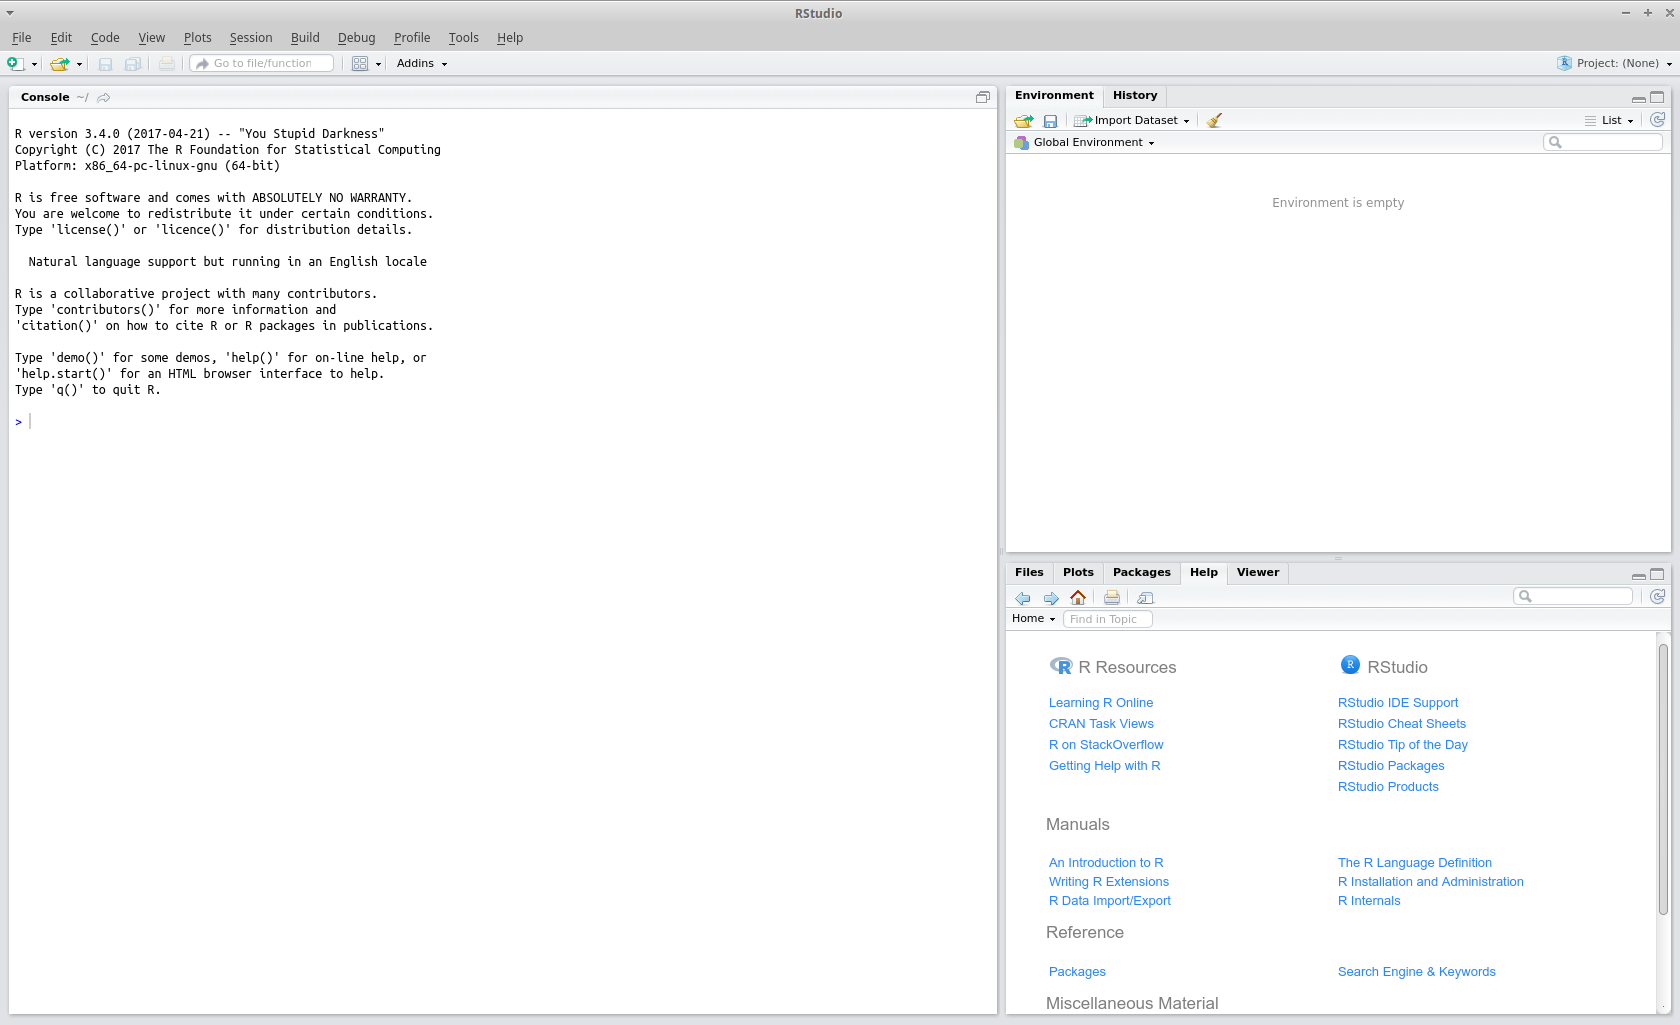
\includegraphics[width=0.8\linewidth]{Inhalte/images/RStudio-Screenshot-3-4} \end{center}

Links, in der \emph{Console} werden die Befehle eingegeben. Rechts oben
können Sie z. B. die Daten, aber auch andere Objekte, mit denen Sie
arbeiten, betrachten, auch die Historie der Befehle wird dort angezeigt.
Rechts unten können Sie u. a. Dateien und Abbildungen auswählen, aber
auch Hilfeseiten und Tipps betrachten.

Wir werden zunächst in der Konsole arbeiten.

Ein paar Anmerkungen vorweg:

\begin{itemize}
\tightlist
\item
  R unterscheidet zwischen Groß- und Kleinbuchstaben, d.~h.,
  \texttt{Oma} und \texttt{oma} sind zwei verschiedene Dinge für R!
\item
  R verwendet den Punkt \texttt{.} als Dezimaltrennzeichen,
\item
  Fehlende Werte werden in R durch \texttt{NA} kodiert,
\item
  Kommentare werden mit dem Rautezeichen \texttt{\#} eingeleitet; der
  Rest der Zeile von von R dann ignoriert.
\item
  R wendet Befehle direkt an.
\item
  R ist objektorientiert, d.~h., dieselbe Funktion hat evtl. je nach
  Funktionsargument unterschiedliche Rückgabewerte
\item
  Hilfe zu einem Befehl erhält man über ein vorgestelltes Fragezeichen
  \texttt{?}
\item
  Zusätzliche Funktionalität kann über Zusatzpakete hinzugeladen werden.
  Diese müssen ggf. zunächst installiert werden,
\item
  Mit der Pfeiltaste nach oben können Sie einen vorherigen Befehl wieder
  aufrufen,
\item
  Sofern Sie das Skriptfenster verwenden: einzelne Befehle aus dem
  Skriptfenster in R Studio können Sie auch mit \texttt{Str} und
  \texttt{Enter} an die Console schicken,
\end{itemize}

\hypertarget{r-als-taschenrechner}{%
\section{R als Taschenrechner}\label{r-als-taschenrechner}}

Auch wenn Statistik nicht Mathe ist, so kann man mit R auch rechnen.
Geben Sie zum Üben die Befehle in der R Konsole hinter der
Eingabeaufforderung \texttt{\textgreater{}} ein und beenden Sie die
Eingabe mit \texttt{Return} bzw. \texttt{Enter}.

\begin{Shaded}
\begin{Highlighting}[]
\DecValTok{4}\OperatorTok{+}\DecValTok{2}
\end{Highlighting}
\end{Shaded}

\begin{verbatim}
## [1] 6
\end{verbatim}

Das Ergebnis wird direkt angezeigt. Bei

\begin{Shaded}
\begin{Highlighting}[]
\NormalTok{x <-}\StringTok{ }\DecValTok{4}\OperatorTok{+}\DecValTok{2}
\end{Highlighting}
\end{Shaded}

erscheint zunächst kein Ergebnis. Über \texttt{\textless{}-} wird der
Variable \texttt{x} der Wert \texttt{4+2} zugewiesen. Wenn Sie jetzt

\begin{Shaded}
\begin{Highlighting}[]
\NormalTok{x}
\end{Highlighting}
\end{Shaded}

eingeben, wird das Ergebnis

\begin{verbatim}
## [1] 6
\end{verbatim}

angezeigt. Sie können jetzt auch mit \texttt{x} weiterrechnen.

\begin{Shaded}
\begin{Highlighting}[]
\NormalTok{x}\OperatorTok{/}\DecValTok{4}
\end{Highlighting}
\end{Shaded}

\begin{verbatim}
## [1] 1.5
\end{verbatim}

Vielleicht fragen Sie sich was die \texttt{{[}1{]}} vor dem Ergebnis
bedeutet. R arbeitet vektororientiert, und die \texttt{{[}1{]}} zeigt
an, dass es sich um das erste (und hier auch letzte) Element des Vektors
handelt.

\hypertarget{r-zur-datenanalyse}{%
\section{R zur Datenanalyse}\label{r-zur-datenanalyse}}

Wir wollen R aber als Tool zur Datenanalyse verwenden. Daher müssen wir
zunächst Daten einlesen.

Zunächst laden wir die Daten als \texttt{csv} Datei herunter

\begin{Shaded}
\begin{Highlighting}[]
\KeywordTok{download.file}\NormalTok{(}\StringTok{"https://goo.gl/whKjnl"}\NormalTok{, }\DataTypeTok{destfile =} \StringTok{"tips.csv"}\NormalTok{)}
\end{Highlighting}
\end{Shaded}

Der Inhalt der Datei ist jetzt als Tabelle \texttt{tips} in R verfügbar.

\href{https://github.com/luebby/Datenanalyse-mit-R/blob/master/Daten/tips-help.pdf}{Hier}
können Sie mehr über die Daten erfahren.

Das Einlesen von \texttt{csv} Dateien aus dem Arbeitsverzeichnis in R
kann erfolgen über

\begin{Shaded}
\begin{Highlighting}[]
\NormalTok{tips <-}\StringTok{ }\KeywordTok{read.csv2}\NormalTok{(}\StringTok{"tips.csv"}\NormalTok{)}
\end{Highlighting}
\end{Shaded}

Wo das lokale Verzeichnis (\enquote{working directory}) ist, können Sie
über

\begin{Shaded}
\begin{Highlighting}[]
\KeywordTok{getwd}\NormalTok{()}
\end{Highlighting}
\end{Shaded}

erfahren.

Der Datensatz \texttt{tips} taucht jetzt im \texttt{Enviroment} Fenster
rechts oben in RStudio auf. Durch Klicken auf den Namen können Sie diese
betrachten.

\begin{center}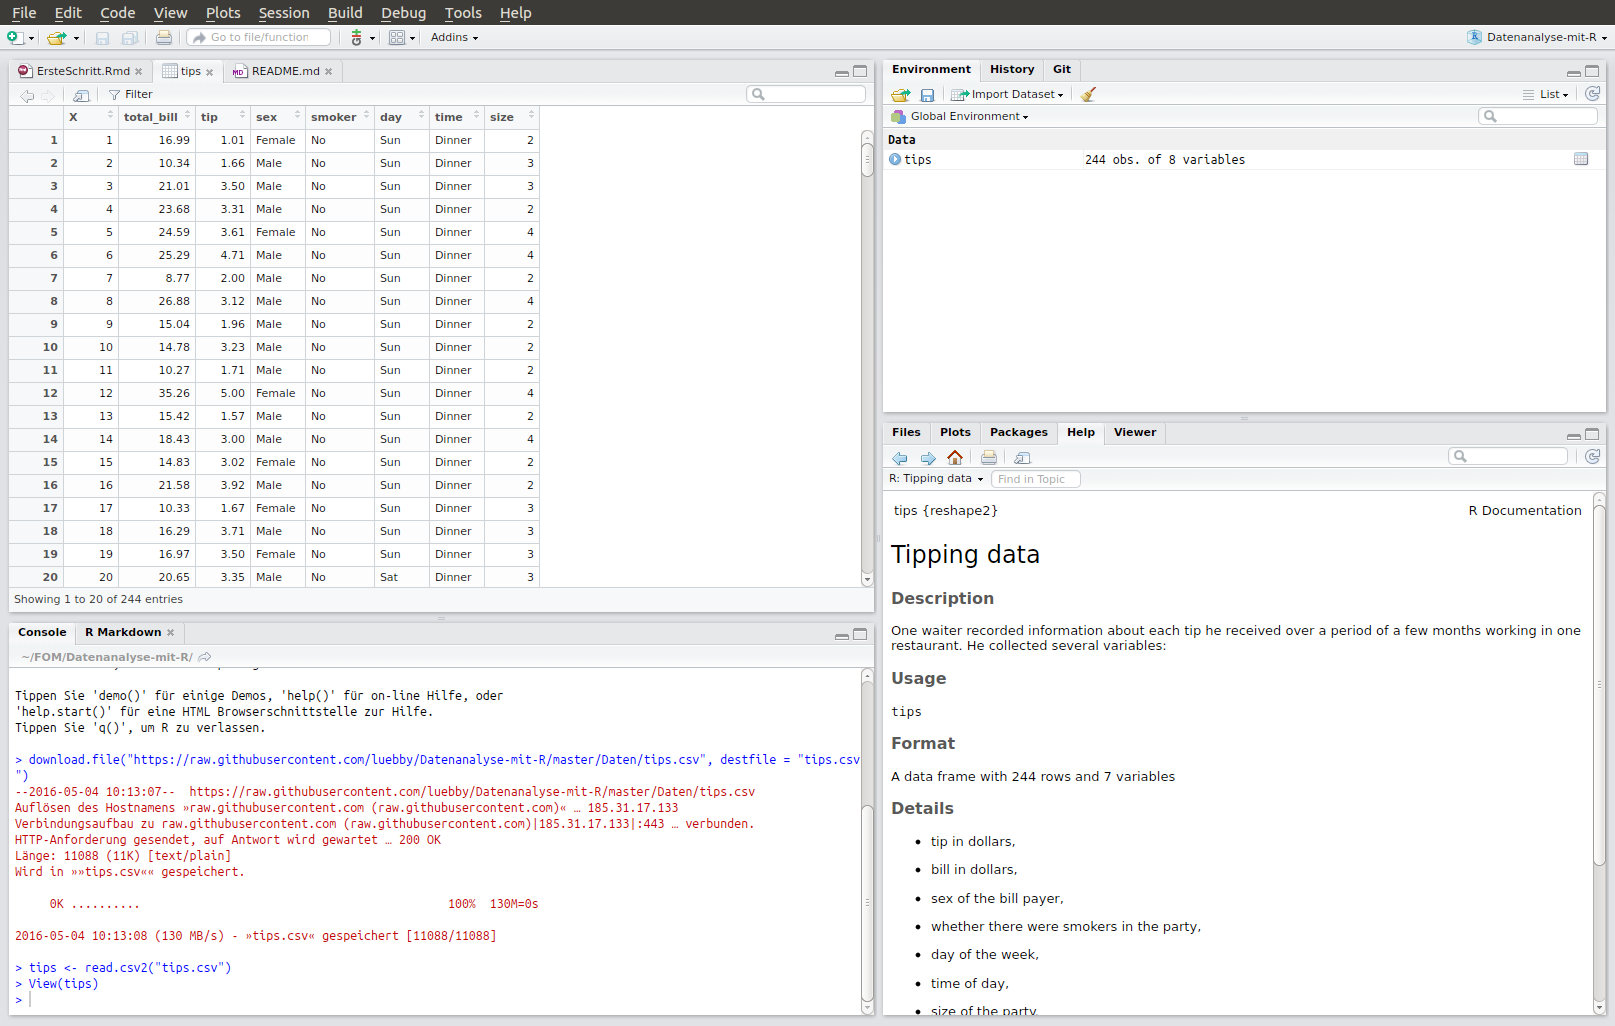
\includegraphics[width=0.8\linewidth]{Inhalte/images/tips-Enviroment} \end{center}

Alternativ können Sie Daten in RStudio komfortabel mit dem Button
\texttt{Import\ Dataset} (im Fenster \texttt{Environment} oder über das
Menü \texttt{File}) öffnen.

\hypertarget{erste-analyse-des-tips-datensatzes}{%
\section{Erste Analyse des tips
Datensatzes}\label{erste-analyse-des-tips-datensatzes}}

Dieser Datensatz aus

\emph{Bryant, P. G. and Smith, M (1995) Practical Data Analysis: Case
Studies in Business Statistics. Homewood, IL: Richard D. Irwin
Publishing}

enthält Trinkgelddaten. Diese sind in tabellarischer Form dargestellt,
d.~h. üblicherweise, dass die Beobachtungen zeilenweise untereinander
stehen, die einzelnen Variablen spaltenweise nebeneinander. In R heißen
solche Daten \emph{data frame}. Um einen ersten Überblick über die
verschiedenen Variablen zu erhalten geben wir den Befehl \texttt{str()}
ein:

\begin{Shaded}
\begin{Highlighting}[]
\KeywordTok{str}\NormalTok{(tips)}
\end{Highlighting}
\end{Shaded}

\begin{verbatim}
## 'data.frame':    244 obs. of  7 variables:
##  $ total_bill: num  17 10.3 21 23.7 24.6 ...
##  $ tip       : num  1.01 1.66 3.5 3.31 3.61 4.71 2 3.12 1.96 3.23 ...
##  $ sex       : Factor w/ 2 levels "Female","Male": 1 2 2 2 1 2 2 2 2 2 ...
##  $ smoker    : Factor w/ 2 levels "No","Yes": 1 1 1 1 1 1 1 1 1 1 ...
##  $ day       : Factor w/ 4 levels "Fri","Sat","Sun",..: 3 3 3 3 3 3 3 3 3 3 ...
##  $ time      : Factor w/ 2 levels "Dinner","Lunch": 1 1 1 1 1 1 1 1 1 1 ...
##  $ size      : int  2 3 3 2 4 4 2 4 2 2 ...
\end{verbatim}

Dieser enthält also 244 Zeilen (Beobachtungen) und 7 Spalten
(Variablen). Alternativ kann man diese Information auch über

\begin{Shaded}
\begin{Highlighting}[]
\KeywordTok{dim}\NormalTok{(tips)}
\end{Highlighting}
\end{Shaded}

\begin{verbatim}
## [1] 244   7
\end{verbatim}

erhalten.

Numerische (metrische) Variablen sind in R in der Regel vom Typ
\texttt{numeric} (stetig) oder \texttt{int} (Ganze Zahlen), kategorielle
(nominale, ordinale) Variablen vom Typ \texttt{factor} (bei ordinal:
Option \texttt{ordered\ =\ TRUE}) oder \texttt{character}.
\texttt{str()} und \texttt{dim()} sind erste Befehle, d.~h., Funktionen
in R, denen in der Klammer das jeweilige Funktionsargument übergeben
wird.

\begin{Shaded}
\begin{Highlighting}[]
\KeywordTok{head}\NormalTok{(tips) }\CommentTok{# Obere Zeilen}
\KeywordTok{tail}\NormalTok{(tips) }\CommentTok{# Untere Zeilen }
\end{Highlighting}
\end{Shaded}

ermöglichen ebenfalls einen Einblick über die Daten. Der Befehl

\begin{Shaded}
\begin{Highlighting}[]
\KeywordTok{names}\NormalTok{(tips)}
\end{Highlighting}
\end{Shaded}

gibt die Variablennamen zurück. Mit Hilfe des \texttt{\$} Operators kann
auf einzelne Variablen eines Dataframes zugegriffen werden. Mit

\begin{Shaded}
\begin{Highlighting}[]
\NormalTok{tips}\OperatorTok{$}\NormalTok{sex}
\end{Highlighting}
\end{Shaded}

erhalten Sie bspw. das Geschlecht des Rechnungszahlers.

\begin{center}\rule{0.5\linewidth}{\linethickness}\end{center}

\textbf{Übung:} Lassen Sie sich die Variable Rechnungshöhe
(\texttt{total\_bill}) anzeigen.

\begin{center}\rule{0.5\linewidth}{\linethickness}\end{center}

\hypertarget{mosaic}{%
\subsection{mosaic}\label{mosaic}}

\texttt{mosaic} ist ein Zusatzpaket, welches die Analyse mit R
erleichtert. Sofern noch nicht geschehen, muss es \emph{einmalig} über

\begin{Shaded}
\begin{Highlighting}[]
\KeywordTok{install.packages}\NormalTok{(}\StringTok{"mosaic"}\NormalTok{)}
\end{Highlighting}
\end{Shaded}

installiert werden.

Um es verwenden zu können, muss es -- wie jedes Paket -- für \emph{jede}
neue R-Sitzung über \texttt{library(mosaic)}geladen werden. Die
angegebenen Hinweise sind keine Fehlermeldung!

\begin{Shaded}
\begin{Highlighting}[]
\KeywordTok{library}\NormalTok{(mosaic)}
\end{Highlighting}
\end{Shaded}

Sollte beim Laden eines Paketes eine Meldung wie

\begin{Shaded}
\begin{Highlighting}[]
\KeywordTok{library}\NormalTok{(xyz)}
\end{Highlighting}
\end{Shaded}

\begin{verbatim}
## Error in library(xyz): there is no package called 'xyz'
\end{verbatim}

erscheinen, muss das Paket \texttt{xyz} zunächst installiert werden
(siehe oben).

Der Grundgedanke von \texttt{mosaic} ist \emph{Modellierung}. In R und
insbesondere in mosaic wird dafür die Tilde \texttt{\textasciitilde{}}
verwendet. \texttt{y\textasciitilde{}x} kann dabei gelesen werden wie
\enquote{y ist eine Funktion von x}. Um beispielsweise eine Abbildung
(Scatterplot) des Trinkgeldes \texttt{tip} (auf der Y-Achse) und
Rechnungshöhe \texttt{total\_bill} (auf der X-Achse) zu erhalten, kann
man in R folgenden Befehl eingeben:

\begin{Shaded}
\begin{Highlighting}[]
\KeywordTok{gf_point}\NormalTok{(tip }\OperatorTok{~}\StringTok{ }\NormalTok{total_bill, }\DataTypeTok{data=}\NormalTok{tips)}
\end{Highlighting}
\end{Shaded}

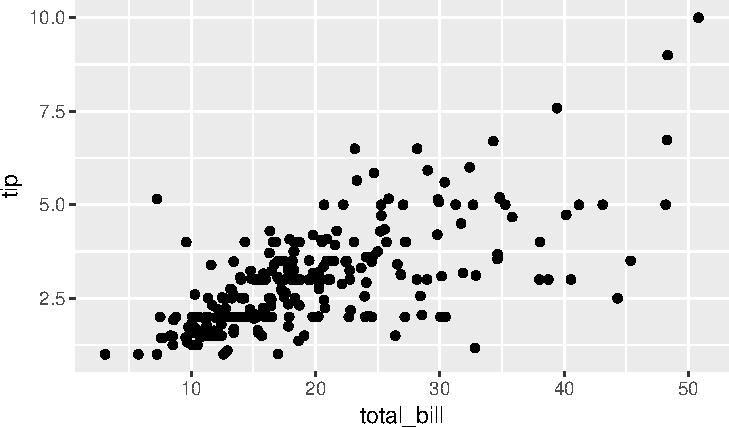
\includegraphics{DatenerhebungStatistik-Uebung_files/figure-latex/unnamed-chunk-28-1.pdf}

Das Argument \texttt{data=tips} stellt klar, aus welchen Datensatz die
Variablen kommen. Die Abbildung ist im RStudio jetzt rechts unten im
Reiter \emph{Plots} zu sehen.

\begin{center}\rule{0.5\linewidth}{\linethickness}\end{center}

\textbf{Übung:} Wie würden Sie den Trend beschreiben?

\begin{center}\rule{0.5\linewidth}{\linethickness}\end{center}

Wie oben erwähnt können wir R auch gut als Taschenrechner benutzen,
sollten aber bedenken, dass R vektorweise arbeitet. D. h.

\begin{Shaded}
\begin{Highlighting}[]
\NormalTok{tips}\OperatorTok{$}\NormalTok{tip}\OperatorTok{/}\NormalTok{tips}\OperatorTok{$}\NormalTok{total_bill}
\end{Highlighting}
\end{Shaded}

gibt für \emph{jede Beobachtung} die relative Trinkgeldhöhe bezogen auf
die Rechnungshöhe an. Über

\begin{Shaded}
\begin{Highlighting}[]
\NormalTok{(tips}\OperatorTok{$}\NormalTok{tip}\OperatorTok{/}\NormalTok{tips}\OperatorTok{$}\NormalTok{total_bill)}\OperatorTok{<}\FloatTok{0.10}
\end{Highlighting}
\end{Shaded}

erhalten wir einen Vektor vom Typ \texttt{logical}. Dieser nimmt nur
zwei Werte an, nämlich \texttt{TRUE} und \texttt{FALSE}, je nach dem, ob
der jeweilige Wert kleiner als 0.10 ist oder nicht. Neben
\texttt{\textless{}} und \texttt{\textgreater{}} bzw.
\texttt{\textless{}=} und \texttt{\textgreater{}=} gibt es ja auch noch
die Prüfung auf Gleichheit. Hierfür werden in R gleich \emph{zwei}
Gleichheitszeichen verwendet, also \texttt{==}.

\begin{center}\rule{0.5\linewidth}{\linethickness}\end{center}

\textbf{Übung:} Was gibt folgender der Befehl zurück?

\begin{Shaded}
\begin{Highlighting}[]
\NormalTok{tips}\OperatorTok{$}\NormalTok{sex}\OperatorTok{==}\StringTok{"Female"} 
\end{Highlighting}
\end{Shaded}

\begin{center}\rule{0.5\linewidth}{\linethickness}\end{center}

Logische Vektoren können z. B. mit \enquote{und} \texttt{\&} oder
\enquote{oder} \texttt{\textbar{}} verknüpft werden:

\begin{Shaded}
\begin{Highlighting}[]
\NormalTok{tips}\OperatorTok{$}\NormalTok{sex}\OperatorTok{==}\StringTok{"Female"} \OperatorTok{&}\StringTok{ }\NormalTok{tips}\OperatorTok{$}\NormalTok{smoker}\OperatorTok{==}\StringTok{"Yes"}
\end{Highlighting}
\end{Shaded}

gibt die Tischgesellschaften als \texttt{TRUE} wieder, in denen die
Rechnung von Frauen beglichen wurde \emph{und} geraucht wurde,

\begin{Shaded}
\begin{Highlighting}[]
\NormalTok{tips}\OperatorTok{$}\NormalTok{sex}\OperatorTok{==}\StringTok{"Female"} \OperatorTok{|}\StringTok{ }\NormalTok{tips}\OperatorTok{$}\NormalTok{smoker}\OperatorTok{==}\StringTok{"Yes"}
\end{Highlighting}
\end{Shaded}

gibt die Tischgesellschaften als \texttt{TRUE} wieder, in denen die
Rechnung von Frauen beglichen wurde \emph{oder} geraucht wurde.

Intern wird \texttt{TRUE} in R mit der Zahl 1 hinterlegt, \texttt{FALSE}
mit 0. Mit dem Befehl \texttt{sum()} kann man daher die Elemente eines
Vektor aufsummieren, also erfahren wir über

\begin{Shaded}
\begin{Highlighting}[]
\KeywordTok{sum}\NormalTok{(tips}\OperatorTok{$}\NormalTok{sex}\OperatorTok{==}\StringTok{"Female"} \OperatorTok{&}\StringTok{ }\NormalTok{tips}\OperatorTok{$}\NormalTok{smoker}\OperatorTok{==}\StringTok{"Yes"}\NormalTok{)}
\end{Highlighting}
\end{Shaded}

dass bei 33 Tischgesellschaften bei denen geraucht wurde, eine Frau die
Rechnung bezahlte. Im Verhältnis zu allen Tischgesellschaften, bei denen
eine Frau zahlte, liegt der Raucheranteil also bei 0.3793103:

\begin{Shaded}
\begin{Highlighting}[]
\KeywordTok{sum}\NormalTok{(tips}\OperatorTok{$}\NormalTok{sex}\OperatorTok{==}\StringTok{"Female"} \OperatorTok{&}\StringTok{ }\NormalTok{tips}\OperatorTok{$}\NormalTok{smoker}\OperatorTok{==}\StringTok{"Yes"}\NormalTok{) }\OperatorTok{/}\StringTok{ }\KeywordTok{sum}\NormalTok{(tips}\OperatorTok{$}\NormalTok{sex}\OperatorTok{==}\StringTok{"Female"}\NormalTok{)}
\end{Highlighting}
\end{Shaded}

\begin{center}\rule{0.5\linewidth}{\linethickness}\end{center}

\textbf{Übung:} Wurde bei den Tischgesellschaften, bei denen ein Mann
zahlte, relativ häufiger geraucht als bei den Frauen?

\begin{center}\rule{0.5\linewidth}{\linethickness}\end{center}

\hypertarget{ubung-teaching-rating}{%
\section{Übung: Teaching Rating}\label{ubung-teaching-rating}}

Dieser Datensatz analysiert u. a. den Zusammenhang zwischen Schönheit
und Evaluierungsergebnis:

\emph{Hamermesh, D.S., and Parker, A. (2005). Beauty in the Classroom:
Instructors' Pulchritude and Putative Pedagogical Productivity.
Economics of Education Review, 24, 369--376.}

Sie können ihn von \url{https://goo.gl/6Y3KoK} herunterladen.
\href{https://github.com/luebby/Datenanalyse-mit-R/blob/master/Daten/TeachingRatings-help.pdf}{Hier}
gibt es eine Beschreibung. Anders als im Paper (und im Paket
\texttt{AER}) wird hier nur ein zufälliger Kurs je Dozent verwendet.

\begin{enumerate}
\def\labelenumi{\arabic{enumi}.}
\tightlist
\item
  Lesen Sie den Datensatz in R ein.
\item
  Wie viele Zeilen, wie viele Spalten liegen vor?
\item
  Wie heißen die Variablen?
\item
  Betrachten Sie visuell den Zusammenhang von dem Evaluierungsergebnis
  \texttt{eval} und Schönheit \texttt{beauty}. Was können Sie erkennen?
\item
  Sind relativ mehr Frauen oder mehr Männer (\texttt{gender}) in einem
  unbefristeten Arbeitsverhältnis (\emph{Tenure Track},
  \texttt{tenure})?
\end{enumerate}

\hypertarget{daten-importieren}{%
\section{Daten importieren}\label{daten-importieren}}

Der Datenimport in R ist in vielen unterschiedlichen Dateiformaten
möglich. Das \texttt{csv} Format eignet sich besonders zum Übertragen
von Datendateien. Im deutschsprachigen Raum wird dabei als
\emph{Dezimaltrennzeichen} das Komma \texttt{,} und als
\emph{Datentrennzeichen} das Semikolon \texttt{;} verwendet. In der
ersten Zeile sollten die Variablennamen stehen. Das Einlesen in einen R
Data-Frame (hier \texttt{meineDaten}) kann dann über

\begin{Shaded}
\begin{Highlighting}[]
\NormalTok{meineDaten <-}\StringTok{ }\KeywordTok{read.csv2}\NormalTok{(}\KeywordTok{file.choose}\NormalTok{()) }\CommentTok{# Datei auswählen}
\end{Highlighting}
\end{Shaded}

erfolgen.

Der Befehl \texttt{file.choose()} öffnet dabei den Dateiordner. Bei
\enquote{internationalen} \texttt{csv} Dateien ist das Datentrennzeichen
i. d.~R. ein Komma \texttt{,}, das Dezimaltrennzeichen ein Punkt
\texttt{.}. Hier funktioniert der Import in R dann über den Befehl
\texttt{read.csv}.

In R Studio gibt es im Reiter \texttt{Environment} im Fenster Rechts
oben einen Menüpunkt \texttt{Import\ Dataset} der mehr
Einstellmöglichkeiten bietet.

Excel Dateien können unter anderem mit Hilfe des Zusatzpaketes
\texttt{readxl} können eingelesen werden:

\begin{Shaded}
\begin{Highlighting}[]
\KeywordTok{library}\NormalTok{(readxl) }\CommentTok{# Paket laden}
\NormalTok{meineDaten <-}\StringTok{ }\KeywordTok{read_excel}\NormalTok{(}\KeywordTok{file.choose}\NormalTok{())  }\CommentTok{# Datei auswählen und in R einlesen}
\end{Highlighting}
\end{Shaded}

\href{https://www.fom.de/forschung/institute/ifes/studium-und-lehre.html\#!acc=datenquellen}{Hier}
finden Sie eine Linksammlung zu verschiedenen Datenquellen.

\hypertarget{literatur}{%
\section{Literatur}\label{literatur}}

\begin{itemize}
\tightlist
\item
  Nicholas J. Horton, Randall Pruim, Daniel T. Kaplan (2015): Project
  MOSAIC Little Books \emph{A Student's Guide to R}
  \url{https://github.com/ProjectMOSAIC/LittleBooks/raw/master/StudentGuide/MOSAIC-StudentGuide.pdf},
  Kapitel 1, 2, 13
\item
  Chester Ismay (2016): Getting used to R, RStudio, and R Markdown
  \url{https://ismayc.github.io/rbasics-book/}
\item
  Maike Luhmann (2015): \emph{R für Einsteiger}, Kapitel 1-8
\item
  Daniel Wollschläger (2014): \emph{Grundlagen der Datenanalyse mit R},
  Kapitel 1-4
\end{itemize}

\hypertarget{lizenz}{%
\subsection{Lizenz}\label{lizenz}}

Diese Übung wurde von Karsten Lübke entwickelt und orientiert sich an
der Übung zum Buch
\href{https://www.openintro.org/stat/index.php?stat_book=isrs}{OpenIntro}
von Andrew Bray, Mine Çetinkaya-Rundel und Mark Hansen und steht wie
diese unter der Lizenz
\href{http://creativecommons.org/licenses/by-sa/3.0}{Creative Commons
Attribution-ShareAlike 3.0 Unported}. Kleinere Ergänzungen stammen von
Norman Markgraf

\hypertarget{versionshinweise}{%
\subsection{Versionshinweise:}\label{versionshinweise}}

\begin{itemize}
\tightlist
\item
  Datum erstellt: 2019-01-24
\item
  R Version: 3.5.1
\item
  \texttt{mosaic} Version: 1.4.0
\end{itemize}

\hypertarget{kapitel-1-einfuhrung-in-daten}{%
\chapter{Kapitel 1: Einführung in
Daten}\label{kapitel-1-einfuhrung-in-daten}}

\hypertarget{datensatz}{%
\section{Datensatz}\label{datensatz}}

Wir werden jetzt den \emph{tips} Datensatz aus \emph{Bryant, P. G. and
Smith, M (1995) Practical Data Analysis: Case Studies in Business
Statistics. Homewood, IL: Richard D. Irwin Publishing} näher
analysieren.

Sofern noch nicht geschehen, können Sie ihn z. B.
\href{https://goo.gl/whKjnl}{hier} als \texttt{csv}-Datei direkt nach R
herunterladen:

\begin{Shaded}
\begin{Highlighting}[]
\KeywordTok{download.file}\NormalTok{(}\StringTok{"https://goo.gl/whKjnl"}\NormalTok{, }\DataTypeTok{destfile =} \StringTok{"tips.csv"}\NormalTok{)}
\end{Highlighting}
\end{Shaded}

Wenn sich die Daten auf Ihrem Computer gespeichert sind, können Sie sie
laden:

\begin{Shaded}
\begin{Highlighting}[]
\NormalTok{tips <-}\StringTok{ }\KeywordTok{read.csv2}\NormalTok{(}\StringTok{"tips.csv"}\NormalTok{)}
\end{Highlighting}
\end{Shaded}

Achtung: \texttt{read.csv} geht vom amerikanischen Format aus. Wenn es
sich um eine \enquote{deutsche CSV-Datei} handelt, verwenden Sie
\texttt{read.csv2}.

\emph{Tipp:} Wenn Sie nicht mehr wissen, wo die Daten liegen: statt
\texttt{tips.csv} den Befehl \texttt{file.choose()} als Argument für die
Funktion \texttt{read.csv2} verwenden.

Inwieweit das Einlesen wie gewünscht geklappt hat, kann über

\begin{Shaded}
\begin{Highlighting}[]
\KeywordTok{str}\NormalTok{(tips)}
\end{Highlighting}
\end{Shaded}

überprüft werden: Der Datensatz hat also 244 Zeilen (= Beobachtungen)
und 7 Spalten (= Merkmale/Variablen).

Zur folgenden Analyse muss zunächst das Paket \texttt{mosaic} geladen
werden:

\begin{Shaded}
\begin{Highlighting}[]
\KeywordTok{library}\NormalTok{(mosaic)}
\end{Highlighting}
\end{Shaded}

\hypertarget{grafische-verfahren-der-datenanalyse}{%
\section{Grafische Verfahren der
Datenanalyse}\label{grafische-verfahren-der-datenanalyse}}

Bevor evtl. wichtige Information in zusammenfassenden Kennzahlen
verloren geht, versuchen wir einen Gesamtüberblick zu erhalten.

\hypertarget{balkendiagramm}{%
\subsection{Balkendiagramm}\label{balkendiagramm}}

Balkendiagramme eignen sich am besten um Häufigkeiten darzustellen, also
für kategorielle Variablen (\texttt{factor}) oder für metrische
Variablen (\texttt{numeric}) mit wenigen Merkmalsausprägungen.

Um einen Überblick über die Geschlechterverteilung \texttt{sex} zu
bekommen kann die Funktion \texttt{gf\_bar} aus dem Paket
\texttt{mosaic} verwendet werden:

\begin{Shaded}
\begin{Highlighting}[]
\KeywordTok{gf_bar}\NormalTok{(}\OperatorTok{~}\StringTok{ }\NormalTok{sex, }\DataTypeTok{data=}\NormalTok{tips)}
\end{Highlighting}
\end{Shaded}

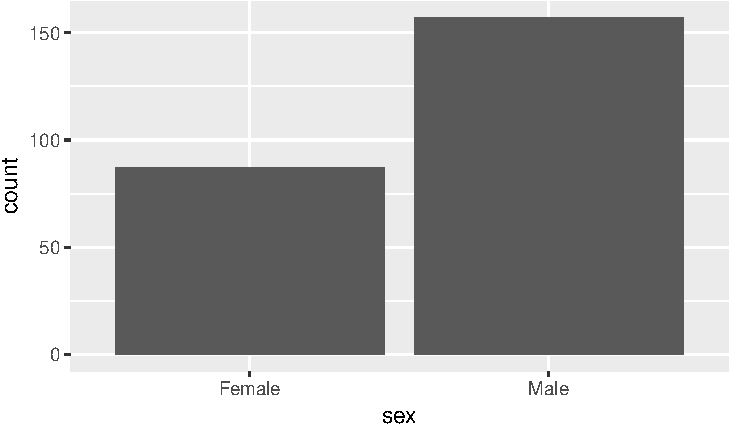
\includegraphics{DatenerhebungStatistik-Uebung_files/figure-latex/unnamed-chunk-42-1.pdf}

In mosaic wird (fast) immer die Formeldarstellung
\texttt{y\ \textasciitilde{}\ x\ \textbar{}\ z} verwendet: \texttt{y} in
Abhängigkeit von \texttt{x} (\texttt{y} wird modelliert durch
\texttt{x}), gruppiert nach den Werten von \texttt{z}, wobei einzelne
Teile fehlen können, so wie im Beispiel \texttt{y} und \texttt{z}. Aber
um z. B. die Verteilung des Geschlechts des Zahlenden je Tageszeit
\texttt{time} darzustellen muss hier eingegeben werden:

\begin{Shaded}
\begin{Highlighting}[]
\KeywordTok{gf_bar}\NormalTok{(}\OperatorTok{~}\StringTok{ }\NormalTok{sex }\OperatorTok{|}\StringTok{ }\NormalTok{time, }\DataTypeTok{data=}\NormalTok{tips)}
\end{Highlighting}
\end{Shaded}

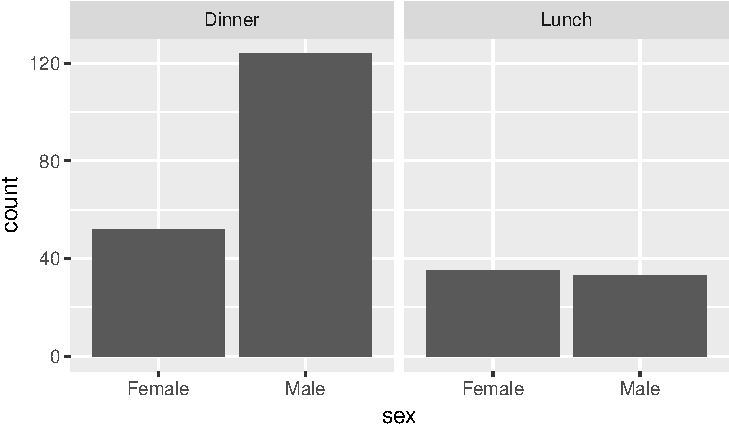
\includegraphics{DatenerhebungStatistik-Uebung_files/figure-latex/unnamed-chunk-43-1.pdf}

\begin{center}\rule{0.5\linewidth}{\linethickness}\end{center}

\textbf{Übung:}

\begin{enumerate}
\def\labelenumi{\arabic{enumi}.}
\tightlist
\item
  Zeichnen Sie ein Balkendiagramm des Rauchverhaltens \texttt{smoker} je
  Wochentag \texttt{day} und interpretieren Sie das Ergebnis.
\end{enumerate}

\begin{center}\rule{0.5\linewidth}{\linethickness}\end{center}

\hypertarget{histogramm}{%
\subsection{Histogramm}\label{histogramm}}

Histogramme werden für metrische Daten verwendet, der Befehl lautet
\texttt{histogram}.

\begin{center}\rule{0.5\linewidth}{\linethickness}\end{center}

\textbf{Übung:}

\begin{enumerate}
\def\labelenumi{\arabic{enumi}.}
\setcounter{enumi}{1}
\tightlist
\item
  Welche Abbildung wird über
\end{enumerate}

\begin{Shaded}
\begin{Highlighting}[]
\KeywordTok{gf_histogram}\NormalTok{(}\OperatorTok{~}\StringTok{ }\NormalTok{total_bill }\OperatorTok{|}\StringTok{ }\NormalTok{sex, }\DataTypeTok{data=}\NormalTok{tips)}
\end{Highlighting}
\end{Shaded}

erzeugt?

\begin{center}\rule{0.5\linewidth}{\linethickness}\end{center}

\textbf{Punktdiagramme} sind eine Variante von Histogrammen, die
besonders für metrische Variablen mit wenigen Merkmalsausprägungen
geeignet sind.

\begin{Shaded}
\begin{Highlighting}[]
\KeywordTok{gf_dotplot}\NormalTok{(}\OperatorTok{~}\StringTok{ }\NormalTok{size, }\DataTypeTok{binwidth=}\DecValTok{1}\OperatorTok{/}\DecValTok{55}\NormalTok{, }\DataTypeTok{data=}\NormalTok{tips)}
\end{Highlighting}
\end{Shaded}

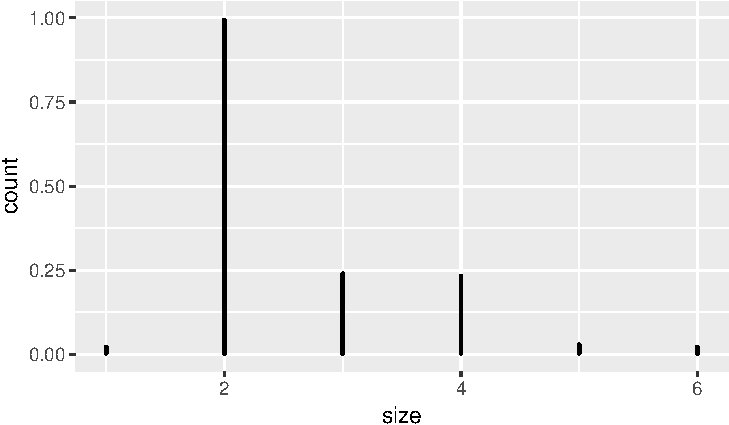
\includegraphics{DatenerhebungStatistik-Uebung_files/figure-latex/unnamed-chunk-45-1.pdf}

Hier wurde ein zusätzliche Parameter der Funktion \texttt{gf\_dotplot}
übergeben: \texttt{binwidth=1/55}. Dieser Parameter wurde wurde
verwendet, um die Abbildung schöner zu machen. Welche Optionen es gibt
und was diese bedeuten, kann man in R häufig einfach über die Hilfe,
hier also \texttt{?gf\_dotplot}, erfahren.

\hypertarget{boxplots}{%
\subsection{Boxplots}\label{boxplots}}

Boxplots zeigen nicht nur den Median (50\%-Quantil) sowie das obere
(75\%) und untere (25\%) Quartil - und damit den Interquartilsabstand -,
sondern geben auch Hinweise auf potentielle Ausreißer:

\begin{Shaded}
\begin{Highlighting}[]
\KeywordTok{gf_boxplot}\NormalTok{(total_bill }\OperatorTok{~}\StringTok{ }\NormalTok{sex, }\DataTypeTok{data=}\NormalTok{tips)}
\end{Highlighting}
\end{Shaded}

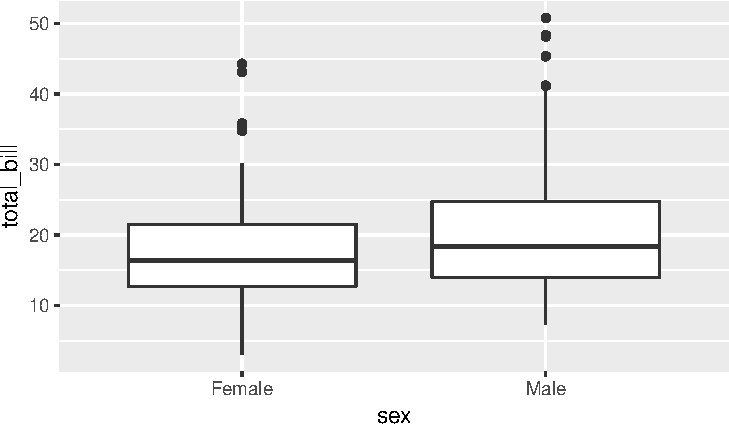
\includegraphics{DatenerhebungStatistik-Uebung_files/figure-latex/unnamed-chunk-46-1.pdf}

und gruppiert nach Tageszeit:

\begin{Shaded}
\begin{Highlighting}[]
\KeywordTok{gf_boxplot}\NormalTok{(total_bill }\OperatorTok{~}\StringTok{ }\NormalTok{sex }\OperatorTok{|}\StringTok{ }\NormalTok{time, }\DataTypeTok{data=}\NormalTok{tips)}
\end{Highlighting}
\end{Shaded}

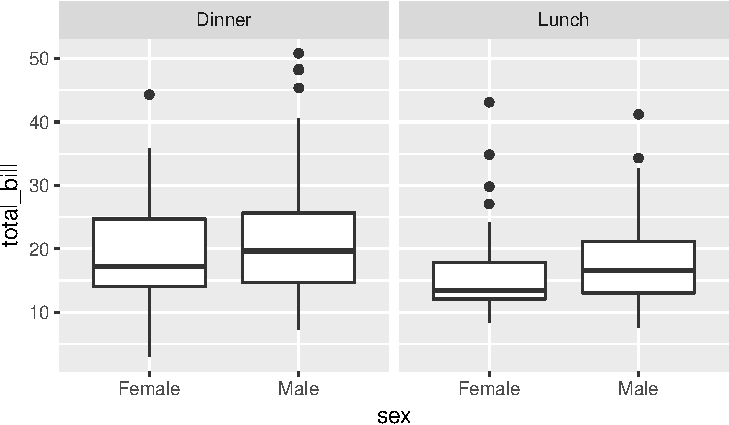
\includegraphics{DatenerhebungStatistik-Uebung_files/figure-latex/unnamed-chunk-47-1.pdf}

\begin{center}\rule{0.5\linewidth}{\linethickness}\end{center}

\textbf{Übung:}

\begin{enumerate}
\def\labelenumi{\arabic{enumi}.}
\setcounter{enumi}{2}
\tightlist
\item
  Zeichen Sie einen Boxplot für die Trinkgeldhöhe \texttt{tip} in
  Abhängigkeit davon, ob geraucht wurde (\texttt{smoker}). Gibt es
  Unterschiede in der Trinkgeldhöhe und, wenn ja, in welchem Bereich?
\end{enumerate}

\begin{center}\rule{0.5\linewidth}{\linethickness}\end{center}

\hypertarget{scatterplot-streudiagramme}{%
\subsection{Scatterplot
(Streudiagramme)}\label{scatterplot-streudiagramme}}

Streudiagramme sind besonders gut geeignet, um einen Überblick auf den
Zusammenhang zweier metrischer Merkmale zu erhalten; beispielsweise um
den Zusammenhang von \texttt{tip} und \texttt{total\_bill} zu
analysieren.

\begin{Shaded}
\begin{Highlighting}[]
\KeywordTok{gf_point}\NormalTok{(tip }\OperatorTok{~}\StringTok{ }\NormalTok{total_bill, }\DataTypeTok{data=}\NormalTok{tips)}
\end{Highlighting}
\end{Shaded}

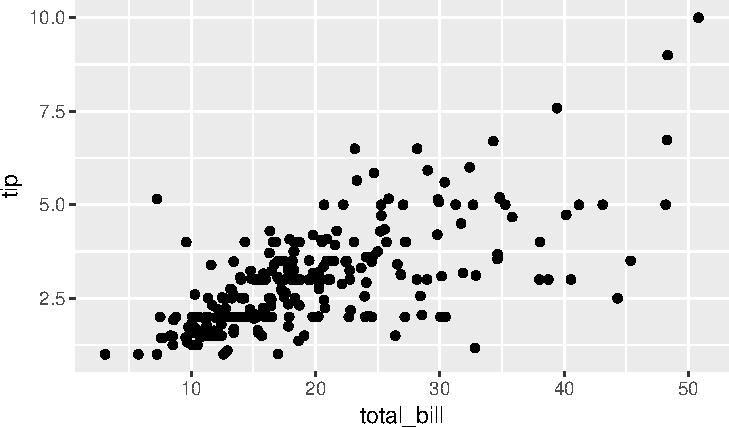
\includegraphics{DatenerhebungStatistik-Uebung_files/figure-latex/unnamed-chunk-48-1.pdf}

Wenig überraschend steigt die Trinkgeldhöhe mit der Rechnung. Wie sieht
es relativ aus? Dazu müssen wir zunächst ein neues Merkmal im Datensatz
erzeugen, z. B.:

\begin{Shaded}
\begin{Highlighting}[]
\NormalTok{tips}\OperatorTok{$}\NormalTok{tip_relativ <-}\StringTok{ }\NormalTok{tips}\OperatorTok{$}\NormalTok{tip }\OperatorTok{/}\StringTok{ }\NormalTok{tips}\OperatorTok{$}\NormalTok{total_bill}
\end{Highlighting}
\end{Shaded}

Im Datensatz \texttt{tips} wird der (neuen) Variable
\texttt{tip\_relativ} der Quotient aus Trinkgeld und Rechnungshöhe
zugewiesen.

\begin{center}\rule{0.5\linewidth}{\linethickness}\end{center}

\textbf{Übung:}

\begin{enumerate}
\def\labelenumi{\arabic{enumi}.}
\setcounter{enumi}{3}
\tightlist
\item
  Erstellen Sie eine Abbildung, mit der Sie visuell gucken können, wie
  der Zusammenhang zwischen der relativen Trinkgeldhöhe (abhängige
  Variable) und der Rechnungshöhe (uanbhängige Variable) aussieht, und
  ob sich dieser je nach Geschlecht des Rechnungszahlers unterscheidet.
\end{enumerate}

\begin{center}\rule{0.5\linewidth}{\linethickness}\end{center}

\hypertarget{mosaicplot}{%
\subsection{Mosaicplot}\label{mosaicplot}}

Mosaicplots eignen sich, um den Zusammenhang zwischen kategoriellen
Variablen darzustellen. Zunächst müssen wir dazu eine Kreuztabelle
erstellen. Das geht in \texttt{mosaic} über den Befehl \texttt{tally}.
Dieser Befehl ist recht mächtig -- dazu später mehr. Wir erzeugen eine
solche Kreuztabelle zwischen Tageszeit und Rauchen über

\begin{Shaded}
\begin{Highlighting}[]
\NormalTok{tab_smoke_time <-}\StringTok{ }\KeywordTok{tally}\NormalTok{(smoker }\OperatorTok{~}\StringTok{ }\NormalTok{time, }\DataTypeTok{data=}\NormalTok{tips)}
\end{Highlighting}
\end{Shaded}

Dem (neuen) R Objekt \texttt{tab\_smoke\_time} wird also das Ergebnis
des \texttt{tally} Befehls zugewiesen. Wie das Ergebnis aussieht, und
welchen Typ es hat erfahren wir über

\begin{Shaded}
\begin{Highlighting}[]
\KeywordTok{print}\NormalTok{(tab_smoke_time)}
\end{Highlighting}
\end{Shaded}

\begin{verbatim}
##       time
## smoker Dinner Lunch
##    No     106    45
##    Yes     70    23
\end{verbatim}

\begin{Shaded}
\begin{Highlighting}[]
\KeywordTok{str}\NormalTok{(tab_smoke_time)}
\end{Highlighting}
\end{Shaded}

\begin{verbatim}
##  'table' int [1:2, 1:2] 106 70 45 23
##  - attr(*, "dimnames")=List of 2
##   ..$ smoker: chr [1:2] "No" "Yes"
##   ..$ time  : chr [1:2] "Dinner" "Lunch"
\end{verbatim}

Es handelt sich also um eine Tabelle (\texttt{table}) der Dimension 2,
2, also 2 Zeilen, 2 Spalten.

Der Befehl für einen Mosaicplot lautet \texttt{mosaicplot}:

\begin{Shaded}
\begin{Highlighting}[]
\KeywordTok{mosaicplot}\NormalTok{(tab_smoke_time)}
\end{Highlighting}
\end{Shaded}

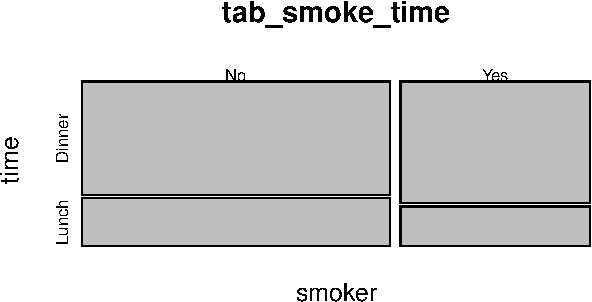
\includegraphics{DatenerhebungStatistik-Uebung_files/figure-latex/unnamed-chunk-52-1.pdf}

\hypertarget{korrelationsplot}{%
\subsection{Korrelationsplot}\label{korrelationsplot}}

Mit Hilfe des Zusatzpakets \texttt{corrplot} lassen sich Korrelationen
besonders einfach visualisieren. Das Paket muss wie jedes Paket
\emph{einmalig} über

\begin{Shaded}
\begin{Highlighting}[]
\KeywordTok{install.packages}\NormalTok{(}\StringTok{"corrplot"}\NormalTok{)}
\end{Highlighting}
\end{Shaded}

installiert werden -- wiederum werden evt. weitere benötigte Pakete
mit-installiert. Nach dem Laden des Pakets über

\begin{Shaded}
\begin{Highlighting}[]
\KeywordTok{library}\NormalTok{(corrplot)}
\end{Highlighting}
\end{Shaded}

kann dies über

\begin{Shaded}
\begin{Highlighting}[]
\KeywordTok{corrplot}\NormalTok{(}\KeywordTok{cor}\NormalTok{(tips[,}\KeywordTok{c}\NormalTok{(}\StringTok{"total_bill"}\NormalTok{, }\StringTok{"tip"}\NormalTok{, }\StringTok{"size"}\NormalTok{)]))}
\end{Highlighting}
\end{Shaded}

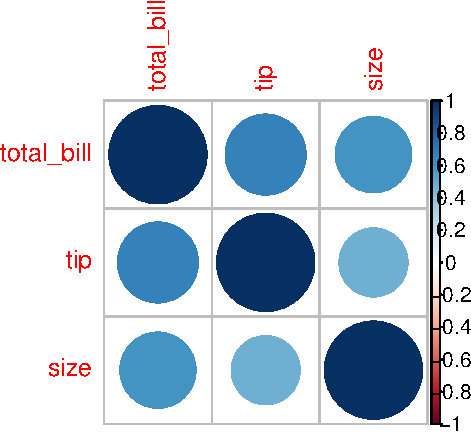
\includegraphics{DatenerhebungStatistik-Uebung_files/figure-latex/unnamed-chunk-55-1.pdf}

gezeichnet werden. Je intensiver die Farbe, desto höher die Korrelation.
Hier gibt es unzählige Einstellmöglichkeiten, siehe \texttt{?corrplot}
bzw. für Beispiele:

\begin{Shaded}
\begin{Highlighting}[]
\KeywordTok{vignette}\NormalTok{(}\StringTok{"corrplot-intro"}\NormalTok{)}
\end{Highlighting}
\end{Shaded}

\hypertarget{kennzahlen-der-datenanalyse}{%
\section{Kennzahlen der
Datenanalyse}\label{kennzahlen-der-datenanalyse}}

Nachdem wir einen ersten visuellen Eindruck gewonnen haben, wollen wir
uns jetzt Kennzahlen widmen.

\hypertarget{lagemae}{%
\subsection{Lagemaße}\label{lagemae}}

Das Minimum und Maximum von metrischen Daten kann einfach durch
\texttt{min} bzw. \texttt{max} bestimmt werden, in \texttt{mosaic} auch
\enquote{modelliert}:

\begin{Shaded}
\begin{Highlighting}[]
\KeywordTok{min}\NormalTok{(}\OperatorTok{~}\StringTok{ }\NormalTok{total_bill }\OperatorTok{|}\StringTok{ }\NormalTok{smoker, }\DataTypeTok{data=}\NormalTok{tips)}
\end{Highlighting}
\end{Shaded}

\begin{verbatim}
##   No  Yes 
## 7.25 3.07
\end{verbatim}

gibt also das Minimum der Rechnungshöhe, getrennt nach Raucher und
Nichtrauchern an, d.~h. das Minimum bei den Rauchern lag bei 3.07\$.

\begin{center}\rule{0.5\linewidth}{\linethickness}\end{center}

\textbf{Übung:}

\begin{enumerate}
\def\labelenumi{\arabic{enumi}.}
\setcounter{enumi}{4}
\tightlist
\item
  Bestimmen Sie das Maximum der Trinkgeldhöhe je Wochentag
  (\texttt{day})
\end{enumerate}

\begin{center}\rule{0.5\linewidth}{\linethickness}\end{center}

Lagemaße sollen die zentrale Tendenz der Daten beschreiben. Gebräuchlich
sind in der Regel der arithmetische Mittelwert \texttt{mean}
\[\bar{x}=\frac{1}{n}\sum_{i=1}^{n}x_i=\frac{x_1+x_2+x_3+\cdots+x_n}{n}\]

\begin{Shaded}
\begin{Highlighting}[]
\KeywordTok{mean}\NormalTok{(}\OperatorTok{~}\StringTok{ }\NormalTok{total_bill, }\DataTypeTok{data=}\NormalTok{tips)}
\end{Highlighting}
\end{Shaded}

\begin{verbatim}
## [1] 19.78594
\end{verbatim}

sowie der Median (Zentralwert) \texttt{median}:

\begin{Shaded}
\begin{Highlighting}[]
\KeywordTok{median}\NormalTok{(}\OperatorTok{~}\StringTok{ }\NormalTok{total_bill, }\DataTypeTok{data=}\NormalTok{tips)}
\end{Highlighting}
\end{Shaded}

\begin{verbatim}
## [1] 17.795
\end{verbatim}

Den jeweiligen Rang der Beonbachtungen erhalten Sie über

\begin{Shaded}
\begin{Highlighting}[]
\KeywordTok{rank}\NormalTok{(tips}\OperatorTok{$}\NormalTok{total_bill)}
\end{Highlighting}
\end{Shaded}

\begin{verbatim}
##   [1] 113.0  25.5 162.5 179.0 187.0 192.0  12.0 199.0  82.0  79.0  21.0
##  [12] 229.0  86.0 136.0  80.0 166.0  23.5 100.0 112.0 156.0 126.5 151.5
##  [23]  91.0 234.0 147.0 123.0  62.0  51.0 167.0 144.0  13.0 135.0  83.0
##  [34] 157.5 122.0 182.0 101.0 111.0 138.0 217.0  97.0 118.0  70.0  15.0
##  [45] 215.0 133.5 169.0 220.0 207.0 128.0  48.0  22.0 227.0  17.0 193.0
##  [56] 143.0 231.0 196.0  34.0 242.0 151.5  68.5  32.0 133.5 121.0 148.0
##  [67] 105.0   1.0 149.0  81.0  41.0 114.0 198.0 191.0  78.0  27.0 126.5
##  [78] 202.0 174.0 116.0 142.0 109.0  18.5 221.0  94.5 228.0  57.0 132.0
##  [89] 188.0 164.0 208.0 171.0   2.0 102.0 173.0 235.0 203.0  42.0 162.5
## [100]  46.0  35.0  85.0 239.0 170.0 161.0  84.0 154.0 190.0 130.0  75.0
## [111]  71.0   3.5 232.0 180.0 194.0 117.0 212.0  30.0  45.0 183.0  39.0
## [122]  65.0  74.0  93.0  47.0 210.0  10.0  77.0  36.0 175.0 141.0 150.0
## [133]  33.0  44.0 131.0   9.0  23.5  73.0  96.0  59.0 119.0 224.0 237.0
## [144] 200.0 104.0   8.0 137.0  40.0  16.0   5.0  72.0  58.0 115.0 186.0
## [155] 145.0 211.0 241.0 189.0  63.0 107.0 165.0  50.0  98.0  68.5 120.0
## [166] 185.0 159.0 218.0  28.0  29.0 244.0  92.0   3.5 219.0 110.0 223.0
## [177] 125.0  76.0  14.0 225.0 226.0 178.0 240.0 177.0 236.0 157.5 160.0
## [188] 216.0 129.0 176.0  89.5 146.0 206.0  87.0 108.0   6.0  25.5 238.0
## [199]  55.5  67.0 139.0  52.0  55.5 103.0 155.0 106.0 197.0 233.0 184.0
## [210]  53.0 213.0 195.0 243.0  60.0 205.0  54.0 204.0  37.0   7.0 214.0
## [221]  43.0  65.0  11.0  94.5  65.0  99.0  20.0 153.0  61.0 168.0 181.0
## [232]  89.5  38.0  31.0  88.0  18.5  49.0 222.0 230.0 209.0 201.0 172.0
## [243] 124.0 140.0
\end{verbatim}

Diese unterscheiden sich:

\begin{Shaded}
\begin{Highlighting}[]
\NormalTok{meantb <-}\StringTok{ }\KeywordTok{mean}\NormalTok{(}\OperatorTok{~}\StringTok{ }\NormalTok{total_bill, }\DataTypeTok{data=}\NormalTok{tips) }\CommentTok{# Mittelwert}
\NormalTok{mediantb <-}\StringTok{ }\KeywordTok{median}\NormalTok{(}\OperatorTok{~}\StringTok{ }\NormalTok{total_bill, }\DataTypeTok{data=}\NormalTok{tips) }\CommentTok{# Median}
\KeywordTok{gf_histogram}\NormalTok{(}\OperatorTok{~}\StringTok{ }\NormalTok{total_bill, }\DataTypeTok{data=}\NormalTok{tips) }\OperatorTok\StringTok{ }\KeywordTok{gf_vline}\NormalTok{(}\DataTypeTok{xintercept =} \KeywordTok{c}\NormalTok{(meantb, mediantb))}
\end{Highlighting}
\end{Shaded}

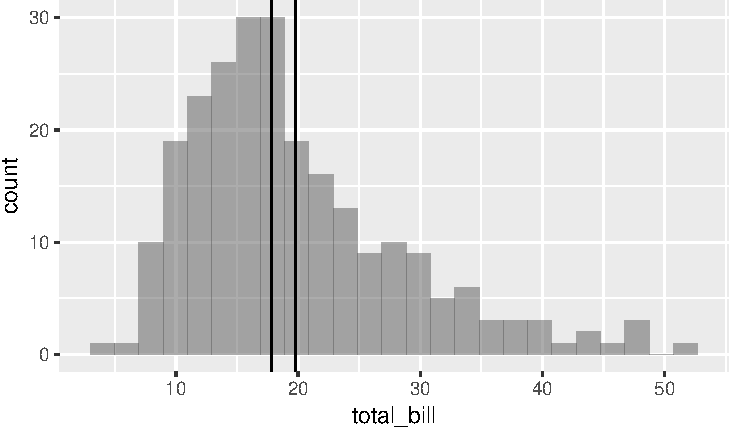
\includegraphics{DatenerhebungStatistik-Uebung_files/figure-latex/unnamed-chunk-61-1.pdf}

Mit Hilfe von
\texttt{\%\textgreater{}\%\ gf\_vline(xintercept\ =\ c(meantb,\ mediantb))}
werden vertikale Linien an den entsprechenden Stellen gezeichnet. Mit
\texttt{gf\_hline(yintercept\ =\ ...)} können horizontale Linien
gezeichnet werden.

\begin{center}\rule{0.5\linewidth}{\linethickness}\end{center}

\textbf{Übung:}

\begin{enumerate}
\def\labelenumi{\arabic{enumi}.}
\setcounter{enumi}{5}
\tightlist
\item
  Begründen Sie anhand des Histogramms, warum hier der Median kleiner
  als der arithmetische Mittelwert ist.
\end{enumerate}

\begin{center}\rule{0.5\linewidth}{\linethickness}\end{center}

Auch Lagemaße zu berechnen in Abhängigkeit der Gruppenzugehörigkeit ist
einfach. So können Sie den arithmetischen Mittelwert in Abhängigkeit von
Geschlecht und Tageszeit berechnen:

\begin{Shaded}
\begin{Highlighting}[]
\KeywordTok{mean}\NormalTok{(total_bill }\OperatorTok{~}\StringTok{ }\NormalTok{sex }\OperatorTok{+}\StringTok{ }\NormalTok{time, }\DataTypeTok{data=}\NormalTok{tips)}
\end{Highlighting}
\end{Shaded}

\begin{verbatim}
## Female.Dinner   Male.Dinner  Female.Lunch    Male.Lunch 
##      19.21308      21.46145      16.33914      18.04848
\end{verbatim}

\begin{center}\rule{0.5\linewidth}{\linethickness}\end{center}

\textbf{Übung:}

\begin{enumerate}
\def\labelenumi{\arabic{enumi}.}
\setcounter{enumi}{6}
\tightlist
\item
  Bestimmen Sie den Median der Trinkgeldhöhe anhand der Anzahl Personen
  in der Tischgesellschaft.
\end{enumerate}

\begin{center}\rule{0.5\linewidth}{\linethickness}\end{center}

Für kategorielle Variablen können eigentlich zunächst nur die
Häufigkeiten bestimmt werden:

\begin{Shaded}
\begin{Highlighting}[]
\KeywordTok{tally}\NormalTok{(}\OperatorTok{~}\NormalTok{day, }\DataTypeTok{data=}\NormalTok{tips)}
\end{Highlighting}
\end{Shaded}

\begin{verbatim}
## day
##  Fri  Sat  Sun Thur 
##   19   87   76   62
\end{verbatim}

Relative Häufigkeiten werden bei \texttt{mosaic} mit der zusätzlichen
Option \texttt{format=\textquotesingle{}proportion\textquotesingle{}}
angefordert:

\begin{Shaded}
\begin{Highlighting}[]
\KeywordTok{tally}\NormalTok{(}\OperatorTok{~}\NormalTok{day, }\DataTypeTok{format=}\StringTok{"proportion"}\NormalTok{, }\DataTypeTok{data=}\NormalTok{tips)}
\end{Highlighting}
\end{Shaded}

\begin{verbatim}
## day
##        Fri        Sat        Sun       Thur 
## 0.07786885 0.35655738 0.31147541 0.25409836
\end{verbatim}

\hypertarget{streuungsmae}{%
\subsection{Streuungsmaße}\label{streuungsmae}}

Die Variation der Daten, die wir grafisch und auch in den (bedingten)
Lagemaßen gesehen haben, ist eines der zentralen Themen der Statistik:
Können wir die Variation vielleicht erklären? Variiert die Rechnungshöhe
vielleicht mit der Anzahl Personen?

Zur Bestimmung der Streuung werden in der Regel der Interquartilsabstand
\texttt{IQR} sowie Varianz \texttt{var} bzw. Standardabweichung
\texttt{sd}
\[s=sd=\sqrt{s^2}=\sqrt{\frac{1}{n-1}\sum_{i=1}^{n}(x_{i}-\bar{x})^2}\]
herangezogen:

\begin{Shaded}
\begin{Highlighting}[]
\KeywordTok{IQR}\NormalTok{(}\OperatorTok{~}\NormalTok{total_bill, }\DataTypeTok{data=}\NormalTok{tips)}
\end{Highlighting}
\end{Shaded}

\begin{verbatim}
## [1] 10.78
\end{verbatim}

\begin{Shaded}
\begin{Highlighting}[]
\KeywordTok{var}\NormalTok{(}\OperatorTok{~}\NormalTok{total_bill, }\DataTypeTok{data=}\NormalTok{tips)}
\end{Highlighting}
\end{Shaded}

\begin{verbatim}
## [1] 79.25294
\end{verbatim}

\begin{Shaded}
\begin{Highlighting}[]
\KeywordTok{sd}\NormalTok{(}\OperatorTok{~}\NormalTok{total_bill, }\DataTypeTok{data=}\NormalTok{tips)}
\end{Highlighting}
\end{Shaded}

\begin{verbatim}
## [1] 8.902412
\end{verbatim}

Um die Standardabweichung in Abhängigkeit der Gruppengröße zu berechnen
genügt der Befehl:

\begin{Shaded}
\begin{Highlighting}[]
\KeywordTok{sd}\NormalTok{(}\OperatorTok{~}\NormalTok{total_bill }\OperatorTok{|}\StringTok{ }\NormalTok{size, }\DataTypeTok{data=}\NormalTok{tips)}
\end{Highlighting}
\end{Shaded}

\begin{verbatim}
##        1        2        3        4        5        6 
## 3.010729 6.043729 9.407065 8.608603 7.340396 9.382000
\end{verbatim}

Bei 4 Personen lag die Standardabweichung als bei 8.61\$.

Um jetzt z. B. den Variationskoeffizienten zu berechnen, wird

\begin{Shaded}
\begin{Highlighting}[]
\KeywordTok{sd}\NormalTok{(}\OperatorTok{~}\NormalTok{total_bill }\OperatorTok{|}\StringTok{ }\NormalTok{size, }\DataTypeTok{data=}\NormalTok{tips) }\OperatorTok{/}\StringTok{ }\KeywordTok{mean}\NormalTok{(}\OperatorTok{~}\NormalTok{total_bill }\OperatorTok{|}\StringTok{ }\NormalTok{size, }\DataTypeTok{data=}\NormalTok{tips)}
\end{Highlighting}
\end{Shaded}

\begin{verbatim}
##         1         2         3         4         5         6 
## 0.4157031 0.3674443 0.4041247 0.3008579 0.2441265 0.2693655
\end{verbatim}

gebildet.

\begin{center}\rule{0.5\linewidth}{\linethickness}\end{center}

\textbf{Übung:}

\begin{enumerate}
\def\labelenumi{\arabic{enumi}.}
\setcounter{enumi}{7}
\tightlist
\item
  Zu welcher Tageszeit ist die Standardabweichung des Trinkgelds
  geringer? Zum Lunch oder zum Dinner?
\end{enumerate}

\begin{center}\rule{0.5\linewidth}{\linethickness}\end{center}

Die \emph{üblichen} deskriptiven Kennzahlen sind in \texttt{mosaic}
übrigens in einer Funktion zusammengefasst: \texttt{favstats}.

\begin{Shaded}
\begin{Highlighting}[]
\KeywordTok{favstats}\NormalTok{(tip}\OperatorTok{~}\NormalTok{day, }\DataTypeTok{data=}\NormalTok{tips)}
\end{Highlighting}
\end{Shaded}

\begin{verbatim}
##    day  min     Q1 median     Q3   max     mean       sd  n missing
## 1  Fri 1.00 1.9600  3.000 3.3650  4.73 2.734737 1.019577 19       0
## 2  Sat 1.00 2.0000  2.750 3.3700 10.00 2.993103 1.631014 87       0
## 3  Sun 1.01 2.0375  3.150 4.0000  6.50 3.255132 1.234880 76       0
## 4 Thur 1.25 2.0000  2.305 3.3625  6.70 2.771452 1.240223 62       0
\end{verbatim}

\hypertarget{zusammenhangsmae}{%
\subsection{Zusammenhangsmaße}\label{zusammenhangsmae}}

Kennzahlen für den linearen Zusammenhang von metrischen Variablen sind
Kovarianz \texttt{cov}
\[s_{xy}=\frac{1}{n-1}\sum_{i=1}^{n}(x_{i}-\bar{x})(y_{i}-\bar{y})\] und
der Korrelationskoeffizient \texttt{cor}
\[r=\frac{\frac{1}{n-1}\sum_{i=1}^{n}(x_{i}-\bar{x})(y_{i}-\bar{y})}{\sqrt{\frac{1}{n-1}\sum_{i=1}^{n}(x_{i}-\bar{x})^2}\sqrt{\frac{1}{n-1}\sum_{i=1}^{n}(y_{i}-\bar{y})^2}}=\frac{s_{xy}}{s_{x}s_{y}}\]

\begin{Shaded}
\begin{Highlighting}[]
\KeywordTok{cov}\NormalTok{(tip }\OperatorTok{~}\StringTok{ }\NormalTok{total_bill, }\DataTypeTok{data=}\NormalTok{tips)}
\end{Highlighting}
\end{Shaded}

\begin{verbatim}
## [1] 8.323502
\end{verbatim}

\begin{Shaded}
\begin{Highlighting}[]
\KeywordTok{cor}\NormalTok{(tip }\OperatorTok{~}\StringTok{ }\NormalTok{total_bill, }\DataTypeTok{data=}\NormalTok{tips)}
\end{Highlighting}
\end{Shaded}

\begin{verbatim}
## [1] 0.6757341
\end{verbatim}

Für kategorielle Variablen wird in diesen Abschnitt zunächst nur die
Kreuztabelle verwendet:

\begin{Shaded}
\begin{Highlighting}[]
\KeywordTok{tally}\NormalTok{(smoker}\OperatorTok{~}\NormalTok{sex, }\DataTypeTok{format=}\StringTok{"proportion"}\NormalTok{, }\DataTypeTok{data=}\NormalTok{tips)}
\end{Highlighting}
\end{Shaded}

\begin{verbatim}
##       sex
## smoker    Female      Male
##    No  0.6206897 0.6178344
##    Yes 0.3793103 0.3821656
\end{verbatim}

\begin{center}\rule{0.5\linewidth}{\linethickness}\end{center}

\textbf{Übung:}

\begin{enumerate}
\def\labelenumi{\arabic{enumi}.}
\setcounter{enumi}{8}
\tightlist
\item
  Zu welcher Tageszeit wurde relativ häufiger von einer Frau die
  Rechnung bezahlt?
\end{enumerate}

\begin{center}\rule{0.5\linewidth}{\linethickness}\end{center}

\hypertarget{ubung-teaching-rating-1}{%
\section{Übung: Teaching Rating}\label{ubung-teaching-rating-1}}

Dieser Datensatz analysiert u. a. den Zusammenhang zwischen Schönheit
und Evaluierungsergebnis von Dozenten:

\emph{Hamermesh, D.S., and Parker, A. (2005). Beauty in the Classroom:
Instructors' Pulchritude and Putative Pedagogical Productivity.
Economics of Education Review, 24, 369--376.}

Sie können ihn von \url{https://goo.gl/6Y3KoK} herunterladen. Anders als
im Paper (und im Paket \texttt{AER}) wird hier nur ein zufälliger Kurs
je Dozent verwendet.

\begin{enumerate}
\def\labelenumi{\arabic{enumi}.}
\tightlist
\item
  Erstellen Sie ein Balkendiagramm der Variable \texttt{native}
  gruppiert nach der Variable \texttt{minority}.
\item
  Erstellen Sie ein Histogramm der Variable \texttt{beauty} gruppiert
  nach der Variable \texttt{gender}.
\item
  Vergleichen Sie das Evaluationsergebnis \texttt{eval} in Abhängigkeit
  ob es sich um einen Single-Credit Kurs \texttt{credits} handelt mit
  Hilfe eines Boxplots.
\item
  Zeichnen Sie ein Scatterplot der Variable \texttt{eval} in
  Abhängigkeit der zu definierenden Variable
  \enquote{Evaluierungsquote}: \texttt{students/allstudents}.
\item
  Berechnen Sie deskriptive Kennzahlen der Variable \texttt{eval} in
  Abhängigkeit ob es sich um einen Single-Credit Kurs \texttt{credits}
  handelt.
\end{enumerate}

\hypertarget{literatur-1}{%
\section{Literatur}\label{literatur-1}}

\begin{itemize}
\tightlist
\item
  David M. Diez, Christopher D. Barr, Mine Çetinkaya-Rundel (2014):
  \emph{Introductory Statistics with Randomization and Simulation},
  \url{https://www.openintro.org/stat/textbook.php?stat_book=isrs},
  Kapitel 1
\item
  Nicholas J. Horton, Randall Pruim, Daniel T. Kaplan (2015):
  \emph{Project MOSAIC Little Books -- A Student's Guide to R},
  \url{https://github.com/ProjectMOSAIC/LittleBooks/raw/master/StudentGuide/MOSAIC-StudentGuide.pdf},
  Kapitel 3.1, 3.2, 4.1, 5.1, 5.2, 6.1
\item
  Chester Ismay, Albert Y. Kim (2017): \emph{ModernDive -- An
  Introduction to Statistical and Data Sciences via R},
  \url{https://ismayc.github.io/moderndiver-book/}
\item
  Maike Luhmann (2015): \emph{R für Einsteiger}, Kapitel 9-11
\item
  Andreas Quatember (2010): \emph{Statistik ohne Angst vor Formeln},
  Kapitel 1
\item
  Daniel Wollschläger (2014): \emph{Grundlagen der Datenanalyse mit R},
  Kapitel 14
\end{itemize}

\hypertarget{lizenz-1}{%
\subsection{Lizenz}\label{lizenz-1}}

Diese Übung wurde von Karsten Lübke entwickelt und orientiert sich an
der Übung zum Buch
\href{https://www.openintro.org/stat/index.php?stat_book=isrs}{OpenIntro}
von Andrew Bray, Mine Çetinkaya-Rundel und Mark Hansen und steht wie
diese unter der Lizenz
\href{http://creativecommons.org/licenses/by-sa/3.0}{Creative Commons
Attribution-ShareAlike 3.0 Unported}. Kleinere Ergänzungen stammen von
Norman Markgraf

\hypertarget{versionshinweise-1}{%
\subsection{Versionshinweise:}\label{versionshinweise-1}}

\begin{itemize}
\tightlist
\item
  Datum erstellt: 2019-01-24
\item
  R Version: 3.5.1
\item
  \texttt{mosaic} Version: 1.4.0
\end{itemize}

\hypertarget{kapitel-2-einfuhrung-wahrscheinlichkeit-und-inferenz}{%
\chapter{Kapitel 2: Einführung Wahrscheinlichkeit und
Inferenz}\label{kapitel-2-einfuhrung-wahrscheinlichkeit-und-inferenz}}

\hypertarget{zufall-und-wahrscheinlichkeit}{%
\section{Zufall und
Wahrscheinlichkeit}\label{zufall-und-wahrscheinlichkeit}}

In dieser Übung werden wir ein wenig programmieren, daher bietet es sich
an, die Befehle in einem Skript zu speichern. Gehen Sie dazu in RStudio
in das Menü \texttt{File} und dort auf \texttt{New\ File} und wählen
\texttt{R\ Script} aus. Dies können Sie dann am Ende über \texttt{File}
und \texttt{Save} bzw. \texttt{Safe\ as} speichern -- und über
\texttt{Open\ File} später auch wieder öffnen. Um die Befehle an die
Konsole zu übergeben klicken Sie entweder auf \texttt{Run} (nur
ausgewählte Zeile, Tastenkürzel \texttt{Strg+Enter}) oder
\texttt{Source} (ganzes Programm).

Zunächst laden wir wieder das Zusatzpaket mosaic, falls noch nicht
geschehen:

\begin{Shaded}
\begin{Highlighting}[]
\KeywordTok{library}\NormalTok{(mosaic)}
\end{Highlighting}
\end{Shaded}

Um den Zufall zu bändigen, setzen wir den Zufallszahlengenerator, z.B.
auf \texttt{1896}

\begin{Shaded}
\begin{Highlighting}[]
\KeywordTok{set.seed}\NormalTok{(}\DecValTok{1896}\NormalTok{)}
\end{Highlighting}
\end{Shaded}

Dieser Befehl sorgt dafür, dass wir immer denselben \enquote{Zufall}
haben.

Beim Roulette gibt es 37 Zahlen und 3 Farben: 0-36, wobei 18 Zahlen
Schwarz, 18 Zahlen Rot und die 0 Grün ist -- auf die Farbe Grün können
Sie auch nicht setzen.

Angenommen Sie setzen auf Farbe. Dann beträgt Ihre
Gewinnwahrscheinlichkeit \(\frac{18}{37}\), da 18 von 37 Fächern
\enquote{ihre} Farbe hat, die Wahrscheinlichkeit eines Verlustes liegt
bei \(\frac{19}{37}=1-\frac{18}{37}\).

Definieren wir in R einen \texttt{factor}-Vektor mit zwei Elementen für
Gewinn und Verlust:

\begin{Shaded}
\begin{Highlighting}[]
\NormalTok{roulette <-}\StringTok{ }\KeywordTok{factor}\NormalTok{(}\KeywordTok{c}\NormalTok{(}\StringTok{"Gewinn"}\NormalTok{, }\StringTok{"Verlust"}\NormalTok{))}
\end{Highlighting}
\end{Shaded}

Mit diesem Vektor können wir jetzt virtuell und ganz ohne Risiko über
den Befehl \texttt{resample} Roulette spielen

\begin{Shaded}
\begin{Highlighting}[]
\KeywordTok{resample}\NormalTok{(roulette, }\DataTypeTok{size=}\DecValTok{1}\NormalTok{, }\DataTypeTok{prob=}\KeywordTok{c}\NormalTok{(}\DecValTok{18}\OperatorTok{/}\DecValTok{37}\NormalTok{, }\DecValTok{19}\OperatorTok{/}\DecValTok{37}\NormalTok{))}
\end{Highlighting}
\end{Shaded}

\begin{verbatim}
## [1] Gewinn
## Levels: Gewinn Verlust
\end{verbatim}

\begin{Shaded}
\begin{Highlighting}[]
\KeywordTok{resample}\NormalTok{(roulette, }\DataTypeTok{size=}\DecValTok{10}\NormalTok{, }\DataTypeTok{prob=}\KeywordTok{c}\NormalTok{(}\DecValTok{18}\OperatorTok{/}\DecValTok{37}\NormalTok{, }\DecValTok{19}\OperatorTok{/}\DecValTok{37}\NormalTok{))}
\end{Highlighting}
\end{Shaded}

\begin{verbatim}
##  [1] Gewinn  Gewinn  Gewinn  Gewinn  Gewinn  Gewinn  Verlust Gewinn 
##  [9] Verlust Gewinn 
## Levels: Gewinn Verlust
\end{verbatim}

Mit dem Argument \texttt{size} wird also eingestellt, wie oft Roulette
gespielt wird, \texttt{prob} ist der Vektor der Wahrscheinlichkeiten für
die einzelnen Elemente im Ereignisvektor, hier \texttt{roulette}.
\texttt{resample} heißt Ziehen mit Zurücklegen.

Über

\begin{Shaded}
\begin{Highlighting}[]
\NormalTok{spiele <-}\StringTok{ }\KeywordTok{resample}\NormalTok{(roulette, }\DataTypeTok{size=}\DecValTok{100}\NormalTok{, }\DataTypeTok{prob=}\KeywordTok{c}\NormalTok{(}\DecValTok{18}\OperatorTok{/}\DecValTok{37}\NormalTok{, }\DecValTok{19}\OperatorTok{/}\DecValTok{37}\NormalTok{))}
\end{Highlighting}
\end{Shaded}

wird dem Vektor \texttt{spiele} das Ergebnis von \texttt{100}
Roulettespielen zugewiesen. Die Häufigkeitsverteilung erhalten wir wie
gewohnt über den Befehl \texttt{tally}:

\begin{Shaded}
\begin{Highlighting}[]
\KeywordTok{tally}\NormalTok{(}\OperatorTok{~}\NormalTok{spiele, }\DataTypeTok{format=}\StringTok{"proportion"}\NormalTok{)}
\end{Highlighting}
\end{Shaded}

\begin{verbatim}
## spiele
##  Gewinn Verlust 
##    0.51    0.49
\end{verbatim}

Das \textbf{Gesetz der großen Zahl} sagt aus, dass sich auf \emph{lange}
Sicht die beobachtete relative Häufigkeit der theoretischen
Wahrscheinlichkeit annähert:

\begin{Shaded}
\begin{Highlighting}[]
\KeywordTok{tally}\NormalTok{(}\OperatorTok{~}\KeywordTok{resample}\NormalTok{(roulette, }\DataTypeTok{size=}\DecValTok{10}\NormalTok{, }\DataTypeTok{prob=}\KeywordTok{c}\NormalTok{(}\DecValTok{18}\OperatorTok{/}\DecValTok{37}\NormalTok{, }\DecValTok{19}\OperatorTok{/}\DecValTok{37}\NormalTok{)), }\DataTypeTok{format=}\StringTok{"proportion"}\NormalTok{)}
\end{Highlighting}
\end{Shaded}

\begin{verbatim}
## resample(roulette, size = 10, prob = c(18/37, 19/37))
##  Gewinn Verlust 
##     0.7     0.3
\end{verbatim}

\begin{Shaded}
\begin{Highlighting}[]
\KeywordTok{tally}\NormalTok{(}\OperatorTok{~}\KeywordTok{resample}\NormalTok{(roulette, }\DataTypeTok{size=}\DecValTok{100}\NormalTok{, }\DataTypeTok{prob=}\KeywordTok{c}\NormalTok{(}\DecValTok{18}\OperatorTok{/}\DecValTok{37}\NormalTok{, }\DecValTok{19}\OperatorTok{/}\DecValTok{37}\NormalTok{)), }\DataTypeTok{format=}\StringTok{"proportion"}\NormalTok{)}
\end{Highlighting}
\end{Shaded}

\begin{verbatim}
## resample(roulette, size = 100, prob = c(18/37, 19/37))
##  Gewinn Verlust 
##    0.44    0.56
\end{verbatim}

\begin{Shaded}
\begin{Highlighting}[]
\KeywordTok{tally}\NormalTok{(}\OperatorTok{~}\KeywordTok{resample}\NormalTok{(roulette, }\DataTypeTok{size=}\DecValTok{1000}\NormalTok{, }\DataTypeTok{prob=}\KeywordTok{c}\NormalTok{(}\DecValTok{18}\OperatorTok{/}\DecValTok{37}\NormalTok{, }\DecValTok{19}\OperatorTok{/}\DecValTok{37}\NormalTok{)), }\DataTypeTok{format=}\StringTok{"proportion"}\NormalTok{)}
\end{Highlighting}
\end{Shaded}

\begin{verbatim}
## resample(roulette, size = 1000, prob = c(18/37, 19/37))
##  Gewinn Verlust 
##   0.488   0.512
\end{verbatim}

\begin{Shaded}
\begin{Highlighting}[]
\KeywordTok{tally}\NormalTok{(}\OperatorTok{~}\KeywordTok{resample}\NormalTok{(roulette, }\DataTypeTok{size=}\DecValTok{1000000}\NormalTok{, }\DataTypeTok{prob=}\KeywordTok{c}\NormalTok{(}\DecValTok{18}\OperatorTok{/}\DecValTok{37}\NormalTok{, }\DecValTok{19}\OperatorTok{/}\DecValTok{37}\NormalTok{)), }\DataTypeTok{format=}\StringTok{"proportion"}\NormalTok{)}
\end{Highlighting}
\end{Shaded}

\begin{verbatim}
## resample(roulette, size = 1e+06, prob = c(18/37, 19/37))
##   Gewinn  Verlust 
## 0.486433 0.513567
\end{verbatim}

Die theoretische Wahrscheinlichkeit eines Gewinns liegt bei
\(\frac{18}{37} \approx 0.4865\): Achtung, das Gesetz der großen Zahl
gilt für den Durchschnitt und auf lange Sicht, evtl. Ungleichgewichte,
z. B. 5 Gewinne in Folge, werden im Laufe der Zeit abgeschwächt und
nicht durch anschließende 5 Verluste ausgeglichen.

Bei bestimmten Spielstrategien, z. B. bei der sogenannten Martingale
oder Verdoppelungsstrategie, ist man daran interessiert, wie
wahrscheinlich es ist, z. B. 8-mal in Folge zu verlieren. Natürlich kann
das mit Hilfe der \emph{Binomialverteilung} ausgerechnet werden, wir
können es aber auch simulieren: \texttt{do()} ist eine einfache
Schleifenfunktion in mosaic. Um z. B. 10000-mal jeweils 8 Runden
Roulette zu spielen -- und das Ergebnis zu speichern -- genügt:

\begin{Shaded}
\begin{Highlighting}[]
\NormalTok{farbspiele <-}\StringTok{ }\KeywordTok{do}\NormalTok{(}\DecValTok{10000}\NormalTok{)}\OperatorTok{*}\KeywordTok{tally}\NormalTok{(}\OperatorTok{~}\KeywordTok{resample}\NormalTok{(roulette, }\DataTypeTok{size =} \DecValTok{8}\NormalTok{, }
                  \DataTypeTok{prob =} \KeywordTok{c}\NormalTok{(}\DecValTok{18}\OperatorTok{/}\DecValTok{37}\NormalTok{, }\DecValTok{19}\OperatorTok{/}\DecValTok{37}\NormalTok{)), }\DataTypeTok{format=}\StringTok{"proportion"}\NormalTok{)}
\end{Highlighting}
\end{Shaded}

\texttt{farbspiele} ist jetzt ein Datensatz (\texttt{data.frame}) mit
10000 Zeilen (=Simulationen) und den relativen Häufigkeiten für Gewinn
und Verlust in den 8 Spielen in den Spalten.

Das Balkendiagramm der relativen Verlusthäufigkeit zeigt, dass es zwar
selten aber doch vorkommt, alle 8 Spiele zu verlieren.

\begin{Shaded}
\begin{Highlighting}[]
\KeywordTok{gf_bar}\NormalTok{(}\OperatorTok{~}\NormalTok{Verlust, }\DataTypeTok{data=}\NormalTok{farbspiele)}
\end{Highlighting}
\end{Shaded}

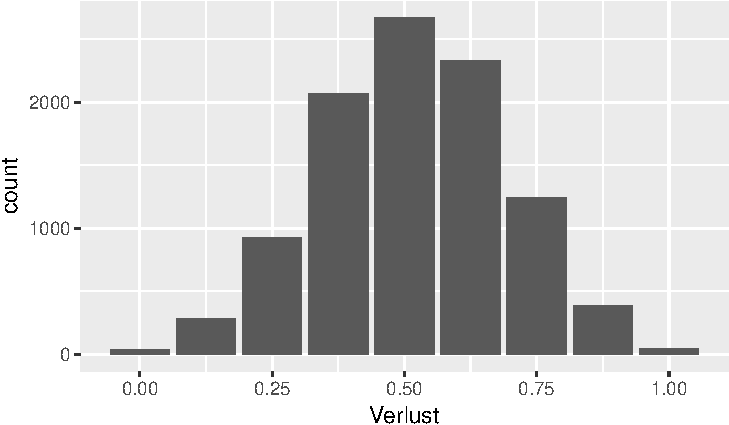
\includegraphics{DatenerhebungStatistik-Uebung_files/figure-latex/unnamed-chunk-79-1.pdf}

Wir haben in 48 von 10000 Wiederholungen nur verloren, d.~h. 8 von 8
Spielen.

\begin{center}\rule{0.5\linewidth}{\linethickness}\end{center}

\textbf{Übung:}

\begin{enumerate}
\def\labelenumi{\arabic{enumi}.}
\tightlist
\item
  Wenn Sie statt auf Farbe auf eine Zahl setzen, beträgt Ihre
  Gewinnwahrscheinlichkeit \(\frac{1}{37}\). Simulieren Sie 10000-mal 10
  Spiele. Wie oft haben Sie mindestens 1-mal gewonnen?
\end{enumerate}

\begin{center}\rule{0.5\linewidth}{\linethickness}\end{center}

Wenn wir uns die Verteilung der Daten der Übung anschauen

\begin{Shaded}
\begin{Highlighting}[]
\NormalTok{zahlspiele <-}\StringTok{ }\KeywordTok{do}\NormalTok{(}\DecValTok{10000}\NormalTok{)}\OperatorTok{*}\KeywordTok{tally}\NormalTok{(}\OperatorTok{~}\KeywordTok{resample}\NormalTok{(roulette, }\DataTypeTok{size =} \DecValTok{10}\NormalTok{, }
                  \DataTypeTok{prob =} \KeywordTok{c}\NormalTok{(}\DecValTok{1}\OperatorTok{/}\DecValTok{37}\NormalTok{, }\DecValTok{36}\OperatorTok{/}\DecValTok{37}\NormalTok{)), }\DataTypeTok{format =} \StringTok{"proportion"}\NormalTok{)}
\KeywordTok{gf_bar}\NormalTok{(}\OperatorTok{~}\NormalTok{Gewinn, }\DataTypeTok{data=}\NormalTok{zahlspiele)}
\end{Highlighting}
\end{Shaded}

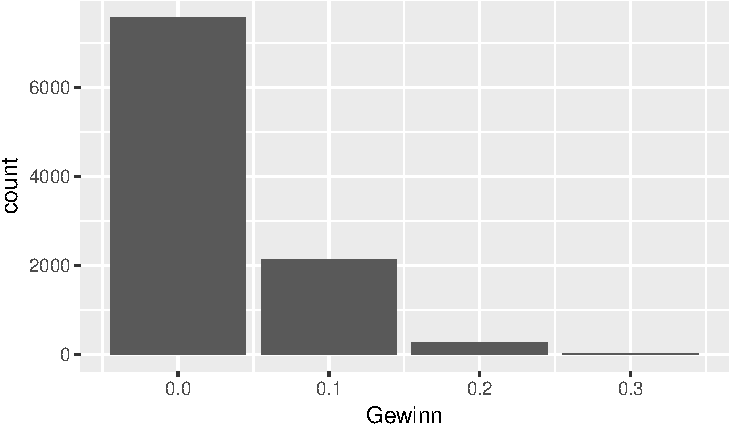
\includegraphics{DatenerhebungStatistik-Uebung_files/figure-latex/unnamed-chunk-80-1.pdf}

stellen wir fest, dass diese Daten (leider) extrem rechtsschief sind,
d.~h., i. d.~R. gewinnen wir in keiner der 10 Runden, Gewinn=0. Wenn wir
\texttt{size=10} durch \texttt{size=1000} ersetzen (d.~h., bei jeden der
10000 Simulationen 1000 Runden spielen), passiert folgendes (Darstellung
jetzt als Histogramm, da es zu sehr viele mögliche Ausprägungen für die
Anzahl Gewinne gibt):

\begin{Shaded}
\begin{Highlighting}[]
\NormalTok{zahlspiele2 <-}\StringTok{ }\KeywordTok{do}\NormalTok{(}\DecValTok{10000}\NormalTok{)}\OperatorTok{*}\KeywordTok{tally}\NormalTok{(}\OperatorTok{~}\KeywordTok{resample}\NormalTok{(roulette, }\DataTypeTok{size =} \DecValTok{1000}\NormalTok{, }
                  \DataTypeTok{prob =} \KeywordTok{c}\NormalTok{(}\DecValTok{1}\OperatorTok{/}\DecValTok{37}\NormalTok{, }\DecValTok{36}\OperatorTok{/}\DecValTok{37}\NormalTok{)), }\DataTypeTok{format =} \StringTok{"proportion"}\NormalTok{)}
\KeywordTok{gf_histogram}\NormalTok{(}\OperatorTok{~}\NormalTok{Gewinn, }\DataTypeTok{data=}\NormalTok{zahlspiele2)}
\end{Highlighting}
\end{Shaded}

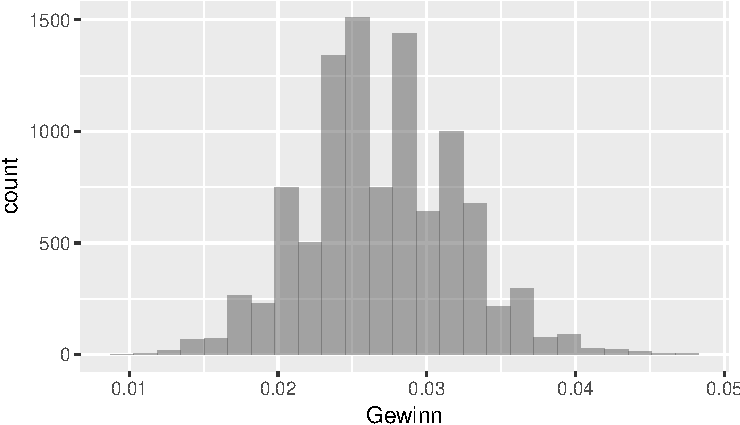
\includegraphics{DatenerhebungStatistik-Uebung_files/figure-latex/unnamed-chunk-81-1.pdf}

Die Daten werden \emph{normaler}, symmetrischer, d.~h., die Verteilung
des Gewinnanteilswertes nähert sich einer Normalverteilung an. Diese
Phänomen ist der Hintergrund des \textbf{Zentralen Grenzwertsatzes}.

\begin{center}\rule{0.5\linewidth}{\linethickness}\end{center}

\textbf{Übung:}

\begin{enumerate}
\def\labelenumi{\arabic{enumi}.}
\setcounter{enumi}{1}
\tightlist
\item
  Zurück zum Farbspiel (\texttt{farbspiele}): Wie hoch schätzen Sie die
  Wahrscheinlichkeit anhand der Simulation, dass Sie mindestens die
  Hälfte Ihrer 8 Spiele gewinnen?
\end{enumerate}

\begin{center}\rule{0.5\linewidth}{\linethickness}\end{center}

Richtig: 0.5994, das ist also anscheinend recht wahrscheinlich, während
der relative Anteil der Spiele, in denen Sie maximal 1 der 8 Spiele
gewinnen, recht klein ist:

\begin{Shaded}
\begin{Highlighting}[]
\NormalTok{anteil <-}\StringTok{ }\KeywordTok{prop}\NormalTok{(farbspiele}\OperatorTok{$}\NormalTok{Gewinn }\OperatorTok{<=}\StringTok{ }\DecValTok{1}\OperatorTok{/}\DecValTok{8}\NormalTok{)}
\NormalTok{anteil}
\end{Highlighting}
\end{Shaded}

Das kommt also eher selten vor. Pech. Vielleicht würden Ihnen aber auch
Zweifel kommen, ob der Tisch fair ist. In der Simulation liegt also die
Wahrscheinlichkeit, bei einem fairen Tisch bei 8 Spielen höchstens
einmal zu gewinnen bei 4.33\(\,\).

\hypertarget{hypothesentest-p-wert-und-konfidenzintervall}{%
\section{Hypothesentest, p-Wert und
Konfidenzintervall}\label{hypothesentest-p-wert-und-konfidenzintervall}}

Im Paper \emph{Hose, C., Lübke, K., Nolte, T., und Obermeier, T. (2012):
Ratingprozess und Ratingergebnis: Ein Experiment bei qualitativen
Ratingkriterien, Kredit \& Rating Praxis (6), 12-14} wird folgendes
Experiment untersucht: Unterscheidet sich die Einschätzung (Rating)
eines Unternehmens, je nach dem, ob die Person alleiniger Entscheider
(Typ A) oder derjenige ist, der die Entscheidungsvorlage vorbereitet
(Typ B). Im Rahmen des Experiments wurden die Studierenden zufällig den
verschiedenen Typen A und B zugeordnet. Von 151 alleinigen Entscheidern
(Typ A) beurteilten 79 das Beispielunternehmen überwiegend positiv (++,
+), von 143 Entscheidungsvorlagenerstellern (Typ B) entschieden
ebenfalls 79 überwiegend positiv.

Zeigt das unterschiedliche Verhältnis: Typ A:
\(\frac{79}{151}=52.32\)\(\,\) zu Typ B: \(\frac{79}{143}=55.24\)\(\,\),
dass alleinige Entscheider die Bonität kritischer einstufen, oder könnte
das Ergebnis Zufall sein?

Das Chancenverhältnis, das \textbf{Odds Ratio} liegt bei
\(\frac{\frac{79}{151-79}}{\frac{79}{143-79}}=0.89\), dass ein
alleiniger Entscheider positiv einstuft -- im Vergleich zum vorläufigen
Entscheider.

Zunächst erzeugen wir einen Vektor der Länge 2 mit den
Entscheidungstypen, aus dem wir simulieren können:

\begin{Shaded}
\begin{Highlighting}[]
\NormalTok{typ <-}\StringTok{ }\KeywordTok{factor}\NormalTok{(}\KeywordTok{c}\NormalTok{(}\StringTok{"A"}\NormalTok{, }\StringTok{"B"}\NormalTok{))}
\NormalTok{entscheider <-}\StringTok{ }\KeywordTok{rep}\NormalTok{(typ, }\KeywordTok{c}\NormalTok{(}\DecValTok{151}\NormalTok{,}\DecValTok{143}\NormalTok{))}
\KeywordTok{tally}\NormalTok{(}\OperatorTok{~}\NormalTok{entscheider)}
\end{Highlighting}
\end{Shaded}

\begin{verbatim}
## entscheider
##   A   B 
## 151 143
\end{verbatim}

sowie einen Vektor der Entscheidungen:

\begin{Shaded}
\begin{Highlighting}[]
\NormalTok{rating <-}\StringTok{ }\KeywordTok{factor}\NormalTok{(}\KeywordTok{c}\NormalTok{(}\StringTok{"Positiv"}\NormalTok{, }\StringTok{"Nicht Positiv"}\NormalTok{))}
\NormalTok{entscheidungen <-}\StringTok{ }\KeywordTok{rep}\NormalTok{(rating, }\KeywordTok{c}\NormalTok{(}\DecValTok{79}\OperatorTok{+}\DecValTok{79}\NormalTok{, (}\DecValTok{151}\OperatorTok{+}\DecValTok{143}\NormalTok{)}\OperatorTok{-}\NormalTok{(}\DecValTok{79}\OperatorTok{+}\DecValTok{79}\NormalTok{)))}
\KeywordTok{tally}\NormalTok{(}\OperatorTok{~}\NormalTok{entscheidungen)}
\end{Highlighting}
\end{Shaded}

\begin{verbatim}
## entscheidungen
## Nicht Positiv       Positiv 
##           136           158
\end{verbatim}

Aus diesem Vektor ziehen wir eine zufällige Stichprobe von 151
Entscheidungen von Typ A.

\begin{Shaded}
\begin{Highlighting}[]
\NormalTok{simentscheidung <-}\StringTok{ }\KeywordTok{sample}\NormalTok{(entscheidungen, }\DataTypeTok{size=}\DecValTok{151}\NormalTok{)}
\KeywordTok{tally}\NormalTok{(}\OperatorTok{~}\NormalTok{simentscheidung)}
\end{Highlighting}
\end{Shaded}

\begin{verbatim}
## simentscheidung
## Nicht Positiv       Positiv 
##            66            85
\end{verbatim}

Hier wären also zufällig 85 der 151 Entscheidungen des Typ A Positiv
gewesen -- wenn es keinen Zusammanhang zwischen Entscheidungstyp und
Ratingentscheidung gibt. \texttt{sample} bedeutet Ziehen ohne
Zurücklegen, d.~h., jeder der Entscheidungen kann nur einmal gezogen
werden.

Wir oft kommt also zufällig heraus, dass höchstens 79 der 151
Entscheidungen des Typs A (alleinige Entscheider) positiv zugeordnet
werden? Simulieren wir das z. B. 10000-mal:

\begin{Shaded}
\begin{Highlighting}[]
\NormalTok{entsim <-}\StringTok{ }\KeywordTok{do}\NormalTok{(}\DecValTok{10000}\NormalTok{)}\OperatorTok{*}\KeywordTok{tally}\NormalTok{(}\OperatorTok{~}\KeywordTok{sample}\NormalTok{(entscheidungen, }\DataTypeTok{size=}\DecValTok{151}\NormalTok{))}
\KeywordTok{prop}\NormalTok{(entsim}\OperatorTok{$}\NormalTok{Positiv}\OperatorTok{<=}\DecValTok{79}\NormalTok{)}
\end{Highlighting}
\end{Shaded}

\begin{verbatim}
## prop_TRUE 
##    0.3512
\end{verbatim}

Unter der \textbf{Nullhyothese}, dass das Ergebnis zufällig war (d.~h.,
es gibt keinen Zusammenhang zwischen Typ und Rating), wurden in der
Simulation in 35.12\(\,\) der Fälle höchstens 79 positive dem Typ A
zufällig zugeordnet. Dieser \textbf{p-Wert} spricht also nicht wirklich
gegen das Zufallsmodell. \emph{Hinweis:} Wir werden in späteren Kapiteln
bessere Methoden kennenlernen, insbesondere auch solche, die alle
Informationen aus den Daten enthalten und sich nicht nur auf einen
Anteilswert beziehen.

Über

\begin{Shaded}
\begin{Highlighting}[]
\NormalTok{typA <-}\StringTok{ }\KeywordTok{rep}\NormalTok{(rating, }\KeywordTok{c}\NormalTok{(}\DecValTok{79}\NormalTok{, }\DecValTok{151-79}\NormalTok{))}
\end{Highlighting}
\end{Shaded}

erzeugen wir uns einen Vektor, der die \(79\) positiven und \(151-79\)
nicht positiven Urteile von Typ A (alleinige Entscheidung) enthält.

\begin{Shaded}
\begin{Highlighting}[]
\KeywordTok{tally}\NormalTok{(}\OperatorTok{~}\StringTok{ }\NormalTok{typA)}
\end{Highlighting}
\end{Shaded}

\begin{verbatim}
## typA
## Nicht Positiv       Positiv 
##            72            79
\end{verbatim}

Wenn wir jetzt diesen Vektor z. B. 10000-mal resampeln:

\begin{Shaded}
\begin{Highlighting}[]
\NormalTok{typAboot <-}\StringTok{ }\KeywordTok{do}\NormalTok{(}\DecValTok{10000}\NormalTok{)}\OperatorTok{*}\KeywordTok{tally}\NormalTok{(}\OperatorTok{~}\KeywordTok{resample}\NormalTok{(typA), }\DataTypeTok{format=}\StringTok{"proportion"}\NormalTok{)}
\end{Highlighting}
\end{Shaded}

erhalten wir 10000 (resampelte) Stichproben, die jeweils einen
zufälligen Stichprobenanteil haben:

\begin{Shaded}
\begin{Highlighting}[]
\CommentTok{# 79/151: Anteil der Originalstichprobe}
\KeywordTok{gf_histogram}\NormalTok{(}\OperatorTok{~}\NormalTok{Positiv, }\DataTypeTok{data=}\NormalTok{typAboot) }\OperatorTok\StringTok{ }\KeywordTok{gf_vline}\NormalTok{( }\DataTypeTok{xintercept=}\DecValTok{79}\OperatorTok{/}\DecValTok{151}\NormalTok{) }
\end{Highlighting}
\end{Shaded}

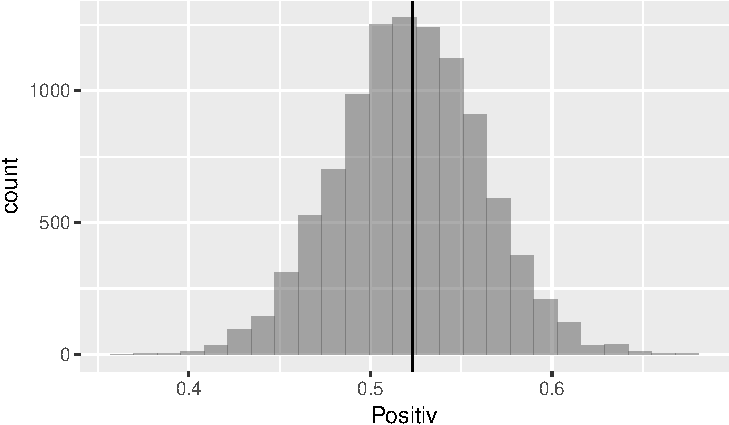
\includegraphics{DatenerhebungStatistik-Uebung_files/figure-latex/unnamed-chunk-90-1.pdf}

In 95\(\,\)\% der Fälle liegt dieser zufällige Stichprobenanteil hier
zwischen

\begin{Shaded}
\begin{Highlighting}[]
\NormalTok{ki <-}\StringTok{ }\KeywordTok{quantile}\NormalTok{(}\OperatorTok{~}\NormalTok{Positiv, }\DataTypeTok{data=}\NormalTok{typAboot, }\DataTypeTok{probs =} \KeywordTok{c}\NormalTok{(}\FloatTok{0.025}\NormalTok{, }\FloatTok{0.975}\NormalTok{))}
\NormalTok{ki}
\end{Highlighting}
\end{Shaded}

\begin{verbatim}
##      2.5%     97.5% 
## 0.4437086 0.6026490
\end{verbatim}

\begin{Shaded}
\begin{Highlighting}[]
\KeywordTok{gf_histogram}\NormalTok{(}\OperatorTok{~}\NormalTok{Positiv, }\DataTypeTok{data=}\NormalTok{typAboot) }\OperatorTok\StringTok{ }\KeywordTok{gf_vline}\NormalTok{(}\DataTypeTok{xintercept=}\NormalTok{ki)}
\end{Highlighting}
\end{Shaded}

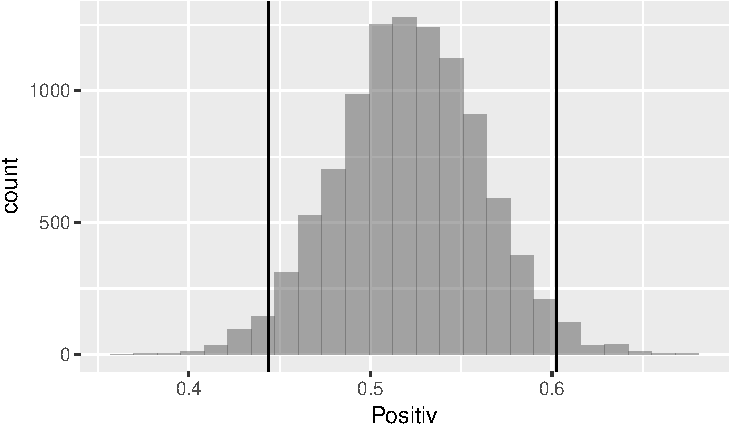
\includegraphics{DatenerhebungStatistik-Uebung_files/figure-latex/unnamed-chunk-91-1.pdf}

Dies ist das \textbf{Nicht-parametrische Bootstrap-Konfidenzintervall}.

\begin{center}\rule{0.5\linewidth}{\linethickness}\end{center}

\textbf{Übung:}

\begin{enumerate}
\def\labelenumi{\arabic{enumi}.}
\setcounter{enumi}{2}
\tightlist
\item
  Bestimmen Sie das 90\(\,\)\% nicht-parametrische
  Bootstrap-Konfidenzintervall für eine nicht-Positive Einschätzung im
  Fall Entscheidungsvorlage (Typ B). Würde damit eine Nullyhpothese
  \(p=0.5\) zum Signifikanzniveau 10\(\,\)\% vermutlich verworfen
  werden?
\end{enumerate}

\begin{center}\rule{0.5\linewidth}{\linethickness}\end{center}

\hypertarget{rechnen-mit-der-normalverteilung}{%
\section{Rechnen mit der
Normalverteilung}\label{rechnen-mit-der-normalverteilung}}

\hypertarget{random-walk}{%
\subsection{Random Walk}\label{random-walk}}

Beim Glücksspiel ist es offensichtlich, aber auch an vielen, vielen
anderen Stellen im Leben begegnen wir dem \emph{Zufall}. Daten,
Beobachtungen sind häufig Realisationen von sogenannten
Zufallsvariablen. Das sind Variablen, deren Werte vom Zufall (und damit
auch seinen Modellen und Gesetzen) abhängen. So werden Aktienkurse und
-renditen häufig als Random Walk aufgefasst und modelliert - häufig
unter der \emph{Annahme} einer Normalverteilung.\footnote{Sowohl die
  Annahme einer Normalverteilung, als auch die Annahme, dass die
  Renditen unabhängig voneinander sind (d.~h., dass keine
  \emph{Autokorrelation} vorliegt) und einer identischen Verteilung
  folgen (hier gleiche Varianz) sind in der Praxis kritisch zu
  hinterfragen.}

Hier drei Kennzahlen der logarithmierten Tagesrenditen von
Aktienunternehmen in 2015 in \%.

\begin{longtable}[]{@{}llll@{}}
\toprule
Anlage & AAPL & FB & GOOGL\tabularnewline
\midrule
\endhead
Mittelwert & -0.08 & 0.11 & 0.15\tabularnewline
Standardabweichung & 1.69 & 1.62 & 1.77\tabularnewline
\bottomrule
\end{longtable}

Unter der Annahme der unabhängig, identischen Normalverteilung der
logarithmierten Renditen können wir jetzt die Wahrscheinlichkeit eines
Tagesverlustes der Apple Aktie (AAPL) berechnen über

\begin{Shaded}
\begin{Highlighting}[]
\KeywordTok{xpnorm}\NormalTok{(}\DecValTok{0}\NormalTok{, }\DataTypeTok{mean=}\OperatorTok{-}\FloatTok{0.08}\NormalTok{, }\DataTypeTok{sd=}\FloatTok{1.69}\NormalTok{ )}
\end{Highlighting}
\end{Shaded}

\begin{verbatim}
## 
\end{verbatim}

\begin{verbatim}
## If X ~ N(-0.08, 1.69), then
\end{verbatim}

\begin{verbatim}
##  P(X <= 0) = P(Z <= 0.04734) = 0.5189
\end{verbatim}

\begin{verbatim}
##  P(X >  0) = P(Z >  0.04734) = 0.4811
\end{verbatim}

\begin{verbatim}
## 
\end{verbatim}

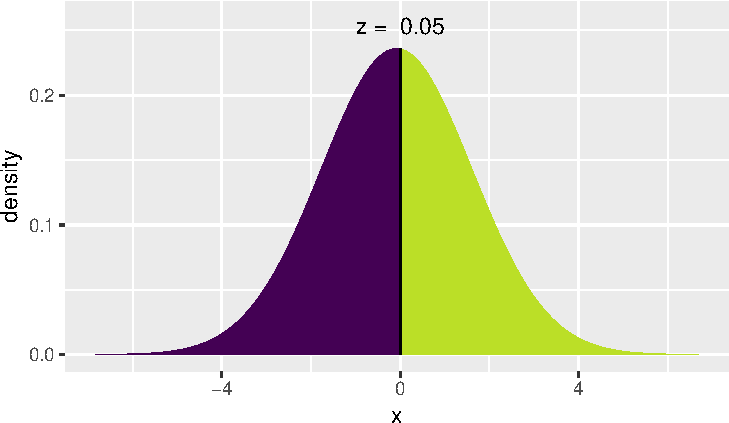
\includegraphics{DatenerhebungStatistik-Uebung_files/figure-latex/unnamed-chunk-92-1.pdf}

\begin{verbatim}
## [1] 0.5188778
\end{verbatim}

Die mosaic Funktion \texttt{xpnorm} ist eine Erweiterung der normalen R
Funktion \texttt{pnorm}, die den Wert der Verteilungsfunktion an einer
gegebenen Stelle zurückgibt -- für jede Verteilung wird hierfür der
vorgestellte Buchstabe \texttt{p} verwendet.

Für Facebook (FB) lag die Wahrscheinlichkeit eines Gewinns demnach bei

\begin{Shaded}
\begin{Highlighting}[]
\KeywordTok{xpnorm}\NormalTok{(}\DecValTok{0}\NormalTok{, }\DataTypeTok{mean=}\FloatTok{0.11}\NormalTok{, }\DataTypeTok{sd=}\FloatTok{1.62}\NormalTok{, }\DataTypeTok{lower.tail =} \OtherTok{FALSE}\NormalTok{)}
\end{Highlighting}
\end{Shaded}

\begin{verbatim}
## 
\end{verbatim}

\begin{verbatim}
## If X ~ N(0.11, 1.62), then
\end{verbatim}

\begin{verbatim}
##  P(X <= 0) = P(Z <= -0.0679) = 0.4729
\end{verbatim}

\begin{verbatim}
##  P(X >  0) = P(Z >  -0.0679) = 0.5271
\end{verbatim}

\begin{verbatim}
## 
\end{verbatim}

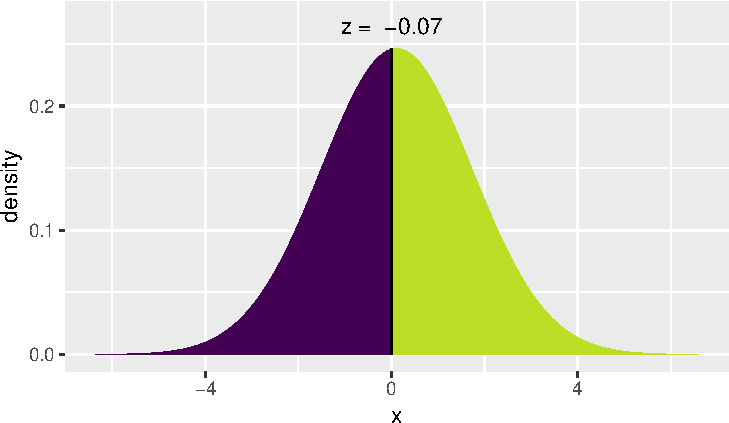
\includegraphics{DatenerhebungStatistik-Uebung_files/figure-latex/unnamed-chunk-93-1.pdf}

\begin{verbatim}
## [1] 0.5270679
\end{verbatim}

Die Voreinstellung ist \texttt{lower.tail\ =\ TRUE}, d.~h., es wird die
Unterschreitungswahrscheinlichkeit angezeigt. Da wir hier aber an der
Überschreitungswahrscheinlichkeit (Gewinn) interessiert sind, muss die
Option auf \texttt{FALSE} gesetzt werden.

\begin{center}\rule{0.5\linewidth}{\linethickness}\end{center}

\textbf{Übung:}

\begin{enumerate}
\def\labelenumi{\arabic{enumi}.}
\setcounter{enumi}{3}
\tightlist
\item
  Welche der drei Aktien hat die höchste Wahrscheinlichkeit eine
  Tagesrendite über 2.5\(\,\)\% zu erzielen?
\end{enumerate}

\begin{center}\rule{0.5\linewidth}{\linethickness}\end{center}

Dabei wird hier immer auch die Z-Transformation, die Standardisierung,
mit angegeben. Am 26.05.2015 (\(r=-2.23\)) betrug der \(z\)-Wert der
Apple Aktie demnach bei

\begin{Shaded}
\begin{Highlighting}[]
\NormalTok{(}\OperatorTok{-}\FloatTok{2.23} \OperatorTok{-}\StringTok{ }\NormalTok{(}\OperatorTok{-}\FloatTok{0.08}\NormalTok{)) }\OperatorTok{/}\StringTok{ }\FloatTok{1.69}
\end{Highlighting}
\end{Shaded}

\begin{verbatim}
## [1] -1.272189
\end{verbatim}

Die Tagesrendite von Apple war also 1.2721893 Standardabweichungen
\emph{unter} dem Mittelwert. Für Facebook lag die Tagesrendite bei
-1.51, der \(z\)-Wert demnach bei:

\begin{Shaded}
\begin{Highlighting}[]
\NormalTok{(}\OperatorTok{-}\FloatTok{1.51} \OperatorTok{-}\StringTok{ }\NormalTok{(}\FloatTok{0.11}\NormalTok{)) }\OperatorTok{/}\StringTok{ }\FloatTok{1.62}
\end{Highlighting}
\end{Shaded}

\begin{verbatim}
## [1] -1
\end{verbatim}

Der 26. Mai 2015 war also auch für Facebook-Anlegerinnen kein guter Tag,
aber immer noch besser als bei Apple.

\begin{center}\rule{0.5\linewidth}{\linethickness}\end{center}

\textbf{Übung:}

\begin{enumerate}
\def\labelenumi{\arabic{enumi}.}
\setcounter{enumi}{4}
\tightlist
\item
  Die Rendite von Google am 26.05.2015 betrug -1.33. Wie hoch ist der
  \(z\)-Wert? Interpretieren Sie die Aussage des Ergebnisses.
\end{enumerate}

\begin{center}\rule{0.5\linewidth}{\linethickness}\end{center}

Wenn wir zu einen gegebenen Wert der Rendite den Wert der
Verteilungsfunktion, d.~h. den prozentualen Anteil kleiner oder gleich
großer Werte suchen (\(P(X \leq x)\)) verwenden wir \texttt{pnorm} bzw.
\texttt{xpnorm}. Wenn die Überschreitungswahrscheinlichkeit (\(P(X>x)\))
gesucht ist, kann zusätzlich die Option \texttt{lower.tail\ =\ TRUE}
gesetzt werden, oder \texttt{1-pnorm()} gerechnet werden.

Um zu einem gegebenen Anteil (Prozentwert) den zugehörigen Wert der
Rendite zu finden, wir also das Quantil suchen, dann wird \texttt{p}
durch \texttt{q} ersetzt, also \texttt{qnorm} bzw. \texttt{xqnorm}.

Z. B. für die 5\(\,\)\% schlechtesten Tage der Appleaktie

\begin{Shaded}
\begin{Highlighting}[]
\KeywordTok{xqnorm}\NormalTok{(}\FloatTok{0.05}\NormalTok{, }\DataTypeTok{mean=}\OperatorTok{-}\FloatTok{0.08}\NormalTok{, }\DataTypeTok{sd=}\FloatTok{1.69}\NormalTok{ )}
\end{Highlighting}
\end{Shaded}

\begin{verbatim}
## 
\end{verbatim}

\begin{verbatim}
## If X ~ N(-0.08, 1.69), then
\end{verbatim}

\begin{verbatim}
##  P(X <= -2.859803) = 0.05
\end{verbatim}

\begin{verbatim}
##  P(X >  -2.859803) = 0.95
\end{verbatim}

\begin{verbatim}
## 
\end{verbatim}

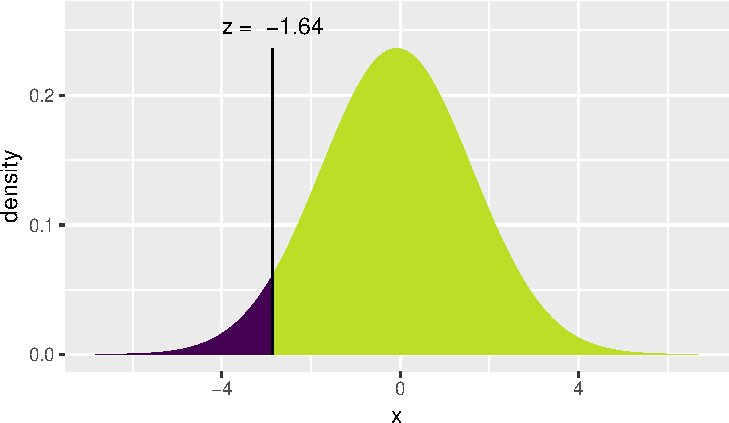
\includegraphics{DatenerhebungStatistik-Uebung_files/figure-latex/unnamed-chunk-96-1.pdf}

\begin{verbatim}
## [1] -2.859803
\end{verbatim}

Die Wahrscheinlichkeit beträgt also \(0,05=5\%\), dass die Tagesrendite
unter -2.86 liegt.

Für die Facebook Aktie gilt, dass Sie nur mit einer Wahrscheinlichkeit
von \(0,01=1\%\) über 3.8786836 lag:

\begin{Shaded}
\begin{Highlighting}[]
\KeywordTok{xqnorm}\NormalTok{(}\FloatTok{0.01}\NormalTok{, }\DataTypeTok{mean=}\FloatTok{0.11}\NormalTok{, }\DataTypeTok{sd=}\FloatTok{1.62}\NormalTok{, }\DataTypeTok{lower.tail =} \OtherTok{FALSE}\NormalTok{)}
\end{Highlighting}
\end{Shaded}

\begin{center}\rule{0.5\linewidth}{\linethickness}\end{center}

\textbf{Übung:}

\begin{enumerate}
\def\labelenumi{\arabic{enumi}.}
\setcounter{enumi}{5}
\tightlist
\item
  Sie wollen Ihre Google-Aktien absichern. Wie groß ist bei einer
  maximalen Eintretenswahrscheinlichkeit von \(1\%\) der Tagesverlust
  mindestens?
\end{enumerate}

\begin{center}\rule{0.5\linewidth}{\linethickness}\end{center}

\hypertarget{ubung-achtsamkeit}{%
\section{Übung: Achtsamkeit}\label{ubung-achtsamkeit}}

In einem Test zur Achtsamkeit \emph{Sauer S, Lemke J, Wittmann M, Kohls
N, Mochty U, and Walach H. (2012) How long is now for mindfulness
meditators? Personality and Individual Differences 52(6), 750--754}
konnten 34 von 38 Studienteilnehmern der Kontrollgruppe nach einer
Instruktion die Dauer der Fixierung des Necker Würfels (Link/Bild)
steigern.

\begin{enumerate}
\def\labelenumi{\arabic{enumi}.}
\tightlist
\item
  Kann diese Verbesserung bei fast 90\(\,\) der Personen zufällig sein?
  Bestimmen Sie mit Hilfe einer Simulation die Wahrscheinlichkeit, dass
  zufällig mindestens 34 von 38 Personen eine Verbesserung erzielen.
\item
  Bestimmen Sie ein nicht-paramatrisches Bootstrap-Konfidenzintervall,
  dass den Anteilswert der Verbesserung in 95\(\,\) der Fälle überdeckt.
\end{enumerate}

\hypertarget{ubung-intelligenzquotient}{%
\section{Übung: Intelligenzquotient}\label{ubung-intelligenzquotient}}

Der IQ hat nach Konstruktion einen arithmetischen Mittelwert von 100 bei
einer Standardabweichung von 15.

\begin{enumerate}
\def\labelenumi{\arabic{enumi}.}
\tightlist
\item
  Wie hoch ist der Anteil der Personen mit einem IQ von 130 oder größer?
\item
  Welchen IQ sollte eine Person mindestens haben, wenn Sie zu den
  1\(\,\) Personen mit dem höchsten IQ gehören will?
\end{enumerate}

\hypertarget{literatur-2}{%
\section{Literatur}\label{literatur-2}}

\begin{itemize}
\tightlist
\item
  David M. Diez, Christopher D. Barr, Mine Çetinkaya-Rundel (2014):
  \emph{Introductory Statistics with Randomization and Simulation},
  \url{https://www.openintro.org/stat/textbook.php?stat_book=isrs},
  Kapitel 2
\item
  Nicholas J. Horton, Randall Pruim, Daniel T. Kaplan (2015): Project
  MOSAIC Little Books \emph{A Student's Guide to R},
  \url{https://github.com/ProjectMOSAIC/LittleBooks/raw/master/StudentGuide/MOSAIC-StudentGuide.pdf},
  Kapitel 3.5, 3.6
\item
  Chester Ismay, Albert Y. Kim (2017): ModernDive -- An Introduction to
  Statistical and Data Sciences via R,
  \url{https://ismayc.github.io/moderndiver-book/}
\item
  Maike Luhmann (2015): \emph{R für Einsteiger}, Kapitel 12
\item
  Andreas Quatember (2010): \emph{Statistik ohne Angst vor Formeln},
  Kapitel 2, 3.1-3.3, 3.13
\item
  Daniel Wollschläger (2014): \emph{Grundlagen der Datenanalyse mit R},
  Kapitel 5, 11
\end{itemize}

\hypertarget{lizenz-2}{%
\subsection{Lizenz}\label{lizenz-2}}

Diese Übung wurde von Karsten Lübke entwickelt und orientiert sich an
der Übung zum Buch
\href{https://www.openintro.org/stat/index.php?stat_book=isrs}{OpenIntro}
von Andrew Bray, Mine Çetinkaya-Rundel und Mark Hansen und steht wie
diese unter der Lizenz
\href{http://creativecommons.org/licenses/by-sa/3.0}{Creative Commons
Attribution-ShareAlike 3.0 Unported}. Kleinere Ergänzungen stammen von
Norman Markgraf

\hypertarget{versionshinweise-2}{%
\subsection{Versionshinweise:}\label{versionshinweise-2}}

\begin{itemize}
\tightlist
\item
  Datum erstellt: 2019-01-24
\item
  R Version: 3.5.1
\item
  \texttt{mosaic} Version: 1.4.0
\end{itemize}

\hypertarget{kapitel-3-einfuhrung-inferenz-kategoriale-werte}{%
\chapter{Kapitel 3: Einführung Inferenz kategoriale
Werte}\label{kapitel-3-einfuhrung-inferenz-kategoriale-werte}}

\hypertarget{globaler-index-der-religiositat-und-atheismus}{%
\section{Globaler Index der Religiösität und
Atheismus}\label{globaler-index-der-religiositat-und-atheismus}}

Im Jahre 2012 führte das \href{http://www.wingia.com/}{WIN/Gallup
International Institut} in 57 Ländern eine Untersuchung zur Religiosität
durch. Die Pressemitteilung zur Studie finden Sie
\href{http://www.wingia.com/web/files/richeditor/filemanager/Global_INDEX_of_Religiosity_and_Atheism_PR__6.pdf}{hier}.

Dabei wurde die Frage gestellt: \emph{Unabhängig davon, ob Sie an
Gottesdiensten teilnehmen oder nicht (\enquote{attend place of
worship}), würden Sie sagen, dass Sie ein religiöser Mensch sind, eine
nicht religiöse Person oder ein überzeugter Atheist?}

Die Befragten hatten dabei drei Antwortmöglichkeiten: Religiöser Mensch
(\enquote{A religious person}), Nicht religiöser Mensch (\enquote{Not a
religious person}), und Atheist (\enquote{A convinced atheist}). Die
Befragten klassifizierten sich, es wurden kategorielle (nominale) Daten
(\texttt{factor}) erzeugt.

\begin{center}\rule{0.5\linewidth}{\linethickness}\end{center}

\textbf{Übung:}

\begin{enumerate}
\def\labelenumi{\arabic{enumi}.}
\tightlist
\item
  Handelt es sich bei den im Bericht angegeben Kennzahlen um
  \emph{Stichprobenstatistiken} oder um \emph{Populationsparameter}?
\item
  Um die Ergebnisse der Studie zu verallgemeinern, also auf die
  Gesamtbevölkerung zu schließen, welche Annahmen müssen dafür erfüllt
  sein und klingen diese hier plausibel erfüllt?
\end{enumerate}

\begin{center}\rule{0.5\linewidth}{\linethickness}\end{center}

Ein Teil der Daten kann direkt von OpenIntro als R Datensatz
heruntergeladen werden, und anschließend in R eingelesen:

\begin{Shaded}
\begin{Highlighting}[]
\NormalTok{meine_url <-}\StringTok{ "http://www.openintro.org/stat/data/atheism.RData"}
\KeywordTok{load}\NormalTok{(}\KeywordTok{url}\NormalTok{(meine_url)) }\CommentTok{# Einlesen}
\end{Highlighting}
\end{Shaded}

Einen Überblick erhält man wie immer über:

\begin{Shaded}
\begin{Highlighting}[]
\KeywordTok{inspect}\NormalTok{(atheism) }\CommentTok{# Datenstruktur}
\end{Highlighting}
\end{Shaded}

\begin{verbatim}
## 
## categorical variables:  
##          name  class levels     n missing
## 1 nationality factor     57 88032       0
## 2    response factor      2 88032       0
##                                    distribution
## 1 Pakistan (6.1%), France (3.8%) ...           
## 2 non-atheist (93.8%), atheist (6.2%)          
## 
## quantitative variables:  
##   name   class  min   Q1 median   Q3  max     mean       sd     n missing
## 1 year integer 2005 2005   2012 2012 2012 2009.129 3.443025 88032       0
\end{verbatim}

\begin{Shaded}
\begin{Highlighting}[]
\KeywordTok{head}\NormalTok{(atheism) }\CommentTok{# Erste Beobachtungen}
\end{Highlighting}
\end{Shaded}

\begin{verbatim}
##   nationality    response year
## 1 Afghanistan non-atheist 2012
## 2 Afghanistan non-atheist 2012
## 3 Afghanistan non-atheist 2012
## 4 Afghanistan non-atheist 2012
## 5 Afghanistan non-atheist 2012
## 6 Afghanistan non-atheist 2012
\end{verbatim}

\begin{Shaded}
\begin{Highlighting}[]
\KeywordTok{tail}\NormalTok{(atheism) }\CommentTok{# letzte Beobachtungen}
\end{Highlighting}
\end{Shaded}

\begin{verbatim}
##       nationality    response year
## 88027     Vietnam non-atheist 2005
## 88028     Vietnam non-atheist 2005
## 88029     Vietnam non-atheist 2005
## 88030     Vietnam non-atheist 2005
## 88031     Vietnam non-atheist 2005
## 88032     Vietnam non-atheist 2005
\end{verbatim}

Hinweis: Die drei Antwortmöglichkeiten wurden im verwendeten Datensatz
zu zwei Leveln (\texttt{atheist}, \texttt{non-atheist}) zusammengefasst.

Zur Analyse wird wieder das Paket mosaic verwendet:

\begin{Shaded}
\begin{Highlighting}[]
\KeywordTok{library}\NormalTok{(mosaic)}
\end{Highlighting}
\end{Shaded}

\hypertarget{inferenz-eines-anteilswerts}{%
\section{Inferenz eines
Anteilswerts}\label{inferenz-eines-anteilswerts}}

In Tabelle 6 der Pressemitteilung wird der Anteil der Atheisten für
Deutschland mit 15\(\,\)\% angegeben. Dies ist eine \emph{Statistik} der
Stichprobe, nicht der Parameter der \emph{Population}. Es wird also die
Frage beantwortet \enquote{Wie hoch ist der Anteil der Atheisten in der
Stichprobe?}. Um die Frage \enquote{Wie hoch ist der Anteil der
Atheisten in der Population?} zu beantworten, muss von der Stichprobe
auf die Population geschlossen werden, d.~h., es wird z. B. der
Anteilswert \emph{geschätzt}.

Der folgende Befehl filtert den Datensatz auf das Ergebnis für
Deutschland im Jahr 2012, d.~h., es werden nur die gewünschten Zeilen im
Datensatz belassen:

\begin{Shaded}
\begin{Highlighting}[]
\NormalTok{de12 <-}\StringTok{ }\KeywordTok{filter}\NormalTok{(atheism, nationality }\OperatorTok{==}\StringTok{ "Germany"}\NormalTok{, year }\OperatorTok{==}\StringTok{ "2012"}\NormalTok{)}
\end{Highlighting}
\end{Shaded}

Die \emph{Punktschätzung} des Anteilswertes der Atheisten für
Deutschland im Jahr 2012 liegt dann bei

\begin{Shaded}
\begin{Highlighting}[]
\NormalTok{pdach <-}\StringTok{ }\KeywordTok{tally}\NormalTok{(}\OperatorTok{~}\NormalTok{response, }\DataTypeTok{data=}\NormalTok{de12, }\DataTypeTok{format=}\StringTok{'proportion'}\NormalTok{)[}\StringTok{"atheist"}\NormalTok{]}
\NormalTok{pdach}
\end{Highlighting}
\end{Shaded}

\begin{verbatim}
##   atheist 
## 0.1494024
\end{verbatim}

also bei 15\(\,\)\%.

Um jetzt ein 95\(\,\)\% Konfidenzintervall für den Populationsparameter
zu konstruieren (\emph{Bereichsschätzung}) muss der Standardfehler
\(se\) bestimmt werden, hier:

\begin{Shaded}
\begin{Highlighting}[]
\NormalTok{n <-}\StringTok{ }\KeywordTok{nrow}\NormalTok{(de12) }\CommentTok{# Anzahl Beobachtungen}
\NormalTok{se <-}\StringTok{ }\KeywordTok{sqrt}\NormalTok{( pdach }\OperatorTok{*}\StringTok{ }\NormalTok{(}\DecValTok{1}\OperatorTok{-}\NormalTok{pdach) }\OperatorTok{/}\StringTok{ }\NormalTok{n)}
\NormalTok{se}
\end{Highlighting}
\end{Shaded}

\begin{verbatim}
##    atheist 
## 0.01591069
\end{verbatim}

Der Standardfehler, d.~h., die Standardabweichung des Anteilswertes
liegt hier also bei 1.59\(\,\)\%. Zusammen mit dem 2,5\(\,\)\% und
97,5\(\,\)\% Quantil der Standardnormalverteilung ergibt sich folgendes
Konfidenzintervall:

\begin{Shaded}
\begin{Highlighting}[]
\NormalTok{pdach }\OperatorTok{+}\StringTok{ }\KeywordTok{qnorm}\NormalTok{(}\KeywordTok{c}\NormalTok{(}\FloatTok{0.025}\NormalTok{, }\FloatTok{0.975}\NormalTok{)) }\OperatorTok{*}\StringTok{ }\NormalTok{se}
\end{Highlighting}
\end{Shaded}

\begin{verbatim}
## [1] 0.1182180 0.1805868
\end{verbatim}

Da der Populationsparameter unbekannt aber nicht zufällig ist, werden
die 95\(\,\)\% auch als \emph{Überdeckungswahrscheinlichkeit}
bezeichnet.

In \texttt{mosaic} besteht die Möglichkeit, Punkt- und
Bereichsschätzungen mit dem Befehl \texttt{prop.test} durchzuführen.
Sofern kein Wert für \texttt{p} angegeben wird lautet die Nullyhpothese
\(H_0: p=0.5\).

\begin{Shaded}
\begin{Highlighting}[]
\KeywordTok{prop.test}\NormalTok{(}\OperatorTok{~}\NormalTok{response, }\DataTypeTok{data=}\NormalTok{de12)}
\end{Highlighting}
\end{Shaded}

\begin{verbatim}
## 
##  1-sample proportions test with continuity correction
## 
## data:  de12$response  [with success = atheist]
## X-squared = 245.42, df = 1, p-value < 2.2e-16
## alternative hypothesis: true p is not equal to 0.5
## 95 percent confidence interval:
##  0.1199815 0.1843172
## sample estimates:
##         p 
## 0.1494024
\end{verbatim}

Beachte, dass das Konfidenzintervall, anders als bei der
\emph{Approximation} über die Normalverteilung hier nicht symmetrisch um
den Punktschätzer ist.

\begin{center}\rule{0.5\linewidth}{\linethickness}\end{center}

\textbf{Übung:}

\begin{enumerate}
\def\labelenumi{\arabic{enumi}.}
\setcounter{enumi}{2}
\tightlist
\item
  Bei annähernd gleicher Stichprobengröße liegt der Anteil der Atheisten
  in Saudi Arabien bei 5\(\,\)\%. Wie verändert sich der Standardfehler
  und damit die Breite des Konfidenzintervalls?
\item
  Der Anteil der Atheisten in Südkorea liegt in etwa ebenfalls bei
  15\(\,\)\%, allerdings liegen die Daten von 1523 Befragten vor. Wie
  verändert sich der Standardfehler und damit die Breite des
  Konfidenzintervalls?
\end{enumerate}

\begin{center}\rule{0.5\linewidth}{\linethickness}\end{center}

Um für Deutschland die Nullhypothese \enquote{Der Anteil der Atheisten
liegt nicht über 10\(\,\)\%} gegen die Alternativhypothese
(Forschungshypothese) \enquote{Der Anteil der Atheisten liegt über
10\(\,\)\%} können entweder wieder Simulations- und Resamplingtechniken
verwendet werden oder die Approximation durch die Normalverteilung:

\begin{Shaded}
\begin{Highlighting}[]
\NormalTok{se0 <-}\StringTok{ }\KeywordTok{sqrt}\NormalTok{( (}\FloatTok{0.1} \OperatorTok{*}\StringTok{ }\NormalTok{(}\DecValTok{1}\FloatTok{-0.1}\NormalTok{)) }\OperatorTok{/}\NormalTok{n)}
\NormalTok{z <-}\StringTok{ }\NormalTok{(pdach }\OperatorTok{-}\StringTok{ }\FloatTok{0.10}\NormalTok{) }\OperatorTok{/}\StringTok{ }\NormalTok{se0}
\KeywordTok{xpnorm}\NormalTok{(z, }\DataTypeTok{lower.tail =} \OtherTok{FALSE}\NormalTok{)}
\end{Highlighting}
\end{Shaded}

\begin{verbatim}
## 
\end{verbatim}

\begin{verbatim}
## If X ~ N(0, 1), then
\end{verbatim}

\begin{verbatim}
##  P(X <= 3.69) = P(Z <= 3.69) = 0.9999
\end{verbatim}

\begin{verbatim}
##  P(X >  3.69) = P(Z >  3.69) = 0.0001123
\end{verbatim}

\begin{verbatim}
## 
\end{verbatim}

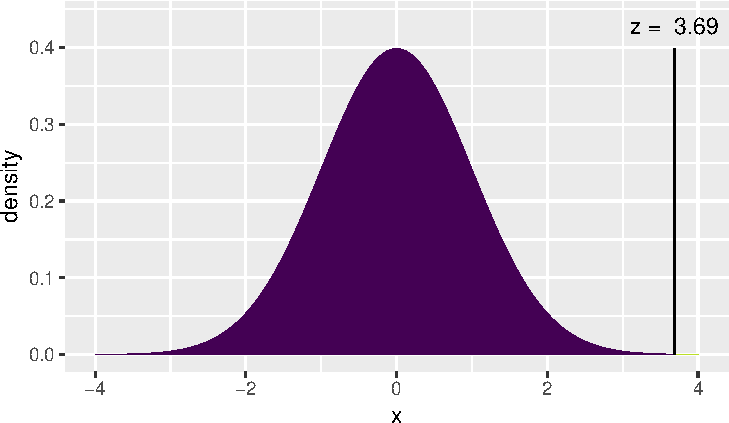
\includegraphics{DatenerhebungStatistik-Uebung_files/figure-latex/unnamed-chunk-106-1.pdf}

\begin{verbatim}
##      atheist 
## 0.0001123062
\end{verbatim}

Der \emph{p-Wert} liegt also bei 0.0112\(\,\)\%, die Nullhypothese wird
also zum Signifikanzniveau von 5\(\,\)\% verworfen.

Auch hier direkt über \texttt{prop.test}:

\begin{Shaded}
\begin{Highlighting}[]
\KeywordTok{prop.test}\NormalTok{(}\OperatorTok{~}\NormalTok{response, }\DataTypeTok{p=}\FloatTok{0.1}\NormalTok{, }\DataTypeTok{alternative=}\StringTok{"greater"}\NormalTok{, }\DataTypeTok{data=}\NormalTok{de12)}
\end{Highlighting}
\end{Shaded}

\begin{verbatim}
## 
##  1-sample proportions test with continuity correction
## 
## data:  de12$response  [with success = atheist]
## X-squared = 13.07, df = 1, p-value = 0.0001501
## alternative hypothesis: true p is greater than 0.1
## 95 percent confidence interval:
##  0.1241944 1.0000000
## sample estimates:
##         p 
## 0.1494024
\end{verbatim}

Je nach Alternativhypothese ergeben sich unterschiedliche Tests:

\begin{itemize}
\tightlist
\item
  \texttt{alternative=\textquotesingle{}two.sided\textquotesingle{}}:
  ungerichtet, d.~h. zweiseitig: \(H_0: p=0.1\) gegen \(H_A: p\neq0.1\)
\item
  \texttt{alternative=\textquotesingle{}less\textquotesingle{}}:
  gerichtet, d.~h. einseitig: \(H_0: p\geq 0.1\) gegen \(H_A: p<0.1\)
\item
  \texttt{alternative=\textquotesingle{}greater\textquotesingle{}}:
  gerichtet, d.~h. einseitig: \(H_0: p\leq 0.1\) gegen \(H_A: p>0.1\)
\end{itemize}

\hypertarget{differenz-zweier-anteilswerte}{%
\section{Differenz zweier
Anteilswerte}\label{differenz-zweier-anteilswerte}}

In den Daten liegen außerdem die Ergebnisse aus 2005 vor:

\begin{Shaded}
\begin{Highlighting}[]
\NormalTok{de05 <-}\StringTok{ }\KeywordTok{filter}\NormalTok{(atheism, nationality }\OperatorTok{==}\StringTok{ "Germany"} \OperatorTok{&}\StringTok{ }\NormalTok{year }\OperatorTok{==}\StringTok{ "2005"}\NormalTok{)}
\end{Highlighting}
\end{Shaded}

Im Jahre 2005 lag der Anteil der Atheisten in Deutschland bei

\begin{Shaded}
\begin{Highlighting}[]
\KeywordTok{tally}\NormalTok{(}\OperatorTok{~}\NormalTok{response, }\DataTypeTok{data=}\NormalTok{de05, }\DataTypeTok{format=}\StringTok{"proportion"}\NormalTok{)}
\end{Highlighting}
\end{Shaded}

\begin{verbatim}
## response
##     atheist non-atheist 
##  0.09960159  0.90039841
\end{verbatim}

Der Aneil lag also bei unter 10\(\,\)\% -- in der \emph{Stichprobe}!
Können wir daraus auf eine Erhöhung des Anteils von 2005 zu 2012 in der
\emph{Population} schließen?

\begin{Shaded}
\begin{Highlighting}[]
\CommentTok{# 2012}
\NormalTok{a12 <-}\StringTok{ }\KeywordTok{tally}\NormalTok{(}\OperatorTok{~}\NormalTok{response, }\DataTypeTok{data=}\NormalTok{de12)[}\StringTok{"atheist"}\NormalTok{] }\CommentTok{# Anzahl Atheisten 2012}
\NormalTok{n12 <-}\StringTok{ }\KeywordTok{nrow}\NormalTok{(de12) }\CommentTok{# Anzahl Studienteilnehmer 2012}
\NormalTok{p12 <-}\StringTok{ }\NormalTok{a12}\OperatorTok{/}\NormalTok{n12 }\CommentTok{# Anteil Atheisten 2012}
\CommentTok{# 2005 }
\NormalTok{a05 <-}\StringTok{ }\KeywordTok{tally}\NormalTok{(}\OperatorTok{~}\NormalTok{response, }\DataTypeTok{data=}\NormalTok{de05)[}\StringTok{"atheist"}\NormalTok{] }\CommentTok{# Anzahl Atheisten 2005}
\NormalTok{n05 <-}\StringTok{ }\KeywordTok{nrow}\NormalTok{(de05) }\CommentTok{# Anzahl Studienteilnehmer 2005}
\NormalTok{p05 <-}\StringTok{ }\NormalTok{a05}\OperatorTok{/}\NormalTok{n05 }\CommentTok{# Anteil Atheisten 2005}
\CommentTok{# Punktschätzer Differenz Population}
\NormalTok{pdiff <-}\StringTok{ }\NormalTok{p12 }\OperatorTok{-}\StringTok{ }\NormalTok{p05}
\NormalTok{pdiff}
\end{Highlighting}
\end{Shaded}

\begin{verbatim}
##   atheist 
## 0.0498008
\end{verbatim}

\begin{Shaded}
\begin{Highlighting}[]
\CommentTok{# Pooling zur Berechnung Standardfehler unter H_0}
\NormalTok{ppool <-}\StringTok{ }\NormalTok{(a12 }\OperatorTok{+}\StringTok{ }\NormalTok{a05)}\OperatorTok{/}\NormalTok{(n12 }\OperatorTok{+}\StringTok{ }\NormalTok{n05)}
\NormalTok{ppool}
\end{Highlighting}
\end{Shaded}

\begin{verbatim}
##  atheist 
## 0.124502
\end{verbatim}

\begin{Shaded}
\begin{Highlighting}[]
\CommentTok{# Standardfehler se}
\NormalTok{se0 <-}\StringTok{ }\KeywordTok{sqrt}\NormalTok{( (ppool }\OperatorTok{*}\StringTok{ }\NormalTok{(}\DecValTok{1} \OperatorTok{-}\StringTok{ }\NormalTok{ppool) }\OperatorTok{/}\StringTok{ }\NormalTok{n12) }\OperatorTok{+}\StringTok{ }\NormalTok{(ppool }\OperatorTok{*}\StringTok{ }\NormalTok{(}\DecValTok{1} \OperatorTok{-}\StringTok{ }\NormalTok{ppool) }\OperatorTok{/}\StringTok{ }\NormalTok{n05) )}
\NormalTok{se0}
\end{Highlighting}
\end{Shaded}

\begin{verbatim}
##   atheist 
## 0.0208391
\end{verbatim}

\begin{Shaded}
\begin{Highlighting}[]
\CommentTok{# z-Wert z}
\NormalTok{z <-}\StringTok{ }\NormalTok{(pdiff }\OperatorTok{-}\StringTok{ }\DecValTok{0}\NormalTok{)}\OperatorTok{/}\NormalTok{se0}
\CommentTok{# p-Wert}
\KeywordTok{xpnorm}\NormalTok{(z, }\DataTypeTok{lower.tail =} \OtherTok{FALSE}\NormalTok{)}
\end{Highlighting}
\end{Shaded}

\begin{verbatim}
## 
\end{verbatim}

\begin{verbatim}
## If X ~ N(0, 1), then
\end{verbatim}

\begin{verbatim}
##  P(X <= 2.39) = P(Z <= 2.39) = 0.9916
\end{verbatim}

\begin{verbatim}
##  P(X >  2.39) = P(Z >  2.39) = 0.008429
\end{verbatim}

\begin{verbatim}
## 
\end{verbatim}

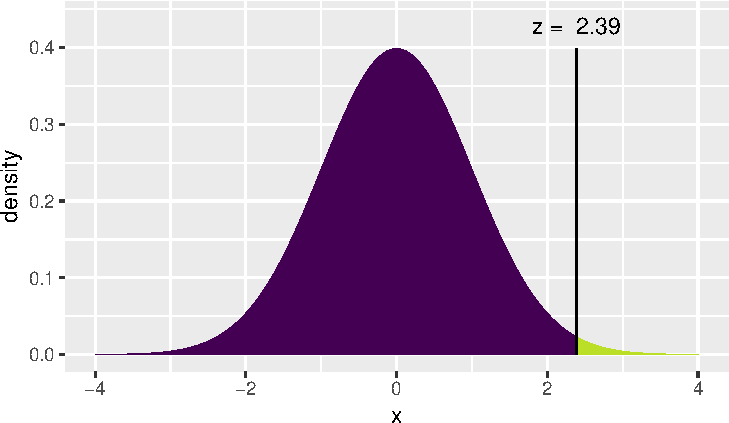
\includegraphics{DatenerhebungStatistik-Uebung_files/figure-latex/unnamed-chunk-110-1.pdf}

\begin{verbatim}
##     atheist 
## 0.008429297
\end{verbatim}

Der p-Wert ist klein und das Ergebnis damit \emph{statistisch
signifikant}. Die Wahrscheinlichkeit, \emph{zufällig} eine solche
Erhöhung der Anteilswerte zu beobachten, ist also gering -- wenn die
\(H_0\) gilt! D. h., es wird auf eine Veränderung des Anteilswertes in
der \emph{Population} geschlossen.

Auch dies kann direkt durch den Befehl \texttt{prop.test} gestestet
werden. Dazu wird zunächst ein gemeinsamer Datensatz erzeugt:

\begin{Shaded}
\begin{Highlighting}[]
\NormalTok{de <-}\StringTok{ }\KeywordTok{filter}\NormalTok{(atheism, nationality }\OperatorTok{==}\StringTok{ "Germany"}\NormalTok{)}
\end{Highlighting}
\end{Shaded}

und anschließend geteset:

\begin{Shaded}
\begin{Highlighting}[]
\KeywordTok{prop.test}\NormalTok{(response}\OperatorTok{~}\NormalTok{year, }\DataTypeTok{alternative=}\StringTok{"less"}\NormalTok{, }\DataTypeTok{data=}\NormalTok{de)}
\end{Highlighting}
\end{Shaded}

\begin{verbatim}
## 
##  2-sample test for equality of proportions with continuity
##  correction
## 
## data:  tally(response ~ year)
## X-squared = 5.2633, df = 1, p-value = 0.01089
## alternative hypothesis: less
## 95 percent confidence interval:
##  -1.00000000 -0.01362913
## sample estimates:
##     prop 1     prop 2 
## 0.09960159 0.14940239
\end{verbatim}

Hier wird die Alternativhypothese \texttt{less} verwendet:
\(H_0: p_1 \geq p_2\), gegen \(H_A: p_1<p_2\).

\emph{Exkurs:} Mit dem Paket mosaic können Sie das auch einfach über
Permutationen testen, indem das Erhebungsjahr zufällig gesampelt wird,
wobei hier ungerichtet, d.~h., zweiseitig getestet wird. Mit anderen
Worten ist sowohl eine Erhöhung als auch ein Verringerung des Anteils in
der Alternativhypothese möglich, daher werden die Absolutwerte der
Differenz (\texttt{abs()}) verwendet:

\begin{Shaded}
\begin{Highlighting}[]
\CommentTok{# Beobachtete Differenz}
\NormalTok{pdiff <-}\StringTok{ }\KeywordTok{diffprop}\NormalTok{( }\OperatorTok{~}\StringTok{ }\NormalTok{response }\OperatorTok{|}\StringTok{ }\NormalTok{year, }\DataTypeTok{data =}\NormalTok{ de)}
\NormalTok{pdiff}
\end{Highlighting}
\end{Shaded}

\begin{verbatim}
##  diffprop 
## 0.0498008
\end{verbatim}

\begin{Shaded}
\begin{Highlighting}[]
\CommentTok{# Zufallszahlengenerator setzen (Reproduzierbarkeit!)}
\KeywordTok{set.seed}\NormalTok{(}\DecValTok{1896}\NormalTok{)}
\CommentTok{# 10000-mal das Jahr permutieren: Nullhypothese kein Unterschied}
\NormalTok{pdiff.null <-}\StringTok{ }\KeywordTok{do}\NormalTok{(}\DecValTok{10000}\NormalTok{) }\OperatorTok{*}\StringTok{ }\KeywordTok{diffprop}\NormalTok{( }\OperatorTok{~}\StringTok{ }\NormalTok{response }\OperatorTok{|}\StringTok{ }\KeywordTok{shuffle}\NormalTok{(year), }\DataTypeTok{data =}\NormalTok{ de)}
\CommentTok{# Histogramm}
\KeywordTok{histogram}\NormalTok{(}\OperatorTok{~}\StringTok{ }\NormalTok{diffprop, }\DataTypeTok{data =}\NormalTok{ pdiff.null, }\DataTypeTok{v =} \KeywordTok{c}\NormalTok{(pdiff, }\OperatorTok{-}\NormalTok{pdiff))}
\end{Highlighting}
\end{Shaded}

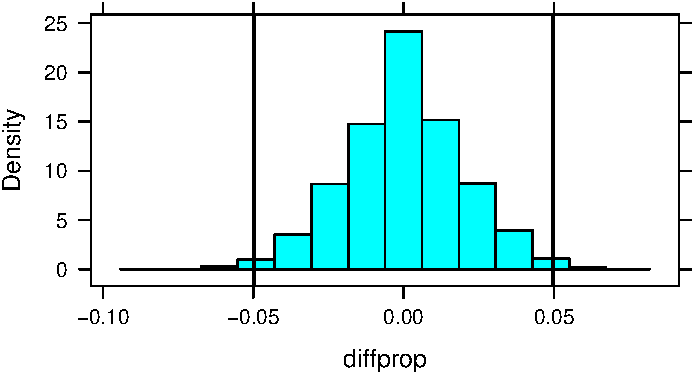
\includegraphics{DatenerhebungStatistik-Uebung_files/figure-latex/unnamed-chunk-113-1.pdf}

\begin{Shaded}
\begin{Highlighting}[]
\CommentTok{# p-Wert}
\KeywordTok{prop}\NormalTok{(}\OperatorTok{~}\KeywordTok{abs}\NormalTok{(diffprop) }\OperatorTok{>=}\StringTok{ }\KeywordTok{abs}\NormalTok{(pdiff), }\DataTypeTok{data =}\NormalTok{ pdiff.null)}
\end{Highlighting}
\end{Shaded}

\begin{verbatim}
## prop_TRUE 
##    0.0192
\end{verbatim}

\begin{center}\rule{0.5\linewidth}{\linethickness}\end{center}

\textbf{Übung:}

\begin{enumerate}
\def\labelenumi{\arabic{enumi}.}
\setcounter{enumi}{4}
\tightlist
\item
  Überprüfen Sie für das Jahr 2012, ob es eine zum Niveau 5\(\,\)\%
  signifikante Differenz zwischen den Anteil der Atheisten in
  Deutschland und den Niederlanden (\texttt{Netherlands}) in der
  Population gibt.
\item
  Überprüfen Sie für das Jahr 2012, ob es eine zum Niveau 5\(\,\)\%
  signifikante Differenz zwischen den Anteil der Atheisten in
  Deutschland und Polen (\texttt{Poland}) in der Population gibt.
\end{enumerate}

\begin{center}\rule{0.5\linewidth}{\linethickness}\end{center}

\hypertarget{chi-quadrat-unabhangigkeitstest}{%
\section{Chi-Quadrat
Unabhängigkeitstest}\label{chi-quadrat-unabhangigkeitstest}}

Soll allgemein der Zusammenhang zwischen zwei kategoriellen (nominalen)
Variablen untersucht werden, wird der
Chi\textsuperscript{2}-Unabhängigkeitstest verwendet. Diese testet die
Nullhypothese der Unabhängigkeit gegen die Alternativhypothese des
Zusammenhangs. Im vorliegenden Datensatz können wir z.B. testen, ob die
Verteilung (Anteil) der Atheisten in den teilnehmenden G7 Ländern gleich
ist:

\begin{Shaded}
\begin{Highlighting}[]
\NormalTok{G7 <-}\StringTok{ }\KeywordTok{c}\NormalTok{(}\StringTok{"United States"}\NormalTok{, }\StringTok{"Canada"}\NormalTok{, }\StringTok{"Germany"}\NormalTok{, }\StringTok{"France"}\NormalTok{, }\StringTok{"Italy"}\NormalTok{, }\StringTok{"Japan"}\NormalTok{)}
\NormalTok{G7}\FloatTok{.12}\NormalTok{ <-}\StringTok{ }\KeywordTok{filter}\NormalTok{(atheism, nationality }\OperatorTok\StringTok{ }\NormalTok{G7 }\OperatorTok{&}\StringTok{ }\NormalTok{year }\OperatorTok{==}\StringTok{ }\DecValTok{2012}\NormalTok{)}
\NormalTok{G7}\FloatTok{.12}\NormalTok{ <-}\StringTok{ }\KeywordTok{droplevels}\NormalTok{(G7}\FloatTok{.12}\NormalTok{)}
\NormalTok{G7atheist <-}\StringTok{ }\KeywordTok{tally}\NormalTok{(response }\OperatorTok{~}\StringTok{ }\NormalTok{nationality, }\DataTypeTok{data =}\NormalTok{ G7}\FloatTok{.12}\NormalTok{)}
\NormalTok{G7atheist}
\end{Highlighting}
\end{Shaded}

\begin{verbatim}
##              nationality
## response      Canada France Germany Italy Japan United States
##   atheist         90    485      75    79   372            50
##   non-atheist    912   1203     427   908   840           952
\end{verbatim}

(Der Befehl \texttt{droplevels} sorgt dafür, dass die nicht mehr
benötigten Ausprägungen der kategoriellen Variablen (\texttt{factor})
gelöscht werden.)

Der Test selber erfolgt in mosaic über \texttt{xchisq.test}, d.~h.:

\begin{Shaded}
\begin{Highlighting}[]
\KeywordTok{xchisq.test}\NormalTok{(G7atheist)}
\end{Highlighting}
\end{Shaded}

\begin{verbatim}
## 
##  Pearson's Chi-squared test
## 
## data:  x
## X-squared = 504.04, df = 5, p-value < 2.2e-16
## 
##     90      485       75       79      372       50  
## ( 180.40) ( 303.91) (  90.38) ( 177.70) ( 218.21) ( 180.40)
## [ 45.30] [107.91] [  2.62] [ 54.82] [108.39] [ 94.26]
## <-6.73>  <10.39>  <-1.62>  <-7.40>  <10.41>  <-9.71> 
##            
##    912     1203      427      908      840      952  
## ( 821.60) (1384.09) ( 411.62) ( 809.30) ( 993.79) ( 821.60)
## [  9.95] [ 23.69] [  0.57] [ 12.04] [ 23.80] [ 20.70]
## < 3.15>  <-4.87>  < 0.76>  < 3.47>  <-4.88>  < 4.55> 
##            
## key:
##  observed
##  (expected)
##  [contribution to X-squared]
##  <Pearson residual>
\end{verbatim}

Der Wert der Teststatistik Chi\textsuperscript{2} liegt bei 504.04, die
Anzahl der Freiheitsgrade (\enquote{degrees of freedom}, df) bei 5, der
p-Wert ist sehr klein, die Nullhypothese der Unabhängigkeit von
Nationalität und Verteilung Atheismus wird für die \emph{Population}
verworfen.

Die Formel zur Berechnung der \(\chi^2\) Teststatistik lautet:
\[\chi^2=\sum_{i=1}^{k}\sum_{j=1}^{m}\frac{(h_{ij}-e_{ij})^{2}}{e_{ij}}\]
mit den erwarteten Häufigkeiten
\(e_{ij}=\frac{h_{i\cdot}h_{\cdot j}}{n}\) wobei für die Zeilensumme
\(h_{i\cdot}=\sum_{j=1}^{m}h_{ij}\) und für die Spaltensumme
\(h_{\cdot j}=\sum_{i=1}^{k}h_{ij}\) gilt.

Mit diesen Daten kann auch über den Befehl \texttt{pchisq} der p-Wert
berechnet werden:

\begin{Shaded}
\begin{Highlighting}[]
\KeywordTok{pchisq}\NormalTok{(}\DecValTok{504}\NormalTok{, }\DecValTok{5}\NormalTok{, }\DataTypeTok{lower.tail =} \OtherTok{FALSE}\NormalTok{)}
\end{Highlighting}
\end{Shaded}

\begin{verbatim}
## [1] 1.093548e-106
\end{verbatim}

\begin{center}\rule{0.5\linewidth}{\linethickness}\end{center}

\textbf{Übung:}

\begin{enumerate}
\def\labelenumi{\arabic{enumi}.}
\setcounter{enumi}{6}
\tightlist
\item
  Gibt es einen Zusammenhang zwischen der Verteilung des Atheismus und
  der Nationalität im Jahr 2012 innerhalb der afrikanischen Länder
  \texttt{c(\textquotesingle{}Nigeria\textquotesingle{},\textquotesingle{}Kenya\textquotesingle{},\ \textquotesingle{}Tunisia\textquotesingle{},\ \textquotesingle{}Ghana\textquotesingle{},\ \textquotesingle{}Cameroon\textquotesingle{},\ \textquotesingle{}South\ Sudan\textquotesingle{})}?
\end{enumerate}

\begin{center}\rule{0.5\linewidth}{\linethickness}\end{center}

\hypertarget{ubung-trinkgelddaten}{%
\section{Übung: Trinkgelddaten}\label{ubung-trinkgelddaten}}

Wir werden jetzt den \emph{tips} Datensatz aus \emph{Bryant, P. G. and
Smith, M (1995) Practical Data Analysis: Case Studies in Business
Statistics. Homewood, IL: Richard D. Irwin Publishing} weiter
analysieren.

Sofern noch nicht geschehen, können Sie diesen als \texttt{csv} Datei
herunterladen:

\begin{Shaded}
\begin{Highlighting}[]
\KeywordTok{download.file}\NormalTok{(}\StringTok{"https://goo.gl/whKjnl"}\NormalTok{, }\DataTypeTok{destfile =} \StringTok{"tips.csv"}\NormalTok{)}
\end{Highlighting}
\end{Shaded}

Das Einlesen erfolgt, sofern die Daten im aktuellen Verzeichnis liegen,
über:

\begin{Shaded}
\begin{Highlighting}[]
\NormalTok{tips <-}\StringTok{ }\KeywordTok{read.csv2}\NormalTok{(}\StringTok{"tips.csv"}\NormalTok{)}
\end{Highlighting}
\end{Shaded}

\emph{Tipp:} Wenn Sie nicht mehr wissen wo die Daten liegen: statt
\texttt{tips.csv} den Befehl \texttt{file.choose()} als Argument für die
Funktion \texttt{read.csv2} verwenden.

\begin{enumerate}
\def\labelenumi{\arabic{enumi}.}
\tightlist
\item
  Bestimmen Sie ein 90\(\,\)\% Konfidenzintervall für den Anteil der
  Raucher (\texttt{smoker}) in der Population.
\item
  Testen Sie zum Niveau 5\(\,\)\%, ob sich der Anteil der Raucher in der
  Population beim Lunch von dem beim Dinner (\texttt{time})
  unterscheidet.
\item
  Gibt es einen Zusammenhang zwischen Rauchen und Wochentag
  (\texttt{day})?
\end{enumerate}

\hypertarget{literatur-3}{%
\section{Literatur}\label{literatur-3}}

\begin{itemize}
\tightlist
\item
  David M. Diez, Christopher D. Barr, Mine Çetinkaya-Rundel (2014):
  \emph{Introductory Statistics with Randomization and Simulation},
  \url{https://www.openintro.org/stat/textbook.php?stat_book=isrs},
  Kapitel 3
\item
  Nicholas J. Horton, Randall Pruim, Daniel T. Kaplan (2015): Project
  MOSAIC Little Books \emph{A Student's Guide to R},
  \url{https://github.com/ProjectMOSAIC/LittleBooks/raw/master/StudentGuide/MOSAIC-StudentGuide.pdf},
  Kapitel 4.2, 4.3, 6.3
\item
  Maike Luhmann (2015): \emph{R für Einsteiger}, Kapitel 18.1
\item
  Andreas Quatember (2010): \emph{Statistik ohne Angst vor Formeln},
  Kapitel 3.4, 3.6, 3.8
\item
  Daniel Wollschläger (2014): \emph{Grundlagen der Datenanalyse mit R},
  Kapitel 10.2
\end{itemize}

\hypertarget{lizenz-3}{%
\subsection{Lizenz}\label{lizenz-3}}

Diese Übung wurde von Karsten Lübke entwickelt und orientiert sich an
der Übung zum Buch
\href{https://www.openintro.org/stat/index.php?stat_book=isrs}{OpenIntro}
von Andrew Bray, Mine Çetinkaya-Rundel und steht wie diese unter der
Lizenz \href{http://creativecommons.org/licenses/by-sa/3.0}{Creative
Commons Attribution-ShareAlike 3.0 Unported}.

\hypertarget{versionshinweise-3}{%
\subsection{Versionshinweise:}\label{versionshinweise-3}}

\begin{itemize}
\tightlist
\item
  Datum erstellt: 2019-01-24
\item
  R Version: 3.5.1
\item
  \texttt{mosaic} Version: 1.4.0
\end{itemize}

\hypertarget{kapitel-4-einfuhrung-inferenz-metrische-werte}{%
\chapter{Kapitel 4: Einführung Inferenz metrische
Werte}\label{kapitel-4-einfuhrung-inferenz-metrische-werte}}

\hypertarget{t-test-fur-eine-stichprobe}{%
\section{t-Test für eine Stichprobe}\label{t-test-fur-eine-stichprobe}}

Der B3 Datensatz \emph{Heilemann, U. and Münch, H.J. (1996): West German
Business Cycles 1963-1994: A Multivariate Discriminant Analysis.
CIRET--Conference in Singapore, CIRET--Studien 50.} enthält
Quartalsweise Konjunkturdaten aus (West-)Deutschland von 1955-1994.

Er kann von \url{https://goo.gl/0YCEHf} heruntergeladen werden:

\begin{Shaded}
\begin{Highlighting}[]
\KeywordTok{download.file}\NormalTok{(}\StringTok{"https://goo.gl/0YCEHf"}\NormalTok{, }\DataTypeTok{destfile =} \StringTok{"B3.csv"}\NormalTok{)}
\end{Highlighting}
\end{Shaded}

Anschließend können die Daten in R eingelesen werden:

\begin{Shaded}
\begin{Highlighting}[]
\NormalTok{B3 <-}\StringTok{ }\KeywordTok{read.csv2}\NormalTok{(}\StringTok{"B3.csv"}\NormalTok{)}
\KeywordTok{str}\NormalTok{(B3) }\CommentTok{# Datenstruktur}
\end{Highlighting}
\end{Shaded}

\begin{verbatim}
## 'data.frame':    157 obs. of  14 variables:
##  $ PHASEN  : int  2 2 3 3 3 3 3 3 3 3 ...
##  $ BSP91JW : num  10.53 10.6 9.21 5.17 4.93 ...
##  $ CP91JW  : num  9.31 12.66 6.55 7.87 8.6 ...
##  $ DEFRATE : num  0.05 0.06 0.05 0.05 0.04 0.04 0.04 0.03 0.03 0 ...
##  $ EWAJW   : num  5.7 5.2 4.8 3.3 2.1 3.2 2.5 2.7 3 0.3 ...
##  $ EXIMRATE: num  3.08 1.96 2.82 3.74 4.16 2.9 3.65 4.57 4.37 2.89 ...
##  $ GM1JW   : num  11.15 11.03 10.04 8.33 7.69 ...
##  $ IAU91JW : num  23.56 12.72 11.52 0.85 -2.08 ...
##  $ IB91JW  : num  14.69 24.95 14.9 7.55 3.23 ...
##  $ LSTKJW  : num  3 2.36 3.39 5.3 6.91 1.03 3.73 6.2 4.12 7.94 ...
##  $ PBSPJW  : num  2.89 2.59 3.01 3.03 3.46 1.95 3.18 3.98 3.29 5.63 ...
##  $ PCPJW   : num  1.91 2.2 3.09 2.08 1.48 1.65 1.47 3.29 3.59 4.19 ...
##  $ ZINSK   : num  6.27 4.6 6.19 6.71 7.1 4.96 5.21 4.83 4.5 3.83 ...
##  $ ZINSLR  : num  3.21 3.54 3.22 3.37 3.14 4.95 3.82 3.09 3.91 1.47 ...
\end{verbatim}

\begin{Shaded}
\begin{Highlighting}[]
\KeywordTok{head}\NormalTok{(B3); }\KeywordTok{tail}\NormalTok{(B3)}
\end{Highlighting}
\end{Shaded}

\begin{verbatim}
##   PHASEN BSP91JW CP91JW DEFRATE EWAJW EXIMRATE GM1JW IAU91JW IB91JW LSTKJW
## 1      2   10.53   9.31    0.05   5.7     3.08 11.15   23.56  14.69   3.00
## 2      2   10.60  12.66    0.06   5.2     1.96 11.03   12.72  24.95   2.36
## 3      3    9.21   6.55    0.05   4.8     2.82 10.04   11.52  14.90   3.39
## 4      3    5.17   7.87    0.05   3.3     3.74  8.33    0.85   7.55   5.30
## 5      3    4.93   8.60    0.04   2.1     4.16  7.69   -2.08   3.23   6.91
## 6      3    8.39   5.62    0.04   3.2     2.90  6.62   -3.76  14.58   1.03
##   PBSPJW PCPJW ZINSK ZINSLR
## 1   2.89  1.91  6.27   3.21
## 2   2.59  2.20  4.60   3.54
## 3   3.01  3.09  6.19   3.22
## 4   3.03  2.08  6.71   3.37
## 5   3.46  1.48  7.10   3.14
## 6   1.95  1.65  4.96   4.95
\end{verbatim}

\begin{verbatim}
##     PHASEN BSP91JW CP91JW DEFRATE EWAJW EXIMRATE GM1JW IAU91JW IB91JW
## 152      3   -1.27   1.29   -4.87 -1.97     6.03  9.79  -18.29   1.73
## 153      3   -2.13  -0.57   -2.98 -2.05     7.59  0.72  -15.82  -3.23
## 154      3    1.39   2.33   -2.86 -1.84     7.49 11.33  -10.59   4.62
## 155      4    1.63   0.64    1.20 -1.58     7.75 11.38   -4.90   3.62
## 156      1    1.40   0.57   -3.56 -1.34     5.58  9.53   -0.76   2.19
## 157      1    1.83  -0.08   -2.22 -0.93     7.50 15.20    2.75   6.12
##     LSTKJW PBSPJW PCPJW ZINSK ZINSLR
## 152   1.08   2.73  2.98  6.83   3.55
## 153   1.67   2.67  3.31  6.35   3.05
## 154  -0.12   2.66  2.94  5.88   3.17
## 155  -1.81   1.77  2.58  5.29   4.82
## 156  -1.54   1.85  2.60  5.01   5.27
## 157  -0.92   1.79  2.49  5.28   5.62
\end{verbatim}

Zur Analyse wird wieder das Paket mosaic verwendet:

\begin{Shaded}
\begin{Highlighting}[]
\KeywordTok{library}\NormalTok{(mosaic)}
\end{Highlighting}
\end{Shaded}

Wie sah die (jährliche, quartalsweise) Entwicklung des
Bruttosozialproduktes (\texttt{BSP91JW}) in dem Zeitraum (1955-1994)
aus?

\begin{Shaded}
\begin{Highlighting}[]
\KeywordTok{gf_histogram}\NormalTok{( }\OperatorTok{~}\StringTok{ }\NormalTok{BSP91JW, }\DataTypeTok{data =}\NormalTok{ B3)}
\end{Highlighting}
\end{Shaded}

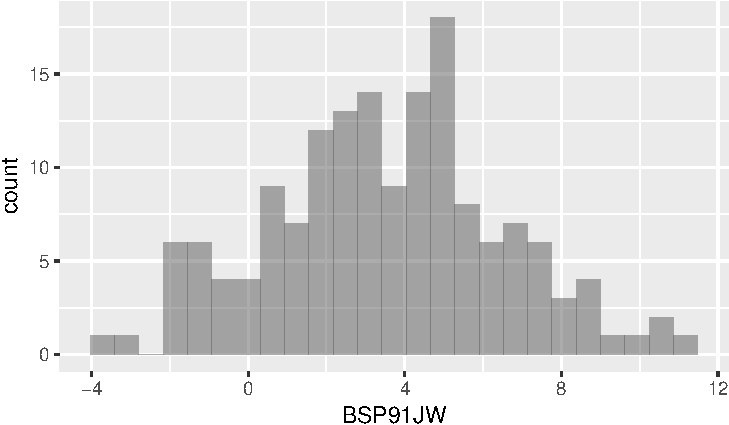
\includegraphics{DatenerhebungStatistik-Uebung_files/figure-latex/unnamed-chunk-123-1.pdf}

\begin{Shaded}
\begin{Highlighting}[]
\KeywordTok{favstats}\NormalTok{( }\OperatorTok{~}\StringTok{ }\NormalTok{BSP91JW, }\DataTypeTok{data =}\NormalTok{ B3)}
\end{Highlighting}
\end{Shaded}

\begin{verbatim}
##    min   Q1 median   Q3   max     mean       sd   n missing
##  -3.78 1.58   3.59 5.17 11.12 3.498662 2.974273 157       0
\end{verbatim}

Liefern die Daten Belege für die Forschungsthese, dass der Mittelwert
nicht zufällig \(> 0\,\%\) ist?

Zunächst ein Konfidenzintervall für den unbekannten Wert \(\mu\):

\begin{Shaded}
\begin{Highlighting}[]
\NormalTok{BootBSP91JW <-}\StringTok{ }\KeywordTok{do}\NormalTok{(}\DecValTok{10000}\NormalTok{) }\OperatorTok{*}\StringTok{ }\KeywordTok{mean}\NormalTok{( }\OperatorTok{~}\StringTok{ }\NormalTok{BSP91JW, }\DataTypeTok{data =} \KeywordTok{resample}\NormalTok{(B3))}
\KeywordTok{gf_histogram}\NormalTok{( }\OperatorTok{~}\StringTok{ }\NormalTok{mean, }\DataTypeTok{data =}\NormalTok{ BootBSP91JW)}
\end{Highlighting}
\end{Shaded}

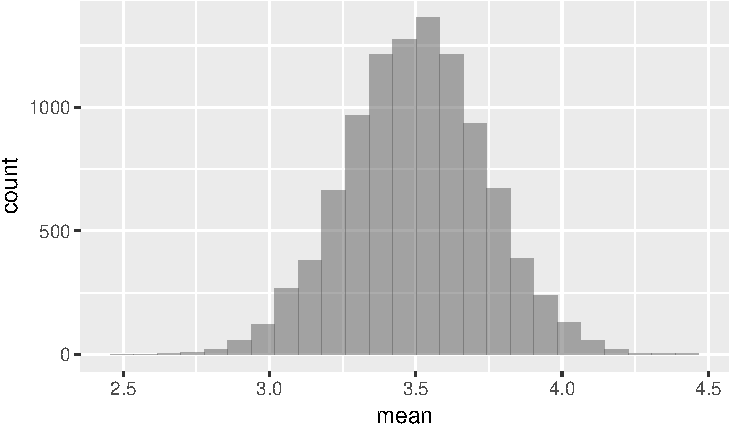
\includegraphics{DatenerhebungStatistik-Uebung_files/figure-latex/unnamed-chunk-124-1.pdf}

\begin{Shaded}
\begin{Highlighting}[]
\KeywordTok{quantile}\NormalTok{( }\OperatorTok{~}\StringTok{ }\NormalTok{mean, }\DataTypeTok{data =}\NormalTok{ BootBSP91JW, }\DataTypeTok{probs =} \KeywordTok{c}\NormalTok{(}\FloatTok{0.025}\NormalTok{, }\FloatTok{0.975}\NormalTok{))}
\end{Highlighting}
\end{Shaded}

\begin{verbatim}
##     2.5%    97.5% 
## 3.031462 3.968282
\end{verbatim}

Hier ist die \(0\) schon einmal nicht enthalten.

Unter der Annahme einer Normalverteilung kann (mit) der geschätzten
Standardabweichung eine Stichprobe der gegebenen Länge unter
\(H_0: \mu=0\) erzeugt werden:

\begin{Shaded}
\begin{Highlighting}[]
\CommentTok{# Mittelwert}
\NormalTok{meandBSP <-}\StringTok{ }\KeywordTok{mean}\NormalTok{( }\OperatorTok{~}\StringTok{ }\NormalTok{BSP91JW, }\DataTypeTok{data =}\NormalTok{ B3)}
\CommentTok{# Standardabweichung}
\NormalTok{sdBSP <-}\StringTok{ }\KeywordTok{sd}\NormalTok{( }\OperatorTok{~}\StringTok{ }\NormalTok{BSP91JW, }\DataTypeTok{data =}\NormalTok{ B3)}
\CommentTok{# Anzahl Beobachtungen}
\NormalTok{n <-}\StringTok{  }\KeywordTok{length}\NormalTok{( B3}\OperatorTok{$}\NormalTok{BSP91JW)}
\CommentTok{# Zufallszahlengenerator setzen}
\KeywordTok{set.seed}\NormalTok{(}\DecValTok{1896}\NormalTok{)}

\NormalTok{simBSP <-}\StringTok{ }\KeywordTok{rnorm}\NormalTok{(}\DataTypeTok{n =}\NormalTok{ n, }\DataTypeTok{mean =} \DecValTok{0}\NormalTok{, }\DataTypeTok{sd =}\NormalTok{ sdBSP)}
\KeywordTok{gf_histogram}\NormalTok{( }\OperatorTok{~}\StringTok{ }\NormalTok{simBSP)}
\end{Highlighting}
\end{Shaded}

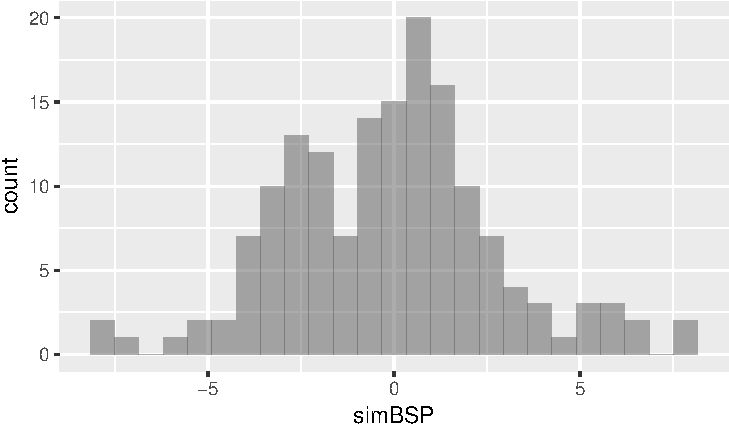
\includegraphics{DatenerhebungStatistik-Uebung_files/figure-latex/unnamed-chunk-125-1.pdf}

Für die Simulation der Verteilung unter \(H_0\) wird dies jetzt z.B.
\(10000\)-mal wiederholt -- und der Mittelwert berechnet:

\begin{Shaded}
\begin{Highlighting}[]
\NormalTok{SimBSP91JW <-}\StringTok{ }\KeywordTok{do}\NormalTok{(}\DecValTok{10000}\NormalTok{) }\OperatorTok{*}\StringTok{ }\KeywordTok{mean}\NormalTok{( }\OperatorTok{~}\StringTok{ }\KeywordTok{rnorm}\NormalTok{(}\DataTypeTok{n =}\NormalTok{ n, }\DataTypeTok{mean =} \DecValTok{0}\NormalTok{, }\DataTypeTok{sd =}\NormalTok{ sdBSP))}
\KeywordTok{gf_histogram}\NormalTok{( }\OperatorTok{~}\StringTok{ }\NormalTok{mean, }\DataTypeTok{data=}\NormalTok{SimBSP91JW)}
\end{Highlighting}
\end{Shaded}

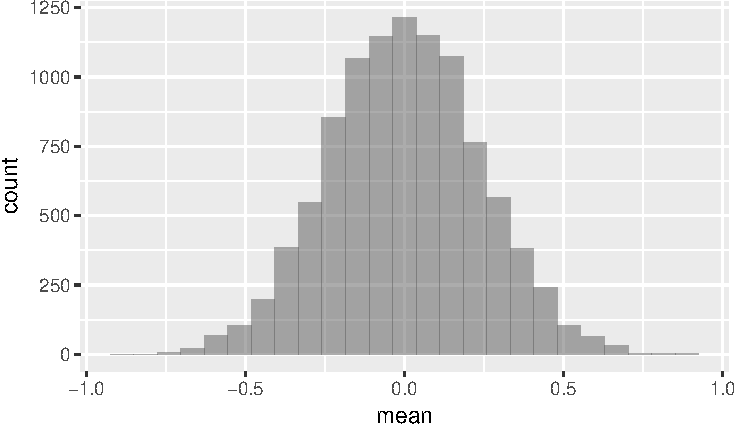
\includegraphics{DatenerhebungStatistik-Uebung_files/figure-latex/unnamed-chunk-126-1.pdf}

Der Anteil der unter \(H_0\) simulierten Daten, die einen größeren
Mittelwert als den beobachteten aufweisen ist sehr klein:

\begin{Shaded}
\begin{Highlighting}[]
\KeywordTok{prop}\NormalTok{( }\KeywordTok{mean}\NormalTok{( }\OperatorTok{~}\NormalTok{mean, }\DataTypeTok{data =}\NormalTok{ SimBSP91JW)}\OperatorTok{>=}\StringTok{ }\NormalTok{meandBSP)}
\end{Highlighting}
\end{Shaded}

\begin{verbatim}
## prop_TRUE 
##         0
\end{verbatim}

Der beobachtete Wert der Teststatistik ist also unter
\(H_0: \mu \leq 0\) sehr unwahrscheinlich, \(H_0\) würde also verworfen.

Dieses Ergebnis liefert auch der t-Test:

\begin{Shaded}
\begin{Highlighting}[]
\KeywordTok{t.test}\NormalTok{( }\OperatorTok{~}\StringTok{ }\NormalTok{BSP91JW, }\DataTypeTok{data =}\NormalTok{ B3, }\DataTypeTok{alternative =} \StringTok{"greater"}\NormalTok{)}
\end{Highlighting}
\end{Shaded}

\begin{verbatim}
## 
##  One Sample t-test
## 
## data:  BSP91JW
## t = 14.739, df = 156, p-value < 2.2e-16
## alternative hypothesis: true mean is greater than 0
## 95 percent confidence interval:
##  3.105886      Inf
## sample estimates:
## mean of x 
##  3.498662
\end{verbatim}

Oder eine Berechnung \enquote{per Hand}:

\begin{Shaded}
\begin{Highlighting}[]
\CommentTok{# Standardfehler}
\NormalTok{se <-}\StringTok{ }\NormalTok{sdBSP}\OperatorTok{/}\KeywordTok{sqrt}\NormalTok{(n)}
\CommentTok{# p-Wert}
\KeywordTok{xpnorm}\NormalTok{( meandBSP, }\DataTypeTok{mean =} \DecValTok{0}\NormalTok{, }\DataTypeTok{sd =}\NormalTok{ se, }\DataTypeTok{lower.tail =} \OtherTok{FALSE}\NormalTok{)}
\end{Highlighting}
\end{Shaded}

\begin{verbatim}
## 
\end{verbatim}

\begin{verbatim}
## If X ~ N(0, 0.2374), then
\end{verbatim}

\begin{verbatim}
##  P(X <= 3.499) = P(Z <= 14.74) = 1
\end{verbatim}

\begin{verbatim}
##  P(X >  3.499) = P(Z >  14.74) = 0
\end{verbatim}

\begin{verbatim}
## 
\end{verbatim}

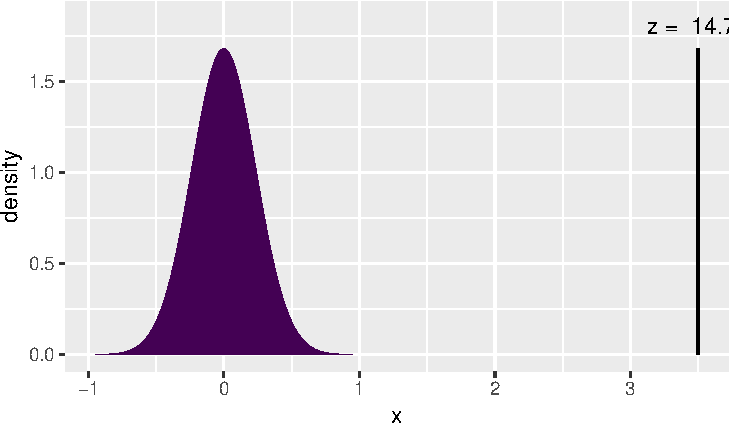
\includegraphics{DatenerhebungStatistik-Uebung_files/figure-latex/unnamed-chunk-129-1.pdf}

\begin{verbatim}
## [1] 1.807738e-49
\end{verbatim}

\hypertarget{t-test-fur-eine-abhangigegepaarte-stichprobe}{%
\section{t-Test für eine abhängige/gepaarte
Stichprobe}\label{t-test-fur-eine-abhangigegepaarte-stichprobe}}

Hier interessieren besonders die (Veränderung der) Investitionen in
Ausrüstungsgüter (\texttt{IAUJW91}) und in Bauten (\texttt{IB91JW}). Die
deskriptiven Kennzahlen zeigen,

\begin{Shaded}
\begin{Highlighting}[]
\KeywordTok{favstats}\NormalTok{( }\OperatorTok{~}\StringTok{ }\NormalTok{IAU91JW, }\DataTypeTok{data =}\NormalTok{ B3)}
\end{Highlighting}
\end{Shaded}

\begin{verbatim}
##     min    Q1 median  Q3   max     mean       sd   n missing
##  -19.95 -1.25    5.3 9.1 27.25 3.992675 8.864805 157       0
\end{verbatim}

\begin{Shaded}
\begin{Highlighting}[]
\KeywordTok{favstats}\NormalTok{( }\OperatorTok{~}\StringTok{ }\NormalTok{IB91JW, }\DataTypeTok{data =}\NormalTok{ B3)}
\end{Highlighting}
\end{Shaded}

\begin{verbatim}
##     min    Q1 median   Q3   max     mean       sd   n missing
##  -21.59 -1.16    2.6 5.55 40.25 2.565096 7.481063 157       0
\end{verbatim}

dass im betrachteten Zeitraum die Investitionen in Ausrüstungsgüter mit
dem arithmetischen Mittelwert von 3.99 im Mittel stärker gestiegen sind
als die in Bauten mit 2.57. Da die Investitionen sicherlich in
Zusammenhang mit der gesamten konjunkturellen Entwicklung stehen, ist
davon auszugehen, dass es sich hier um vom jeweiligen Zeitpunkt
abhängige Beobachtungen handelt. Daher wird hier die Differenz der Werte
betrachtet: \texttt{IB91JW\ -\ IAU91JW}. Der R Befehl für einen t-Test
lautet \texttt{t.test}:

\begin{Shaded}
\begin{Highlighting}[]
\KeywordTok{t.test}\NormalTok{ (}\OperatorTok{~}\StringTok{ }\NormalTok{(IB91JW }\OperatorTok{-}\StringTok{ }\NormalTok{IAU91JW), }\DataTypeTok{data =}\NormalTok{ B3)}
\end{Highlighting}
\end{Shaded}

\begin{verbatim}
## 
##  One Sample t-test
## 
## data:  IB91JW
## t = -1.9612, df = 156, p-value = 0.05164
## alternative hypothesis: true mean is not equal to 0
## 95 percent confidence interval:
##  -2.86544149  0.01028226
## sample estimates:
## mean of x 
##  -1.42758
\end{verbatim}

Der (umfangreichen) Ausgabe können Sie neben dem z- bzw. t-Wert (-1.96)
mit unter der Nullhypothese der Gleichheit des Lageparameters
\[H_0: \mu_{\text{IB91JW}-\text{IAU91JW}}=0\] insbesondere den p-Wert
(0.0516) und das Konfidenzintervall \((-2.87, 0.01)\) entnehmen. Zum
Signifikanznvieau von 5\(\,\)\% wird die Nullhypothese also gerade so
\emph{nicht} abgelehnt, da der p-Wert über 5\(\,\)\% liegt sowie der
Wert der Nullhypothese, \(\mu=0\), im Konfidenzintervall ist.

\begin{center}\rule{0.5\linewidth}{\linethickness}\end{center}

\textbf{Übung:}

\begin{enumerate}
\def\labelenumi{\arabic{enumi}.}
\tightlist
\item
  Testen Sie, ob es einen nicht zufälligen mittleren Lageunterschied
  zwischen der Veränderung des Preisindex des Bruttosozialproduktes
  \texttt{PBSPJW} und dem des privaten Verbrauchs \texttt{PCPJW} gibt.
\end{enumerate}

\begin{center}\rule{0.5\linewidth}{\linethickness}\end{center}

\hypertarget{t-test-fur-zwei-unabhangige-stichproben}{%
\section{t-Test für zwei unabhängige
Stichproben}\label{t-test-fur-zwei-unabhangige-stichproben}}

Untersuchen wir, ob sich makroökonomische Kennzahlen im Auf- und
Abschwung unterscheiden. Zunächst stellen wir fest, dass die eigentlich
kategorielle Variable \texttt{PHASEN} hier numerisch kodiert wurde, was
aber schnell verwirren würde.

\begin{Shaded}
\begin{Highlighting}[]
\KeywordTok{typeof}\NormalTok{(B3}\OperatorTok{$}\NormalTok{PHASEN)}
\end{Highlighting}
\end{Shaded}

\begin{verbatim}
## [1] "integer"
\end{verbatim}

Typänderung zu \texttt{factor} geht einfach:

\begin{Shaded}
\begin{Highlighting}[]
\NormalTok{B3}\OperatorTok{$}\NormalTok{PHASEN <-}\StringTok{ }\KeywordTok{as.factor}\NormalTok{(B3}\OperatorTok{$}\NormalTok{PHASEN)}
\end{Highlighting}
\end{Shaded}

Wenn wir die einzelnen \texttt{levels} des Faktors als numerische Werte
verwenden wollen, würden wir den Befehl \texttt{as.numeric()} verwenden.
Aber sicherheitshalber vorher über \texttt{levels()} schauen, ob die
Reihenfolge auch stimmt.

Um die Interpretation zu erleichtern können wir hier einfach die
Faktorstufe umbenennen.

\begin{Shaded}
\begin{Highlighting}[]
\KeywordTok{levels}\NormalTok{(B3}\OperatorTok{$}\NormalTok{PHASEN) <-}\StringTok{ }\KeywordTok{c}\NormalTok{(}\StringTok{"Aufschwung"}\NormalTok{, }\StringTok{"Oberer Wendepunkt"}\NormalTok{, }
                       \StringTok{"Abschwung"}\NormalTok{, }\StringTok{"Unterer Wendepunkt"}\NormalTok{)}
\end{Highlighting}
\end{Shaded}

Jetzt ist keine Verwechselung von kategoriellen und metrischen Variablen
mehr möglich.

Zunächst wird der Datensatz, der auch die konjunkturellen Wendepunkte
enthält, nur auf Auf- und Abschwung eingeschränkt.

\begin{Shaded}
\begin{Highlighting}[]
\NormalTok{B3AufAb <-}\StringTok{ }\KeywordTok{filter}\NormalTok{(B3, PHASEN }\OperatorTok\StringTok{ }\KeywordTok{c}\NormalTok{(}\StringTok{"Aufschwung"}\NormalTok{, }\StringTok{"Abschwung"}\NormalTok{)) }
\NormalTok{B3AufAb <-}\StringTok{ }\KeywordTok{droplevels}\NormalTok{(B3AufAb)}
\end{Highlighting}
\end{Shaded}

In der politischen Diskussion werden immer niedrige Zinsen gefordert.
Schauen wir mal, wie die Zinsen in den Konjunkturphasen in der
Vergangenheit (1955-1994) verteilt waren:

\begin{Shaded}
\begin{Highlighting}[]
\KeywordTok{gf_boxplot}\NormalTok{(ZINSK }\OperatorTok{~}\StringTok{ }\NormalTok{PHASEN, }\DataTypeTok{data =}\NormalTok{ B3AufAb)}
\end{Highlighting}
\end{Shaded}

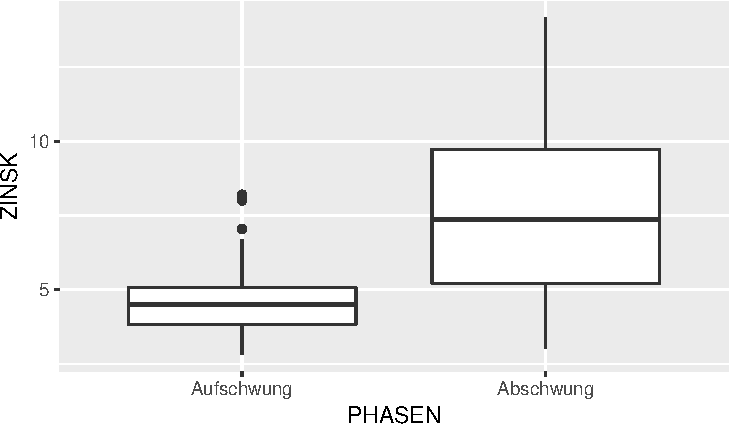
\includegraphics{DatenerhebungStatistik-Uebung_files/figure-latex/unnamed-chunk-137-1.pdf}

Anscheinend waren die Zinsen in Zeiten des Aufschwungs niedriger.

Was sagen die deskriptiven Kennzahlen?

\begin{Shaded}
\begin{Highlighting}[]
\KeywordTok{favstats}\NormalTok{(ZINSK }\OperatorTok{~}\StringTok{ }\NormalTok{PHASEN, }\DataTypeTok{data =}\NormalTok{ B3AufAb)}
\end{Highlighting}
\end{Shaded}

\begin{verbatim}
##       PHASEN  min    Q1 median    Q3   max     mean       sd  n missing
## 1 Aufschwung 2.81 3.830   4.50 5.065  8.20 4.715085 1.209989 59       0
## 2  Abschwung 3.00 5.205   7.37 9.735 14.17 7.682553 3.020254 47       0
\end{verbatim}

Alle Lagemaße für die Zinskosten sind in der Aufschwungphase niedriger.

Der t-Test der Zinskosten für
\[H_0: \mu_{\text{Aufschwung}}=\mu_{\text{Abschwung}} \Leftrightarrow \mu_{\text{Aufschwung}}-\mu_{\text{Abschwung}}=0\]
mit der Teststatistik
\[T=\frac{\bar{x}_A-\bar{x}_B}{\sqrt{\frac{sd^2_A}{{n_A}}+\frac{sd^2_B}{{n_B}}}}\]
hat dann den gleichen Aufbau der Syntax wie \texttt{bwplot} oder
\texttt{favstats}: Teste die Zinskosten in Abhängigkeit der
Konjunkturphase.

Die Berechnung der Teststatistik

\begin{Shaded}
\begin{Highlighting}[]
\KeywordTok{t.test}\NormalTok{(ZINSK }\OperatorTok{~}\StringTok{ }\NormalTok{PHASEN, }\DataTypeTok{data =}\NormalTok{ B3AufAb)}
\end{Highlighting}
\end{Shaded}

\begin{verbatim}
## 
##  Welch Two Sample t-test
## 
## data:  ZINSK by PHASEN
## t = -6.3426, df = 57.766, p-value = 3.743e-08
## alternative hypothesis: true difference in means is not equal to 0
## 95 percent confidence interval:
##  -3.904085 -2.030852
## sample estimates:
## mean in group Aufschwung  mean in group Abschwung 
##                 4.715085                 7.682553
\end{verbatim}

Der kleine p-Wert von \(3.7430775\times 10^{-8}\) zeigt, dass die
Nullhypothese der Gleichheit der Lageparameter verworfen werden kann.
Wir können der Funktion auch eine spezielle Alternativhypothese
übergeben:

\begin{Shaded}
\begin{Highlighting}[]
\KeywordTok{t.test}\NormalTok{(ZINSK }\OperatorTok{~}\StringTok{ }\NormalTok{PHASEN, }\DataTypeTok{data =}\NormalTok{ B3AufAb, }\DataTypeTok{alternative =} \StringTok{"less"}\NormalTok{)}
\end{Highlighting}
\end{Shaded}

\begin{verbatim}
## 
##  Welch Two Sample t-test
## 
## data:  ZINSK by PHASEN
## t = -6.3426, df = 57.766, p-value = 1.872e-08
## alternative hypothesis: true difference in means is less than 0
## 95 percent confidence interval:
##       -Inf -2.185354
## sample estimates:
## mean in group Aufschwung  mean in group Abschwung 
##                 4.715085                 7.682553
\end{verbatim}

Jetzt haben wir die Nullhypothese \enquote{Das Lagemaß für die
Zinskosten ist im Aufschwung \emph{nicht} kleiner als im Abschwung}
gegen die Alternativhypothese (Forschungshypothese) \enquote{Das Lagemaß
für die Zinskosten ist im Aufschwung kleiner als im Abschwung} getestet:
\[H_0: \mu_{\text{Aufschwung}} \geq \mu_{\text{Abschwung}} \quad vs. \quad H_A: \mu_{\text{Aufschwung}} < \mu_{\text{Abschwung}}\]
bzw.
\[H_0: \mu_{\text{Aufschwung}} - \mu_{\text{Abschwung}} \geq 0 \quad vs. \quad H_A: \mu_{\text{Aufschwung}} - \mu_{\text{Abschwung}} < 0 \]

\begin{center}\rule{0.5\linewidth}{\linethickness}\end{center}

\textbf{Übung:}

\begin{enumerate}
\def\labelenumi{\arabic{enumi}.}
\setcounter{enumi}{1}
\tightlist
\item
  Untersuchen Sie, ob sich die mittlere Entwicklung des privaten
  Verbrauchs \texttt{CP91JW} zwischen den Konjunkturphasen
  unterscheidet.
\end{enumerate}

\begin{center}\rule{0.5\linewidth}{\linethickness}\end{center}

Auch hier können wir, ohne eine Verteilungsannahme zu verwenden,
permutieren.

\begin{Shaded}
\begin{Highlighting}[]
\NormalTok{mdiff <-}\StringTok{ }\KeywordTok{diffmean}\NormalTok{(ZINSK }\OperatorTok{~}\StringTok{ }\NormalTok{PHASEN, }\DataTypeTok{data =}\NormalTok{ B3AufAb)}
\NormalTok{mdiff}
\end{Highlighting}
\end{Shaded}

\begin{verbatim}
## diffmean 
## 2.967468
\end{verbatim}

\begin{Shaded}
\begin{Highlighting}[]
\NormalTok{mdiff.null <-}\StringTok{ }\KeywordTok{do}\NormalTok{(}\DecValTok{10000}\NormalTok{) }\OperatorTok{*}\StringTok{ }\KeywordTok{diffmean}\NormalTok{(ZINSK }\OperatorTok{~}\StringTok{ }\KeywordTok{shuffle}\NormalTok{(PHASEN), }\DataTypeTok{data =}\NormalTok{ B3AufAb)}
\end{Highlighting}
\end{Shaded}

Unter der Nullhypothese der Gleichheit der Lagemaße kommt eine gleich
große oder größere Differenz also

\begin{Shaded}
\begin{Highlighting}[]
\KeywordTok{prop}\NormalTok{(}\OperatorTok{~}\NormalTok{diffmean }\OperatorTok{>=}\StringTok{ }\NormalTok{mdiff, }\DataTypeTok{data =}\NormalTok{ mdiff.null)}
\end{Highlighting}
\end{Shaded}

\begin{verbatim}
## prop_TRUE 
##         0
\end{verbatim}

mal vor!

Da die statistische \emph{Signifikanz} vom Standardfehler abhängt,
welcher wiederum vom Stichprobenumfang abhängt, wurde von Cohen ein Maß
für die \emph{Effektstärke}, \textbf{Cohen's d} vorgeschlagen:
\[d=\frac{\bar{x}_A-\bar{x}_B}{sd_{\text{pool}}}\] mit
\[{sd_{\text{pool}}=\sqrt{\frac{1}{n_A+n_B-2}\Bigl((n_A-1)sd^2_A+(n_B-1)sd^2_B \Bigr)}}\]

\begin{Shaded}
\begin{Highlighting}[]
\CommentTok{# Kennzahlen 1. Stichprobe}
\NormalTok{m1 <-}\StringTok{ }\KeywordTok{mean}\NormalTok{(B3}\OperatorTok{$}\NormalTok{ZINSK[B3}\OperatorTok{$}\NormalTok{PHASEN }\OperatorTok{==}\StringTok{ "Aufschwung"}\NormalTok{]) }
\NormalTok{sd1 <-}\StringTok{ }\KeywordTok{sd}\NormalTok{(B3}\OperatorTok{$}\NormalTok{ZINSK[B3}\OperatorTok{$}\NormalTok{PHASEN }\OperatorTok{==}\StringTok{ "Aufschwung"}\NormalTok{]) }
\NormalTok{n1 <-}\StringTok{ }\KeywordTok{length}\NormalTok{(B3}\OperatorTok{$}\NormalTok{ZINSK[B3}\OperatorTok{$}\NormalTok{PHASEN }\OperatorTok{==}\StringTok{ "Aufschwung"}\NormalTok{])}
\CommentTok{# Kennzahlen 2. Stichprobe}
\NormalTok{m2 <-}\StringTok{ }\KeywordTok{mean}\NormalTok{(B3}\OperatorTok{$}\NormalTok{ZINSK[B3}\OperatorTok{$}\NormalTok{PHASEN }\OperatorTok{==}\StringTok{ "Abschwung"}\NormalTok{]) }
\NormalTok{sd2 <-}\StringTok{ }\KeywordTok{sd}\NormalTok{(B3}\OperatorTok{$}\NormalTok{ZINSK[B3}\OperatorTok{$}\NormalTok{PHASEN }\OperatorTok{==}\StringTok{ "Abschwung"}\NormalTok{]) }
\NormalTok{n2 <-}\StringTok{ }\KeywordTok{length}\NormalTok{(B3}\OperatorTok{$}\NormalTok{ZINSK[B3}\OperatorTok{$}\NormalTok{PHASEN }\OperatorTok{==}\StringTok{ "Abschwung"}\NormalTok{])}
\CommentTok{# Gepoolte Standardabweichung}
\NormalTok{sdpool <-}\StringTok{ }\KeywordTok{sqrt}\NormalTok{( ((n1}\DecValTok{-1}\NormalTok{)}\OperatorTok{*}\NormalTok{sd1}\OperatorTok{^}\DecValTok{2} \OperatorTok{+}\StringTok{ }\NormalTok{(n2}\DecValTok{-1}\NormalTok{)}\OperatorTok{*}\NormalTok{sd2}\OperatorTok{^}\DecValTok{2}\NormalTok{) }\OperatorTok{/}\StringTok{ }\NormalTok{(n1}\OperatorTok{+}\NormalTok{n2}\DecValTok{-2}\NormalTok{))}
\CommentTok{# Cohen's d}
\NormalTok{d <-}\StringTok{ }\NormalTok{(m1}\OperatorTok{-}\NormalTok{m2)}\OperatorTok{/}\NormalTok{sdpool}
\NormalTok{d}
\end{Highlighting}
\end{Shaded}

\begin{verbatim}
## [1] -1.347291
\end{verbatim}

Cohen's d ist ein Maß der Überlappung der Verteilungen:

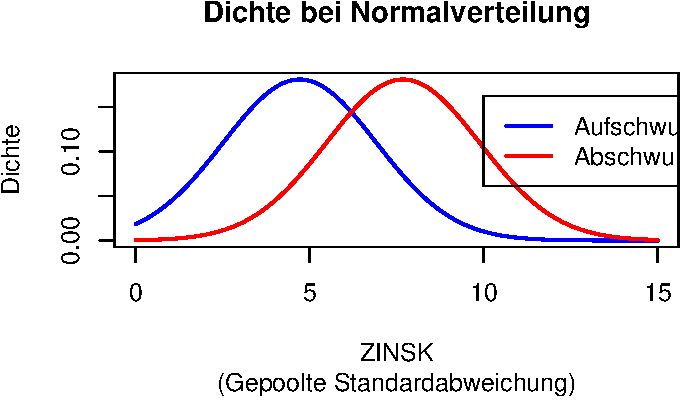
\includegraphics{DatenerhebungStatistik-Uebung_files/figure-latex/unnamed-chunk-145-1.pdf}

Häufig werden Werte

\begin{itemize}
\tightlist
\item
  \(|d|\leq 0.2\) als kleine
\item
  \(|d|\leq 0.5\) als mittlere
\item
  \(|d|\geq 0.8\) als große Effekte
\end{itemize}

bezeichnet.

Eine direkte Berechnung geht über das Paket \texttt{lsr}:

\begin{Shaded}
\begin{Highlighting}[]
\CommentTok{# Einmalig installieren:}
\CommentTok{# install.packages("lsr")}
\KeywordTok{library}\NormalTok{(lsr)}
\KeywordTok{cohensD}\NormalTok{(ZINSK }\OperatorTok{~}\StringTok{ }\NormalTok{PHASEN, }\DataTypeTok{data =}\NormalTok{ B3AufAb)}
\end{Highlighting}
\end{Shaded}

\begin{verbatim}
## [1] 1.347291
\end{verbatim}

\hypertarget{varianzanalyse-anova}{%
\section{Varianzanalyse (ANOVA)}\label{varianzanalyse-anova}}

Bei mehr als zwei Gruppen funktionieren die Techniken des t-Tests nicht
mehr. Um Lagemaßunterschiede zu testen, wird anstelle der Mittelwerte
die Streuung verglichen: Ist die Streuung zwischen den Gruppen groß im
Vergleich zur Streuung innerhalb der Gruppen?

\begin{Shaded}
\begin{Highlighting}[]
\KeywordTok{gf_point}\NormalTok{(DEFRATE }\OperatorTok{~}\StringTok{ }\NormalTok{PHASEN, }\DataTypeTok{data =}\NormalTok{ B3)}
\end{Highlighting}
\end{Shaded}

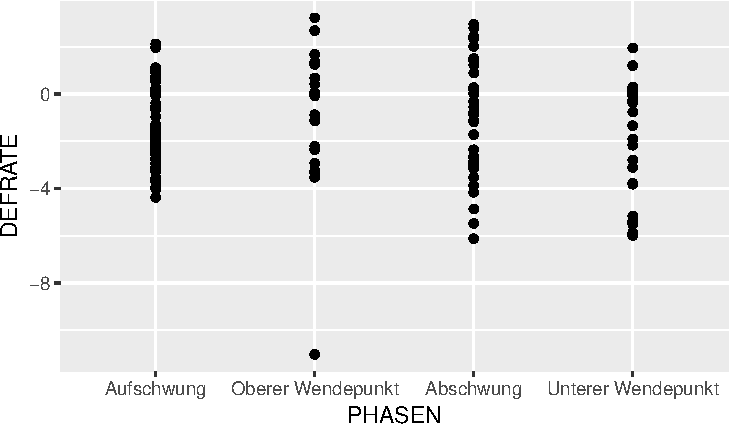
\includegraphics{DatenerhebungStatistik-Uebung_files/figure-latex/unnamed-chunk-147-1.pdf}

Es gilt, dass sich die Gesamtstreung (\(SST\)) zusammensetzt aus der
Streuung zwischen den Gruppen (\(SSG\)) und innerhalb der Gruppen
(\(SSE\)), d.~h., \[SST=SSG+SSE.\]

Unterscheidet sich der mittlere Anteil des Staatsdefizits
\texttt{DEFRATE} nicht zufällig zwischen den Konjunkturphasen?

\begin{Shaded}
\begin{Highlighting}[]
\KeywordTok{gf_boxplot}\NormalTok{(DEFRATE }\OperatorTok{~}\StringTok{ }\NormalTok{PHASEN, }\DataTypeTok{data =}\NormalTok{ B3)}
\end{Highlighting}
\end{Shaded}

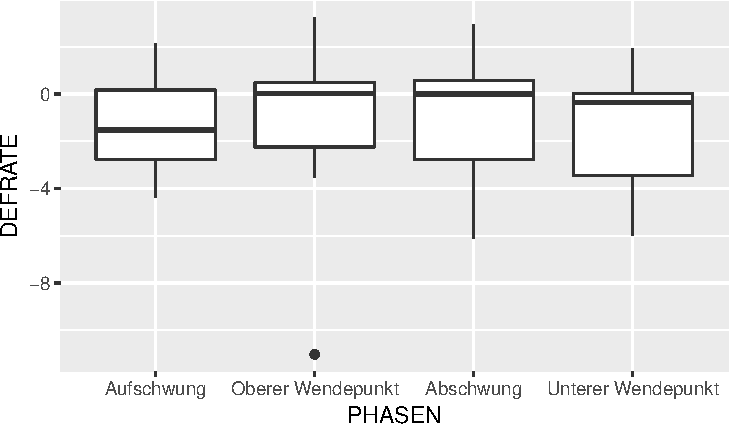
\includegraphics{DatenerhebungStatistik-Uebung_files/figure-latex/unnamed-chunk-148-1.pdf}

\begin{Shaded}
\begin{Highlighting}[]
\KeywordTok{favstats}\NormalTok{(DEFRATE }\OperatorTok{~}\StringTok{ }\NormalTok{PHASEN, }\DataTypeTok{data =}\NormalTok{ B3)}
\end{Highlighting}
\end{Shaded}

\begin{verbatim}
##               PHASEN    min      Q1 median     Q3  max       mean       sd
## 1         Aufschwung  -4.38 -2.7650  -1.52 0.1650 2.12 -1.3394915 1.680638
## 2  Oberer Wendepunkt -11.02 -2.2475   0.02 0.4775 3.22 -0.8479167 2.836558
## 3          Abschwung  -6.12 -2.7850   0.00 0.5800 2.95 -0.8380851 2.287536
## 4 Unterer Wendepunkt  -5.99 -3.4450  -0.37 0.0250 1.94 -1.6548148 2.364026
##    n missing
## 1 59       0
## 2 24       0
## 3 47       0
## 4 27       0
\end{verbatim}

Vielleicht, vielleicht nicht.

Um eine Varianzanalyse (\emph{Analysis of Variance, ANOVA}) mit
\[H_0: \mu_1=\mu_2=\ldots =\mu_k\] gegen
\[H_A: \text{Mindestens ein } \mu_i \text{ ist verschieden.}\]
durchzuführen kann in R u. a. der Befehl \texttt{aov} verwendet werden:

\begin{Shaded}
\begin{Highlighting}[]
\NormalTok{DEFaov <-}\StringTok{ }\KeywordTok{aov}\NormalTok{(DEFRATE }\OperatorTok{~}\StringTok{ }\NormalTok{PHASEN, }\DataTypeTok{data =}\NormalTok{ B3)}
\KeywordTok{summary}\NormalTok{(DEFaov)}
\end{Highlighting}
\end{Shaded}

\begin{verbatim}
##              Df Sum Sq Mean Sq F value Pr(>F)
## PHASEN        3   15.7   5.236    1.09  0.355
## Residuals   153  734.9   4.803
\end{verbatim}

Der p-Wert des F-Tests der Nullhypothese
\[H_0: \mu_{\text{Aufschwung}}=\mu_{\text{Oberer Wendepunt}}=\mu_{\text{Abschwung}}=\mu_{\text{Unterer Wendepunkt}}\]
der Gleichheit der Lage ist mit 0.3552 größer als 0.05, die
Nullhypothese kann also für das Staatsdefizit nicht verworfen werden.

Bei \(k\) Gruppen ist die mittlere quadratische Varianz
\(MSG=\frac{1}{k-1}\sum_{i=1}^k n_i (\bar{x}_i- \bar{x})^2=\frac{SSG}{\underbrace{k-1}_{df_G}}\)
(\(n_i\) ist die Anzahl Beobachtungen in Gruppe \(i\), \(\bar{x}_i\) der
Gruppenmittelwert und \(\bar{x}\) der Gesamtmittelwert.) Hier also
\(MSG=5.2361\). Der mittlere quadratische Fehler, \(MSE\), ist dann
\(MSE=\frac{1}{n-k} \sum_{i=1}^k (n_i-1) sd^2_i=\frac{SSE}{\underbrace{n-k}_{df_E}}\),
mit \(sd_i\) der Standardabweichung in Gruppe \(i\). Hier:
\(MSE=4.8032\).

Der Wert der Teststatistik \(F\) ist dann
\[F=\frac{MSG}{MSE}=\frac{5.2361}{4.8032}=1.0901.\]

Unterscheidet sich das Lagemaß der Veränderung der Lohnstückkosten
\texttt{LSTKJW} nicht zufällig?

\begin{Shaded}
\begin{Highlighting}[]
\KeywordTok{gf_boxplot}\NormalTok{(LSTKJW }\OperatorTok{~}\StringTok{ }\NormalTok{PHASEN, }\DataTypeTok{data =}\NormalTok{ B3)}
\end{Highlighting}
\end{Shaded}

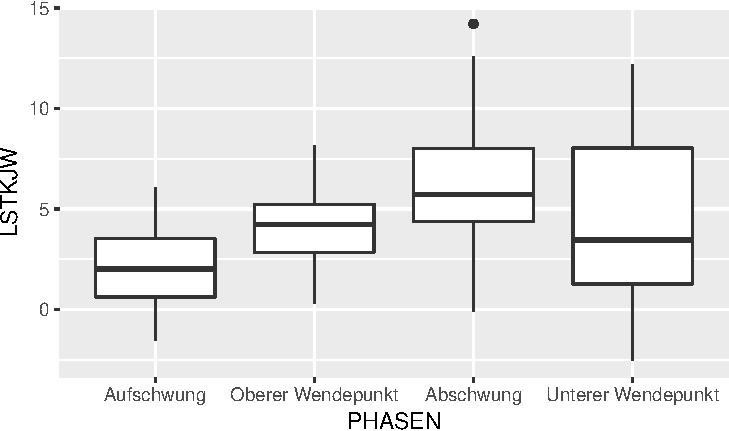
\includegraphics{DatenerhebungStatistik-Uebung_files/figure-latex/unnamed-chunk-150-1.pdf}

\begin{Shaded}
\begin{Highlighting}[]
\KeywordTok{favstats}\NormalTok{(LSTKJW }\OperatorTok{~}\StringTok{ }\NormalTok{PHASEN, }\DataTypeTok{data =}\NormalTok{ B3)}
\end{Highlighting}
\end{Shaded}

\begin{verbatim}
##               PHASEN   min    Q1 median     Q3   max     mean       sd  n
## 1         Aufschwung -1.54 0.625   2.02 3.5250  6.09 2.111017 1.837423 59
## 2  Oberer Wendepunkt  0.32 2.840   4.22 5.2225  8.16 4.195833 2.074516 24
## 3          Abschwung -0.12 4.385   5.71 8.0100 14.21 6.291064 3.122604 47
## 4 Unterer Wendepunkt -2.53 1.270   3.46 8.0350 12.18 4.249630 4.449861 27
##   missing
## 1       0
## 2       0
## 3       0
## 4       0
\end{verbatim}

\begin{Shaded}
\begin{Highlighting}[]
\NormalTok{LSTKaov <-}\StringTok{ }\KeywordTok{aov}\NormalTok{(LSTKJW }\OperatorTok{~}\StringTok{ }\NormalTok{PHASEN, }\DataTypeTok{data =}\NormalTok{ B3)}
\KeywordTok{summary}\NormalTok{(LSTKaov)}
\end{Highlighting}
\end{Shaded}

\begin{verbatim}
##              Df Sum Sq Mean Sq F value   Pr(>F)    
## PHASEN        3  459.5  153.15   18.62 2.37e-10 ***
## Residuals   153 1258.2    8.22                     
## ---
## Signif. codes:  0 '***' 0.001 '**' 0.01 '*' 0.05 '.' 0.1 ' ' 1
\end{verbatim}

Die Nullhypothese der Gleichheit wird hier also verworfen.
Interessanterweise unterscheiden sich insbesondere die Lagemaße von Auf-
und Abschwung, die beiden Wendepunkte liegen dazwischen.

Im Paket \texttt{effects} gibt es übrigens eine schöne Plotfunktion für
die Effekte:

\begin{Shaded}
\begin{Highlighting}[]
\CommentTok{# Einmalig installieren:}
\CommentTok{# install.packages("effects")}
\KeywordTok{library}\NormalTok{(effects)}
\end{Highlighting}
\end{Shaded}

\begin{verbatim}
## Loading required package: carData
\end{verbatim}

\begin{verbatim}
## Use the command
##     lattice::trellis.par.set(effectsTheme())
##   to customize lattice options for effects plots.
## See ?effectsTheme for details.
\end{verbatim}

\begin{Shaded}
\begin{Highlighting}[]
\KeywordTok{plot}\NormalTok{(}\KeywordTok{allEffects}\NormalTok{(LSTKaov))}
\end{Highlighting}
\end{Shaded}

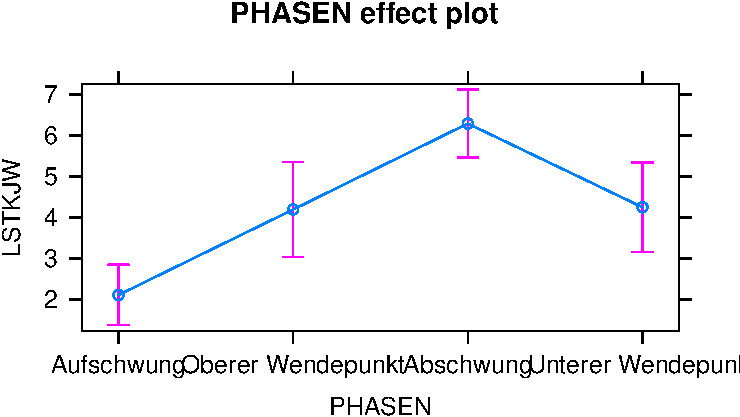
\includegraphics{DatenerhebungStatistik-Uebung_files/figure-latex/unnamed-chunk-151-1.pdf}

Neben dem arithmetischen Mittelwert (Punktschätzer) wird in der
Standardeinstellung das 95\(\,\)\% Konfidenzintervall eingezeichnet.

Um nach einer signifikanten Varianzanalyse sogenannte Post-Hoc Analysen
durchzuführen (z. B. welche der paarweisen Vergleiche sind signifikant?)
kann die Funktion \texttt{TukeyHSD()} (Tukey's \enquote{Honest
Significant Difference}) verwendet werden. Aufgrund des multiplen
Testproblems (Kumulierung Fehler 1. Art) müssen die p-Werte angepasst
werden.

\begin{Shaded}
\begin{Highlighting}[]
\NormalTok{LSTKposthoc <-}\StringTok{ }\KeywordTok{TukeyHSD}\NormalTok{(LSTKaov)}
\NormalTok{LSTKposthoc}
\end{Highlighting}
\end{Shaded}

\begin{verbatim}
##   Tukey multiple comparisons of means
##     95% family-wise confidence level
## 
## Fit: aov(formula = LSTKJW ~ PHASEN, data = B3)
## 
## $PHASEN
##                                            diff        lwr       upr
## Oberer Wendepunkt-Aufschwung          2.0848164  0.2814507  3.888182
## Abschwung-Aufschwung                  4.1800469  2.7237350  5.636359
## Unterer Wendepunkt-Aufschwung         2.1386127  0.4079289  3.869296
## Abschwung-Oberer Wendepunkt           2.0952305  0.2264813  3.963980
## Unterer Wendepunkt-Oberer Wendepunkt  0.0537963 -2.0358558  2.143448
## Unterer Wendepunkt-Abschwung         -2.0414342 -3.8401454 -0.242723
##                                          p adj
## Oberer Wendepunkt-Aufschwung         0.0163388
## Abschwung-Aufschwung                 0.0000000
## Unterer Wendepunkt-Aufschwung        0.0087085
## Abschwung-Oberer Wendepunkt          0.0212622
## Unterer Wendepunkt-Oberer Wendepunkt 0.9998923
## Unterer Wendepunkt-Abschwung         0.0191825
\end{verbatim}

\begin{Shaded}
\begin{Highlighting}[]
\KeywordTok{plot}\NormalTok{(LSTKposthoc)}
\end{Highlighting}
\end{Shaded}

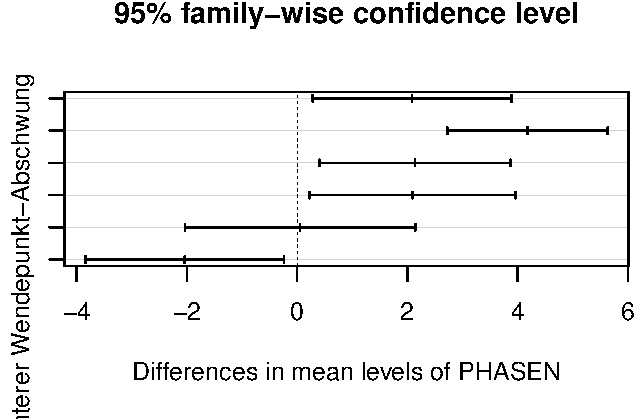
\includegraphics{DatenerhebungStatistik-Uebung_files/figure-latex/unnamed-chunk-152-1.pdf}

Hinweis: Da die einzelnen Faktorstufen hier unbalanciert sind (d .h.,
unterschiedliche Stichprobenumfänge haben) ist das Ergebnis hier nicht
exakt.

\begin{center}\rule{0.5\linewidth}{\linethickness}\end{center}

\textbf{Übung:}

\begin{enumerate}
\def\labelenumi{\arabic{enumi}.}
\setcounter{enumi}{2}
\tightlist
\item
  Gibt es nicht zufällige Lageunterschiede bei der Änderung der
  Erwerbstätigen \texttt{EWAJW} zwischen den Konjunkturphasen?
\end{enumerate}

\begin{center}\rule{0.5\linewidth}{\linethickness}\end{center}

\hypertarget{erweiterung-mehrfaktorielle-varianzanalyse-mit-wechselwirkung}{%
\subsection{Erweiterung: Mehrfaktorielle Varianzanalyse mit
Wechselwirkung}\label{erweiterung-mehrfaktorielle-varianzanalyse-mit-wechselwirkung}}

Betrachten wir noch einmal den \emph{tips} Datensatz aus \emph{Bryant,
P. G. and Smith, M (1995) Practical Data Analysis: Case Studies in
Business Statistics. Homewood, IL: Richard D. Irwin
Publishing}.\footnote{Anders als im Paper (und im Paket \texttt{AER})
  wird hier nur ein zufälliger Kurs je Dozent verwendet.}

Sofern noch nicht geschehen, können Sie in
\href{https://goo.gl/whKjnl}{hier} als \texttt{csv}-Datei herunterladen:

\begin{Shaded}
\begin{Highlighting}[]
\KeywordTok{download.file}\NormalTok{(}\StringTok{"https://goo.gl/whKjnl"}\NormalTok{, }\DataTypeTok{destfile =} \StringTok{"tips.csv"}\NormalTok{)}
\end{Highlighting}
\end{Shaded}

Das Einlesen der Daten in R erfolgt, sofern die Daten im
Arbeitsverzeichnis liegen, über:

\begin{Shaded}
\begin{Highlighting}[]
\NormalTok{tips <-}\StringTok{ }\KeywordTok{read.csv2}\NormalTok{(}\StringTok{"tips.csv"}\NormalTok{)}
\end{Highlighting}
\end{Shaded}

Um zu schauen, inwieweit das Trinkgeld vom Geschlecht \emph{und} dem
Rauchverhalten abhängt, kann folgende Analyse durchgeführt werden:

\begin{Shaded}
\begin{Highlighting}[]
\KeywordTok{favstats}\NormalTok{(tip }\OperatorTok{~}\StringTok{ }\NormalTok{sex }\OperatorTok{+}\StringTok{ }\NormalTok{smoker, }\DataTypeTok{data =}\NormalTok{ tips)}
\end{Highlighting}
\end{Shaded}

\begin{verbatim}
##   sex.smoker  min Q1 median     Q3  max     mean       sd  n missing
## 1  Female.No 1.00  2   2.68 3.4375  5.2 2.773519 1.128425 54       0
## 2    Male.No 1.25  2   2.74 3.7100  9.0 3.113402 1.489559 97       0
## 3 Female.Yes 1.00  2   2.88 3.5000  6.5 2.931515 1.219916 33       0
## 4   Male.Yes 1.00  2   3.00 3.8200 10.0 3.051167 1.500120 60       0
\end{verbatim}

\begin{Shaded}
\begin{Highlighting}[]
\NormalTok{tipaov <-}\StringTok{ }\KeywordTok{aov}\NormalTok{(tip }\OperatorTok{~}\StringTok{ }\NormalTok{sex }\OperatorTok{+}\StringTok{ }\NormalTok{smoker, }\DataTypeTok{data =}\NormalTok{ tips)}
\KeywordTok{summary}\NormalTok{(tipaov)}
\end{Highlighting}
\end{Shaded}

\begin{verbatim}
##              Df Sum Sq Mean Sq F value Pr(>F)
## sex           1    3.7   3.674   1.918  0.167
## smoker        1    0.0   0.015   0.008  0.930
## Residuals   241  461.5   1.915
\end{verbatim}

\begin{Shaded}
\begin{Highlighting}[]
\KeywordTok{plot}\NormalTok{(}\KeywordTok{allEffects}\NormalTok{(tipaov))}
\end{Highlighting}
\end{Shaded}

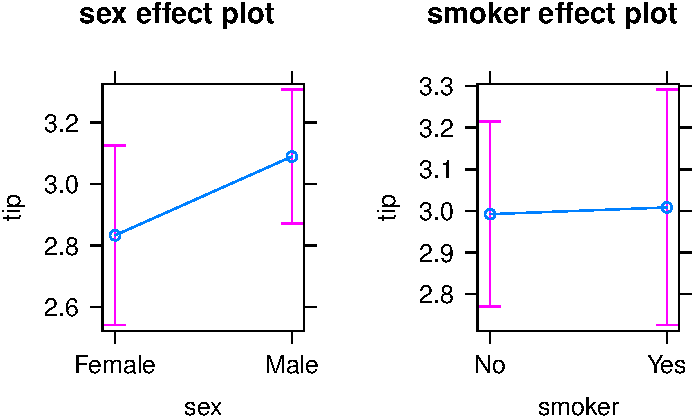
\includegraphics{DatenerhebungStatistik-Uebung_files/figure-latex/unnamed-chunk-155-1.pdf}

Beide Faktoren sind zum Signifikanzniveau 5\(\,\)\% \emph{nicht}
signifikant, d.~h., \(H_0\), dass sich die Mittelwerte in der Population
nicht unterscheiden, wird nicht verworfen.

Allerdings beobachten wir etwas anderes: Während der Mittelwert des
Trinkgeldes bei den Frauen bei den Rauchern größer ist, ist es bei den
Männern umgekehrt. Hier könnte also eine Wechselwirkung, eine
Interaktion, vorliegen. Diese wird in R über ein \texttt{:} in der
Formel eingefügt:

\begin{Shaded}
\begin{Highlighting}[]
\NormalTok{tipaovww <-}\StringTok{ }\KeywordTok{aov}\NormalTok{(tip }\OperatorTok{~}\StringTok{ }\NormalTok{sex }\OperatorTok{+}\StringTok{ }\NormalTok{smoker }\OperatorTok{+}\StringTok{ }\NormalTok{sex}\OperatorTok{:}\NormalTok{smoker, }\DataTypeTok{data =}\NormalTok{ tips)}
\KeywordTok{summary}\NormalTok{(tipaovww)}
\end{Highlighting}
\end{Shaded}

\begin{verbatim}
##              Df Sum Sq Mean Sq F value Pr(>F)
## sex           1    3.7   3.674   1.913  0.168
## smoker        1    0.0   0.015   0.008  0.930
## sex:smoker    1    0.6   0.640   0.333  0.564
## Residuals   240  460.9   1.920
\end{verbatim}

\begin{Shaded}
\begin{Highlighting}[]
\KeywordTok{plot}\NormalTok{(}\KeywordTok{allEffects}\NormalTok{(tipaovww ))}
\end{Highlighting}
\end{Shaded}

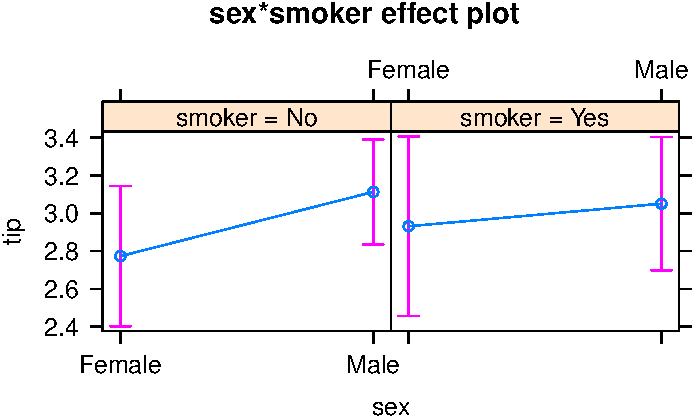
\includegraphics{DatenerhebungStatistik-Uebung_files/figure-latex/unnamed-chunk-156-1.pdf}

Auch hier gilt: Mit einem p-Wert von \(0.564\) wird die Nullhypothese,
dass in der Population keine Wechselwirkung von Geschlecht und
Rauchverhalten für den Mittelwert vorliegt, nicht verworfen.

\hypertarget{ubung-teaching-rating-2}{%
\section{Übung: Teaching Rating}\label{ubung-teaching-rating-2}}

Dieser Datensatz analysiert u. a. den Zusammenhang zwischen Schönheit
und Evaluierungsergebnis von Dozenten:

\emph{Hamermesh, D.S., and Parker, A. (2005). Beauty in the Classroom:
Instructors' Pulchritude and Putative Pedagogical Productivity.
Economics of Education Review, 24, 369--376.}

Sie können ihn, sofern noch nicht geschehen, von
\url{https://goo.gl/6Y3KoK} als \texttt{csv} herunterladen.

\begin{enumerate}
\def\labelenumi{\arabic{enumi}.}
\tightlist
\item
  Ist das arithmetische Mittel der Evaluierung \texttt{eval} nicht
  zufällig größer als befriedigend (3)?
\item
  Gibt es einen nicht zufälligen Unterschied im Lagemaß der Evaluation
  \texttt{eval} zwischen männlichen und weiblichen Dozent/innen
  (\texttt{gender})?
\end{enumerate}

\hypertarget{literatur-4}{%
\section{Literatur}\label{literatur-4}}

\begin{itemize}
\tightlist
\item
  David M. Diez, Christopher D. Barr, Mine Çetinkaya-Rundel (2014):
  \emph{Introductory Statistics with Randomization and Simulation},
  \url{https://www.openintro.org/stat/textbook.php?stat_book=isrs},
  Kapitel 4
\item
  Nicholas J. Horton, Randall Pruim, Daniel T. Kaplan (2015): Project
  MOSAIC Little Books \emph{A Student's Guide to R},
  \url{https://github.com/ProjectMOSAIC/LittleBooks/raw/master/StudentGuide/MOSAIC-StudentGuide.pdf},
  Kapitel 7, 10.1
\item
  Maike Luhmann (2015): \emph{R für Einsteiger}, Kapitel 13, 14
\item
  Andreas Quatember (2010): \emph{Statistik ohne Angst vor Formeln},
  Kapitel 3.5, 3.7, 3.12
\item
  Daniel Wollschläger (2014): \emph{Grundlagen der Datenanalyse mit R},
  Kapitel 7.2, 7.3, 7.5
\end{itemize}

\hypertarget{lizenz-4}{%
\subsection{Lizenz}\label{lizenz-4}}

Diese Übung wurde von Karsten Lübke entwickelt und orientiert sich an
der Übung zum Buch
\href{https://www.openintro.org/stat/index.php?stat_book=isrs}{OpenIntro}
von Andrew Bray, Mine Çetinkaya-Rundel und steht wie diese unter der
Lizenz \href{http://creativecommons.org/licenses/by-sa/3.0}{Creative
Commons Attribution-ShareAlike 3.0 Unported}.\\
Kleinere Ergänzungen stammen von Norman Markgraf

\hypertarget{versionshinweise-4}{%
\subsection{Versionshinweise:}\label{versionshinweise-4}}

\begin{itemize}
\tightlist
\item
  Datum erstellt: 2019-01-24
\item
  R Version: 3.5.1
\item
  \texttt{mosaic} Version: 1.4.0
\end{itemize}

\hypertarget{kapitel-5-einfuhrung-lineare-regression}{%
\chapter{Kapitel 5: Einführung Lineare
Regression}\label{kapitel-5-einfuhrung-lineare-regression}}

\hypertarget{einfache-regression}{%
\section{Einfache Regression}\label{einfache-regression}}

Wir werden weiter den \emph{tips} Datensatz aus \emph{Bryant, P. G. and
Smith, M (1995) Practical Data Analysis: Case Studies in Business
Statistics. Homewood, IL: Richard D. Irwin Publishing} analysieren.

Sofern noch nicht geschehen, können Sie in
\href{https://goo.gl/whKjnl}{hier} als \texttt{csv}-Datei
herunterladen:\footnote{Anders als im Paper (und im Paket \texttt{AER})
  wird hier nur ein zufälliger Kurs je Dozent verwendet. Daher weicht
  das Ergebnis vom Paper ab.}

\begin{Shaded}
\begin{Highlighting}[]
\KeywordTok{download.file}\NormalTok{(}\StringTok{"https://goo.gl/whKjnl"}\NormalTok{, }\DataTypeTok{destfile =} \StringTok{"tips.csv"}\NormalTok{)}
\end{Highlighting}
\end{Shaded}

Das Einlesen erfolgt, sofern die Daten im Arbeitsverzeichnis liegen,
über:

\begin{Shaded}
\begin{Highlighting}[]
\NormalTok{tips <-}\StringTok{ }\KeywordTok{read.csv2}\NormalTok{(}\StringTok{"tips.csv"}\NormalTok{)}
\end{Highlighting}
\end{Shaded}

Zur Unterstützung der Analyse wird (wieder) \texttt{mosaic} verwendet;
außerdem laden wir \texttt{ggplot2} für \texttt{qplot}:

\begin{Shaded}
\begin{Highlighting}[]
\KeywordTok{library}\NormalTok{(mosaic)}
\end{Highlighting}
\end{Shaded}

Wie hängen Trinkgeldhöhe \texttt{tip} und Rechnungshöhe
\texttt{total\_bill} zusammen? Kann die Höhe des Trinkgeldes als
\emph{lineare} Funktion der Rechnungshöhe linear modelliert werden?
\[tip_i=\beta_0+\beta_1\cdot total\_bill_i+\epsilon_i\]

Zunächst eine visuelle Analyse mi Hilfe eines Scatterplots
(Streudiagramms).

\begin{Shaded}
\begin{Highlighting}[]
\KeywordTok{gf_point}\NormalTok{(tip }\OperatorTok{~}\StringTok{ }\NormalTok{total_bill, }\DataTypeTok{data=}\NormalTok{tips)}
\end{Highlighting}
\end{Shaded}

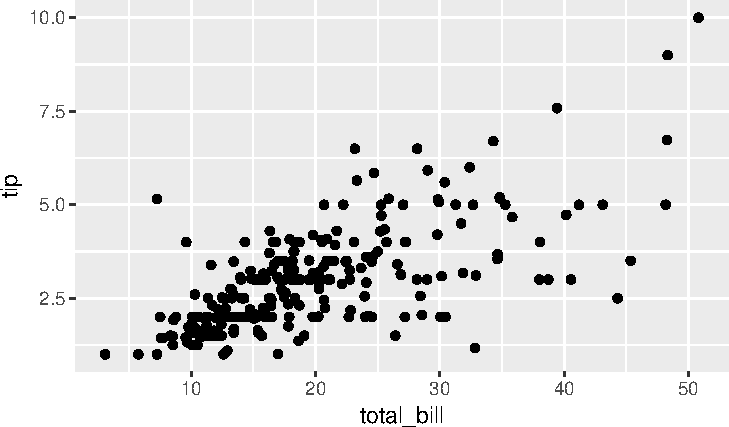
\includegraphics{DatenerhebungStatistik-Uebung_files/figure-latex/unnamed-chunk-160-1.pdf}

Es scheint einen positiven Zusammenhang zu geben. Modellieren wir die
\textbf{abhängige} Variable \texttt{tip} (inhaltliche Entscheidung!) als
lineare Funktion der \textbf{unabhängigen} Variable
\texttt{total\_bill}:

\begin{Shaded}
\begin{Highlighting}[]
\NormalTok{LinMod}\FloatTok{.1}\NormalTok{ <-}\StringTok{ }\KeywordTok{lm}\NormalTok{(tip }\OperatorTok{~}\StringTok{ }\NormalTok{total_bill, }\DataTypeTok{data=}\NormalTok{tips)}
\KeywordTok{summary}\NormalTok{(LinMod}\FloatTok{.1}\NormalTok{)}
\end{Highlighting}
\end{Shaded}

\begin{verbatim}
## 
## Call:
## lm(formula = tip ~ total_bill, data = tips)
## 
## Residuals:
##     Min      1Q  Median      3Q     Max 
## -3.1982 -0.5652 -0.0974  0.4863  3.7434 
## 
## Coefficients:
##             Estimate Std. Error t value Pr(>|t|)    
## (Intercept) 0.920270   0.159735   5.761 2.53e-08 ***
## total_bill  0.105025   0.007365  14.260  < 2e-16 ***
## ---
## Signif. codes:  0 '***' 0.001 '**' 0.01 '*' 0.05 '.' 0.1 ' ' 1
## 
## Residual standard error: 1.022 on 242 degrees of freedom
## Multiple R-squared:  0.4566, Adjusted R-squared:  0.4544 
## F-statistic: 203.4 on 1 and 242 DF,  p-value: < 2.2e-16
\end{verbatim}

Der Achsenabschnitt (\texttt{intercept}) wird mit 0.92 geschätzt, die
Steigung in Richtung \texttt{total\_bill} mit 0.11: steigt
\texttt{total\_bill} um einen Dollar, steigt im \emph{Durchschnitt}
\texttt{tip} um 0.11\(\,\)\$. Die (Punkt-)Prognose für \texttt{tip}
lautet also

\texttt{tip} = 0.92 + 0.11 * \texttt{total\_bill}

Die Koeffzienten werden dabei so geschätzt, dass \(\sum \epsilon_i^2\)
minimiert wird. Dies wird auch als \emph{Kleinste Quadrate}
(\emph{Ordinary Least Squares}, \emph{OLS}) Kriterium bezeichnet. Eine
robuste Regression ist z. B. mit der Funktion \texttt{rlm()} aus dem
Paket \texttt{MASS} möglich.

In mosaic kann ein solches Modell einfach als neue Funktion definiert
werden:

\begin{Shaded}
\begin{Highlighting}[]
\NormalTok{LinMod}\FloatTok{.1}\NormalTok{Fun <-}\StringTok{ }\KeywordTok{makeFun}\NormalTok{(LinMod}\FloatTok{.1}\NormalTok{)}
\end{Highlighting}
\end{Shaded}

Die (Punkt-)Prognose für die Trinkgeldhöhe, bspw. für eine Rechnung von
30\(\,\)\$ kann dann berechnet werden

\begin{Shaded}
\begin{Highlighting}[]
\KeywordTok{LinMod.1Fun}\NormalTok{(}\DataTypeTok{total_bill=}\DecValTok{30}\NormalTok{)}
\end{Highlighting}
\end{Shaded}

\begin{verbatim}
##        1 
## 4.071005
\end{verbatim}

also 4.07\(\,\)\$.

In mosaic kann die Modellgerade über

\begin{Shaded}
\begin{Highlighting}[]
\KeywordTok{plotModel}\NormalTok{(LinMod}\FloatTok{.1}\NormalTok{)}
\end{Highlighting}
\end{Shaded}

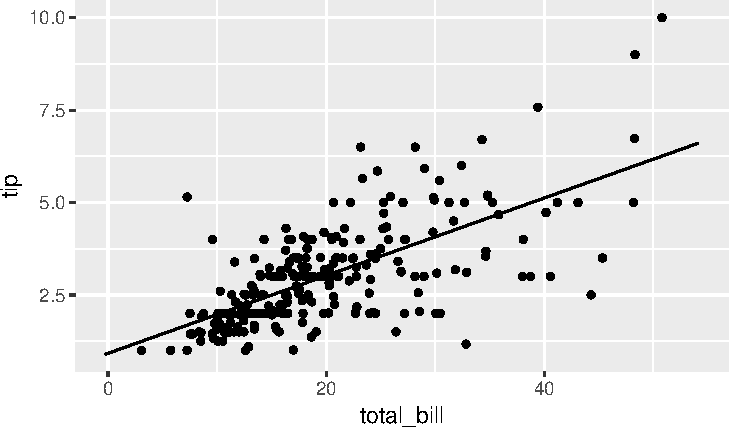
\includegraphics{DatenerhebungStatistik-Uebung_files/figure-latex/unnamed-chunk-164-1.pdf}

betrachtet werden. Das \textbf{Bestimmtheitsmaß}, d.~h. der Anteil der
im Modell erklärten Varianz,
\[R^2=1-\frac{\sum_{i=1}^n (y_i-\hat{y}_i)^2}{\sum_{i=1}^n (y_i-\bar{y})^2}\]
ist mit 0.46 \enquote{ok}: 46\(\,\)\% der Variation des Trinkgeldes wird
im Modell erklärt.

Aber wie sieht es mit den Annahmen aus?

\begin{itemize}
\tightlist
\item
  Die Linearität des Zusammenhangs haben wir zu Beginn mit Hilfe des
  Scatterplots \enquote{überprüft}.
\item
  Zur Überprüfung der Normalverteilung der Residuen zeichnen wir ein
  Histogramm. Die Residuen können über den Befehl \texttt{resid()} aus
  einem Linearen Modell extrahiert werden. Hier scheint es zu passen:
\end{itemize}

\begin{Shaded}
\begin{Highlighting}[]
\KeywordTok{gf_histogram}\NormalTok{( }\OperatorTok{~}\StringTok{ }\KeywordTok{resid}\NormalTok{(LinMod}\FloatTok{.1}\NormalTok{))}
\end{Highlighting}
\end{Shaded}

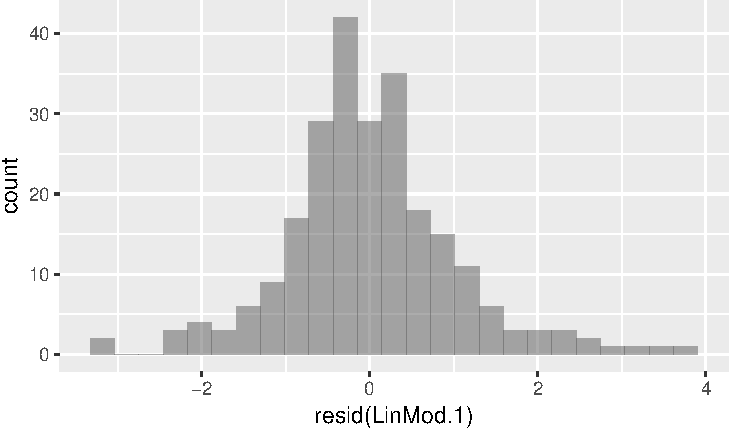
\includegraphics{DatenerhebungStatistik-Uebung_files/figure-latex/unnamed-chunk-165-1.pdf}

\begin{itemize}
\tightlist
\item
  Konstante Varianz: Dies kann z. B. mit einem Scatterplot der Residuen
  auf der y-Achse und den angepassten Werten auf der x-Achse überprüft
  werden. Die angepassten Werte werden über den Befehl \texttt{fitted()}
  extrahiert. Diese Annahme scheint verletzt zu sein (siehe unten): je
  größer die Prognose des Trinkgeldes, desto größer wirkt die Streuung
  der Residuen. Dieses Phänomen ließ sich schon aus dem ursprünglichen
  Scatterplot
  \texttt{xyplot(tip\ \textasciitilde{}\ total\_bill,\ data=tips)}
  erahnen. Das ist auch inhaltlich plausibel: je höher die Rechnung,
  desto höher die Varianz beim Trinkgeld. Die Verletzung dieser Annahme
  beeinflusst \emph{nicht} die Schätzung der Steigung, sondern die
  Schätzung des Standardfehlers, also des p-Wertes des Hypothesentests,
  d.~h., \(H_0:\beta_1=0\).
\end{itemize}

\begin{Shaded}
\begin{Highlighting}[]
\KeywordTok{gf_point}\NormalTok{(}\KeywordTok{resid}\NormalTok{(LinMod}\FloatTok{.1}\NormalTok{) }\OperatorTok{~}\StringTok{ }\KeywordTok{fitted}\NormalTok{(LinMod}\FloatTok{.1}\NormalTok{))}
\end{Highlighting}
\end{Shaded}

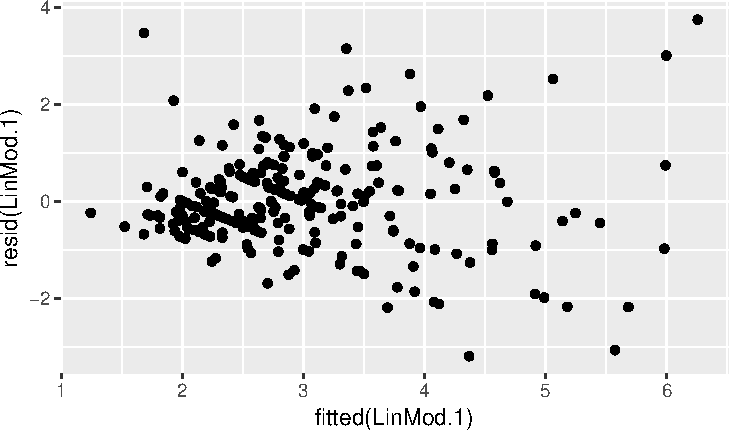
\includegraphics{DatenerhebungStatistik-Uebung_files/figure-latex/unnamed-chunk-166-1.pdf}

\begin{itemize}
\tightlist
\item
  Extreme Ausreißer: Wie am Plot der Linearen Regression
  \texttt{plotModel(LinMod.1)} erkennbar, gibt es vereinzelt Ausreißer
  nach oben, allerdings ohne einen extremen Hebel.
\end{itemize}

Hängt die Rechnungshöhe von der Anzahl der Personen ab? Bestimmt, aber
wie?

\begin{Shaded}
\begin{Highlighting}[]
\KeywordTok{gf_point}\NormalTok{(total_bill }\OperatorTok{~}\StringTok{ }\NormalTok{size, }\DataTypeTok{data=}\NormalTok{tips)}
\end{Highlighting}
\end{Shaded}

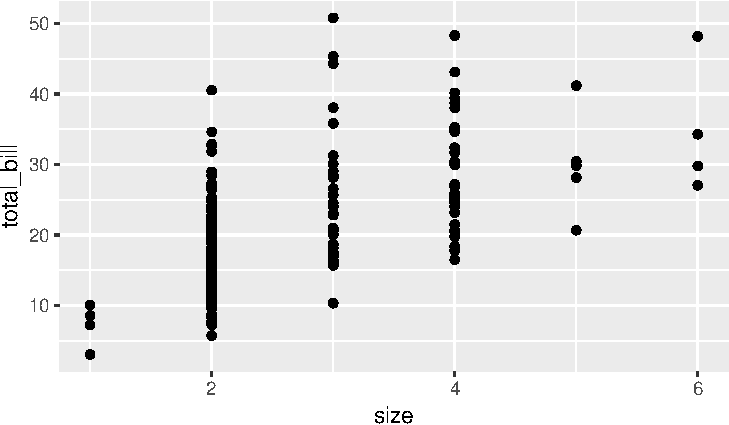
\includegraphics{DatenerhebungStatistik-Uebung_files/figure-latex/unnamed-chunk-167-1.pdf}

Da bei diskreten metrischen Variablen (hier \texttt{size}) Punkte
übereinander liegen können, sollte man \enquote{jittern}, d.~h., eine
(kleine) Zufallszahl addieren:

\begin{Shaded}
\begin{Highlighting}[]
\KeywordTok{set.seed}\NormalTok{(}\DecValTok{1896}\NormalTok{) }\CommentTok{# Zufallszahlengenerater setzen}
\KeywordTok{gf_point}\NormalTok{(total_bill }\OperatorTok{~}\StringTok{ }\KeywordTok{jitter}\NormalTok{(size), }\DataTypeTok{data=}\NormalTok{tips)}
\end{Highlighting}
\end{Shaded}

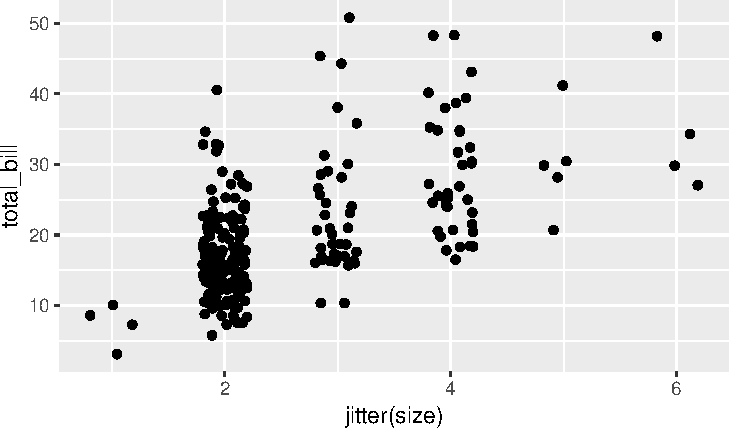
\includegraphics{DatenerhebungStatistik-Uebung_files/figure-latex/unnamed-chunk-168-1.pdf}

\begin{center}\rule{0.5\linewidth}{\linethickness}\end{center}

\textbf{Übung:}

\begin{enumerate}
\def\labelenumi{\arabic{enumi}.}
\tightlist
\item
  Um wie viel Dollar steigt im Durchschnitt das Trinkgeld, wenn eine
  Person mehr am Tisch sitzt?
\item
  Für wie aussagekräftig halten Sie Ihr Ergebnis aus 1.?
\end{enumerate}

\begin{center}\rule{0.5\linewidth}{\linethickness}\end{center}

\hypertarget{regression-mit-kategorialen-werten}{%
\section{Regression mit kategorialen
Werten}\label{regression-mit-kategorialen-werten}}

Der Wochentag \texttt{day} ist eine kategoriale Variable. Wie sieht eine
Regression des Trinkgeldes darauf aus?

Zunächst grafisch:

\begin{Shaded}
\begin{Highlighting}[]
\KeywordTok{gf_point}\NormalTok{(tip }\OperatorTok{~}\StringTok{ }\NormalTok{day, }\DataTypeTok{data=}\NormalTok{tips)}
\end{Highlighting}
\end{Shaded}

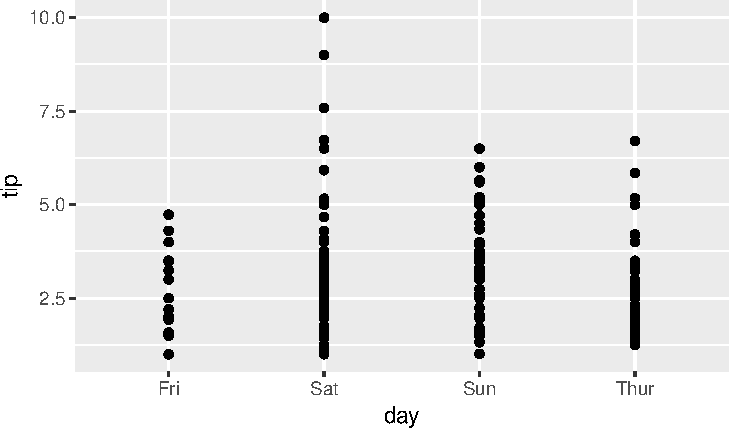
\includegraphics{DatenerhebungStatistik-Uebung_files/figure-latex/unnamed-chunk-169-1.pdf}

Und als Lineares Modell:

\begin{Shaded}
\begin{Highlighting}[]
\NormalTok{LinMod}\FloatTok{.2}\NormalTok{ <-}\StringTok{ }\KeywordTok{lm}\NormalTok{(tip }\OperatorTok{~}\StringTok{ }\NormalTok{day, }\DataTypeTok{data=}\NormalTok{tips)}
\KeywordTok{summary}\NormalTok{(LinMod}\FloatTok{.2}\NormalTok{)}
\end{Highlighting}
\end{Shaded}

\begin{verbatim}
## 
## Call:
## lm(formula = tip ~ day, data = tips)
## 
## Residuals:
##     Min      1Q  Median      3Q     Max 
## -2.2451 -0.9931 -0.2347  0.5382  7.0069 
## 
## Coefficients:
##             Estimate Std. Error t value Pr(>|t|)    
## (Intercept)  2.73474    0.31612   8.651 7.46e-16 ***
## daySat       0.25837    0.34893   0.740    0.460    
## daySun       0.52039    0.35343   1.472    0.142    
## dayThur      0.03671    0.36132   0.102    0.919    
## ---
## Signif. codes:  0 '***' 0.001 '**' 0.01 '*' 0.05 '.' 0.1 ' ' 1
## 
## Residual standard error: 1.378 on 240 degrees of freedom
## Multiple R-squared:  0.02048,    Adjusted R-squared:  0.008232 
## F-statistic: 1.672 on 3 and 240 DF,  p-value: 0.1736
\end{verbatim}

Die im Modell angegebenen Schätzwerte sind die Änderung der
Trinkgeldprognose, wenn z. B. der Tag ein Samstag (\texttt{daySat}) im
Vergleich zu einer Referenzkategorie. Dies ist in R das erste Element
des Vektors der Faktorlevel. Welcher dies ist ist über den Befehl
\texttt{levels()} zu erfahren

\begin{Shaded}
\begin{Highlighting}[]
\KeywordTok{levels}\NormalTok{(tips}\OperatorTok{$}\NormalTok{day)}
\end{Highlighting}
\end{Shaded}

\begin{verbatim}
## [1] "Fri"  "Sat"  "Sun"  "Thur"
\end{verbatim}

hier also Fri (aufgrund der standardmäßig aufsteigenden alphanumerischen
Sortierung). Dies kann über \texttt{relevel()} geändert werden. Soll z.
B. die Referenz der Donnerstag, \texttt{Thur} sein:

\begin{Shaded}
\begin{Highlighting}[]
\NormalTok{tips}\OperatorTok{$}\NormalTok{day <-}\StringTok{ }\KeywordTok{relevel}\NormalTok{(tips}\OperatorTok{$}\NormalTok{day, }\DataTypeTok{ref =} \StringTok{"Thur"}\NormalTok{)}
\KeywordTok{levels}\NormalTok{(tips}\OperatorTok{$}\NormalTok{day)}
\end{Highlighting}
\end{Shaded}

\begin{verbatim}
## [1] "Thur" "Fri"  "Sat"  "Sun"
\end{verbatim}

Das Modell ändert sich entsprechend:

\begin{Shaded}
\begin{Highlighting}[]
\NormalTok{LinMod}\FloatTok{.3}\NormalTok{ <-}\StringTok{ }\KeywordTok{lm}\NormalTok{(tip }\OperatorTok{~}\StringTok{ }\NormalTok{day, }\DataTypeTok{data=}\NormalTok{tips)}
\KeywordTok{summary}\NormalTok{(LinMod}\FloatTok{.3}\NormalTok{)}
\end{Highlighting}
\end{Shaded}

\begin{verbatim}
## 
## Call:
## lm(formula = tip ~ day, data = tips)
## 
## Residuals:
##     Min      1Q  Median      3Q     Max 
## -2.2451 -0.9931 -0.2347  0.5382  7.0069 
## 
## Coefficients:
##             Estimate Std. Error t value Pr(>|t|)    
## (Intercept)  2.77145    0.17500  15.837   <2e-16 ***
## dayFri      -0.03671    0.36132  -0.102   0.9191    
## daySat       0.22165    0.22902   0.968   0.3341    
## daySun       0.48368    0.23581   2.051   0.0413 *  
## ---
## Signif. codes:  0 '***' 0.001 '**' 0.01 '*' 0.05 '.' 0.1 ' ' 1
## 
## Residual standard error: 1.378 on 240 degrees of freedom
## Multiple R-squared:  0.02048,    Adjusted R-squared:  0.008232 
## F-statistic: 1.672 on 3 and 240 DF,  p-value: 0.1736
\end{verbatim}

sowie als Plot:

\begin{Shaded}
\begin{Highlighting}[]
\KeywordTok{plotModel}\NormalTok{(LinMod}\FloatTok{.3}\NormalTok{)}
\end{Highlighting}
\end{Shaded}

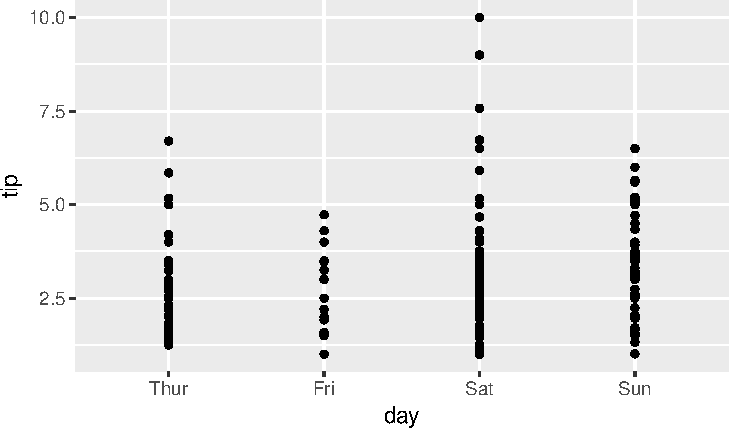
\includegraphics{DatenerhebungStatistik-Uebung_files/figure-latex/unnamed-chunk-174-1.pdf}

Eine Alternative zu \texttt{relevel()} zur Bestimmung der
Referenzkategorie ist es, innerhalb von \texttt{factor()} die Option
\texttt{levels=} direkt in der gewünschten Sortierung zu setzen.

\begin{Shaded}
\begin{Highlighting}[]
\NormalTok{day <-}\StringTok{ }\KeywordTok{factor}\NormalTok{(tips}\OperatorTok{$}\NormalTok{day, }\DataTypeTok{levels=}\KeywordTok{c}\NormalTok{(}\StringTok{"Thur"}\NormalTok{, }\StringTok{"Fri"}\NormalTok{, }\StringTok{"Sat"}\NormalTok{,  }\StringTok{"Sun"}\NormalTok{))}
\end{Highlighting}
\end{Shaded}

Die (Punkt-)Prognose für die Trinkgeldhöhe, bspw. an einen Freitag kann
dann berechnet werden

\begin{Shaded}
\begin{Highlighting}[]
\NormalTok{LinMod}\FloatTok{.3}\NormalTok{Fun <-}\StringTok{ }\KeywordTok{makeFun}\NormalTok{(LinMod}\FloatTok{.3}\NormalTok{)}
\KeywordTok{LinMod.3Fun}\NormalTok{(}\DataTypeTok{day=}\StringTok{"Fri"}\NormalTok{)}
\end{Highlighting}
\end{Shaded}

\begin{verbatim}
##        1 
## 2.734737
\end{verbatim}

\begin{center}\rule{0.5\linewidth}{\linethickness}\end{center}

\textbf{Übung:}

\begin{enumerate}
\def\labelenumi{\arabic{enumi}.}
\setcounter{enumi}{2}
\tightlist
\item
  Wie verändert sich die Rechnungshöhe im Durchschnitt, wenn die
  Essenszeit Dinner statt Lunch ist?
\item
  Wie viel \% der Variation der Rechnungshöhe können Sie durch die
  Essenszeit modellieren?
\end{enumerate}

\begin{center}\rule{0.5\linewidth}{\linethickness}\end{center}

\hypertarget{multivariate-regression}{%
\section{Multivariate Regression}\label{multivariate-regression}}

Aber wie wirken sich die Einflussgrößen \emph{zusammen} auf das
Trinkgeld aus?

\begin{Shaded}
\begin{Highlighting}[]
\NormalTok{LinMod}\FloatTok{.4}\NormalTok{ <-}\StringTok{ }\KeywordTok{lm}\NormalTok{(tip }\OperatorTok{~}\StringTok{ }\NormalTok{total_bill }\OperatorTok{+}\StringTok{ }\NormalTok{size }\OperatorTok{+}\StringTok{ }\NormalTok{sex  }\OperatorTok{+}\StringTok{ }\NormalTok{smoker }\OperatorTok{+}\StringTok{ }\NormalTok{day }\OperatorTok{+}\StringTok{ }\NormalTok{time, }\DataTypeTok{data=}\NormalTok{tips)}
\KeywordTok{summary}\NormalTok{(LinMod}\FloatTok{.4}\NormalTok{)}
\end{Highlighting}
\end{Shaded}

\begin{verbatim}
## 
## Call:
## lm(formula = tip ~ total_bill + size + sex + smoker + day + time, 
##     data = tips)
## 
## Residuals:
##     Min      1Q  Median      3Q     Max 
## -2.8475 -0.5729 -0.1026  0.4756  4.1076 
## 
## Coefficients:
##              Estimate Std. Error t value Pr(>|t|)    
## (Intercept)  0.641558   0.497586   1.289   0.1985    
## total_bill   0.094487   0.009601   9.841   <2e-16 ***
## size         0.175992   0.089528   1.966   0.0505 .  
## sexMale     -0.032441   0.141612  -0.229   0.8190    
## smokerYes   -0.086408   0.146587  -0.589   0.5561    
## dayFri       0.162259   0.393405   0.412   0.6804    
## daySat       0.040801   0.470604   0.087   0.9310    
## daySun       0.136779   0.471696   0.290   0.7721    
## timeLunch    0.068129   0.444617   0.153   0.8783    
## ---
## Signif. codes:  0 '***' 0.001 '**' 0.01 '*' 0.05 '.' 0.1 ' ' 1
## 
## Residual standard error: 1.024 on 235 degrees of freedom
## Multiple R-squared:  0.4701, Adjusted R-squared:  0.452 
## F-statistic: 26.06 on 8 and 235 DF,  p-value: < 2.2e-16
\end{verbatim}

Interessant sind die negativen Vorzeichen vor den Schätzwerten für
\texttt{sexMale} und \texttt{smokerYes} -- anscheinend geben Männer und
Raucher weniger Trinkgeld, wenn alle anderen Faktoren konstant bleiben.
Bei einer rein univariaten Betrachtung wäre etwas anderes
herausgekommen.

\begin{Shaded}
\begin{Highlighting}[]
\KeywordTok{summary}\NormalTok{(}\KeywordTok{lm}\NormalTok{(tip }\OperatorTok{~}\StringTok{ }\NormalTok{sex, }\DataTypeTok{data=}\NormalTok{tips))}
\end{Highlighting}
\end{Shaded}

\begin{verbatim}
## 
## Call:
## lm(formula = tip ~ sex, data = tips)
## 
## Residuals:
##     Min      1Q  Median      3Q     Max 
## -2.0896 -1.0896 -0.0896  0.6666  6.9104 
## 
## Coefficients:
##             Estimate Std. Error t value Pr(>|t|)    
## (Intercept)   2.8334     0.1481  19.137   <2e-16 ***
## sexMale       0.2562     0.1846   1.388    0.166    
## ---
## Signif. codes:  0 '***' 0.001 '**' 0.01 '*' 0.05 '.' 0.1 ' ' 1
## 
## Residual standard error: 1.381 on 242 degrees of freedom
## Multiple R-squared:  0.007896,   Adjusted R-squared:  0.003797 
## F-statistic: 1.926 on 1 and 242 DF,  p-value: 0.1665
\end{verbatim}

\begin{Shaded}
\begin{Highlighting}[]
\KeywordTok{summary}\NormalTok{(}\KeywordTok{lm}\NormalTok{(tip }\OperatorTok{~}\StringTok{ }\NormalTok{smoker, }\DataTypeTok{data=}\NormalTok{tips))}
\end{Highlighting}
\end{Shaded}

\begin{verbatim}
## 
## Call:
## lm(formula = tip ~ smoker, data = tips)
## 
## Residuals:
##     Min      1Q  Median      3Q     Max 
## -2.0087 -0.9936 -0.1003  0.5580  6.9913 
## 
## Coefficients:
##             Estimate Std. Error t value Pr(>|t|)    
## (Intercept)  2.99185    0.11283  26.517   <2e-16 ***
## smokerYes    0.01686    0.18276   0.092    0.927    
## ---
## Signif. codes:  0 '***' 0.001 '**' 0.01 '*' 0.05 '.' 0.1 ' ' 1
## 
## Residual standard error: 1.386 on 242 degrees of freedom
## Multiple R-squared:  3.515e-05,  Adjusted R-squared:  -0.004097 
## F-statistic: 0.008506 on 1 and 242 DF,  p-value: 0.9266
\end{verbatim}

Diese \emph{Umkehrung} des modellierten Effektes liegt daran, dass es
auch einen positiven Zusammenhang zur Rechnungshöhe gibt:

\begin{Shaded}
\begin{Highlighting}[]
\KeywordTok{summary}\NormalTok{(}\KeywordTok{lm}\NormalTok{(total_bill }\OperatorTok{~}\StringTok{ }\NormalTok{sex, }\DataTypeTok{data=}\NormalTok{tips))}
\end{Highlighting}
\end{Shaded}

\begin{verbatim}
## 
## Call:
## lm(formula = total_bill ~ sex, data = tips)
## 
## Residuals:
##    Min     1Q Median     3Q    Max 
## -14.99  -6.02  -1.94   3.99  30.07 
## 
## Coefficients:
##             Estimate Std. Error t value Pr(>|t|)    
## (Intercept)  18.0569     0.9463  19.081   <2e-16 ***
## sexMale       2.6872     1.1797   2.278   0.0236 *  
## ---
## Signif. codes:  0 '***' 0.001 '**' 0.01 '*' 0.05 '.' 0.1 ' ' 1
## 
## Residual standard error: 8.827 on 242 degrees of freedom
## Multiple R-squared:  0.02099,    Adjusted R-squared:  0.01694 
## F-statistic: 5.188 on 1 and 242 DF,  p-value: 0.02361
\end{verbatim}

\begin{Shaded}
\begin{Highlighting}[]
\KeywordTok{summary}\NormalTok{(}\KeywordTok{lm}\NormalTok{(total_bill }\OperatorTok{~}\StringTok{ }\NormalTok{smoker, }\DataTypeTok{data=}\NormalTok{tips))}
\end{Highlighting}
\end{Shaded}

\begin{verbatim}
## 
## Call:
## lm(formula = total_bill ~ smoker, data = tips)
## 
## Residuals:
##     Min      1Q  Median      3Q     Max 
## -17.686  -6.459  -1.888   4.583  30.054 
## 
## Coefficients:
##             Estimate Std. Error t value Pr(>|t|)    
## (Intercept)  19.1883     0.7233  26.529   <2e-16 ***
## smokerYes     1.5681     1.1716   1.338    0.182    
## ---
## Signif. codes:  0 '***' 0.001 '**' 0.01 '*' 0.05 '.' 0.1 ' ' 1
## 
## Residual standard error: 8.888 on 242 degrees of freedom
## Multiple R-squared:  0.007348,   Adjusted R-squared:  0.003246 
## F-statistic: 1.791 on 1 and 242 DF,  p-value: 0.182
\end{verbatim}

Im vollem Modell \texttt{LinMod.4} sind alle unabhängigen Variablen
berücksichtigt, die Koeffizienten beziehen sich dann immer auf: gegeben,
die anderen Variablen bleiben konstant, d.~h. ceteris paribus.

Vergleichen wir mal zwei Modelle:

\begin{Shaded}
\begin{Highlighting}[]
\NormalTok{LinMod}\FloatTok{.5}\NormalTok{a <-}\StringTok{ }\KeywordTok{lm}\NormalTok{(tip }\OperatorTok{~}\StringTok{  }\NormalTok{sex, }\DataTypeTok{data=}\NormalTok{tips)}
\KeywordTok{coef}\NormalTok{(LinMod}\FloatTok{.5}\NormalTok{a) }\CommentTok{# Koeffizienten extrahieren}
\end{Highlighting}
\end{Shaded}

\begin{verbatim}
## (Intercept)     sexMale 
##   2.8334483   0.2561696
\end{verbatim}

\begin{Shaded}
\begin{Highlighting}[]
\NormalTok{LinMod}\FloatTok{.5}\NormalTok{b <-}\StringTok{ }\KeywordTok{lm}\NormalTok{(tip }\OperatorTok{~}\StringTok{  }\NormalTok{sex }\OperatorTok{+}\StringTok{ }\NormalTok{total_bill, }\DataTypeTok{data=}\NormalTok{tips)}
\KeywordTok{coef}\NormalTok{(LinMod}\FloatTok{.5}\NormalTok{b) }\CommentTok{# Koeffizienten extrahieren}
\end{Highlighting}
\end{Shaded}

\begin{verbatim}
## (Intercept)     sexMale  total_bill 
##  0.93327849 -0.02660871  0.10523236
\end{verbatim}

Ohne die Berücksichtigung der \textbf{Kovariable/Störvariable}
Rechnungshöhe geben \texttt{Male} ein um im Durchschnitt 0.26\(\,\)\$
\emph{höheres} Trinkgeld, bei Kontrolle, d.~h. gleicher Rechnungshöhe,
ein um 0.03\(\,\)\$ \emph{niedrigeres} Trinkgeld als die Referenzklasse
\texttt{Female} (\texttt{levels(tips\$sex){[}1{]}}).

\hypertarget{inferenz-in-der-linearen-regression}{%
\section{Inferenz in der linearen
Regression}\label{inferenz-in-der-linearen-regression}}

Kehren wir noch einmal zur multivariaten Regression (\texttt{LinMod.4})
zurück.

\begin{Shaded}
\begin{Highlighting}[]
\KeywordTok{summary}\NormalTok{(LinMod}\FloatTok{.4}\NormalTok{)}
\end{Highlighting}
\end{Shaded}

\begin{verbatim}
## 
## Call:
## lm(formula = tip ~ total_bill + size + sex + smoker + day + time, 
##     data = tips)
## 
## Residuals:
##     Min      1Q  Median      3Q     Max 
## -2.8475 -0.5729 -0.1026  0.4756  4.1076 
## 
## Coefficients:
##              Estimate Std. Error t value Pr(>|t|)    
## (Intercept)  0.641558   0.497586   1.289   0.1985    
## total_bill   0.094487   0.009601   9.841   <2e-16 ***
## size         0.175992   0.089528   1.966   0.0505 .  
## sexMale     -0.032441   0.141612  -0.229   0.8190    
## smokerYes   -0.086408   0.146587  -0.589   0.5561    
## dayFri       0.162259   0.393405   0.412   0.6804    
## daySat       0.040801   0.470604   0.087   0.9310    
## daySun       0.136779   0.471696   0.290   0.7721    
## timeLunch    0.068129   0.444617   0.153   0.8783    
## ---
## Signif. codes:  0 '***' 0.001 '**' 0.01 '*' 0.05 '.' 0.1 ' ' 1
## 
## Residual standard error: 1.024 on 235 degrees of freedom
## Multiple R-squared:  0.4701, Adjusted R-squared:  0.452 
## F-statistic: 26.06 on 8 and 235 DF,  p-value: < 2.2e-16
\end{verbatim}

In der 4. Spalte der mit Zeilennamen versehenen Tabelle
\texttt{Coefficients} stehen die p-Werte der Nullhypothese, die
unabhängige Variable hat, gegeben alle anderen Variablen im Modell,
keinen linearen Einfluss auf die abhängige Variable: \(H_0: \beta_i=0\).
Zur Bestimmung des p-Wertes wird der Schätzer (\texttt{Estimate}) durch
den Standardfehler (\texttt{Std.\ Error}) dividiert. Der resultierende
t-Wert (\texttt{t\ value}) wird dann, zusammen mit der Anzahl an
Freiheitsgraden zur Berechnung des p-Wertes
(\texttt{Pr(\textgreater{}\textbar{}t\textbar{})}) verwendet. Ein
einfacher t-Test!

Zur schnelleren Übersicht finden sich dahinter \enquote{Sternchen} und
\enquote{Punkte}, die die entsprechenden Signifikanzniveaus
symbolisieren: \texttt{***} bedeutet eine Irrtumswahrscheinlichkeit,
Wahrscheinlichkeit für Fehler 1. Art, von unter 0.001, d.~h. unter
0,1\(\,\)\%. \texttt{**} entsprechend 1\(\,\)\%, \texttt{*} 5\(\,\)\%
und \texttt{.} 10\(\,\)\%.

Zum Signifikanzniveau von 10\(\,\)\% sind hier also zwei Faktoren
signifikant -- nicht notwendigerweise relevant: Rechnungshöhe
\texttt{total\_bill} sowie Anzahl Personen \texttt{size}. Beides wirkt
sich linear positiv auf die Trinkgeldhöhe aus: Mit jedem Dollar
Rechnungshöhe steigt im Mittelwert die Trinkgeldhöhe um 0.09 Dollar, mit
jeder Person um 0.18 Dollar -- gegeben alle anderen Faktoren bleiben
konstant. Das Bestimmtheitsmaß R\textsuperscript{2}
(\texttt{Multiple\ R-squared:}) liegt bei 0.47, also 47\(\,\)\% der
Variation des Trinkgeldes wird im Modell erklärt.

Außerdem wird getestet, ob alle Koeffizienten der unabhängigen Variablen
gleich Null sind: \[H_0: \beta_1=\beta_2=\cdots=\beta_k=0\] Das Ergebnis
des zugrundeliegenden F-Tests (vgl. Varianzanalyse) wird in der letzten
Zeile angegeben (\texttt{F-Statistic}). Hier wird \(H_0\) also
verworfen.

\hypertarget{erweiterungen}{%
\section{Erweiterungen}\label{erweiterungen}}

\hypertarget{modellwahl}{%
\subsection{Modellwahl}\label{modellwahl}}

Das Modell mit allen Variablen des Datensatzes, d.~h. mit 6 unabhängigen
(\texttt{LinMod.4}), erklärt 47.01\(\,\)\% der Variation, das Modell
\emph{nur} mit der Rechnungshöhe als erklärende Variable
(\texttt{LinMod.1}) schon 45.66\(\,\)\%, der Erklärungszuwachs liegt
also gerade einmal bei 1.35 Prozentpunkten. In der Statistik ist die
Wahl des \emph{richtigen} Modells eine der größten Herausforderungen,
auch deshalb, weil das wahre Modell in der Regel nicht bekannt ist und
es schwer ist, die richtige Balance zwischen Einfachheit und Komplexität
zu finden. Aufgrund des Zufalls kann es immer passieren, dass das Modell
sich zu sehr an die \emph{zufälligen} Daten anpasst (Stichwort:
Overfitting). Es gibt unzählige Modellwahlmethoden, und leider
garantiert keine, dass immer das beste Modell gefunden wird. Eine
Möglichkeit ist die sogenannte Schrittweise-Rückwärtsselektion auf Basis
des Akaike-Informationskriteriums (AIC)\footnote{siehe z. B. Rob J
  Hyndman \& George Athanasopoulos, Forecasting: principles and
  practice, Kapitel 5.3: Selecting predictors,
  \url{https://www.otexts.org/fpp/5/3}}. Diese ist nicht nur recht weit
verbreitet -- und liefert unter bestimmten Annahmen das
\enquote{richtige} Modell -- sondern in R durch den Befehl
\texttt{step()} einfach umsetzbar:

\begin{Shaded}
\begin{Highlighting}[]
\KeywordTok{step}\NormalTok{(LinMod}\FloatTok{.4}\NormalTok{)}
\end{Highlighting}
\end{Shaded}

\begin{verbatim}
## Start:  AIC=20.51
## tip ~ total_bill + size + sex + smoker + day + time
## 
##              Df Sum of Sq    RSS     AIC
## - day         3     0.609 247.14  15.116
## - time        1     0.025 246.55  18.538
## - sex         1     0.055 246.58  18.568
## - smoker      1     0.365 246.89  18.874
## <none>                    246.53  20.513
## - size        1     4.054 250.58  22.493
## - total_bill  1   101.595 348.12 102.713
## 
## Step:  AIC=15.12
## tip ~ total_bill + size + sex + smoker + time
## 
##              Df Sum of Sq    RSS    AIC
## - time        1     0.001 247.14 13.117
## - sex         1     0.042 247.18 13.157
## - smoker      1     0.380 247.52 13.490
## <none>                    247.14 15.116
## - size        1     4.341 251.48 17.365
## - total_bill  1   101.726 348.86 97.232
## 
## Step:  AIC=13.12
## tip ~ total_bill + size + sex + smoker
## 
##              Df Sum of Sq    RSS    AIC
## - sex         1     0.041 247.18 11.157
## - smoker      1     0.379 247.52 11.491
## <none>                    247.14 13.117
## - size        1     4.342 251.48 15.366
## - total_bill  1   103.327 350.46 96.350
## 
## Step:  AIC=11.16
## tip ~ total_bill + size + smoker
## 
##              Df Sum of Sq    RSS    AIC
## - smoker      1     0.376 247.55  9.528
## <none>                    247.18 11.157
## - size        1     4.344 251.52 13.408
## - total_bill  1   104.263 351.44 95.029
## 
## Step:  AIC=9.53
## tip ~ total_bill + size
## 
##              Df Sum of Sq    RSS    AIC
## <none>                    247.55  9.528
## - size        1     5.235 252.79 12.634
## - total_bill  1   106.281 353.83 94.685
\end{verbatim}

\begin{verbatim}
## 
## Call:
## lm(formula = tip ~ total_bill + size, data = tips)
## 
## Coefficients:
## (Intercept)   total_bill         size  
##     0.66894      0.09271      0.19260
\end{verbatim}

In den letzten Zeilen der Ausgabe steht das beste Modell, das diese
Methode (schrittweise, rückwärts) mit diesem Kriterium (AIC) bei diesen
Daten findet (Punktprognose, d.~h. ohne Residuum):

\texttt{tip\ =\ 0.66894\ +\ 0.09271\ *\ total\_bill\ +\ 0.1926\ *\ size}

Der Ausgabe können Sie auch entnehmen, welche Variablen in welcher
Reihenfolge \emph{entfernt} wurden: Zunächst \texttt{day}, dann
\texttt{time}, danach \texttt{sex} und schließlich \texttt{smoker}. Hier
sind also dieselben Variablen noch im Modell, die auch in
\texttt{LinMod.4} signifikant zum Niveau 10\(\,\)\% waren, eine Auswahl
der dort signifikanten Variablen hätte also dasselbe Modell ergeben. Das
ist häufig so, aber nicht immer!

\hypertarget{interaktionen}{%
\subsection{Interaktionen}\label{interaktionen}}

Wir haben gesehen, dass es einen Zusammenhang zwischen der Trinkgeldhöhe
und der Rechnungshöhe gibt. Vielleicht unterscheidet sich der
Zusammenhang je nachdem, ob geraucht wurde, d.~h., vielleicht gibt es
eine Interaktion (Wechselwirkung). Die kann in \texttt{lm} einfach durch
ein \texttt{*} zwischen den unabhängigen Variablen modelliert werden
(\texttt{a*b} entspricht in R Formeln \texttt{a+b+a:b}):

\begin{Shaded}
\begin{Highlighting}[]
\NormalTok{LinMod}\FloatTok{.6}\NormalTok{ <-}\StringTok{ }\KeywordTok{lm}\NormalTok{(tip }\OperatorTok{~}\StringTok{ }\NormalTok{smoker}\OperatorTok{*}\NormalTok{total_bill, }\DataTypeTok{data =}\NormalTok{ tips)}
\KeywordTok{summary}\NormalTok{(LinMod}\FloatTok{.6}\NormalTok{)}
\end{Highlighting}
\end{Shaded}

\begin{verbatim}
## 
## Call:
## lm(formula = tip ~ smoker * total_bill, data = tips)
## 
## Residuals:
##     Min      1Q  Median      3Q     Max 
## -2.6789 -0.5238 -0.1205  0.4749  4.8999 
## 
## Coefficients:
##                       Estimate Std. Error t value Pr(>|t|)    
## (Intercept)           0.360069   0.202058   1.782 0.076012 .  
## smokerYes             1.204203   0.312263   3.856 0.000148 ***
## total_bill            0.137156   0.009678  14.172  < 2e-16 ***
## smokerYes:total_bill -0.067566   0.014189  -4.762 3.32e-06 ***
## ---
## Signif. codes:  0 '***' 0.001 '**' 0.01 '*' 0.05 '.' 0.1 ' ' 1
## 
## Residual standard error: 0.9785 on 240 degrees of freedom
## Multiple R-squared:  0.506,  Adjusted R-squared:  0.4998 
## F-statistic: 81.95 on 3 and 240 DF,  p-value: < 2.2e-16
\end{verbatim}

Der Schätzwert für die Interaktion steht bei \texttt{:}. Hier also: Wenn
geraucht wurde, ist die Steigung im Durchschnitt um 6,8 Cent geringer.
Aber wenn geraucht wurde, ist die Rechnung im Achsenabschnitt erstmal um
1,20\(\,\)\$ höher (Effekt, ceteris paribus). Wer will, kann ausrechnen,
ab welcher Rechnungshöhe Rauchertische im Mittelwert lukrativer sind
\dots 

Das gleiche Bild (höherer Achsenabschnitt, geringere Steigung) ergibt
sich übrigens bei getrennten Regressionen:

\begin{Shaded}
\begin{Highlighting}[]
\KeywordTok{lm}\NormalTok{(tip}\OperatorTok{~}\NormalTok{total_bill, }\DataTypeTok{data=}\NormalTok{tips, }\DataTypeTok{subset =}\NormalTok{ smoker}\OperatorTok{==}\StringTok{"Yes"}\NormalTok{)}
\end{Highlighting}
\end{Shaded}

\begin{verbatim}
## 
## Call:
## lm(formula = tip ~ total_bill, data = tips, subset = smoker == 
##     "Yes")
## 
## Coefficients:
## (Intercept)   total_bill  
##     1.56427      0.06959
\end{verbatim}

\begin{Shaded}
\begin{Highlighting}[]
\KeywordTok{lm}\NormalTok{(tip}\OperatorTok{~}\NormalTok{total_bill, }\DataTypeTok{data=}\NormalTok{tips, }\DataTypeTok{subset =}\NormalTok{ smoker}\OperatorTok{==}\StringTok{"No"}\NormalTok{)}
\end{Highlighting}
\end{Shaded}

\begin{verbatim}
## 
## Call:
## lm(formula = tip ~ total_bill, data = tips, subset = smoker == 
##     "No")
## 
## Coefficients:
## (Intercept)   total_bill  
##      0.3601       0.1372
\end{verbatim}

\hypertarget{weitere-modellierungsmoglichkeiten}{%
\subsection{Weitere
Modellierungsmöglichkeiten}\label{weitere-modellierungsmoglichkeiten}}

Über das Formelinterface \texttt{y\textasciitilde{}x} können auch direkt
z. B. Polynome modelliert werden. Hier eine quadratische Funktion:

\begin{Shaded}
\begin{Highlighting}[]
\KeywordTok{summary}\NormalTok{(}\KeywordTok{lm}\NormalTok{(tip}\OperatorTok{~}\KeywordTok{I}\NormalTok{(total_bill}\OperatorTok{^}\DecValTok{2}\NormalTok{)}\OperatorTok{+}\NormalTok{total_bill, }\DataTypeTok{data=}\NormalTok{tips))}
\end{Highlighting}
\end{Shaded}

\begin{verbatim}
## 
## Call:
## lm(formula = tip ~ I(total_bill^2) + total_bill, data = tips)
## 
## Residuals:
##     Min      1Q  Median      3Q     Max 
## -3.2005 -0.5586 -0.0979  0.4838  3.7762 
## 
## Coefficients:
##                   Estimate Std. Error t value Pr(>|t|)    
## (Intercept)      0.8911170  0.3467554   2.570 0.010776 *  
## I(total_bill^2) -0.0000571  0.0006025  -0.095 0.924573    
## total_bill       0.1078555  0.0307696   3.505 0.000544 ***
## ---
## Signif. codes:  0 '***' 0.001 '**' 0.01 '*' 0.05 '.' 0.1 ' ' 1
## 
## Residual standard error: 1.024 on 241 degrees of freedom
## Multiple R-squared:  0.4566, Adjusted R-squared:  0.4521 
## F-statistic: 101.3 on 2 and 241 DF,  p-value: < 2.2e-16
\end{verbatim}

D. h., die geschätzte Funktion ist eine \enquote{umgedrehte Parabel}
(negatives Vorzeichen bei \texttt{I(total\_bill\^{}2)}), bzw. die
Funktion ist konkav, die Steigung nimmt ab. Allerdings ist der Effekt
nicht signifikant. \textbf{Hinweis:} Um zu \enquote{rechnen} und nicht
beispielsweise Interaktion zu modellieren, geben Sie die Variablen in
der Formel in der Funktion \texttt{I()} (\emph{As Is}) ein.

\hypertarget{prognoseintervalle}{%
\subsection{Prognoseintervalle}\label{prognoseintervalle}}

Insgesamt haben wir viel \enquote{Unsicherheit} u. a. aufgrund von
Variabilität in den Beobachtungen und in den Schätzungen. Wie wirken
sich diese auf die Prognose aus?

Dazu können wir über die Funktion \texttt{predict} Prognoseintervalle
berechnen -- hier für das einfache Modell \texttt{LinMod.1}:

\begin{Shaded}
\begin{Highlighting}[]
\NormalTok{newdat <-}\StringTok{ }\KeywordTok{data.frame}\NormalTok{(}\DataTypeTok{total_bill =} \KeywordTok{seq}\NormalTok{(}\DecValTok{0}\NormalTok{, }\DecValTok{75}\NormalTok{))}
\NormalTok{preddat <-}\StringTok{ }\KeywordTok{predict}\NormalTok{(LinMod}\FloatTok{.1}\NormalTok{, }\DataTypeTok{newdata =}\NormalTok{ newdat, }\DataTypeTok{interval =} \StringTok{"prediction"}\NormalTok{)}
\KeywordTok{head}\NormalTok{(preddat)}
\end{Highlighting}
\end{Shaded}

\begin{verbatim}
##         fit        lwr      upr
## 1 0.9202696 -1.1174151 2.957954
## 2 1.0252941 -1.0103977 3.060986
## 3 1.1303186 -0.9034818 3.164119
## 4 1.2353432 -0.7966677 3.267354
## 5 1.3403677 -0.6899557 3.370691
## 6 1.4453922 -0.5833461 3.474130
\end{verbatim}

\begin{Shaded}
\begin{Highlighting}[]
\KeywordTok{tail}\NormalTok{(preddat)}
\end{Highlighting}
\end{Shaded}

\begin{verbatim}
##         fit      lwr      upr
## 71 8.271986 6.127124 10.41685
## 72 8.377010 6.227178 10.52684
## 73 8.482035 6.327145 10.63692
## 74 8.587059 6.427028 10.74709
## 75 8.692084 6.526825 10.85734
## 76 8.797108 6.626538 10.96768
\end{verbatim}

\begin{Shaded}
\begin{Highlighting}[]
\KeywordTok{matplot}\NormalTok{(newdat}\OperatorTok{$}\NormalTok{total_bill, preddat, }\DataTypeTok{lty =} \KeywordTok{c}\NormalTok{(}\DecValTok{1}\NormalTok{,}\DecValTok{2}\NormalTok{,}\DecValTok{2}\NormalTok{), }\DataTypeTok{type=}\StringTok{"l"}\NormalTok{ )}
\KeywordTok{points}\NormalTok{(}\DataTypeTok{x=}\NormalTok{tips}\OperatorTok{$}\NormalTok{total_bill, }\DataTypeTok{y=}\NormalTok{tips}\OperatorTok{$}\NormalTok{tip)}
\end{Highlighting}
\end{Shaded}

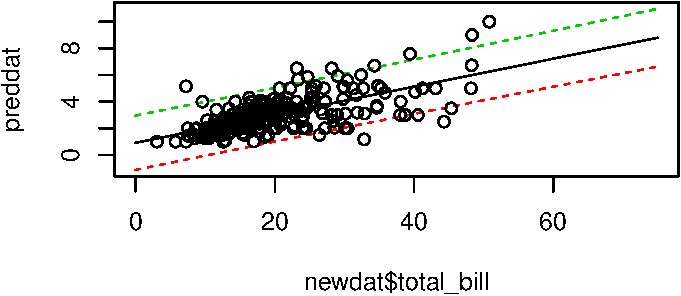
\includegraphics{DatenerhebungStatistik-Uebung_files/figure-latex/unnamed-chunk-187-1.pdf}

Sie sehen, dass 95\(\,\)\% Prognoseintervall ist recht breit: über den
gewählten Rechnungsbereich von \(0-75\)\(\,\)\$ im Mittelwert bei
4.11\(\,\)\$.

\begin{Shaded}
\begin{Highlighting}[]
\KeywordTok{favstats}\NormalTok{((preddat[,}\DecValTok{3}\NormalTok{]}\OperatorTok{-}\NormalTok{preddat[,}\DecValTok{2}\NormalTok{]))}
\end{Highlighting}
\end{Shaded}

\begin{verbatim}
##       min       Q1   median       Q3      max     mean         sd  n
##  4.034738 4.044428 4.072224 4.171158 4.341141 4.115859 0.09042352 76
##  missing
##        0
\end{verbatim}

Zu den Rändern hin wird es breiter. Am schmalsten ist es übrigens beim
Mittelwert der unabhängigen Beobachtungen, hier also bei 19.79\(\,\)\$.

\hypertarget{kreuzvalidierung}{%
\subsection{Kreuzvalidierung}\label{kreuzvalidierung}}

Je komplexer und flexibler ein Modell ist, desto besser kann es sich an
die \emph{vorhandenen}, sogenannte Traininingsdaten anpassen,
\textbf{aber} für \emph{neue}, sogenannte Testdaten wird es nicht immer
besser -- siehe z. B. Kapitel 2.2 aus
\href{http://www-bcf.usc.edu/~gareth/ISL/}{James et. al (2013)}.

Allgemein können Modelle mit Hilfe des Mean Squared Error verglichen
werden: \[ MSE = \frac{1}{n} \sum_{i=1}^n (y_i - \hat{f}(x_i))^2\]
Vorhandene Daten können aber genutzt werden um die Prognose für neue
Daten \((x_0,y_0)\) zu simulieren: z. B. über Kreuzvalidierung. Im
einfachen Fall einer Leave-One-Out Kreuzvalidierung werden alle
Beobachtungen bis auf die \(i\text{-}te, \quad i=1,2,\ldots n\) zum
Schätzen oder Lernen des Modells verwendet, das Testen des Modells
erfolgt dann anhand der Prognosegüte für die
\(i\text{-}te, \quad i=1,2,\ldots n\) Beobachtung. In R kann dies
einfach über \emph{Schleifen} durchgeführt werden:

\begin{Shaded}
\begin{Highlighting}[]
\NormalTok{n <-}\StringTok{ }\KeywordTok{nrow}\NormalTok{(tips) }\CommentTok{# Anzahl Beobachtungen}
\NormalTok{y <-}\StringTok{ }\NormalTok{tips}\OperatorTok{$}\NormalTok{tip }\CommentTok{# "Wahre" Werte}
\NormalTok{yprog <-}\StringTok{ }\KeywordTok{numeric}\NormalTok{(n) }\CommentTok{# Vektor in dem die Prognosen geschrieben werden}

\CommentTok{### Modellanpassung}
\NormalTok{mod <-}\StringTok{ }\KeywordTok{lm}\NormalTok{(tip }\OperatorTok{~}\StringTok{ }\NormalTok{., }\DataTypeTok{data=}\NormalTok{tips) }\CommentTok{# Modell mit allen Beobachtungen schätzen}
\NormalTok{yfit <-}\StringTok{ }\NormalTok{mod}\OperatorTok{$}\NormalTok{fitted.values }\CommentTok{# "Vorhersagen" für Trainingsdaten}

\CommentTok{### Leave-One-Out Kreuzvalidierung}
\ControlFlowTok{for}\NormalTok{ (i }\ControlFlowTok{in} \DecValTok{1}\OperatorTok{:}\NormalTok{n) }\CommentTok{# i nehme nacheinander die Werte von 1 bis n an}
\NormalTok{\{}
  \CommentTok{# Modell schätzen ohne i-te Beobachtung}
\NormalTok{  modloo <-}\StringTok{ }\KeywordTok{lm}\NormalTok{(tip }\OperatorTok{~}\StringTok{ }\NormalTok{., }\DataTypeTok{data=}\NormalTok{tips[}\OperatorTok{-}\NormalTok{i,]) }
  \CommentTok{# Vorhersage von y_i anhand des Modells}
\NormalTok{  yprog[i] <-}\StringTok{ }\KeywordTok{predict}\NormalTok{(modloo, }\DataTypeTok{newdata =}\NormalTok{ tips[i,]) }
\NormalTok{\}}

\CommentTok{### Vergleich:}
\NormalTok{MSEfit <-}\StringTok{ }\KeywordTok{mean}\NormalTok{((y}\OperatorTok{-}\NormalTok{yfit)}\OperatorTok{^}\DecValTok{2}\NormalTok{)}
\NormalTok{MSEprog <-}\StringTok{ }\KeywordTok{mean}\NormalTok{((y}\OperatorTok{-}\NormalTok{yprog)}\OperatorTok{^}\DecValTok{2}\NormalTok{)}

\KeywordTok{cat}\NormalTok{(}\StringTok{"MSE Modellanpassung: "}\NormalTok{, MSEfit, }\StringTok{"}\CharTok{\textbackslash{}n}\StringTok{"}\NormalTok{)}
\end{Highlighting}
\end{Shaded}

\begin{verbatim}
## MSE Modellanpassung:  1.010354
\end{verbatim}

\begin{Shaded}
\begin{Highlighting}[]
\KeywordTok{cat}\NormalTok{(}\StringTok{"MSE Kreuzvalidierung: "}\NormalTok{, MSEprog, }\StringTok{"}\CharTok{\textbackslash{}n}\StringTok{"}\NormalTok{)}
\end{Highlighting}
\end{Shaded}

\begin{verbatim}
## MSE Kreuzvalidierung:  1.100501
\end{verbatim}

Der Mean Squared Error ist also bei der Leave-One-Out Kreuzvalidierung
um 9\(\,\)\% schlechter als bei der Modellanpassung.

\begin{center}\rule{0.5\linewidth}{\linethickness}\end{center}

\hypertarget{ubung-teaching-rating-3}{%
\section{Übung: Teaching Rating}\label{ubung-teaching-rating-3}}

Dieser Datensatz analysiert u. a. den Zusammenhang zwischen Schönheit
und Evaluierungsergebnis von Dozenten:

\emph{Hamermesh, D.S., and Parker, A. (2005). Beauty in the Classroom:
Instructors' Pulchritude and Putative Pedagogical Productivity.
Economics of Education Review, 24, 369--376.}

Sie können ihn, sofern noch nicht geschehen, von
\url{https://goo.gl/6Y3KoK} als \texttt{csv} herunterladen.

Versuchen Sie, das Evaluierungsergebnis als abhängige Variable anhand
geeigneter Variablen des Datensatzes zu erklären. Wie groß ist der
Einfluss der Schönheit? Sind die Modellannahmen erfüllt und wie
beurteilen Sie die Modellgüte?

\hypertarget{literatur-5}{%
\section{Literatur}\label{literatur-5}}

\begin{itemize}
\tightlist
\item
  David M. Diez, Christopher D. Barr, Mine Çetinkaya-Rundel (2014):
  \emph{Introductory Statistics with Randomization and Simulation},
  \url{https://www.openintro.org/stat/textbook.php?stat_book=isrs},
  Kapitel 5, 6.1-6.3
\item
  Nicholas J. Horton, Randall Pruim, Daniel T. Kaplan (2015): Project
  MOSAIC Little Books \emph{A Student's Guide to R},
  \url{https://github.com/ProjectMOSAIC/LittleBooks/raw/master/StudentGuide/MOSAIC-StudentGuide.pdf},
  Kapitel 5.4, 10.2
\item
  Gareth James, Daniela Witten, Trevor Hastie, Robert Tibshirani (2013):
  \emph{An Introduction to Statistical Learning -- with Applications in
  R}, \url{http://www-bcf.usc.edu/~gareth/ISL/}, Kapitel 3
\item
  Maike Luhmann (2015): \emph{R für Einsteiger}, Kapitel 16, 17.1-17.3
\item
  Andreas Quatember (2010): \emph{Statistik ohne Angst vor Formeln},
  Kapitel 3.11
\item
  Daniel Wollschläger (2014): \emph{Grundlagen der Datenanalyse mit R},
  Kapitel 6
\end{itemize}

\hypertarget{lizenz-5}{%
\subsection{Lizenz}\label{lizenz-5}}

Diese Übung wurde von Karsten Lübke entwickelt und orientiert sich an
der Übung zum Buch
\href{https://www.openintro.org/stat/index.php?stat_book=isrs}{OpenIntro}
von Andrew Bray, Mine Çetinkaya-Rundel und steht wie diese unter der
Lizenz \href{http://creativecommons.org/licenses/by-sa/3.0}{Creative
Commons Attribution-ShareAlike 3.0 Unported}. Kleinere Ergänzungen
stammen von Norman Markgraf

\hypertarget{versionshinweise-5}{%
\subsection{Versionshinweise:}\label{versionshinweise-5}}

\begin{itemize}
\tightlist
\item
  Datum erstellt: 2019-01-24
\item
  R Version: 3.5.1
\item
  \texttt{mosaic} Version: 1.4.0
\end{itemize}

\newpage

\hypertarget{anhang-1-r-kurzreferenz}{%
\chapter{Anhang 1: R Kurzreferenz}\label{anhang-1-r-kurzreferenz}}

\hypertarget{vorbemerkungen}{%
\section{Vorbemerkungen}\label{vorbemerkungen}}

Eine Übersicht von nützlichen R Funktionen innerhalb der Datenanalyse.

Diese Kurzreferenz beschreibt ein kleinen Teil der R Funktionen, wobei
größtenteils auf das Zusatzpaket \texttt{mosaic} zurückgegriffen wird.
Sie basiert weitgehend auf der Vignette
\href{https://cran.r-project.org/web/packages/mosaic/vignettes/MinimalR.pdf}{Minimal
R} von Randall Pruim.

Weitere Hilfe und Beispiele finden Sie, wenn Sie

\begin{Shaded}
\begin{Highlighting}[]
\OperatorTok{>}\StringTok{ }\NormalTok{?plot}
\end{Highlighting}
\end{Shaded}

eingeben.

\begin{itemize}
\tightlist
\item
  R unterscheidet zwischen Groß- und Kleinbuchstaben.
\item
  R verwendet den Punkt \texttt{.} als Dezimaltrennzeichen.
\item
  Fehlende Werte werden in R durch \texttt{NA} kodiert.
\item
  Kommentare werden mit dem Rautezeichen \texttt{\#} eingeleitet; der
  Rest der Zeile von von R dann ignoriert.
\item
  R wendet Befehle direkt an.
\item
  R ist objektorientiert, d.~h., dieselbe Funktion hat evtl. je nach
  Funktionsargument unterschiedliche Rückgabewerte.
\item
  Zusätzliche Funktionalität kann über Zusatzpakete hinzugeladen werden.
  Diese müssen ggf. zunächst installiert werden.
\item
  Mit der Pfeiltaste nach oben können Sie einen vorherigen Befehl in der
  Konsole wieder aufrufen.
\item
  Eine Ergebniszuweisung erfolgt über \texttt{\textless{}-}
\end{itemize}

Innerhalb von \texttt{mosaic}:

\begin{Shaded}
\begin{Highlighting}[]
\KeywordTok{analysiere}\NormalTok{(y }\OperatorTok{~}\StringTok{ }\NormalTok{x }\OperatorTok{|}\StringTok{ }\NormalTok{z , }\DataTypeTok{data=}\NormalTok{Daten)}
\end{Highlighting}
\end{Shaded}

d. h., modelliere \texttt{y} in Abhängigkeit von \texttt{x} getrennt
bzw. bedingt für \texttt{z} aus dem Datensatz \texttt{Daten}. Dabei
können Teile (z. B. \texttt{y} und/ oder \texttt{z}) fehlen.\footnote{Beim
  Mac ist \texttt{\textasciitilde{}} die Tastenkombination
  \texttt{alt}+\texttt{n}, \texttt{\textbar{}} die Tastenkombination
  \texttt{alt}+\texttt{7}}

Zusatzpakete müssen vor der ersten Benutzung einmalig installiert und
nach jedem Neustart von R geladen werden:

\begin{Shaded}
\begin{Highlighting}[]
\KeywordTok{install.packages}\NormalTok{(}\StringTok{"Paket"}\NormalTok{) }\CommentTok{# Einmalig installieren}
\KeywordTok{library}\NormalTok{(Paket) }\CommentTok{# Laden, einmalig in jeder Sitzung}
\end{Highlighting}
\end{Shaded}

\hypertarget{daten}{%
\section{Daten}\label{daten}}

Daten einlesen und Datenvorverarbeitung sind häufig der (zeitlich)
aufwendigste Teil einer Datenanalyse. Da die Daten die Grundlage sind,
sollte auch hier sorgfältig gearbeitet und überprüft werden.

\hypertarget{daten-einlesen}{%
\subsection{Daten einlesen}\label{daten-einlesen}}

\begin{Shaded}
\begin{Highlighting}[]
\KeywordTok{read.table}\NormalTok{() }\CommentTok{# Allgemeinen Datensatz einlesen. Achtung: Optionen anpassen}
\KeywordTok{read.csv2}\NormalTok{() }\CommentTok{# csv Datensatz einlesen (aus deutschsprachigem Excel)}
\KeywordTok{file.choose}\NormalTok{() }\CommentTok{# Datei auswählen}
\NormalTok{meineDaten <-}\StringTok{ }\KeywordTok{read.csv2}\NormalTok{(}\KeywordTok{file.choose}\NormalTok{())}
\end{Highlighting}
\end{Shaded}

U. a. mit Hilfe des Zusatzpaketes \texttt{readxl} können Excel Dateien
eingelesen werden:

\begin{Shaded}
\begin{Highlighting}[]
\NormalTok{meineDaten <-}\StringTok{ }\KeywordTok{read_excel}\NormalTok{(}\KeywordTok{file.choose}\NormalTok{()) }
\end{Highlighting}
\end{Shaded}

\hypertarget{daten-verarbeiten}{%
\subsection{Daten verarbeiten}\label{daten-verarbeiten}}

\begin{Shaded}
\begin{Highlighting}[]
\KeywordTok{str}\NormalTok{() }\CommentTok{# Datenstruktur}
\KeywordTok{head}\NormalTok{() }\CommentTok{# Obere Zeilen}
\KeywordTok{tail}\NormalTok{() }\CommentTok{# Untere Zeilen}
\KeywordTok{nrow}\NormalTok{(); }\KeywordTok{ncol}\NormalTok{() }\CommentTok{# Anzahl Zeilen; Spalten }
\KeywordTok{rownames}\NormalTok{(); }\KeywordTok{colnames}\NormalTok{() }\CommentTok{# Zeilennamen, Spaltennamen}
\end{Highlighting}
\end{Shaded}

\hypertarget{daten-transformieren}{%
\subsection{Daten transformieren}\label{daten-transformieren}}

Einzelne Variablen eines Datensatzes können über \texttt{\$} ausgewählt
werden: \texttt{Daten\$Variable}. Allgemein kann über
\texttt{Daten{[}i,j{]}} die i-te Zeile und j-te Spalte ausgewählt
werden, wobei auch mehrere oder keine Zeile(n) bzw. Spalte(n) ausgewählt
werden können. Über \texttt{c()} wird ein Vektor erzeugt. Mit \texttt{-}
vor der Auswahl werden der Rest ohne die Auswahl ausgewählt.

\begin{Shaded}
\begin{Highlighting}[]
\KeywordTok{as.factor}\NormalTok{() }\CommentTok{# Daten als Faktoren definieren}
\KeywordTok{relevel}\NormalTok{() }\CommentTok{# Faktorstufen umordnen}
\KeywordTok{droplevels}\NormalTok{() }\CommentTok{# Ungenutzte Faktorstufen entfernen}
\KeywordTok{recode}\NormalTok{() }\CommentTok{# Umkodierung von Werten, Paket car}
\KeywordTok{as.numeric}\NormalTok{() }\CommentTok{# Faktorstufen als numerische Daten verwenden}
\KeywordTok{cut}\NormalTok{() }\CommentTok{# Aufteilung numerischer Werte in Intervalle}

\KeywordTok{subset}\NormalTok{() }\CommentTok{# Teilmenge der Daten auswählen}
\KeywordTok{na.omit}\NormalTok{() }\CommentTok{# Zeilen mit fehlenden Werten entfernen}

\KeywordTok{log}\NormalTok{() }\CommentTok{# Logarithmusfunktion}
\KeywordTok{exp}\NormalTok{() }\CommentTok{# Exponentialfunktion}
\KeywordTok{sqrt}\NormalTok{() }\CommentTok{# Quadratwurzelfunktion}
\KeywordTok{abs}\NormalTok{() }\CommentTok{# Betragsfunktion}

\KeywordTok{rowSums}\NormalTok{() }\CommentTok{# Zeilensumme}
\KeywordTok{rowMeans}\NormalTok{() }\CommentTok{# Zeilenmittelwert}
\end{Highlighting}
\end{Shaded}

Innerhalb des Paketes \texttt{dplyr} (wird mit \texttt{mosaic} geladen)
gibt es u. a. folgende Funktionen:

\begin{Shaded}
\begin{Highlighting}[]
\KeywordTok{filter}\NormalTok{() }\CommentTok{# Filtert Beobachtungen eines Datensatzes}
\KeywordTok{select}\NormalTok{() }\CommentTok{# Wählt Variablen eines Datensatzes aus}
\KeywordTok{mutate}\NormalTok{() }\CommentTok{# Erzeugt neue Variable bzw. verändert bestehende}
\KeywordTok{rename}\NormalTok{() }\CommentTok{# Benennt Variablen um}
\KeywordTok{arrange}\NormalTok{() }\CommentTok{# Sortiert Beobachtungen eines Datensatzes}
\OperatorTok\StringTok{ }\CommentTok{# Übergebe das Ergebnis der vorhergehenden Funktion an die folgende}
\end{Highlighting}
\end{Shaded}

\hypertarget{grafische-verfahren}{%
\section{Grafische Verfahren}\label{grafische-verfahren}}

Vor jeder mathematisch-statistischen Analyse sollte eine explorative,
grafische Analyse erfolgen. Die folgenden Befehle sind aus dem Paket
\texttt{mosaic}.

\begin{Shaded}
\begin{Highlighting}[]
\KeywordTok{bargraph}\NormalTok{() }\CommentTok{# Balkendiagramm}
\KeywordTok{histogram}\NormalTok{() }\CommentTok{# Histogramm}
\KeywordTok{bwplot}\NormalTok{() }\CommentTok{# Boxplot}
\KeywordTok{xyplot}\NormalTok{() }\CommentTok{# Streudiagrmm}
\end{Highlighting}
\end{Shaded}

Nicht aus dem Paket \texttt{mosaic} sind:

\begin{Shaded}
\begin{Highlighting}[]
\KeywordTok{mosaicplot}\NormalTok{() }\CommentTok{# Mosaicplot}
\KeywordTok{corrplot}\NormalTok{() }\CommentTok{# Korrelationsplot, Paket corrplot}
\KeywordTok{ggpairs}\NormalTok{() }\CommentTok{# Matrixplot, Paket GGally}
\KeywordTok{heatmap}\NormalTok{() }\CommentTok{# Heatmap}
\end{Highlighting}
\end{Shaded}

\pagebreak

\hypertarget{deskriptive-statistik}{%
\section{Deskriptive Statistik}\label{deskriptive-statistik}}

Eine gute Zusammenfassung liefert der \texttt{mosaic} Befehl:

\begin{Shaded}
\begin{Highlighting}[]
\KeywordTok{favstats}\NormalTok{()}
\end{Highlighting}
\end{Shaded}

Ansonsten (\texttt{mosaic} angepasst):

\begin{Shaded}
\begin{Highlighting}[]
\KeywordTok{tally}\NormalTok{() }\CommentTok{# Tabellierung, Häufigkeiten }
\KeywordTok{prop}\NormalTok{() }\CommentTok{# Anteile}
\KeywordTok{mean}\NormalTok{() }\CommentTok{# Arithmetischer Mittelwert}
\KeywordTok{median}\NormalTok{() }\CommentTok{# Median}
\KeywordTok{quantile}\NormalTok{() }\CommentTok{# Quantile}
\KeywordTok{sd}\NormalTok{() }\CommentTok{# Standardabweichung}
\KeywordTok{var}\NormalTok{() }\CommentTok{# Varianz}
\KeywordTok{IQR}\NormalTok{() }\CommentTok{# Interquartilsabstand}
\KeywordTok{cov}\NormalTok{() }\CommentTok{# Kovarianz}
\KeywordTok{cor}\NormalTok{() }\CommentTok{# Korrelationskoefizient}
\end{Highlighting}
\end{Shaded}

\hypertarget{inferenzstatistik}{%
\section{Inferenzstatistik}\label{inferenzstatistik}}

\hypertarget{randomisierung-simulationen}{%
\subsection{Randomisierung,
Simulationen}\label{randomisierung-simulationen}}

Größtenteils \texttt{mosaic}:

\begin{Shaded}
\begin{Highlighting}[]
\KeywordTok{set.seed}\NormalTok{() }\CommentTok{# Zufallszahlengenerator setzen}
\KeywordTok{rflip}\NormalTok{() }\CommentTok{# Münzwurf}
\KeywordTok{do}\NormalTok{() }\CommentTok{# Wiederholung (Schleife)}
\KeywordTok{sample}\NormalTok{() }\CommentTok{# Stichprobe ohne Zurücklegen}
\KeywordTok{resample}\NormalTok{() }\CommentTok{# Stichprobe mit Zurücklegen}
\KeywordTok{shuffle}\NormalTok{() }\CommentTok{# Permutation}
\KeywordTok{rnorm}\NormalTok{() }\CommentTok{# Normalverteilte Zufallszahlen}
\end{Highlighting}
\end{Shaded}

\hypertarget{verteilungen}{%
\subsection{Verteilungen}\label{verteilungen}}

Innerhalb der Funktionen müssen ggf. die Parameter, d.~h.
\texttt{mean=}, \texttt{sd=} bzw. \texttt{df=} angepasst werden. (Das
vorgestellte \texttt{x} steht für in \texttt{mosaic} angepasste
Versionen.)

\begin{Shaded}
\begin{Highlighting}[]
\KeywordTok{xpchisq}\NormalTok{() }\CommentTok{# Verteilungsfunktion Chi² Verteilung}
\KeywordTok{xqchisq}\NormalTok{() }\CommentTok{# Quantilsfunktion Chi² Verteilung}
\KeywordTok{xpnorm}\NormalTok{() }\CommentTok{# Verteilungsfunktion Normalverteilung}
\KeywordTok{xqnorm}\NormalTok{() }\CommentTok{# Quantilsfunktion Normalverteilung}
\KeywordTok{xpt}\NormalTok{() }\CommentTok{# Verteilungsfunktion t-Vverteilung}
\KeywordTok{xqt}\NormalTok{() }\CommentTok{# Quantilsfunktion t-Vverteilung}
\end{Highlighting}
\end{Shaded}

Analoger Aufbau für weitere Verteilungen, z. B. \texttt{\_binom()}
(Binomialverteilung), \texttt{\_f()} (F\_Verteilung).

\hypertarget{testverfahren}{%
\subsection{Testverfahren}\label{testverfahren}}

Einige der Testverfahren wurden von \texttt{mosaic} angepasst.

\begin{Shaded}
\begin{Highlighting}[]
\KeywordTok{t.test}\NormalTok{() }\CommentTok{# t-Test}
\KeywordTok{prop.test}\NormalTok{() }\CommentTok{# Binomialtest (approximativ)}
\KeywordTok{xchisq.test}\NormalTok{() }\CommentTok{# Chi²-Test}
\KeywordTok{aov}\NormalTok{() }\CommentTok{# Varianzanalyse}
\end{Highlighting}
\end{Shaded}

Der nicht-parametrische Wilcoxon-Test \texttt{wilcox.test()} ist nicht
im Paket \texttt{mosaic} enthalten, hat daher einen leicht anderen
Funktionsaufruf. Einen Test auf Normalverteilung führt der Shapiro-Wilk
Test durch: \texttt{shapiro.test()}.

\hypertarget{multivariate-verfahren}{%
\section{Multivariate Verfahren}\label{multivariate-verfahren}}

\begin{Shaded}
\begin{Highlighting}[]
\KeywordTok{lm}\NormalTok{() }\CommentTok{# Lineare Regression}
\KeywordTok{glm}\NormalTok{(, }\DataTypeTok{family=}\StringTok{"binomial"}\NormalTok{) }\CommentTok{# Logistische Regression}
\KeywordTok{plotModel}\NormalTok{() }\CommentTok{# Modell zeichnen}
\KeywordTok{coef}\NormalTok{() }\CommentTok{# Koeffizienten extrahieren}
\KeywordTok{residuals}\NormalTok{() }\CommentTok{# Residuen einer Regression}
\KeywordTok{fitted}\NormalTok{() }\CommentTok{# Angepasste Werte einer Regression}
\KeywordTok{predict}\NormalTok{() }\CommentTok{# Vorhersagen}
\end{Highlighting}
\end{Shaded}

In \texttt{mosaic} kann das Ergebnis einer solchen Regression über
\texttt{makeFun()} in eine einfache mathematische Funktion überführt
werden. \texttt{plotFun()} zeichnet das Ergebnis. \texttt{step()} führt
eine Variablenselektion durch.

Weitere Verfahren -- nicht \texttt{mosaic}:

\begin{Shaded}
\begin{Highlighting}[]
\KeywordTok{prcomp}\NormalTok{() }\CommentTok{# Hauptkomponentenanalyse (PCA)}
\KeywordTok{alpha}\NormalTok{() }\CommentTok{# Reliabilitätsanalys, Paket psych}
\KeywordTok{dist}\NormalTok{() }\CommentTok{# Distanzen}
\KeywordTok{hclust}\NormalTok{() }\CommentTok{# Hierachische Clusteranalyse}
\KeywordTok{kmeans}\NormalTok{() }\CommentTok{# k-Means Clusterverfahren}
\KeywordTok{rpart}\NormalTok{() }\CommentTok{# Klassifikations- und Regressionsbäume, Paket rpart}
\end{Highlighting}
\end{Shaded}

\hypertarget{versionshinweise-6}{%
\subsection{Versionshinweise:}\label{versionshinweise-6}}

Erstellt von Karsten Lübke unter der Lizenz
\href{http://creativecommons.org/licenses/by-sa/3.0}{Creative Commons
Attribution-ShareAlike 3.0 Unported}.

\begin{itemize}
\tightlist
\item
  Datum erstellt: 2019-01-24
\item
  R Version: 3.5.1
\item
  \texttt{mosaic} Version: 1.4.0
\end{itemize}

\hypertarget{anhang-2-datenjudo}{%
\chapter{Anhang 2: Datenjudo}\label{anhang-2-datenjudo}}

\begin{figure}

{\centering 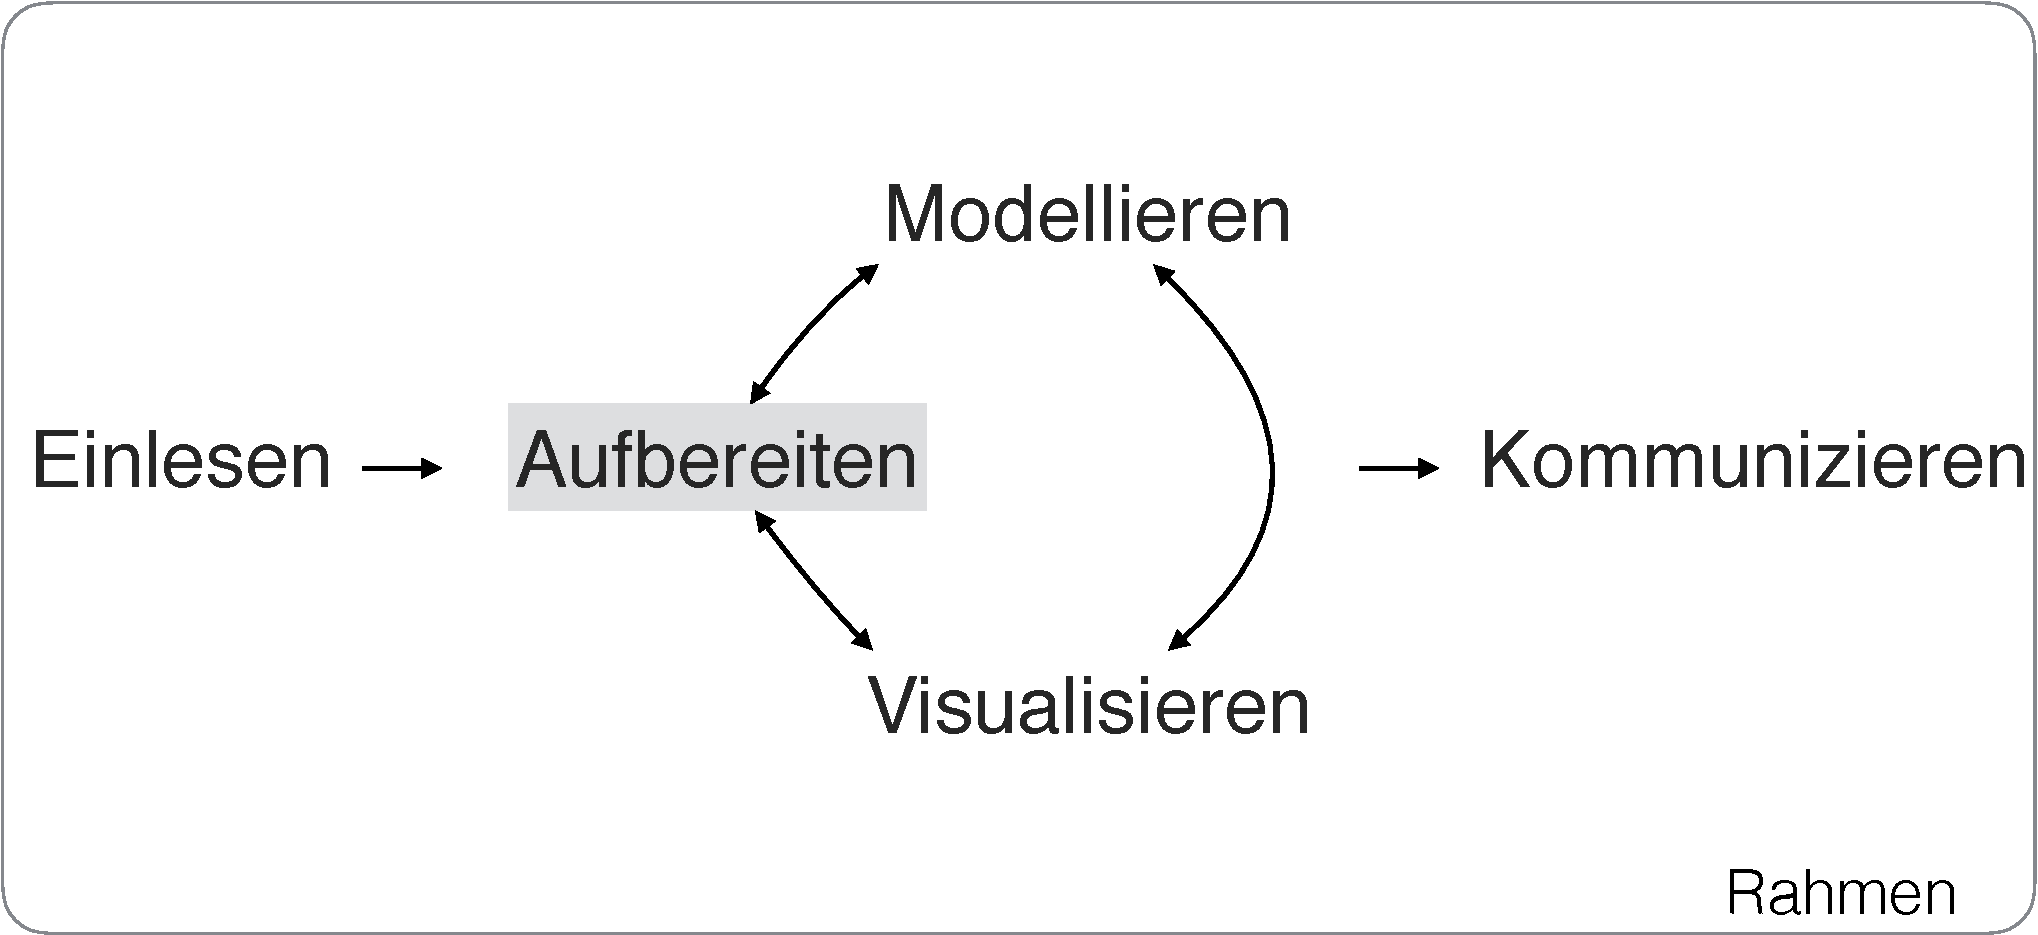
\includegraphics{Inhalte/images/Datenjudo/Aufbereiten} 

}

\caption{Daten aufbereiten}\label{fig:unnamed-chunk-207}
\end{figure}

In diesem Kapitel benötigte Pakete:

\begin{Shaded}
\begin{Highlighting}[]
\CommentTok{# library(tidyverse)}
\CommentTok{# Hinweis: tidyverse durch die einzelnen tidy core Pakete ersetzt, da (noch) nicht alle Pakete von tidyverse, die sonst noch mitgeladen werden, unter R 3.5 verfügbar sind}
\KeywordTok{library}\NormalTok{(ggplot2) }\CommentTok{# Datenjudo}
\KeywordTok{library}\NormalTok{(dplyr)}
\KeywordTok{library}\NormalTok{(tidyr)}
\KeywordTok{library}\NormalTok{(readr)}
\KeywordTok{library}\NormalTok{(purrr)}
\KeywordTok{library}\NormalTok{(tibble)}
\end{Highlighting}
\end{Shaded}

\begin{verbatim}
## Warning: package 'tibble' was built under R version 3.5.2
\end{verbatim}

\begin{Shaded}
\begin{Highlighting}[]
\KeywordTok{library}\NormalTok{(stringr)}
\KeywordTok{library}\NormalTok{(forcats) }\CommentTok{# Ende Einzelpakete}
\KeywordTok{library}\NormalTok{(car)  }\CommentTok{# für 'recode'}
\end{Highlighting}
\end{Shaded}

Mit \emph{Datenjudo} ist gemeint, die Daten für die eigentliche Analyse
\enquote{aufzubereiten}. Unter \emph{Aufbereiten} ist hier das Umformen,
Prüfen, Bereinigen, Gruppieren und Zusammenfassen von Daten gemeint. Die
deskriptive Statistik fällt unter die Rubrik Aufbereiten. Kurz gesagt:
Alles, was man tut, nachdem die Daten \enquote{da} sind und bevor man
mit anspruchsvoller(er) Modellierung beginnt.

Ist das Aufbereiten von Daten auch nicht statistisch anspruchsvoll, so
ist es trotzdem von großer Bedeutung und häufig recht zeitintensiv. Eine
Anekdote zur Relevanz der Datenaufbereitung, die (so will es die
Geschichte) mir an einer Bar nach einer einschlägigen Konferenz erzählt
wurde (daher keine Quellenangebe, Sie verstehen\ldots{}). Eine
Computerwissenschaftlerin aus den USA (deutschen Ursprungs) hatte einen
beeindruckenden \enquote{Track Record} an Siegen in Wettkämpfen der
Datenanalyse. Tatsächlich hatte sie keine besonderen, raffinierten
Modellierungstechniken eingesetzt; klassische Regression war ihre
Methode der Wahl. Bei einem Wettkampf, bei dem es darum ging, Krebsfälle
aus Krankendaten vorherzusagen (z. B. von Röntgenbildern) fand sie nach
langem Datenjudo heraus, dass in die \enquote{ID-Variablen} Information
gesickert war, die dort nicht hingehörte und die sie nutzen konnte für
überraschend (aus Sicht der Mitstreiter) gute Vorhersagen zu
Krebsfällen. Wie war das möglich? Die Daten stammten aus mehreren
Kliniken, jede Klinik verwendete ein anderes System, um IDs für
Patienten zu erstellen. Überall waren die IDs stark genug, um die
Anonymität der Patienten sicherzustellen, aber gleich wohl konnte man
(nach einigem Judo) unterscheiden, welche ID von welcher Klinik stammte.
Was das bringt? Einige Kliniken waren reine Screening-Zentren, die die
Normalbevölkerung versorgte. Dort sind wenig Krebsfälle zu erwarten.
Andere Kliniken jedoch waren Onkologie-Zentren für bereits bekannte
Patienten oder für Patienten mit besonderer Risikolage. Wenig
überraschend, dass man dann höhere Krebsraten vorhersagen kann.
Eigentlich ganz einfach; besondere Mathe steht hier (zumindest in dieser
Geschichte) nicht dahinter. Und, wenn man den Trick kennt, ganz einfach.
Aber wie so oft ist es nicht leicht, den Trick zu finden. Sorgfältiges
Datenjudo hat hier den Schlüssel zum Erfolg gebracht.

\hypertarget{typische-probleme}{%
\section{Typische Probleme}\label{typische-probleme}}

Bevor man seine Statistik-Trickkiste so richtig schön aufmachen kann,
muss man die Daten häufig erst noch in Form bringen. Das ist nicht
schwierig in dem Sinne, dass es um komplizierte Mathe ginge. Allerdings
braucht es mitunter recht viel Zeit und ein paar (oder viele)
handwerkliche Tricks sind hilfreich. Hier soll das folgende Kapitel
helfen.

Typische Probleme, die immer wieder auftreten, sind:

\begin{itemize}
\tightlist
\item
  \emph{Fehlende Werte}: Irgend jemand hat auf eine meiner schönen
  Fragen in der Umfrage nicht geantwortet!
\item
  \emph{Unerwartete Daten}: Auf die Frage, wie viele Facebook-Freunde er
  oder sie habe, schrieb die Person \enquote{I like you a lot}. Was
  tun???
\item
  \emph{Daten müssen umgeformt werden}: Für jede der beiden Gruppen
  seiner Studie hat Joachim einen Google-Forms-Fragebogen aufgesetzt.
  Jetzt hat er zwei Tabellen, die er \enquote{verheiraten} möchte. Geht
  das?
\item
  \emph{Neue Variablen (Spalten) berechnen}: Ein Student fragt nach der
  Anzahl der richtigen Aufgaben in der Statistik-Probeklausur. Wir
  wollen helfen und im entsprechenden Datensatz eine Spalte erzeugen, in
  der pro Person die Anzahl der richtig beantworteten Fragen steht.
\end{itemize}

\hypertarget{daten-aufbereiten-mit-dplyr}{%
\section{\texorpdfstring{Daten aufbereiten mit
\texttt{dplyr}}{Daten aufbereiten mit dplyr}}\label{daten-aufbereiten-mit-dplyr}}

Es gibt viele Möglichkeiten, Daten mit R aufzubereiten; \texttt{dplyr}
ist ein populäres Paket dafür. Eine zentrale Idee von \texttt{dplyr}
ist, dass es nur ein paar wenige Grundbausteine geben sollte, die sich
gut kombinieren lassen. Sprich: Wenige grundlegende Funktionen mit eng
umgrenzter Funktionalität. Der Autor, Hadley Wickham, sprach einmal in
einem Forum (citation needed), dass diese Befehle wenig können, das
Wenige aber gut. Ein Nachteil dieser Konzeption kann sein, dass man
recht viele dieser Bausteine kombinieren muss, um zum gewünschten
Ergebnis zu kommen. Außerdem muss man die Logik des Baukastens gut
verstanden habe -- die Lernkurve ist also erstmal steiler. Dafür ist man
dann nicht darauf angewiesen, dass es irgendwo \enquote{Mrs Right} gibt,
die genau das kann, was ich will. Außerdem braucht man sich auch nicht
viele Funktionen merken. Es reicht, einen kleinen Satz an Funktionen zu
kennen (die praktischerweise konsistent in Syntax und Methodik sind).

Willkommen in der Welt von \texttt{dyplr}! \texttt{dplyr} hat seinen
Namen, weil es sich ausschließlich um \emph{D}ataframes bemüht; es
erwartet einen Dataframe als Eingabe und gibt einen Dataframe zurück
(zumindest bei den meisten Befehlen).

Diese Bausteine sind typische Tätigkeiten im Umgang mit Daten; nichts
Überraschendes. Schauen wir uns diese Bausteine näher an.

\hypertarget{zeilen-filtern-mit-filter}{%
\section{\texorpdfstring{Zeilen filtern mit
\texttt{filter}}{Zeilen filtern mit filter}}\label{zeilen-filtern-mit-filter}}

Häufig will man bestimmte Zeilen aus einer Tabelle filtern. Zum Beispiel
man arbeitet für die Zigarettenindustrie und ist nur an den Rauchern
interessiert (die im Übrigen unser Gesundheitssystem retten), nicht an
Nicht-Rauchern; es sollen die nur Umsatzzahlen des letzten Quartals
untersucht werden, nicht die vorherigen Quartale; es sollen nur die
Daten aus Labor X (nicht Labor Y) ausgewertet werden etc.

Ein Sinnbild:

\begin{figure}

{\centering 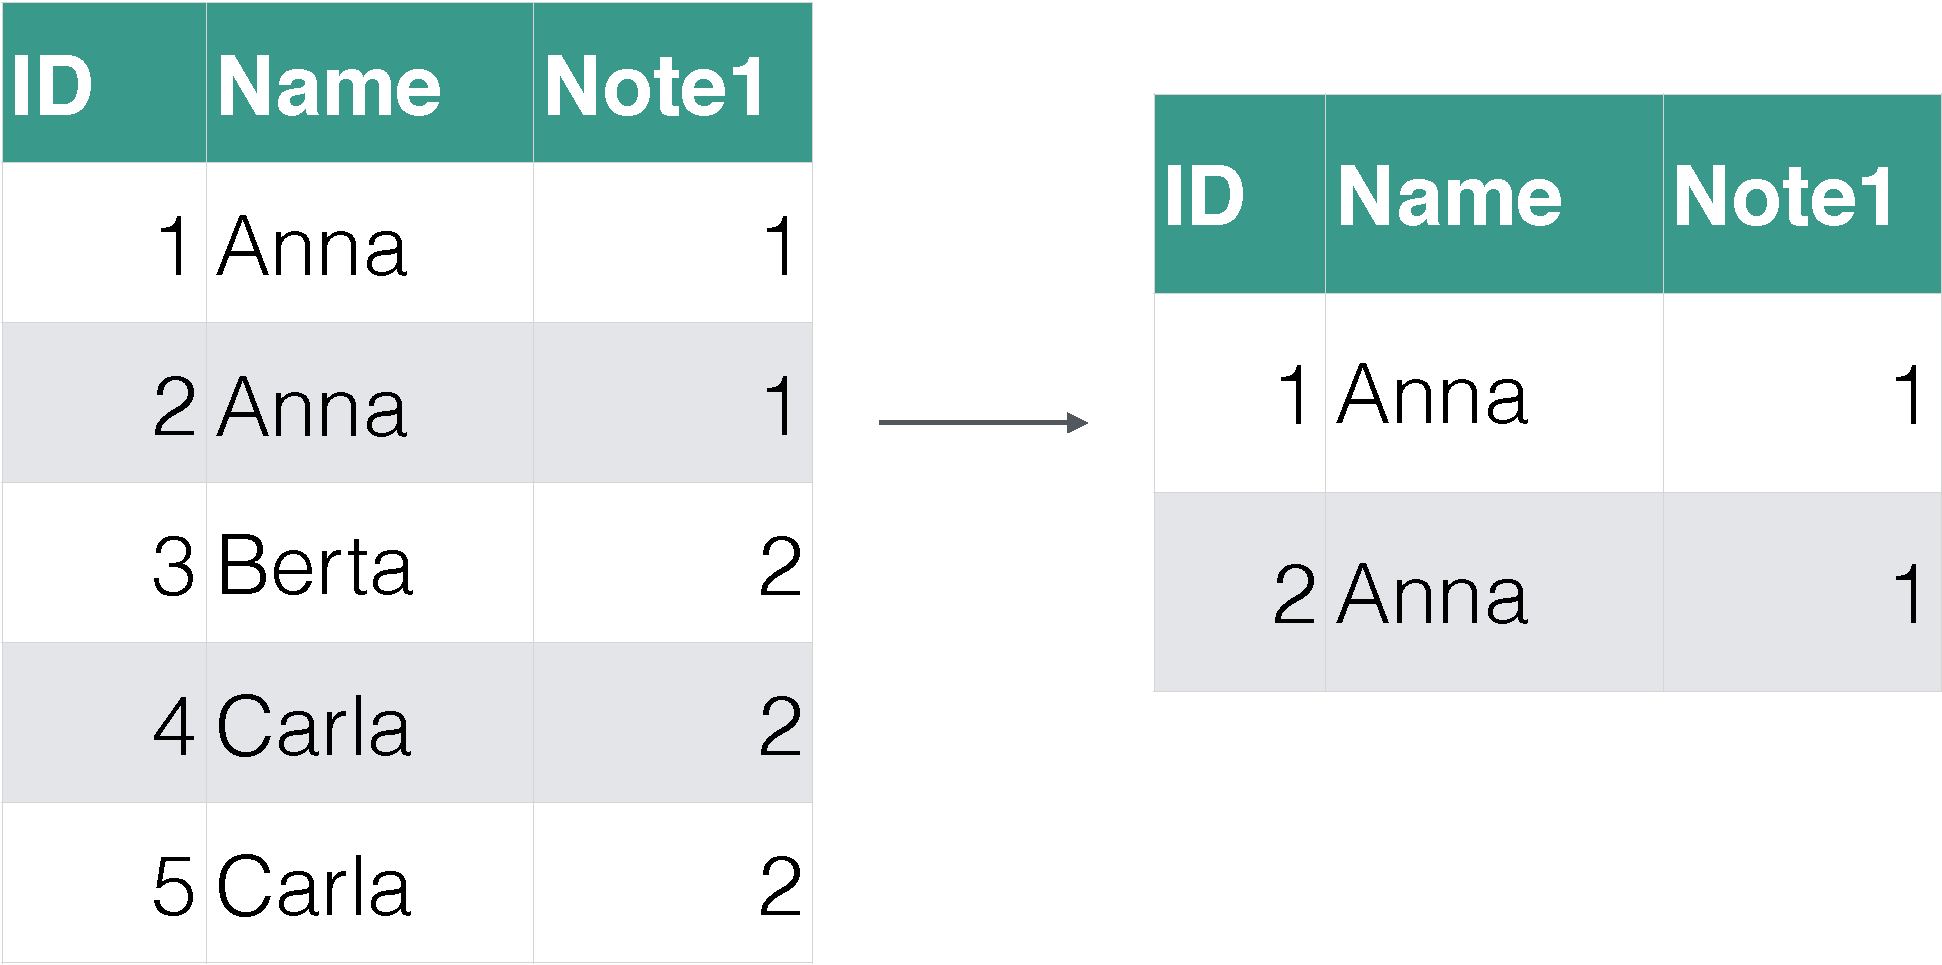
\includegraphics[width=0.6\linewidth]{Inhalte/images/Datenjudo/filter} 

}

\caption{Zeilen filtern}\label{fig:fig-filter}
\end{figure}

Merke:

\begin{quote}
Die Funktion \texttt{filter} filtert Zeilen aus einem Dataframe.
\end{quote}

Schauen wir uns einige Beispiel an; zuerst die Daten laden nicht
vergessen. Achtung: \enquote{Wohnen} die Daten in einem Paket, muss
dieses Paket installiert sein, damit man auf die Daten zugreifen kann.

\begin{Shaded}
\begin{Highlighting}[]
\KeywordTok{data}\NormalTok{(profiles, }\DataTypeTok{package =} \StringTok{"okcupiddata"}\NormalTok{)  }\CommentTok{# Das Paket muss installiert sein}
\end{Highlighting}
\end{Shaded}

\begin{Shaded}
\begin{Highlighting}[]
\NormalTok{df_frauen <-}\StringTok{ }\KeywordTok{filter}\NormalTok{(profiles, sex }\OperatorTok{==}\StringTok{ "f"}\NormalTok{)  }\CommentTok{# nur die Frauen}
\NormalTok{df_alt <-}\StringTok{ }\KeywordTok{filter}\NormalTok{(profiles, age }\OperatorTok{>}\StringTok{ }\DecValTok{70}\NormalTok{)  }\CommentTok{# nur die alten}
\CommentTok{# nur die alten Frauen, d. h. UND-Verknüpfung}
\NormalTok{df_alte_frauen <-}\StringTok{ }\KeywordTok{filter}\NormalTok{(profiles, age }\OperatorTok{>}\StringTok{ }\DecValTok{70}\NormalTok{, sex }\OperatorTok{==}\StringTok{ "f"}\NormalTok{)  }
\NormalTok{df_nosmoke_nodrinks <-}\StringTok{ }\KeywordTok{filter}\NormalTok{(profiles, smokes }\OperatorTok{==}\StringTok{ "no"} \OperatorTok{|}\StringTok{ }\NormalTok{drinks }\OperatorTok{==}\StringTok{ "not at all"}\NormalTok{) }
\CommentTok{# liefert alle Personen, die Nicht-Raucher *oder* Nicht-Trinker sind}
\end{Highlighting}
\end{Shaded}

Gar nicht so schwer, oder? Allgemeiner gesprochen werden diejenigen
Zeilen gefiltert (also behalten bzw. zurückgeliefert), für die das
Filterkriterium \texttt{TRUE} ist.

Manche Befehle wie \texttt{filter} haben einen Allerweltsnamen; gut
möglich, dass ein Befehl mit gleichem Namen in einem anderen (geladenen)
Paket existiert. Das kann dann zu Verwirrungen führen - und kryptischen
Fehlern. Im Zweifel den Namen des richtigen Pakets ergänzen, und zwar
zum Beispiel so: \texttt{dplyr::filter(...)}.

\hypertarget{aufgaben}{%
\subsection{Aufgaben}\label{aufgaben}}

Richtig oder Falsch!?\footnote{F, R, F, F, R}

\begin{enumerate}
\def\labelenumi{\arabic{enumi}.}
\tightlist
\item
  \texttt{filter} filtert Spalten.
\item
  \texttt{filter} ist eine Funktion aus dem Paket \texttt{dplyr}.
\item
  \texttt{filter} erwartet als ersten Parameter das Filterkriterium.
\item
  \texttt{filter} lässt nur ein Filterkriterium zu.
\item
  Möchte man aus dem Datensatz \texttt{profiles} (\texttt{okcupiddata})
  die Frauen filtern, so ist folgende Syntax korrekt: `filter(profiles,
  sex == \enquote{f})´.
\end{enumerate}

\hypertarget{vertiefung-fortgeschrittene-beispiele-fur-filter}{%
\section{\texorpdfstring{Vertiefung: Fortgeschrittene Beispiele für
\texttt{filter}}{Vertiefung: Fortgeschrittene Beispiele für filter}}\label{vertiefung-fortgeschrittene-beispiele-fur-filter}}

Einige fortgeschrittene Beispiele für \texttt{filter}:

Man kann alle Elemente (Zeilen) filtern, die zu einer Menge gehören und
zwar mit diesem Operator: \texttt{\%in\%}:

\begin{Shaded}
\begin{Highlighting}[]
\KeywordTok{filter}\NormalTok{(profiles, body_type }\OperatorTok\StringTok{ }\KeywordTok{c}\NormalTok{(}\StringTok{"a little extra"}\NormalTok{, }\StringTok{"average"}\NormalTok{))}
\end{Highlighting}
\end{Shaded}

Besonders Textdaten laden zu einigen Extra-Überlegungen ein; sagen wir,
wir wollen alle Personen filtern, die Katzen bei den Haustieren
erwähnen. Es soll reichen, wenn \texttt{cat} ein Teil des Textes ist;
also \texttt{likes\ dogs\ and\ likes\ cats} wäre OK (soll gefiltert
werden). Dazu nutzen wir ein Paket zur Bearbeitung von Strings
(Textdaten):

\begin{Shaded}
\begin{Highlighting}[]
\KeywordTok{filter}\NormalTok{(profiles, }\KeywordTok{str_detect}\NormalTok{(pets, }\StringTok{"cats"}\NormalTok{))}
\end{Highlighting}
\end{Shaded}

Ein häufiger Fall ist, Zeilen \emph{ohne} fehlende Werte (\texttt{NA}s)
zu filtern. Das geht einfach:

\begin{Shaded}
\begin{Highlighting}[]
\NormalTok{profiles_keine_nas <-}\StringTok{ }\KeywordTok{na.omit}\NormalTok{(profiles)}
\end{Highlighting}
\end{Shaded}

Aber was ist, wenn wir nur bei bestimmten Spalten wegen fehlender Werte
besorgt sind? Sagen wir bei \texttt{income} und bei \texttt{sex}:

\begin{Shaded}
\begin{Highlighting}[]
\KeywordTok{filter}\NormalTok{(profiles, }\OperatorTok{!}\KeywordTok{is.na}\NormalTok{(income) }\OperatorTok{|}\StringTok{ }\OperatorTok{!}\KeywordTok{is.na}\NormalTok{(sex))}
\end{Highlighting}
\end{Shaded}

\hypertarget{spalten-wahlen-mit-select}{%
\section{\texorpdfstring{Spalten wählen mit
\texttt{select}}{Spalten wählen mit select}}\label{spalten-wahlen-mit-select}}

Das Gegenstück zu \texttt{filter} ist \texttt{select}; dieser Befehl
liefert die gewählten Spalten zurück. Das ist häufig praktisch, wenn der
Datensatz sehr \enquote{breit} ist, also viele Spalten enthält. Dann
kann es übersichtlicher sein, sich nur die relevanten auszuwählen. Das
Sinnbild für diesen Befehl:

\begin{figure}

{\centering 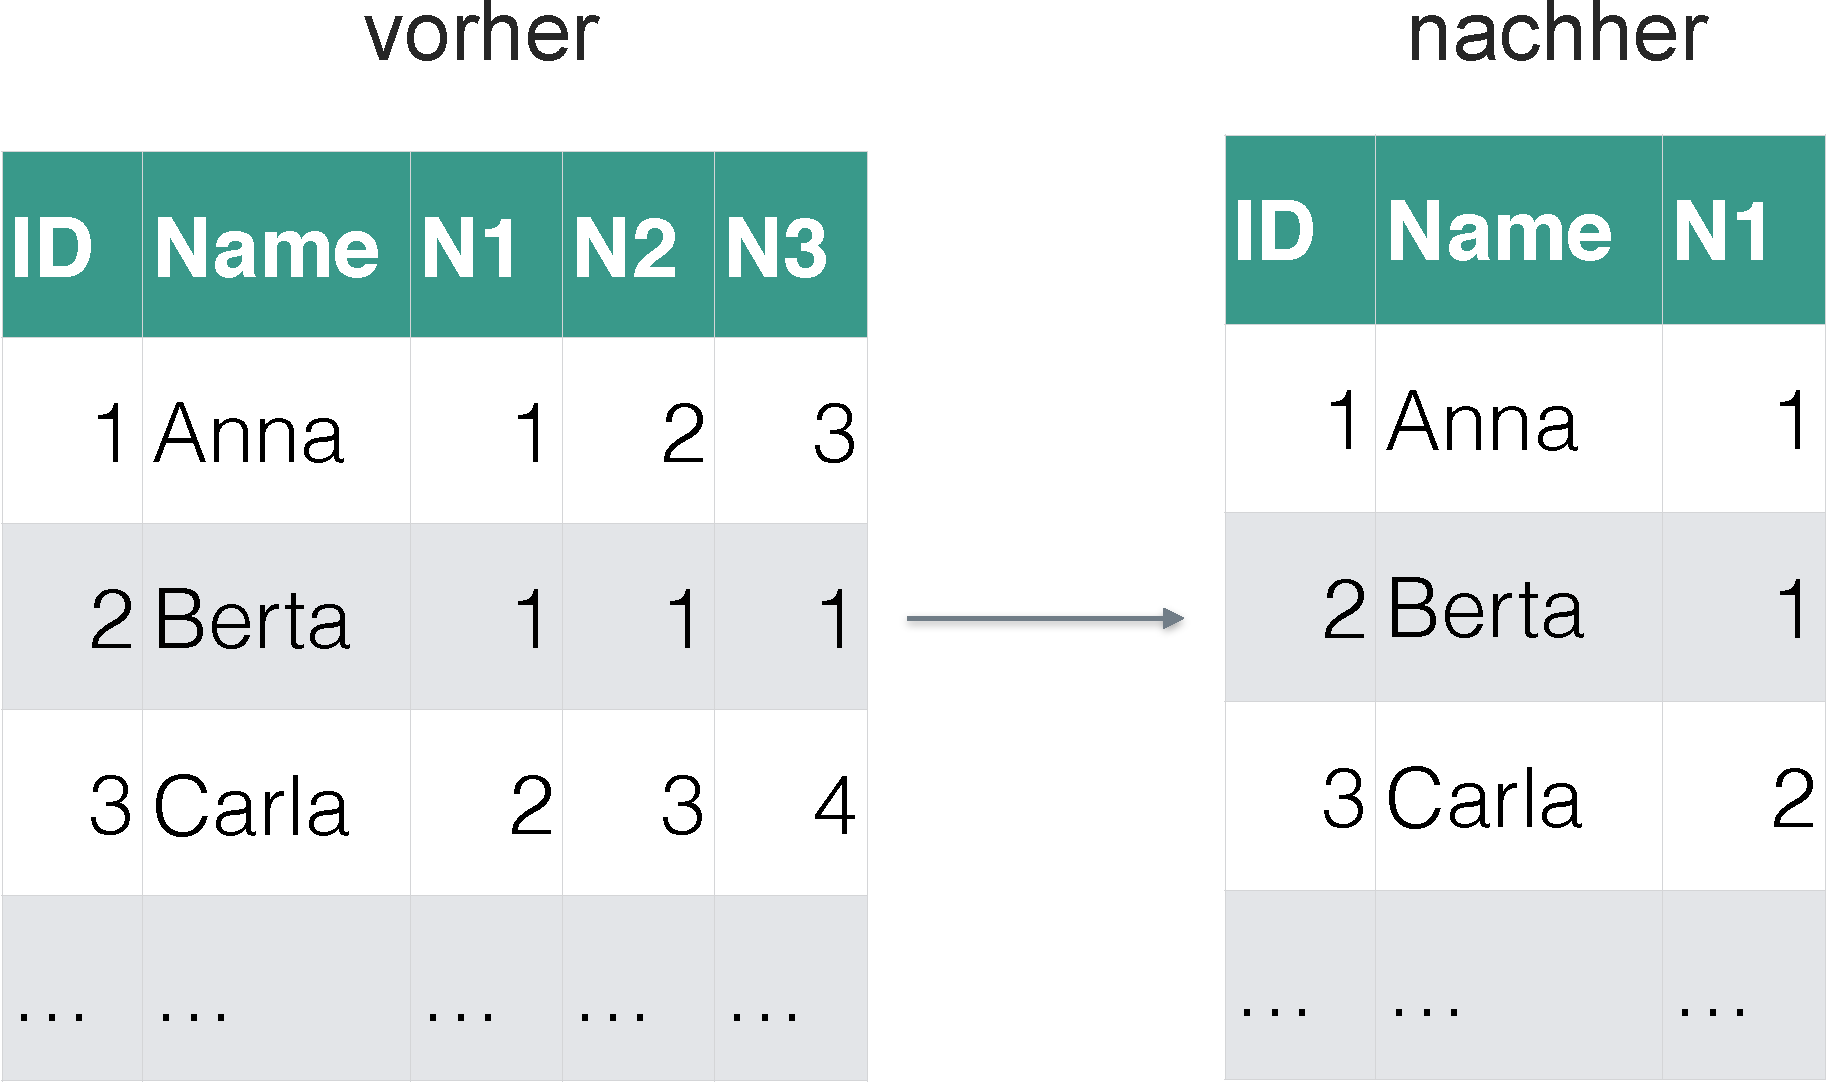
\includegraphics[width=0.6\linewidth]{Inhalte/images/Datenjudo/select} 

}

\caption{Spalten auswählen}\label{fig:fig-select}
\end{figure}

Merke:

\begin{quote}
Die Funktion \texttt{select} wählt Spalten aus einem Dataframe aus.
\end{quote}

Laden wir als ersten einen Datensatz.

\begin{Shaded}
\begin{Highlighting}[]
\NormalTok{stats_test <-}\StringTok{ }\KeywordTok{read.csv}\NormalTok{(}\StringTok{"./data/test_inf_short.csv"}\NormalTok{)}
\end{Highlighting}
\end{Shaded}

Dieser Datensatz beinhaltet Daten zu einer Statistikklausur.

Beachten Sie, dass diese Syntax davon ausgeht, dass sich die Daten in
einem Unterordner mit dem Namen \texttt{data} befinden, welcher sich im
Arbeitsverzeichnis befindet\footnote{Der angegebene Pfad ist also
  \emph{relativ} zum aktuellen Verzeichnis.}.

\begin{Shaded}
\begin{Highlighting}[]
\KeywordTok{select}\NormalTok{(stats_test, score)  }\CommentTok{# Spalte `score` auswählen}
\CommentTok{# Spalten `score` und `study_time` auswählen}
\KeywordTok{select}\NormalTok{(stats_test, score, study_time)  }
\KeywordTok{select}\NormalTok{(stats_test, score}\OperatorTok{:}\NormalTok{study_time) }\CommentTok{# dito}
\KeywordTok{select}\NormalTok{(stats_test, }\DecValTok{5}\OperatorTok{:}\DecValTok{6}\NormalTok{) }\CommentTok{# Spalten 5 bis 6 auswählen}
\end{Highlighting}
\end{Shaded}

Tatsächlich ist der Befehl \texttt{select} sehr flexibel; es gibt viele
Möglichkeiten, Spalten auszuwählen. Im
\texttt{dplyr}-\href{https://www.rstudio.com/wp.../data-wrangling-cheatsheet.pdf}{Cheatsheet}
findet sich ein guter Überblick dazu.

\hypertarget{aufgaben-1}{%
\subsection{Aufgaben}\label{aufgaben-1}}

Richtig oder Falsch!?\footnote{F, F, R, R, F}

\begin{enumerate}
\def\labelenumi{\arabic{enumi}.}
\tightlist
\item
  \texttt{select} wählt \emph{Zeilen} aus.
\item
  \texttt{select} ist eine Funktion aus dem Paket \texttt{knitr}.
\item
  Möchte man zwei Spalten auswählen, so ist folgende Syntax prinzipiell
  korrekt: \texttt{select(df,\ spalte1,\ spalte2)}.
\item
  Möchte man Spalten 1 bis 10 auswählen, so ist folgende Syntax
  prinzipiell korrekt: `select(df, spalte1:spalte10)
\item
  Mit \texttt{select} können Spalten nur bei ihrem Namen, aber nicht bei
  ihrer Nummer aufgerufen werden.
\end{enumerate}

\hypertarget{zeilen-sortieren-mit-arrange}{%
\section{\texorpdfstring{Zeilen sortieren mit
\texttt{arrange}}{Zeilen sortieren mit arrange}}\label{zeilen-sortieren-mit-arrange}}

Man kann zwei Arten des Umgangs mit R unterscheiden: Zum einen der
\enquote{interaktive Gebrauch} und zum anderen \enquote{richtiges
Programmieren}. Im interaktiven Gebrauch geht es uns darum, die Fragen
zum aktuell vorliegenden Datensatz (schnell) zu beantworten. Es geht
nicht darum, eine allgemeine Lösung zu entwickeln, die wir in die Welt
verschicken können und die dort ein bestimmtes Problem löst, ohne dass
der Entwickler (wir) dabei Hilfestellung geben muss. \enquote{Richtige}
Software, wie ein R-Paket oder Microsoft Powerpoint, muss diese
Erwartung erfüllen; \enquote{richtiges Programmieren} ist dazu vonnöten.
Natürlich sind in diesem Fall die Ansprüche an die Syntax (der
\enquote{Code}, hört sich cooler an) viel höher. In dem Fall muss man
alle Eventualitäten voraussehen und sicherstellen, dass das Programm
auch beim merkwürdigsten Nutzer brav seinen Dienst tut. Wir haben hier,
beim interaktiven Gebrauch, niedrigere Ansprüche bzw. andere Ziele.

Beim interaktiven Gebrauch von R (oder beliebigen Analyseprogrammen) ist
das Sortieren von Zeilen eine recht häufige Tätigkeit. Typisches
Beispiel wäre der Lehrer, der eine Tabelle mit Noten hat und wissen
will, welche Schüler die schlechtesten oder die besten sind in einem
bestimmten Fach. Oder bei der Prüfung der Umsätze nach Filialen möchten
wir die umsatzstärksten sowie -schwächsten Niederlassungen kennen.

Ein R-Befehl hierzu ist \texttt{arrange}; einige Beispiele zeigen die
Funktionsweise am besten:

\begin{Shaded}
\begin{Highlighting}[]
\KeywordTok{arrange}\NormalTok{(stats_test, score) }\CommentTok{# liefert die *schlechtesten* Noten zuerst zurück}
\KeywordTok{arrange}\NormalTok{(stats_test, }\OperatorTok{-}\NormalTok{score) }\CommentTok{# liefert die *besten* Noten zuerst zurück}
\KeywordTok{arrange}\NormalTok{(stats_test, interest, score)}
\end{Highlighting}
\end{Shaded}

\begin{verbatim}
##     X                 V_1 study_time self_eval interest score
## 1 234 23.01.2017 18:13:15          3         1        1    17
## 2   4 06.01.2017 09:58:05          2         3        2    18
## 3 131 19.01.2017 18:03:45          2         3        4    18
## 4 142 19.01.2017 19:02:12          3         4        1    18
## 5  35 12.01.2017 19:04:43          1         2        3    19
## 6  71 15.01.2017 15:03:29          3         3        3    20
\end{verbatim}

\begin{verbatim}
##    X                 V_1 study_time self_eval interest score
## 1  3 05.01.2017 23:33:47          5        10        6    40
## 2  7 06.01.2017 14:25:49         NA        NA       NA    40
## 3 29 12.01.2017 09:48:16          4        10        3    40
## 4 41 13.01.2017 12:07:29          4        10        3    40
## 5 58 14.01.2017 15:43:01          3         8        2    40
## 6 83 16.01.2017 10:16:52         NA        NA       NA    40
\end{verbatim}

\begin{verbatim}
##     X                 V_1 study_time self_eval interest score
## 1 234 23.01.2017 18:13:15          3         1        1    17
## 2 142 19.01.2017 19:02:12          3         4        1    18
## 3 221 23.01.2017 11:40:30          1         1        1    23
## 4 230 23.01.2017 16:27:49          1         1        1    23
## 5  92 17.01.2017 17:18:55          1         1        1    24
## 6 107 18.01.2017 16:01:36          3         2        1    24
\end{verbatim}

Einige Anmerkungen: Die generelle Syntax lautet
\texttt{arrange(df,\ Spalte1,\ ...)}, wobei \texttt{df} den Dataframe
bezeichnet und \texttt{Spalte1} die erste zu sortierende Spalte; die
Punkte \texttt{...} geben an, dass man weitere Parameter übergeben kann.
Man kann sowohl numerische Spalten als auch Textspalten sortieren. Am
wichtigsten ist hier, dass man weitere Spalten übergeben kann. Dazu
gleich mehr.

Standardmäßig sortiert \texttt{arrange} \emph{aufsteigend} (weil kleine
Zahlen im Zahlenstrahl vor den großen Zahlen kommen). Möchte man diese
Reihenfolge umdrehen (große Werte zuert, d.~h. \emph{absteigend}), so
kann man ein Minuszeichen vor den Namen der Spalte setzen.

Gibt man \emph{zwei oder mehr} Spalten an, so werden pro Wert von
\texttt{Spalte1} die Werte von \texttt{Spalte2} sortiert etc; man
betrachte den Output des Beispiels oben dazu.

Merke:

\begin{quote}
Die Funktion \texttt{arrange} sortiert die Zeilen eines Datafames.
\end{quote}

Ein Sinnbild zur Verdeutlichung:

\begin{figure}

{\centering 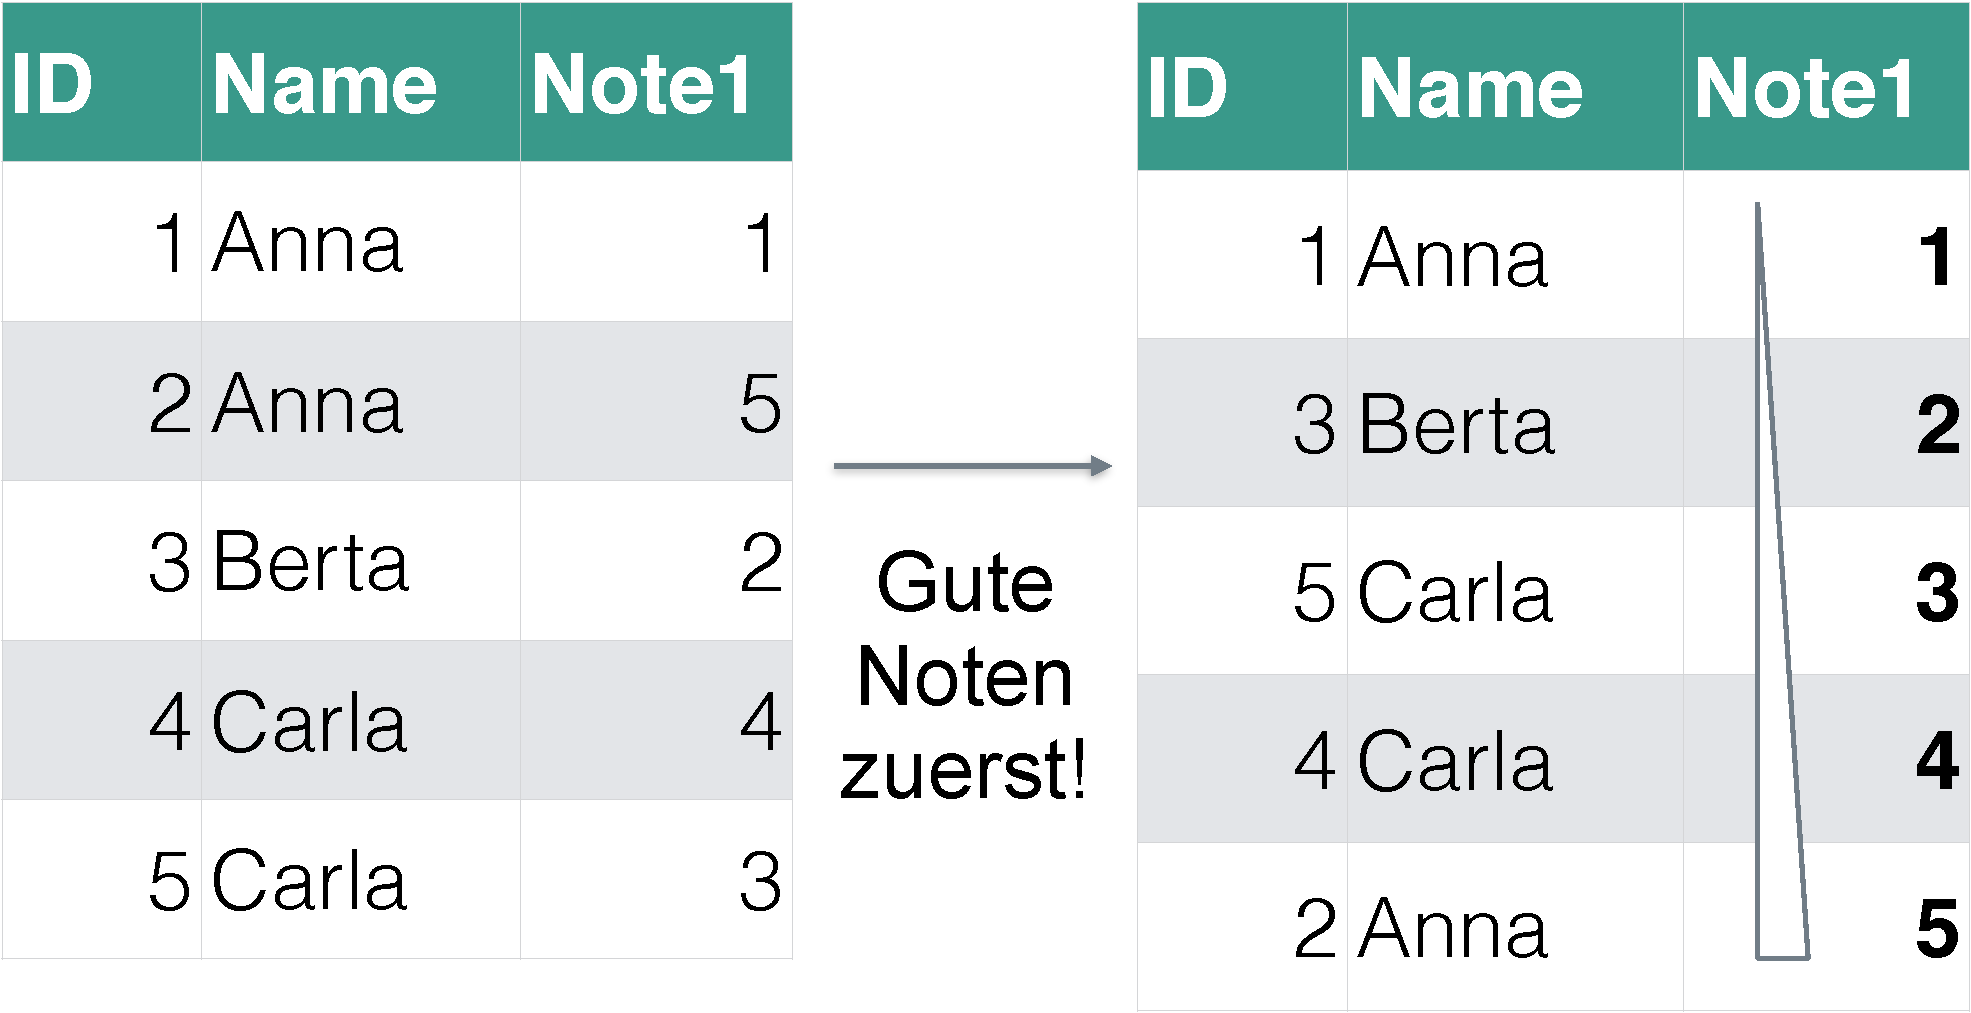
\includegraphics[width=0.6\linewidth]{Inhalte/images/Datenjudo/arrange} 

}

\caption{Spalten sortieren}\label{fig:fig-arrange}
\end{figure}

Ein ähnliches Ergebnis erhält mit man \texttt{top\_n()}, welches die
\texttt{n} \emph{größten Ränge} widergibt:

\begin{Shaded}
\begin{Highlighting}[]
\KeywordTok{top_n}\NormalTok{(stats_test, }\DecValTok{3}\NormalTok{)}
\end{Highlighting}
\end{Shaded}

\begin{verbatim}
## Selecting by score
\end{verbatim}

\begin{verbatim}
##      X                 V_1 study_time self_eval interest score
## 1    3 05.01.2017 23:33:47          5        10        6    40
## 2    7 06.01.2017 14:25:49         NA        NA       NA    40
## 3   29 12.01.2017 09:48:16          4        10        3    40
## 4   41 13.01.2017 12:07:29          4        10        3    40
## 5   58 14.01.2017 15:43:01          3         8        2    40
## 6   83 16.01.2017 10:16:52         NA        NA       NA    40
## 7  116 18.01.2017 23:07:32          4         8        5    40
## 8  119 19.01.2017 09:05:01         NA        NA       NA    40
## 9  132 19.01.2017 18:22:32         NA        NA       NA    40
## 10 175 20.01.2017 23:03:36          5        10        5    40
## 11 179 21.01.2017 07:40:05          5         9        1    40
## 12 185 21.01.2017 15:01:26          4        10        5    40
## 13 196 22.01.2017 13:38:56          4        10        5    40
## 14 197 22.01.2017 14:55:17          4        10        5    40
## 15 248 24.01.2017 16:29:45          2        10        2    40
## 16 249 24.01.2017 17:19:54         NA        NA       NA    40
## 17 257 25.01.2017 10:44:34          2         9        3    40
## 18 306 27.01.2017 11:29:48          4         9        3    40
\end{verbatim}

\begin{Shaded}
\begin{Highlighting}[]
\KeywordTok{top_n}\NormalTok{(stats_test, }\DecValTok{3}\NormalTok{, interest)}
\end{Highlighting}
\end{Shaded}

\begin{verbatim}
##     X                 V_1 study_time self_eval interest score
## 1   3 05.01.2017 23:33:47          5        10        6    40
## 2   5 06.01.2017 14:13:08          4         8        6    34
## 3  43 13.01.2017 14:14:16          4         8        6    36
## 4  65 15.01.2017 12:41:27          3         6        6    22
## 5 110 18.01.2017 18:53:02          5         8        6    37
## 6 136 19.01.2017 18:22:57          3         1        6    39
## 7 172 20.01.2017 20:42:46          5        10        6    34
## 8 214 22.01.2017 21:57:36          2         6        6    31
## 9 301 27.01.2017 08:17:59          4         8        6    33
\end{verbatim}

Gibt man \emph{keine} Spalte an, so bezieht sich \texttt{top\_n} auf die
letzte Spalte im Datensatz.

Da sich hier mehrere Personen den größten Rang (Wert 40) teilen,
bekommen wir \emph{nicht} 3 Zeilen zurückgeliefert, sondern entsprechend
mehr.

\hypertarget{aufgaben-2}{%
\subsection{Aufgaben}\label{aufgaben-2}}

Richtig oder Falsch!?\footnote{F, F, F, F, R}

\begin{enumerate}
\def\labelenumi{\arabic{enumi}.}
\tightlist
\item
  \texttt{arrange} arrangiert Spalten.
\item
  \texttt{arrange} sortiert im Standard absteigend.
\item
  \texttt{arrange} lässt nur ein Sortierkriterium zu.
\item
  \texttt{arrange} kann numerische Werte, aber nicht Zeichenketten
  sortieren.
\item
  \texttt{top\_n(5)} liefert die fünf kleinsten Ränge.
\end{enumerate}

\hypertarget{datensatz-gruppieren-mit-group_by}{%
\section{\texorpdfstring{Datensatz gruppieren mit
\texttt{group\_by}}{Datensatz gruppieren mit group\_by}}\label{datensatz-gruppieren-mit-group_by}}

Einen Datensatz zu gruppieren ist ebenfalls eine häufige Angelegenheit:
Was ist der mittlere Umsatz in Region X im Vergleich zu Region Y? Ist
die Reaktionszeit in der Experimentalgruppe kleiner als in der
Kontrollgruppe? Können Männer schneller ausparken als Frauen? Man sieht,
dass das Gruppieren u. a. in Verbindung mit Mittelwerten oder anderen
Zusammenfassungen sinnvoll ist; dazu im nächsten Abschnitt mehr.

\begin{figure}

{\centering \includegraphics[width=0.6\linewidth]{Inhalte/images/Datenjudo/group_by} 

}

\caption{Datensätze nach Subgruppen aufteilen}\label{fig:fig-groupby}
\end{figure}

In der Abbildung wurde der Datensatz anhand der Spalte \texttt{Fach} in
mehrere Gruppen geteilt. Wir könnten uns als nächstes z. B. Mittelwerte
pro Fach -- d.~h. pro Gruppe (pro Ausprägung von \texttt{Fach}) --
ausgeben lassen; in diesem Fall vier Gruppen (Fach A bis D).

\begin{Shaded}
\begin{Highlighting}[]
\NormalTok{test_gruppiert <-}\StringTok{ }\KeywordTok{group_by}\NormalTok{(stats_test, interest)}
\NormalTok{test_gruppiert}
\end{Highlighting}
\end{Shaded}

\begin{verbatim}
## # A tibble: 306 x 6
## # Groups:   interest [7]
##        X V_1                 study_time self_eval interest score
##    <int> <fct>                    <int>     <int>    <int> <int>
##  1     1 05.01.2017 13:57:01          5         8        5    29
##  2     2 05.01.2017 21:07:56          3         7        3    29
##  3     3 05.01.2017 23:33:47          5        10        6    40
##  4     4 06.01.2017 09:58:05          2         3        2    18
##  5     5 06.01.2017 14:13:08          4         8        6    34
##  6     6 06.01.2017 14:21:18         NA        NA       NA    39
##  7     7 06.01.2017 14:25:49         NA        NA       NA    40
##  8     8 06.01.2017 17:24:53          2         5        3    24
##  9     9 07.01.2017 10:11:17          2         3        5    25
## 10    10 07.01.2017 18:10:05          4         5        5    33
## # ... with 296 more rows
\end{verbatim}

Schaut man sich nun den Datensatz an, sieht man erstmal wenig Effekt der
Gruppierung. R teilt uns lediglich mit
\texttt{Groups:\ interest\ {[}7{]}} mit, dass es die Gruppen gibt, aber
es gibt keine extra Spalte oder sonstige Anzeichen der Gruppierung. Aber
keine Sorge, wenn wir gleich einen Mittelwert ausrechnen, bekommen wir
den Mittelwert pro Gruppe!

Ein paar Hinweise: \texttt{Source:\ local\ data\ frame\ {[}306\ x\ 6{]}}
will sagen, dass die Ausgabe sich auf einen \texttt{tibble}
bezieht\footnote{\url{http://stackoverflow.com/questions/29084380/what-is-the-meaning-of-the-local-data-frame-message-from-dplyrprint-tbl-df}},
also eine bestimmte Art von Dataframe.
\texttt{Groups:\ interest\ {[}7{]}} zeigt, dass der Tibble in 7 Gruppen
- entsprechend der Werte von \texttt{interest} aufgeteilt ist.

\texttt{group\_by} an sich ist nicht wirklich nützlich. Nützlich wird es
erst, wenn man weitere Funktionen auf den gruppierten Datensatz anwendet
- z.B. Mittelwerte ausrechnet (z.B mit \texttt{summarise}, s. unten).
Die nachfolgenden Funktionen (wenn sie aus \texttt{dplyr} kommen),
berücksichtigen nämlich die Gruppierung. So kann man einfach Mittelwerte
pro Gruppe ausrechnen.

Merke:

\begin{quote}
Mit \texttt{group\_by} teilt man einen Datensatz in Gruppen ein,
entsprechend der Werte einer oder mehrerer Spalten.
\end{quote}

\hypertarget{aufgaben-3}{%
\subsection{Aufgaben}\label{aufgaben-3}}

Richtig oder Falsch!?\footnote{R, F, R, R}

\begin{enumerate}
\def\labelenumi{\arabic{enumi}.}
\tightlist
\item
  Mit \texttt{group\_by} gruppiert man einen Datensatz.
\item
  \texttt{group\_by} lässt nur ein Gruppierungskriterium zu.
\item
  Die Gruppierung durch \texttt{group\_by} wird nur von Funktionen aus
  \texttt{dplyr} erkannt.
\item
  \texttt{group\_by} ist sinnvoll mit \texttt{summarise} zu kombinieren.
\end{enumerate}

\hypertarget{eine-spalte-zusammenfassen-mit-summarise}{%
\section{\texorpdfstring{Eine Spalte zusammenfassen mit
\texttt{summarise}}{Eine Spalte zusammenfassen mit summarise}}\label{eine-spalte-zusammenfassen-mit-summarise}}

Vielleicht die wichtigste oder häufigte Tätigkeit in der Analyse von
Daten ist es, eine Spalte zu \emph{einem} Wert zusammenzufassen. Anders
gesagt: Einen Mittelwert berechnen, den größten (kleinsten) Wert
heraussuchen, die Korrelation berechnen oder eine beliebige andere
Statistik ausgeben lassen. Die Gemeinsamkeit dieser Operationen ist,
dass sie eine Spalte zu einem Wert zusammenfassen, \enquote{aus Spalte
mach Zahl}, sozusagen. Daher ist der Name des Befehls \texttt{summarise}
ganz passend. Genauer gesagt fasst dieser Befehl eine Spalte zu einer
Zahl zusammen \emph{anhand} einer Funktion wie \texttt{mean} oder
\texttt{max}. Hierbei ist jede Funktion erlaubt, die eine Spalte als
Input verlangt und eine Zahl zurückgibt; andere Funktionen sind bei
\texttt{summarise} nicht erlaubt.

\begin{figure}

{\centering \includegraphics[width=0.6\linewidth]{Inhalte/images/Datenjudo/summarise} 

}

\caption{Spalten zu einer Zahl zusammenfassen}\label{fig:fig-summarise}
\end{figure}

\begin{Shaded}
\begin{Highlighting}[]
\KeywordTok{summarise}\NormalTok{(stats_test, }\KeywordTok{mean}\NormalTok{(score))}
\end{Highlighting}
\end{Shaded}

\begin{verbatim}
##   mean(score)
## 1    31.12092
\end{verbatim}

Man könnte diesen Befehl so ins Deutsche übersetzen: \emph{Fasse aus
Tabelle \texttt{stats\_test} die Spalte \texttt{score} anhand des
Mittelwerts zusammen}. Nicht vergessen, wenn die Spalte \texttt{score}
fehlende Werte hat, wird der Befehl \texttt{mean} standardmäßig dies mit
\texttt{NA} quittieren.

Jetzt können wir auch die Gruppierung nutzen:

\begin{Shaded}
\begin{Highlighting}[]
\NormalTok{test_gruppiert <-}\StringTok{ }\KeywordTok{group_by}\NormalTok{(stats_test, interest)}
\KeywordTok{summarise}\NormalTok{(test_gruppiert, }\KeywordTok{mean}\NormalTok{(score))}
\end{Highlighting}
\end{Shaded}

\begin{verbatim}
## # A tibble: 7 x 2
##   interest `mean(score)`
##      <int>         <dbl>
## 1        1          28.3
## 2        2          29.7
## 3        3          30.8
## 4        4          29.9
## 5        5          32.5
## 6        6          34  
## 7       NA          33.1
\end{verbatim}

Der Befehl \texttt{summarise} erkennt also, wenn eine (mit
\texttt{group\_by}) gruppierte Tabelle vorliegt. Jegliche
Zusammenfassung, die wir anfordern, wird anhand der
Gruppierungsinformation aufgeteilt werden. In dem Beispiel bekommen wir
einen Mittelwert für jeden Wert von \texttt{interest}.
Interessanterweise sehen wir, dass der Mittelwert tendenziell größer
wird, je größer \texttt{interest} wird.

Alle diese \texttt{dplyr}-Befehle geben einen Dataframe zurück, was
praktisch ist für weitere Verarbeitung. In diesem Fall heißen die
Spalten \texttt{interest} und \texttt{mean(score)}. Der zweite Name ist
nicht so schön, daher ändern wir den wie folgt:

Jetzt können wir auch die Gruppierung nutzen:

\begin{Shaded}
\begin{Highlighting}[]
\NormalTok{test_gruppiert <-}\StringTok{ }\KeywordTok{group_by}\NormalTok{(stats_test, interest)}
\KeywordTok{summarise}\NormalTok{(test_gruppiert, }\DataTypeTok{mw_pro_gruppe =} \KeywordTok{mean}\NormalTok{(score, }\DataTypeTok{na.rm =} \OtherTok{TRUE}\NormalTok{))}
\end{Highlighting}
\end{Shaded}

\begin{verbatim}
## # A tibble: 7 x 2
##   interest mw_pro_gruppe
##      <int>         <dbl>
## 1        1          28.3
## 2        2          29.7
## 3        3          30.8
## 4        4          29.9
## 5        5          32.5
## 6        6          34  
## 7       NA          33.1
\end{verbatim}

Nun heißt die zweite Spalte \texttt{mw\_pro\_Gruppe}.
\texttt{na.rm\ =\ TRUE} veranlasst, bei fehlenden Werten trotzdem einen
Mittelwert zurückzuliefern (die Zeilen mit fehlenden Werten werden in
dem Fall ignoriert).

Grundsätzlich ist die Philosophie der \texttt{dplyr}-Befehle:
\enquote{Mach nur eine Sache, aber die dafür gut}. Entsprechend kann
\texttt{summarise} nur \emph{Spalten} zusammenfassen, aber keine
\emph{Zeilen}.

Merke:

\begin{quote}
Mit \texttt{summarise} kann man eine Spalte eines Dataframes zu einem
Wert zusammenfassen.
\end{quote}

\hypertarget{aufgaben-4}{%
\subsection{Aufgaben}\label{aufgaben-4}}

Richtig oder Falsch!?\footnote{R, R, R, R, R}

\begin{enumerate}
\def\labelenumi{\arabic{enumi}.}
\tightlist
\item
  Möchte man aus der Tabelle \texttt{stats\_test} den Mittelwert für die
  Spalte \texttt{score} berechnen, so ist folgende Syntax korrekt:
  \texttt{summarise(stats\_test,\ mean(score))}.
\item
  \texttt{summarise} liefert eine Tabelle, genauer: einen Tibble,
  zurück.
\item
  Die Tabelle, die diese Funktion zurückliefert:
  \texttt{summarise(stats\_test,\ mean(score))}, hat eine Spalte mit dem
  Namen \texttt{mean(score)}.
\item
  \texttt{summarise} lässt zu, dass die zu berechnende Spalte einen
  Namen vom Nutzer zugewiesen bekommt.
\item
  \texttt{summarise} darf nur verwendet werden, wenn eine Spalte zu
  einem Wert zusammengefasst werden soll.
\end{enumerate}

\hypertarget{zeilen-zahlen-mit-n-und-count}{%
\section{\texorpdfstring{Zeilen zählen mit \texttt{n} und
\texttt{count}}{Zeilen zählen mit n und count}}\label{zeilen-zahlen-mit-n-und-count}}

Ebenfalls nützlich ist es, Zeilen zu zählen. Im Gegensatz zum
Standardbefehl\footnote{Standardbefehl meint, dass die Funktion zum
  Standardrepertoire von R gehört, also nicht über ein Paket extra
  geladen werden muss.} \texttt{nrow} versteht der \texttt{dyplr}-Befehl
\texttt{n} auch Gruppierungen. \texttt{n} darf nur innerhalb von
\texttt{summarise} oder ähnlichen \texttt{dplyr}-Befehlen verwendet
werden.

\begin{Shaded}
\begin{Highlighting}[]
\KeywordTok{summarise}\NormalTok{(stats_test, }\KeywordTok{n}\NormalTok{())}
\end{Highlighting}
\end{Shaded}

\begin{verbatim}
##   n()
## 1 306
\end{verbatim}

\begin{Shaded}
\begin{Highlighting}[]
\KeywordTok{summarise}\NormalTok{(test_gruppiert, }\KeywordTok{n}\NormalTok{())}
\end{Highlighting}
\end{Shaded}

\begin{verbatim}
## # A tibble: 7 x 2
##   interest `n()`
##      <int> <int>
## 1        1    30
## 2        2    47
## 3        3    66
## 4        4    41
## 5        5    45
## 6        6     9
## 7       NA    68
\end{verbatim}

\begin{Shaded}
\begin{Highlighting}[]
\KeywordTok{nrow}\NormalTok{(stats_test)}
\end{Highlighting}
\end{Shaded}

\begin{verbatim}
## [1] 306
\end{verbatim}

Außerhalb von gruppierten Datensätzen ist \texttt{nrow} meist
praktischer.

Praktischer ist der Befehl \texttt{count}, der nichts anderes ist als
die Hintereinanderschaltung von \texttt{group\_by} und \texttt{n}. Mit
\texttt{count} zählen wir die Häufigkeiten nach Gruppen; Gruppen sind
hier zumeist die Werte einer auszuzählenden Variablen (oder mehrerer
auszuzählender Variablen). Das macht \texttt{count} zu einem wichtigen
Helfer bei der Analyse von Häufigkeitsdaten.

\begin{Shaded}
\begin{Highlighting}[]
\NormalTok{dplyr}\OperatorTok{::}\KeywordTok{count}\NormalTok{(stats_test, interest)}
\end{Highlighting}
\end{Shaded}

\begin{verbatim}
## # A tibble: 7 x 2
##   interest     n
##      <int> <int>
## 1        1    30
## 2        2    47
## 3        3    66
## 4        4    41
## 5        5    45
## 6        6     9
## 7       NA    68
\end{verbatim}

\begin{Shaded}
\begin{Highlighting}[]
\NormalTok{dplyr}\OperatorTok{::}\KeywordTok{count}\NormalTok{(stats_test, study_time)}
\end{Highlighting}
\end{Shaded}

\begin{verbatim}
## # A tibble: 6 x 2
##   study_time     n
##        <int> <int>
## 1          1    31
## 2          2    49
## 3          3    85
## 4          4    56
## 5          5    17
## 6         NA    68
\end{verbatim}

\begin{Shaded}
\begin{Highlighting}[]
\NormalTok{dplyr}\OperatorTok{::}\KeywordTok{count}\NormalTok{(stats_test, interest, study_time)}
\end{Highlighting}
\end{Shaded}

\begin{verbatim}
## # A tibble: 29 x 3
##    interest study_time     n
##       <int>      <int> <int>
##  1        1          1    12
##  2        1          2     7
##  3        1          3     8
##  4        1          4     2
##  5        1          5     1
##  6        2          1     9
##  7        2          2    15
##  8        2          3    16
##  9        2          4     6
## 10        2          5     1
## # ... with 19 more rows
\end{verbatim}

Allgemeiner formuliert lautet die Syntax:
\texttt{count(df,\ Spalte1,\ ...)}, wobei \texttt{df} der Dataframe ist
und \texttt{Spalte1} die erste (es können mehrere sein) auszuzählende
Spalte. Gibt man z. B. zwei Spalten an, so wird pro Wert der 1. Spalte
die Häufigkeiten der 2. Spalte ausgegeben.

Merke:

\begin{quote}
\texttt{n} und \texttt{count} zählen die Anzahl der Zeilen, d.~h. die
Anzahl der Fälle.
\end{quote}

\hypertarget{aufgaben-5}{%
\subsection{Aufgaben}\label{aufgaben-5}}

Richtig oder Falsch!?\footnote{R, R, F, F}

\begin{enumerate}
\def\labelenumi{\arabic{enumi}.}
\tightlist
\item
  Mit \texttt{count} kann man Zeilen zählen.
\item
  \texttt{count} ist ähnlich (oder identisch) zu einer Kombination von
  \texttt{group\_by} und \texttt{n()}.
\item
  Mit \texttt{count} kann man nur eine Gruppe beim Zählen
  berücksichtigen.
\item
  \texttt{count} darf nicht bei nominalskalierten Variablen verwendet
  werden.
\end{enumerate}

\hypertarget{vertiefung}{%
\section{Vertiefung}\label{vertiefung}}

\hypertarget{die-pfeife}{%
\subsection{Die Pfeife}\label{die-pfeife}}

Die zweite Idee kann man salopp als \enquote{Durchpfeifen} bezeichnen;
ikonographisch mit diesem Symbol dargestellt
\texttt{\%\textgreater{}\%}. Der Begriff \enquote{Durchpfeifen} ist frei
vom Englischen \enquote{to pipe} übernommen. Das berühmte Bild von René
Magritte stand dabei Pate.

\begin{figure}
\centering
\includegraphics{Inhalte/images/Datenjudo/ma-150089-WEB.pdf}
\caption{La trahison des images {[}Ceci n'est pas une pipe{]}, René
Magritte, 1929, © C. Herscovici, Brussels / Artists Rights Society
(ARS), New York, \url{http://collections.lacma.org/node/239578}}
\end{figure}

Hierbei ist gemeint, einen Datensatz sozusagen auf ein Fließband zu
legen und an jedem Arbeitsplatz einen Arbeitsschritt auszuführen. Der
springende Punkt ist, dass ein Dataframe als \enquote{Rohstoff}
eingegeben wird und jeder Arbeitsschritt seinerseits wieder einen
Datafram ausgibt. Damit kann man sehr schön einen \enquote{Flow} an
Verarbeitung erreichen, außerdem spart man sich Tipparbeit und die
Syntax wird lesbarer. Damit das Durchpfeifen funktioniert, benötigt man
Befehle, die als Eingabe einen Dataframe erwarten und wieder einen
Dataframe zurückliefern. Das Schaubild verdeutlich beispielhaft eine
Abfolge des Durchpfeifens.

\begin{figure}

{\centering \includegraphics[width=0.9\linewidth]{Inhalte/images/Datenjudo/durchpfeifen} 

}

\caption{Das 'Durchpeifen'}\label{fig:fig-durchpfeifen}
\end{figure}

Die sog. \enquote{Pfeife} (pipe: \texttt{\%\textgreater{}\%}) in
Anspielung an das berühmte Bild von René Magritte verkettet Befehle
hintereinander. Das ist praktisch, da es die Syntax vereinfacht.
Vergleichen Sie mal diese Syntax

\begin{Shaded}
\begin{Highlighting}[]
\KeywordTok{filter}\NormalTok{(}\KeywordTok{summarise}\NormalTok{(}\KeywordTok{group_by}\NormalTok{(}\KeywordTok{filter}\NormalTok{(stats_test, }\OperatorTok{!}\KeywordTok{is.na}\NormalTok{(score)), interest), }\DataTypeTok{mw =} \KeywordTok{mean}\NormalTok{(score)), mw }\OperatorTok{>}\StringTok{ }\DecValTok{30}\NormalTok{)}
\end{Highlighting}
\end{Shaded}

mit dieser

\begin{Shaded}
\begin{Highlighting}[]
\NormalTok{stats_test }\OperatorTok\StringTok{ }
\StringTok{  }\KeywordTok{filter}\NormalTok{(}\OperatorTok{!}\KeywordTok{is.na}\NormalTok{(score)) }\OperatorTok\StringTok{ }
\StringTok{  }\KeywordTok{group_by}\NormalTok{(interest) }\OperatorTok\StringTok{ }
\StringTok{  }\KeywordTok{summarise}\NormalTok{(}\DataTypeTok{mw =} \KeywordTok{mean}\NormalTok{(score)) }\OperatorTok\StringTok{ }
\StringTok{  }\KeywordTok{filter}\NormalTok{(mw }\OperatorTok{>}\StringTok{ }\DecValTok{30}\NormalTok{)}
\end{Highlighting}
\end{Shaded}

\begin{verbatim}
## # A tibble: 4 x 2
##   interest    mw
##      <int> <dbl>
## 1        3  30.8
## 2        5  32.5
## 3        6  34  
## 4       NA  33.1
\end{verbatim}

Es ist hilfreich, diese \enquote{Pfeifen-Syntax} in deutschen
Pseudo-Code zu übersetzen.

\begin{verbatim}
Nimm die Tabelle "stats_test" UND DANN  
filtere alle nicht-fehlenden Werte UND DANN  
gruppiere die verbleibenden Werte nach "interest" UND DANN  
bilde den Mittelwert (pro Gruppe) für "score" UND DANN  
liefere nur die Werte größer als 30 zurück.  
\end{verbatim}

Die Pfeife zerlegt die \enquote{russische Puppe}, also ineinander
verschachelteten Code, in sequenzielle Schritte und zwar in der
richtigen Reihenfolge (entsprechend der Abarbeitung). Wir müssen den
Code nicht mehr von innen nach außen lesen (wie das bei einer
mathematischen Formel der Fall ist), sondern können wie bei einem
Kochrezept \enquote{erstens \dots, zweitens \dots, drittens \dots}
lesen. Die Pfeife macht die Syntax einfacher. Natürlich hätten wir die
verschachtelte Syntax in viele einzelne Befehle zerlegen und jeweils ein
Zwischenergebnis mit dem Zuweisungspfeil \texttt{\textless{}-} speichern
und das Zwischenergebnis dann explizit an den nächsten Befehl
weitergeben können. Eigentlich macht die Pfeife genau das -- nur mit
weniger Tipparbeit. Und auch einfacher zu lesen. Flow!

\hypertarget{werte-umkodieren-mit-carrecode}{%
\subsection{\texorpdfstring{Werte umkodieren mit
\texttt{car::recode}}{Werte umkodieren mit car::recode}}\label{werte-umkodieren-mit-carrecode}}

Manchmal möchte man z. B. negativ gepolte Items umdrehen oder bei
kategoriellen Variablen kryptische Bezeichnungen in sprechendere
umwandeln (ein Klassiker ist \texttt{1} in \texttt{maennlich} bzw.
\texttt{2} in \texttt{weiblich} oder umgekehrt, kann sich niemand
merken). Hier gibt es eine Reihe praktischer Befehle, z.B.
\texttt{recode} aus dem Paket \texttt{car}. Übrigens: Wenn man explizit
angeben möchte, aus welchem Paket ein Befehl stammt (z. B. um
Verwechslungen zu vermeiden), gibt man \texttt{Paketnamen::Befehlnamen}
an. Schauen wir uns ein paar Beispiele zum Umkodieren an.

\begin{Shaded}
\begin{Highlighting}[]
\NormalTok{stats_test}\OperatorTok{$}\NormalTok{score_fac <-}\StringTok{ }\NormalTok{car}\OperatorTok{::}\KeywordTok{recode}\NormalTok{(stats_test}\OperatorTok{$}\NormalTok{study_time, }
    \StringTok{"5 = 'sehr viel'; 2:4 = 'mittel'; 1 = 'wenig'"}\NormalTok{, }
    \DataTypeTok{as.factor =} \OtherTok{TRUE}\NormalTok{)}
\NormalTok{stats_test}\OperatorTok{$}\NormalTok{score_fac <-}\StringTok{ }\NormalTok{car}\OperatorTok{::}\KeywordTok{recode}\NormalTok{(stats_test}\OperatorTok{$}\NormalTok{study_time, }
    \StringTok{"5 = 'sehr viel'; 2:4 = 'mittel'; 1 = 'wenig'"}\NormalTok{, }
    \DataTypeTok{as.factor =} \OtherTok{FALSE}\NormalTok{)}

\NormalTok{stats_test}\OperatorTok{$}\NormalTok{study_time <-}\StringTok{ }\NormalTok{car}\OperatorTok{::}\KeywordTok{recode}\NormalTok{(stats_test}\OperatorTok{$}\NormalTok{study_time, }
    \StringTok{"5 = 'sehr viel'; 4 = 'wenig'; else = 'Hilfe'"}\NormalTok{, }
    \DataTypeTok{as.factor =} \OtherTok{TRUE}\NormalTok{)}

\KeywordTok{head}\NormalTok{(stats_test}\OperatorTok{$}\NormalTok{study_time)}
\end{Highlighting}
\end{Shaded}

\begin{verbatim}
## [1] sehr viel Hilfe     sehr viel Hilfe     wenig     Hilfe    
## Levels: Hilfe sehr viel wenig
\end{verbatim}

Der Befehle \texttt{recode} ist wirklich sehr praktisch; mit \texttt{:}
kann man \enquote{von bis} ansprechen (das ginge mit \texttt{c()}
übrigens auch); \texttt{else} für \enquote{ansonsten} ist möglich und
mit \texttt{as.factor.result} kann man entweder einen Faktor oder eine
Text-Variable zurückgeliefert bekommen. Der ganze \enquote{Wechselterm}
steht in Anführungsstrichen (\texttt{\textquotesingle{}}). Einzelne
Teile des Wechselterms sind mit einem Strichpunkt (\texttt{;})
voneinander getrennt.

Das klassische Umkodieren von Items aus Fragebögen kann man so
anstellen; sagen wir \texttt{interest} soll umkodiert werden:

\begin{Shaded}
\begin{Highlighting}[]
\NormalTok{stats_test}\OperatorTok{$}\NormalTok{no_interest <-}\StringTok{ }\NormalTok{car}\OperatorTok{::}\KeywordTok{recode}\NormalTok{(stats_test}\OperatorTok{$}\NormalTok{interest, }
    \StringTok{"1 = 6; 2 = 5; 3 = 4; 4 = 3; 5 = 2; 6 = 1; else = NA"}\NormalTok{)}
\KeywordTok{glimpse}\NormalTok{(stats_test}\OperatorTok{$}\NormalTok{no_interest)}
\end{Highlighting}
\end{Shaded}

\begin{verbatim}
##  num [1:306] 2 4 1 5 1 NA NA 4 2 2 ...
\end{verbatim}

Bei dem Wechselterm muss man aufpassen, nichts zu verwechseln; die
Zahlen sehen alle ähnlich aus \dots

Testen kann man den Erfolg des Umpolens mit

\begin{Shaded}
\begin{Highlighting}[]
\NormalTok{dplyr}\OperatorTok{::}\KeywordTok{count}\NormalTok{(stats_test, interest)}
\end{Highlighting}
\end{Shaded}

\begin{verbatim}
## # A tibble: 7 x 2
##   interest     n
##      <int> <int>
## 1        1    30
## 2        2    47
## 3        3    66
## 4        4    41
## 5        5    45
## 6        6     9
## 7       NA    68
\end{verbatim}

\begin{Shaded}
\begin{Highlighting}[]
\NormalTok{dplyr}\OperatorTok{::}\KeywordTok{count}\NormalTok{(stats_test, no_interest)}
\end{Highlighting}
\end{Shaded}

\begin{verbatim}
## # A tibble: 7 x 2
##   no_interest     n
##         <dbl> <int>
## 1           1     9
## 2           2    45
## 3           3    41
## 4           4    66
## 5           5    47
## 6           6    30
## 7          NA    68
\end{verbatim}

Scheint zu passen.

\hypertarget{binnen-mit-carrecode}{%
\subsection{\texorpdfstring{\enquote{Binnen} mit
\texttt{car::recode}}{``Binnen'' mit car::recode}}\label{binnen-mit-carrecode}}

Noch praktischer ist, dass man so auch numerische Variablen in Bereiche
aufteilen kann (\enquote{to bin}, denglisch: \enquote{binnen}):

\begin{Shaded}
\begin{Highlighting}[]
\NormalTok{stats_test}\OperatorTok{$}\NormalTok{Ergebnis <-}\StringTok{ }\NormalTok{car}\OperatorTok{::}\KeywordTok{recode}\NormalTok{(stats_test}\OperatorTok{$}\NormalTok{score, }
    \StringTok{"1:38 = 'durchgefallen'; else = 'bestanden'"}\NormalTok{)}
\end{Highlighting}
\end{Shaded}

Natürlich gibt es auch eine Pfeifen komptatible Version, um Variablen
umzukodieren bzw. zu binnen: \texttt{dplyr::recode}\footnote{\url{https://blog.rstudio.org/2016/06/27/dplyr-0-5-0/}}.
Die Syntax ist allerdings etwas weniger komfortabel (da strenger), so
dass wir an dieser Stelle bei \texttt{car::recode} bleiben.

\hypertarget{numerische-werte-in-klassen-gruppieren-mit-cut}{%
\subsection{\texorpdfstring{Numerische Werte in Klassen gruppieren mit
\texttt{cut}}{Numerische Werte in Klassen gruppieren mit cut}}\label{numerische-werte-in-klassen-gruppieren-mit-cut}}

Numerische Werte in Klassen zu gruppieren (\enquote{to bin}, denglisch:
\enquote{binnen}) kann mit dem Befehl \texttt{cut} (and friends) besorgt
werden.

Es lassen sich drei typische Anwendungsformen unterscheiden:

Eine numerische Variable \dots

\begin{enumerate}
\def\labelenumi{\arabic{enumi}.}
\tightlist
\item
  in \emph{k} gleich große Klassen grupieren (gleichgroße Intervalle);
\item
  so in Klassen gruppieren, dass in jeder Klasse \emph{n} Beobachtungen
  sind (gleiche Gruppengrößen);
\item
  in beliebige Klassen gruppieren.
\end{enumerate}

\hypertarget{gleichgroe-intervalle}{%
\subsubsection{Gleichgroße Intervalle}\label{gleichgroe-intervalle}}

Nehmen wir an, wir möchten die numerische Variable \enquote{Körpergröße}
in drei Gruppen einteilen: \enquote{klein}, \enquote{mittel} und
\enquote{groß}. Der Range von Körpergröße soll gleichmäßig auf die drei
Gruppen aufgeteilt werden, d.~h., der Range (Interval) der drei Gruppen
soll gleich groß sein. Dazu kann man \texttt{cut\_interval} aus
\texttt{ggplot2} nehmen \footnote{D. h., \texttt{ggplot2} muss geladen
  sein; wenn man \texttt{tidyverse} lädt, wird \texttt{ggplot2}
  automatisch auch geladen}.

\begin{Shaded}
\begin{Highlighting}[]
\NormalTok{wo_men <-}\StringTok{ }\KeywordTok{read_csv}\NormalTok{(}\StringTok{"./data/wo_men.csv"}\NormalTok{)}
\end{Highlighting}
\end{Shaded}

\begin{verbatim}
## Warning: Missing column names filled in: 'X1' [1]
\end{verbatim}

\begin{verbatim}
## Parsed with column specification:
## cols(
##   X1 = col_double(),
##   time = col_character(),
##   sex = col_character(),
##   height = col_double(),
##   shoe_size = col_double()
## )
\end{verbatim}

\begin{Shaded}
\begin{Highlighting}[]
\NormalTok{wo_men2 <-}\StringTok{ }\NormalTok{wo_men }\OperatorTok\StringTok{ }\KeywordTok{filter}\NormalTok{(height }\OperatorTok{>}\StringTok{ }\DecValTok{150}\NormalTok{, height }\OperatorTok{<}\StringTok{ }\DecValTok{220}\NormalTok{)}

\NormalTok{temp <-}\StringTok{ }\KeywordTok{cut_interval}\NormalTok{(}\DataTypeTok{x =}\NormalTok{ wo_men2}\OperatorTok{$}\NormalTok{height, }\DataTypeTok{n =} \DecValTok{3}\NormalTok{)}

\KeywordTok{levels}\NormalTok{(temp)}
\end{Highlighting}
\end{Shaded}

\begin{verbatim}
## [1] "[155,172]" "(172,189]" "(189,206]"
\end{verbatim}

\texttt{cut\_interval} liefert eine Variable vom Typ \texttt{factor}
zurück.

\hypertarget{gleiche-gruppengroen}{%
\subsubsection{Gleiche Gruppengrößen}\label{gleiche-gruppengroen}}

\begin{Shaded}
\begin{Highlighting}[]
\NormalTok{temp <-}\StringTok{ }\KeywordTok{cut_number}\NormalTok{(wo_men2}\OperatorTok{$}\NormalTok{height, }\DataTypeTok{n =} \DecValTok{2}\NormalTok{)}
\KeywordTok{str}\NormalTok{(temp)}
\end{Highlighting}
\end{Shaded}

\begin{verbatim}
##  Factor w/ 2 levels "[155,169]","(169,206]": 1 2 2 2 2 1 1 2 1 2 ...
\end{verbatim}

Mit \texttt{cut\_number} (aus ggplot2) kann man einen Vektor in
\texttt{n} Gruppen mit (etwa) gleich viel Observationen einteilen.

\begin{quote}
Teilt man einen Vektor in zwei gleich große Gruppen, so entspricht das
einer Aufteilung am Median (Median-Split).
\end{quote}

\hypertarget{in-beliebige-klassen-gruppieren}{%
\subsubsection{In beliebige Klassen
gruppieren}\label{in-beliebige-klassen-gruppieren}}

\begin{Shaded}
\begin{Highlighting}[]
\NormalTok{wo_men}\OperatorTok{$}\NormalTok{groesse_gruppe <-}\StringTok{ }\KeywordTok{cut}\NormalTok{(wo_men}\OperatorTok{$}\NormalTok{height, }\DataTypeTok{breaks =} \KeywordTok{c}\NormalTok{(}\OperatorTok{-}\OtherTok{Inf}\NormalTok{, }
    \DecValTok{100}\NormalTok{, }\DecValTok{150}\NormalTok{, }\DecValTok{170}\NormalTok{, }\DecValTok{200}\NormalTok{, }\DecValTok{230}\NormalTok{, }\OtherTok{Inf}\NormalTok{))}

\KeywordTok{count}\NormalTok{(wo_men, groesse_gruppe)}
\end{Highlighting}
\end{Shaded}

\begin{verbatim}
## # A tibble: 6 x 2
##   groesse_gruppe     n
##   <fct>          <int>
## 1 (-Inf,100]         4
## 2 (150,170]         55
## 3 (170,200]         38
## 4 (200,230]          2
## 5 (230, Inf]         1
## 6 <NA>               1
\end{verbatim}

\texttt{cut} ist im Standard-R (Paket \enquote{base}) enthalten. Mit
\texttt{breaks} gibt man die Intervallgrenzen an. Zu beachten ist, dass
man eine Unter- bzw. Obergrenze angeben muss. D. h., der kleinste Wert
wird nicht automatisch als unterste Intervallgrenze herangezogen.

\hypertarget{verweise}{%
\section{Verweise}\label{verweise}}

\begin{itemize}
\tightlist
\item
  Eine schöne Demonstration der Mächtigkeit von \texttt{dplyr} findet
  sich \href{http://bit.ly/2kX9lvC}{hier:
  \textless{}http://bit.ly/2kX9lvC\textgreater{}}.
\end{itemize}

\hypertarget{hinweis}{%
\section{Hinweis}\label{hinweis}}

Der Anhang \emph{Datenjudo} wurde von Sebastian Sauer erstellt.

\hypertarget{versionshinweise-7}{%
\subsection{Versionshinweise:}\label{versionshinweise-7}}

\begin{itemize}
\tightlist
\item
  Datum erstellt: 2019-01-24
\item
  R Version: 3.5.1
\item
  \texttt{tidyverse} Version: 1.2.1
\item
  \texttt{dplyr} Version: 0.7.8
\end{itemize}

\hypertarget{anhang-3-daten-visualisieren-mit-ggplot}{%
\chapter{Anhang 3: Daten visualisieren mit
ggplot}\label{anhang-3-daten-visualisieren-mit-ggplot}}

In diesem Kapitel werden folgende Pakete benötigt::

\begin{Shaded}
\begin{Highlighting}[]
\CommentTok{# library(tidyverse) Hinweis: tidyverse durch die einzelnen}
\CommentTok{# tidy core Pakete ersetzt, da (noch) nicht alle Pakete von}
\CommentTok{# tidyverse, die sonst noch mitgeladen werden, unter R 3.5}
\CommentTok{# verfügbar sind}
\KeywordTok{library}\NormalTok{(ggplot2)  }\CommentTok{# Datenjudo}
\KeywordTok{library}\NormalTok{(dplyr)}
\KeywordTok{library}\NormalTok{(tidyr)}
\KeywordTok{library}\NormalTok{(readr)}
\KeywordTok{library}\NormalTok{(purrr)}
\KeywordTok{library}\NormalTok{(tibble)}
\end{Highlighting}
\end{Shaded}

\begin{verbatim}
## Warning: package 'tibble' was built under R version 3.5.2
\end{verbatim}

\begin{Shaded}
\begin{Highlighting}[]
\KeywordTok{library}\NormalTok{(stringr)}
\KeywordTok{library}\NormalTok{(forcats)  }\CommentTok{# Ende Einzelpakete}
\KeywordTok{library}\NormalTok{(car)  }\CommentTok{# Umkodieren}
\KeywordTok{library}\NormalTok{(knitr)  }\CommentTok{# HTML-Tabellen}
\end{Highlighting}
\end{Shaded}

\includegraphics{Inhalte/images/visualisieren/Visualisieren.pdf}

\hypertarget{ein-bild-sagt-mehr-als-1000-worte}{%
\section{Ein Bild sagt mehr als 1000
Worte}\label{ein-bild-sagt-mehr-als-1000-worte}}

Ein Bild sagt bekanntlich mehr als 1000 Worte. Schauen wir uns zur
Verdeutlichung das berühmte Beispiel von Anscombe\footnote{\url{https://de.wikipedia.org/wiki/Anscombe-Quartett}}
an. Es geht hier um vier Datensätze mit zwei Variablen (Spalten; X und
Y). Offenbar sind die Datensätze praktisch identisch: Alle X haben den
gleichen Mittelwert und die gleiche Varianz; dasselbe gilt für die Y.
Die Korrelation zwischen X und Y ist in allen vier Datensätzen gleich.
Allerdings erzählt eine Visualisierung der vier Datensätze eine ganz
andere Geschichte.

\includegraphics{Inhalte/images/visualisieren/anscombe.pdf}

Offenbar \enquote{passieren} in den vier Datensätzen gänzlich
unterschiedliche Dinge. Dies haben die Statistiken nicht aufgedeckt;
erst die Visualisierung erhellte uns \dots Kurz: Die Visualisierung ist
ein unverzichtbares Werkzeug, um zu verstehen, was in einem Datensatz
(und damit in der zugrunde liegenden \enquote{Natur}) passiert.

Es gibt viele Möglichkeiten, Daten zu visualisieren (in R). Wir werden
uns hier auf einen Weg (bzw. ein Paket) konzentrieren, der komfortabel,
aber mächtig ist und gut zum Prinzip des Durchpfeifens passt:
\texttt{ggplot2}\footnote{\enquote{gg} steht für \enquote{grammer of
  graphics} nach einem Buch von Wilkinson (The Grammar of Graphics,
  Springer 2005); \enquote{plot} steht für \enquote{to plot}, also ein
  Diagramm erstellen (\enquote{plotten}); vgl.
  \url{https://en.wikipedia.org/wiki/ggplot2}}.

Laden wir dazu den Datensatz \texttt{nycflights::flights}.

\begin{Shaded}
\begin{Highlighting}[]
\KeywordTok{data}\NormalTok{(flights, }\DataTypeTok{package =} \StringTok{"nycflights13"}\NormalTok{)}
\end{Highlighting}
\end{Shaded}

\begin{Shaded}
\begin{Highlighting}[]
\KeywordTok{qplot}\NormalTok{(}\DataTypeTok{x =}\NormalTok{ carrier, }\DataTypeTok{y =}\NormalTok{ arr_delay, }\DataTypeTok{geom =} \StringTok{"boxplot"}\NormalTok{, }\DataTypeTok{data =}\NormalTok{ flights)}
\end{Highlighting}
\end{Shaded}

\begin{verbatim}
## Warning: Removed 9430 rows containing non-finite values (stat_boxplot).
\end{verbatim}

\includegraphics{DatenerhebungStatistik-Uebung_files/figure-latex/unnamed-chunk-236-1.pdf}

Schauen wir uns den Befehl \texttt{qplot} etwas näher an. Wie ist er
aufgebaut?

\texttt{qplot}: Erstelle schnell (q wie quick in \texttt{qplot}) mal
einen Plot (engl. \enquote{plot}: Diagramm).\\
\texttt{x}: Der X-Achse soll die Variable \enquote{carrier} zugeordnet
werden.\\
\texttt{y}: Der Y-Achse soll die Variable \enquote{arr\_dely} zugeorndet
werden.\\
\texttt{geom}: (\enquote{geometriches Objekt}) Gemalt werden soll ein
Boxplot, nicht etwa Punkte, Linien oder sonstiges.\\
\texttt{data}: Als Datensatz bitte \texttt{flights} verwenden.

Offenbar gibt es viele Extremwerte, was die Verspätung betrifft. Das
erscheint mir nicht unplausibel (Schneesturm im Winter, Flugzeug
verschwunden\ldots{}). Vor dem Hintergrund der Extremwerte erscheinen
die mittleren Verspätungen (Mediane) in den Boxplots als ähnlich.
Vielleicht ist der Unterschied zwischen den Monaten ausgeprägter?

\begin{Shaded}
\begin{Highlighting}[]
\KeywordTok{qplot}\NormalTok{(}\DataTypeTok{x =} \KeywordTok{factor}\NormalTok{(month), }\DataTypeTok{y =}\NormalTok{ arr_delay, }\DataTypeTok{geom =} \StringTok{"boxplot"}\NormalTok{, }\DataTypeTok{data =}\NormalTok{ flights)}
\end{Highlighting}
\end{Shaded}

\begin{verbatim}
## Warning: Removed 9430 rows containing non-finite values (stat_boxplot).
\end{verbatim}

\includegraphics{DatenerhebungStatistik-Uebung_files/figure-latex/unnamed-chunk-237-1.pdf}

Kaum Unterschied; das spricht gegen die Schneesturm-Idee als Grund für
Verspätung. Aber schauen wir uns zuerst die Syntax von \texttt{qplot}
näher an. \enquote{q} in \texttt{qplot} steht für \enquote{quick}.
Tatsächlich hat \texttt{qplot} einen großen Bruder,
\texttt{ggplot}\footnote{Achtung: Nicht \texttt{qqplot}, nicht
  \texttt{ggplot2}, nicht \texttt{gplot}\ldots{}}, der deutlich mehr
Funktionen aufweist -- und daher auch die umfangreichere (= komplexere)
Syntax. Fangen wir mit \texttt{qplot} an.

Diese Syntax des letzten Beispiels ist recht einfach, nämlich:

\begin{Shaded}
\begin{Highlighting}[]
\KeywordTok{qplot}\NormalTok{(}\DataTypeTok{x =}\NormalTok{ X_Achse, }\DataTypeTok{y =}\NormalTok{ Y_Achse, }\DataTypeTok{data =}\NormalTok{ mein_dataframe, }\DataTypeTok{geom =} \StringTok{"ein_geom"}\NormalTok{)}
\end{Highlighting}
\end{Shaded}

Wir definieren mit \texttt{x}, welche Variable der X-Achse des Diagramms
zugewiesen werden soll, z. B. \texttt{month}; analog mit Y-Achse. Mit
\texttt{data} sagen wir, in welchem Dataframe die Spalten
\enquote{wohnen} und als \enquote{geom} ist die Art des statistischen
\enquote{\emph{geom}etrischen Objects} gemeint, also Punkte, Linien,
Boxplots, Balken\ldots{}

\hypertarget{haufige-arten-von-diagrammen}{%
\section{Häufige Arten von
Diagrammen}\label{haufige-arten-von-diagrammen}}

Unter den vielen Arten von Diagrammen und vielen Arten, diese zu
klassifizieren, greifen wir uns ein paar häufige Diagramme heraus und
schauen uns diese der Reihe nach an.

\hypertarget{eine-kontinuierliche-variable}{%
\subsection{Eine kontinuierliche
Variable}\label{eine-kontinuierliche-variable}}

Schauen wir uns die Verteilung der Schuhgrößen von Studierenden an.

\begin{Shaded}
\begin{Highlighting}[]
\NormalTok{wo_men <-}\StringTok{ }\KeywordTok{read.csv}\NormalTok{(}\StringTok{"./data/wo_men.csv"}\NormalTok{)}

\KeywordTok{qplot}\NormalTok{(}\DataTypeTok{x =}\NormalTok{ shoe_size, }\DataTypeTok{data =}\NormalTok{ wo_men)}
\end{Highlighting}
\end{Shaded}

\begin{verbatim}
## `stat_bin()` using `bins = 30`. Pick better value with `binwidth`.
\end{verbatim}

\begin{verbatim}
## Warning: Removed 1 rows containing non-finite values (stat_bin).
\end{verbatim}

\includegraphics{DatenerhebungStatistik-Uebung_files/figure-latex/unnamed-chunk-239-1.pdf}

Weisen wir nur der X-Achse (aber nicht der Y-Achse) eine kontinuierliche
Variable zu, so wählt \texttt{ggplot2} automatisch als Geom automatisch
ein Histogramm; wir müssen daher nicht explizieren, dass wir ein
Histogramm als Geom wünschen (aber wir könnten es hinzufügen).
Alternativ wäre ein Dichtediagramm hier von Interesse:

\begin{Shaded}
\begin{Highlighting}[]
\CommentTok{# qplot(x = shoe_size, data = wo_men) wie oben}

\KeywordTok{qplot}\NormalTok{(}\DataTypeTok{x =}\NormalTok{ shoe_size, }\DataTypeTok{data =}\NormalTok{ wo_men, }\DataTypeTok{geom =} \StringTok{"density"}\NormalTok{)}
\end{Highlighting}
\end{Shaded}

\begin{verbatim}
## Warning: Removed 1 rows containing non-finite values (stat_density).
\end{verbatim}

\includegraphics{DatenerhebungStatistik-Uebung_files/figure-latex/unnamed-chunk-240-1.pdf}

Was man sich merken muss, ist, dass hier nur das Geom mit
Anführungsstrichen zu benennen ist, die übrigen Parameter \emph{ohne}.

Vielleicht wäre es noch schön, beide Geome in einem Diagramm zu
kombinieren. Das ist etwas komplizierter; wir müssen zum großen Bruder
\texttt{ggplot} umsteigen, da \texttt{qplot} diese Funktionen nicht
anbietet.

\begin{Shaded}
\begin{Highlighting}[]
\KeywordTok{ggplot}\NormalTok{(}\DataTypeTok{data =}\NormalTok{ wo_men) }\OperatorTok{+}\StringTok{ }\KeywordTok{aes}\NormalTok{(}\DataTypeTok{x =}\NormalTok{ shoe_size) }\OperatorTok{+}\StringTok{ }
\StringTok{    }\KeywordTok{geom_histogram}\NormalTok{(}\KeywordTok{aes}\NormalTok{(}\DataTypeTok{y =}\NormalTok{ ..density..), }
        \DataTypeTok{alpha =} \FloatTok{0.7}\NormalTok{) }\OperatorTok{+}\StringTok{ }\KeywordTok{geom_density}\NormalTok{(}\DataTypeTok{color =} \StringTok{"blue"}\NormalTok{)}
\end{Highlighting}
\end{Shaded}

\begin{verbatim}
## `stat_bin()` using `bins = 30`. Pick better value with `binwidth`.
\end{verbatim}

\begin{verbatim}
## Warning: Removed 1 rows containing non-finite values (stat_bin).
\end{verbatim}

\begin{verbatim}
## Warning: Removed 1 rows containing non-finite values (stat_density).
\end{verbatim}

\includegraphics{DatenerhebungStatistik-Uebung_files/figure-latex/unnamed-chunk-241-1.pdf}

Zuerst haben wir mit dem Parameter \texttt{data} den Dataframe benannt.
\texttt{aes} definiert, welche Variablen welchen Achsen (oder auch z. B.
Füllfarben) zugewiesen werden. Hier sagen wir, dass die Schuhgröße auf
der X-Achse stehen soll. Das \texttt{+}-Zeichen trennt die einzelnen
Bestandteile des \texttt{ggplot}-Aufrufs voneinander. Als nächstes sagen
wir, dass wir gerne ein Histogram hätten: \texttt{geom\_histogram}.
Dabei soll aber nicht wie gewöhnlich auf der X-Achse die Häufigkeit
stehen, sondern die Dichte. \texttt{ggplot} berechnet selbständig die
Dichte und nennt diese Variable \texttt{..density..}; die vielen Punkte
sollen wohl klar machen, dass es sich nicht um eine \enquote{normale}
Variable aus dem eigenen Datenframe handelt, sondern um eine
\enquote{interne} Variable von \texttt{ggplot} -- die wir aber
nichtsdestotrotz verwenden können. \texttt{alpha} bestimmt die
\enquote{Durchsichtigkeit} eines Geoms; spielen Sie mal etwas damit
herum. Schließlich malen wir noch ein blaues Dichtediagramm \emph{über}
das Histogramm.

Wünsche sind ein Fass ohne Boden \dots Wäre es nicht schön, ein Diagramm
für Männer und eines für Frauen zu haben, um die Verteilungen
vergleichen zu können?

\begin{Shaded}
\begin{Highlighting}[]
\KeywordTok{qplot}\NormalTok{(}\DataTypeTok{x =}\NormalTok{ shoe_size, }\DataTypeTok{data =}\NormalTok{ wo_men, }\DataTypeTok{geom =} \StringTok{"density"}\NormalTok{, }\DataTypeTok{color =}\NormalTok{ sex)}
\end{Highlighting}
\end{Shaded}

\begin{verbatim}
## Warning: Removed 1 rows containing non-finite values (stat_density).
\end{verbatim}

\includegraphics{DatenerhebungStatistik-Uebung_files/figure-latex/unnamed-chunk-242-1.pdf}

\begin{Shaded}
\begin{Highlighting}[]
\KeywordTok{qplot}\NormalTok{(}\DataTypeTok{x =}\NormalTok{ shoe_size, }\DataTypeTok{data =}\NormalTok{ wo_men, }\DataTypeTok{geom =} \StringTok{"density"}\NormalTok{, }\DataTypeTok{fill =}\NormalTok{ sex, }
    \DataTypeTok{alpha =} \KeywordTok{I}\NormalTok{(}\FloatTok{0.7}\NormalTok{))}
\end{Highlighting}
\end{Shaded}

\begin{verbatim}
## Warning: Removed 1 rows containing non-finite values (stat_density).
\end{verbatim}

\includegraphics{DatenerhebungStatistik-Uebung_files/figure-latex/unnamed-chunk-242-2.pdf}

Hier sollten vielleicht noch die Extremwerte entfernt werden, um den
Blick auf das Gros der Werte nicht zu verstellen:

\begin{Shaded}
\begin{Highlighting}[]
\NormalTok{wo_men2 <-}\StringTok{ }\NormalTok{wo_men }\OperatorTok\StringTok{ }\KeywordTok{filter}\NormalTok{(shoe_size }\OperatorTok{<=}\StringTok{ }\DecValTok{47}\NormalTok{)}

\KeywordTok{qplot}\NormalTok{(}\DataTypeTok{x =}\NormalTok{ shoe_size, }\DataTypeTok{data =}\NormalTok{ wo_men2, }\DataTypeTok{geom =} \StringTok{"density"}\NormalTok{, }\DataTypeTok{fill =}\NormalTok{ sex, }
    \DataTypeTok{alpha =} \KeywordTok{I}\NormalTok{(}\FloatTok{0.7}\NormalTok{))}
\end{Highlighting}
\end{Shaded}

\includegraphics{DatenerhebungStatistik-Uebung_files/figure-latex/unnamed-chunk-243-1.pdf}

Besser. Man kann das Durchpfeifen auch bis zu \texttt{qplot}
weiterführen:

\begin{Shaded}
\begin{Highlighting}[]
\NormalTok{wo_men }\OperatorTok\StringTok{ }\KeywordTok{filter}\NormalTok{(shoe_size }\OperatorTok{<=}\StringTok{ }\DecValTok{47}\NormalTok{) }\OperatorTok\StringTok{ }\KeywordTok{qplot}\NormalTok{(}\DataTypeTok{x =}\NormalTok{ shoe_size, }\DataTypeTok{data =}\NormalTok{ ., }
    \DataTypeTok{geom =} \StringTok{"density"}\NormalTok{, }\DataTypeTok{fill =}\NormalTok{ sex, }\DataTypeTok{alpha =} \KeywordTok{I}\NormalTok{(}\FloatTok{0.7}\NormalTok{))}
\end{Highlighting}
\end{Shaded}

\includegraphics{DatenerhebungStatistik-Uebung_files/figure-latex/unnamed-chunk-244-1.pdf}

Die Pfeife versucht im Standard, das Endprodukt des letzten
Arbeitsschritts an den \emph{ersten} Parameter des nächsten Befehls
weiterzugeben. Ein kurzer Blick in die Hilfe von \texttt{qplot} zeigt,
dass der erste Parameter nicht \texttt{data} ist, sondern \texttt{x}.
Daher müssen wir explizit sagen, an welchen Parameter wir das Endprodukt
des letzen Arbeitsschritts geben wollen. Netterweise müssen wir dafür
nicht viel tippen: Mit einem schlichten Punkt \texttt{.} können wir
sagen \enquote{nimm den Dataframe, so wie er vom letzten Arbeitsschritt
ausgegeben wurde}.

Mit \texttt{fill\ =\ sex} sagen wir \texttt{qplot}, dass er für Männer
und Frauen jeweils ein Dichtediagramm erzeugen soll; jedem
Dichtediagramm wird dabei eine Farbe zugewiesen (die uns
\texttt{ggplot2} im Standard voraussucht). Mit anderen Worten: Die Werte
von \texttt{sex} werden der Füllfarbe der Histogramme zugeordnet.
Anstelle der Füllfarbe hätten wir auch die Linienfarbe verwenden können;
die Syntax wäre dann: \texttt{color\ =\ sex}.

\hypertarget{zwei-kontinuierliche-variablen}{%
\subsection{Zwei kontinuierliche
Variablen}\label{zwei-kontinuierliche-variablen}}

Ein Streudiagramm ist die klassische Art, zwei metrische Variablen
darzustellen. Das ist mit \texttt{qplot} einfach:

\begin{Shaded}
\begin{Highlighting}[]
\KeywordTok{qplot}\NormalTok{(}\DataTypeTok{x =}\NormalTok{ height, }\DataTypeTok{y =}\NormalTok{ shoe_size, }\DataTypeTok{data =}\NormalTok{ wo_men)}
\end{Highlighting}
\end{Shaded}

\begin{verbatim}
## Warning: Removed 1 rows containing missing values (geom_point).
\end{verbatim}

\includegraphics{DatenerhebungStatistik-Uebung_files/figure-latex/unnamed-chunk-245-1.pdf}

Wir weisen wieder der X-Achse und der Y-Achse eine Variable zu; handelt
es sich in beiden Fällen um Zahlen, so wählt \texttt{ggplot2}
automatisch ein Streudiagramm -- d.~h. Punkte als Geom
(\texttt{geom\ =\ \textquotesingle{}point\textquotesingle{}}). Wir
sollten aber noch die Extremwerte herausnehmen:

\begin{Shaded}
\begin{Highlighting}[]
\NormalTok{wo_men }\OperatorTok\StringTok{ }\KeywordTok{filter}\NormalTok{(height }\OperatorTok{>}\StringTok{ }\DecValTok{150}\NormalTok{, height }\OperatorTok{<}\StringTok{ }\DecValTok{210}\NormalTok{, shoe_size }\OperatorTok{<}\StringTok{ }\DecValTok{55}\NormalTok{) }\OperatorTok\StringTok{ }
\StringTok{    }\KeywordTok{qplot}\NormalTok{(}\DataTypeTok{x =}\NormalTok{ height, }\DataTypeTok{y =}\NormalTok{ shoe_size, }\DataTypeTok{data =}\NormalTok{ .)}
\end{Highlighting}
\end{Shaded}

\includegraphics{DatenerhebungStatistik-Uebung_files/figure-latex/unnamed-chunk-246-1.pdf}

Der Trend ist deutlich erkennbar: Je größer die Person, desto länger die
Füß´. Zeichnen wir noch eine Trendgerade ein.

\begin{Shaded}
\begin{Highlighting}[]
\NormalTok{wo_men }\OperatorTok\StringTok{ }\KeywordTok{filter}\NormalTok{(height }\OperatorTok{>}\StringTok{ }\DecValTok{150}\NormalTok{, height }\OperatorTok{<}\StringTok{ }\DecValTok{210}\NormalTok{, shoe_size }\OperatorTok{<}\StringTok{ }\DecValTok{55}\NormalTok{) }\OperatorTok\StringTok{ }
\StringTok{    }\KeywordTok{qplot}\NormalTok{(}\DataTypeTok{x =}\NormalTok{ height, }\DataTypeTok{y =}\NormalTok{ shoe_size, }\DataTypeTok{data =}\NormalTok{ .) }\OperatorTok{+}\StringTok{ }\KeywordTok{geom_smooth}\NormalTok{(}\DataTypeTok{method =} \StringTok{"lm"}\NormalTok{)}
\end{Highlighting}
\end{Shaded}

\includegraphics{DatenerhebungStatistik-Uebung_files/figure-latex/unnamed-chunk-247-1.pdf}

Synonym könnten wir auch schreiben:

\begin{Shaded}
\begin{Highlighting}[]
\NormalTok{wo_men }\OperatorTok\StringTok{ }\KeywordTok{filter}\NormalTok{(height }\OperatorTok{>}\StringTok{ }\DecValTok{150}\NormalTok{, height }\OperatorTok{<}\StringTok{ }\DecValTok{210}\NormalTok{, shoe_size }\OperatorTok{<}\StringTok{ }\DecValTok{55}\NormalTok{) }\OperatorTok\StringTok{ }
\StringTok{    }\KeywordTok{ggplot}\NormalTok{() }\OperatorTok{+}\StringTok{ }\KeywordTok{aes}\NormalTok{(}\DataTypeTok{x =}\NormalTok{ height, }\DataTypeTok{y =}\NormalTok{ shoe_size) }\OperatorTok{+}\StringTok{ }\KeywordTok{geom_point}\NormalTok{() }\OperatorTok{+}\StringTok{ }
\StringTok{    }\KeywordTok{geom_smooth}\NormalTok{(}\DataTypeTok{method =} \StringTok{"lm"}\NormalTok{)}
\end{Highlighting}
\end{Shaded}

Da \texttt{ggplot} als \emph{ersten} Parameter die Daten erwartet, kann
die Pfeife hier problemlos durchgereicht werden. \emph{Innerhalb} eines
\texttt{ggplot}-Aufrufs werden die einzelne Teile durch ein Pluszeichen
\texttt{+} voneinander getrennt. Nachdem wir den Dataframe benannt
haben, definieren wir die Zuweisung der Variablen zu den Achsen mit
\texttt{aes} (\enquote{aes} wie \enquote{aesthetics}, also das
\enquote{Sichtbare} eines Diagramms, die Achsen etc. werden definiert).
Ein \enquote{Smooth-Geom} ist eine Linie, die sich schön an die Punkte
anschmiegt, in diesem Falle als Gerade (lineares Modell, \texttt{lm}).

Bei sehr großen Datensätzen, sind Punkte unpraktisch, da sie sich
überdecken (\enquote{overplotting}). Ein Abhilfe ist es, die Punkte nur
\enquote{schwach} zu färben. Dazu stellt man die \enquote{Füllstärke}
der Punkte über \texttt{alpha} ein:
\texttt{geom\_point(alpha\ =\ 1/100)}. Um einen passablen Alpha-Wert zu
finden, bedarf es häufig etwas Probierens. Zu beachten ist, dass es
mitunter recht lange dauert, wenn \texttt{ggplot} viele
(\textgreater{}100.000) Punkte malen soll.

Bei noch größeren Datenmengen bietet sich an, den Scatterplot als
\enquote{Schachbrett} aufzufassen, und das Raster einzufärben, je nach
Anzahl der Punkte pro Schachfeld; zwei Geome dafür sind
\texttt{geom\_hex()} und \texttt{geom\_bin2d()}.

\begin{Shaded}
\begin{Highlighting}[]
\KeywordTok{data}\NormalTok{(flights, }\DataTypeTok{package =} \StringTok{"nycflights13"}\NormalTok{)}
\KeywordTok{nrow}\NormalTok{(flights)  }\CommentTok{# groß!}
\end{Highlighting}
\end{Shaded}

\begin{verbatim}
## [1] 336776
\end{verbatim}

\begin{Shaded}
\begin{Highlighting}[]
\KeywordTok{ggplot}\NormalTok{(flights) }\OperatorTok{+}\StringTok{ }\KeywordTok{aes}\NormalTok{(}\DataTypeTok{x =}\NormalTok{ distance, }\DataTypeTok{y =}\NormalTok{ air_time) }\OperatorTok{+}\StringTok{ }\KeywordTok{geom_hex}\NormalTok{()}
\end{Highlighting}
\end{Shaded}

\begin{verbatim}
## Warning: Removed 9430 rows containing non-finite values (stat_binhex).
\end{verbatim}

\includegraphics{DatenerhebungStatistik-Uebung_files/figure-latex/flights_hexbin-1.pdf}

Wenn man dies verdaut hat, wächst der Hunger nach einer Aufteilung in
Gruppen.

\begin{Shaded}
\begin{Highlighting}[]
\NormalTok{wo_men }\OperatorTok\StringTok{ }\KeywordTok{filter}\NormalTok{(height }\OperatorTok{>}\StringTok{ }\DecValTok{150}\NormalTok{, height }\OperatorTok{<}\StringTok{ }\DecValTok{210}\NormalTok{, shoe_size }\OperatorTok{<}\StringTok{ }\DecValTok{55}\NormalTok{) }\OperatorTok\StringTok{ }
\StringTok{    }\KeywordTok{qplot}\NormalTok{(}\DataTypeTok{x =}\NormalTok{ height, }\DataTypeTok{y =}\NormalTok{ shoe_size, }\DataTypeTok{color =}\NormalTok{ sex, }\DataTypeTok{data =}\NormalTok{ .)}
\end{Highlighting}
\end{Shaded}

\includegraphics{DatenerhebungStatistik-Uebung_files/figure-latex/unnamed-chunk-249-1.pdf}

Mit \texttt{color\ =\ sex} sagen wir, dass die Linienfarbe (der Punkte)
entsprechend der Stufen von \texttt{sex} eingefärbt werden sollen. Die
genaue Farbwahl übernimmt \texttt{ggplot2} für uns.

\hypertarget{eine-diskrete-variable}{%
\subsection{Eine diskrete Variable}\label{eine-diskrete-variable}}

Bei diskreten Variablen, vor allem nominalen Variablen, geht es in der
Regel darum, Häufigkeiten auszuzählen. Wie viele Männer und Frauen sind
in dem Datensatz?

\begin{Shaded}
\begin{Highlighting}[]
\KeywordTok{qplot}\NormalTok{(}\DataTypeTok{x =}\NormalTok{ sex, }\DataTypeTok{data =}\NormalTok{ wo_men)}
\end{Highlighting}
\end{Shaded}

\includegraphics{DatenerhebungStatistik-Uebung_files/figure-latex/unnamed-chunk-250-1.pdf}

Falls nur die X-Achse definiert ist und dort eine Faktorvariable oder
eine Text-Variable steht, dann nimmt \texttt{qplot} automatisch ein
Balkendiagramm als Geom.

Entfernen wir vorher noch die fehlenden Werte:

\begin{Shaded}
\begin{Highlighting}[]
\NormalTok{wo_men }\OperatorTok\StringTok{ }\KeywordTok{na.omit}\NormalTok{() }\OperatorTok\StringTok{ }\KeywordTok{qplot}\NormalTok{(}\DataTypeTok{x =}\NormalTok{ sex, }\DataTypeTok{data =}\NormalTok{ .)}
\end{Highlighting}
\end{Shaded}

\includegraphics{DatenerhebungStatistik-Uebung_files/figure-latex/unnamed-chunk-251-1.pdf}

Wir könnten uns jetzt die Frage stellen, wie viele kleine und viele
große Menschen es bei Frauen und bei den Männern gibt. Dazu müssen wir
zuerst eine Variable wie \enquote{Größe gruppiert} erstellen mit zwei
Werten: \enquote{klein} und \enquote{groß}. Nennen wir sie
\texttt{groesse\_gruppe}

\begin{Shaded}
\begin{Highlighting}[]
\NormalTok{wo_men}\OperatorTok{$}\NormalTok{groesse_gruppe <-}\StringTok{ }\NormalTok{car}\OperatorTok{::}\KeywordTok{recode}\NormalTok{(wo_men}\OperatorTok{$}\NormalTok{height, }
    \StringTok{"lo:175 = 'klein'; else = 'gross'"}\NormalTok{)}

\NormalTok{wo_men2 <-}\StringTok{ }\NormalTok{wo_men }\OperatorTok\StringTok{ }\KeywordTok{filter}\NormalTok{(height }\OperatorTok{>}\StringTok{ }\DecValTok{150}\NormalTok{, height }\OperatorTok{<}\StringTok{ }
\StringTok{    }\DecValTok{210}\NormalTok{, shoe_size }\OperatorTok{<}\StringTok{ }\DecValTok{55}\NormalTok{) }\OperatorTok\StringTok{ }\NormalTok{na.omit}

\KeywordTok{qplot}\NormalTok{(}\DataTypeTok{x =}\NormalTok{ sex, }\DataTypeTok{fill =}\NormalTok{ groesse_gruppe, }\DataTypeTok{data =}\NormalTok{ wo_men2)}
\end{Highlighting}
\end{Shaded}

\includegraphics{DatenerhebungStatistik-Uebung_files/figure-latex/unnamed-chunk-252-1.pdf}

In Worten sagt der \texttt{recode}-Befehl hier in etwa: \enquote{Kodiere
\texttt{wo\_men\$height} um, die Werte vom kleinsten (\texttt{lo}) Wert
bis 170 sollen den Wert \texttt{klein} bekommen, ansonsten den Wert
\texttt{gross}}.

Hier haben wir \texttt{qplot} gesagt, dass die Balken entsprechend der
Häufigkeit von \texttt{groesse\_gruppe} gefüllt werden sollen. Und bei
den Frauen sind bei dieser Variablen die Werte \texttt{klein} häufig;
bei den Männern hingegen die Werte \texttt{gross}.

Schön wäre noch, wenn die Balken Prozentwerte angeben würden. Das geht
mit \texttt{qplot} (so) nicht; wir schwenken auf \texttt{ggplot}
um\footnote{Cleveland fände diese Idee nicht so gut.}.

\begin{Shaded}
\begin{Highlighting}[]
\NormalTok{wo_men2 }\OperatorTok\StringTok{ }\KeywordTok{ggplot}\NormalTok{() }\OperatorTok{+}\StringTok{ }\KeywordTok{aes}\NormalTok{(}\DataTypeTok{x =}\NormalTok{ sex, }\DataTypeTok{fill =}\NormalTok{ groesse_gruppe) }\OperatorTok{+}\StringTok{ }
\StringTok{    }\KeywordTok{geom_bar}\NormalTok{(}\DataTypeTok{position =} \StringTok{"fill"}\NormalTok{)}
\end{Highlighting}
\end{Shaded}

\includegraphics{DatenerhebungStatistik-Uebung_files/figure-latex/unnamed-chunk-253-1.pdf}

Schauen wir uns die Struktur des Befehls \texttt{ggplot} näher an.

\begin{itemize}
\tightlist
\item
  \texttt{wo\_men2}: Hey R, nimm den Datensatz \texttt{wo\_men2}
\item
  \texttt{ggpplot()} : Hey R, male ein Diagramm von Typ ggplot (mit dem
  Datensatz aus dem vorherigen Pfeifen-Schritt, d.~h. aus der vorherigen
  Zeile, also \texttt{wo\_men2})!
\item
  \texttt{+}: Das Pluszeichen grenzt die Teile eines ggplot-Befehls
  voneinander ab.
\item
  \texttt{aes}: von \enquote{aethetics}, also welche Variablen des
  Datensatzes den sichtbaren Aspekten (v. a. Achsen, Farben) zugeordnet
  werden.
\item
  \texttt{x}: Der X-Achse (Achtung, \texttt{x} wird klein geschrieben
  hier) wird die Variable \texttt{sex} zugeordnet.
\item
  \texttt{y}: gibt es nicht??? Wenn in einem ggplot-Diagramm
  \emph{keine} Y-Achse definiert wird, wird ggplot automatisch ein
  Histogramm bzw. ein Balkendiagramm erstellen. Bei diesen Arten von
  Diagrammen steht auf der Y-Achse keine eigene Variable, sondern meist
  die Häufigkeit des entsprechenden X-Werts (oder eine Funktion der
  Häufigkeit, wie relative Häufigkeit).\\
\item
  \texttt{fill} Das Diagramm (die Balken) soll(en) so gefüllt werden,
  dass sich die Häufigkeit der Werte von \texttt{groesse\_gruppe} darin
  widerspiegelt.\\
\item
  \texttt{geom\_XYZ}: Als \enquote{Geom} soll ein Balken (\enquote{bar})
  gezeichnet werden.\\
  Ein Geom ist in ggplot2 das zu zeichnende Objekt, also ein Boxplot,
  ein Balken, Punkte, Linien etc. Entsprechend wird das gewünschte Geom
  mit \texttt{geom\_bar}, \texttt{geom\_boxplot}, \texttt{geom\_point}
  etc. gewählt.\\
\item
  \texttt{position\ =\ fill}: Dieser Parameter will sagen, dass die
  Balken alle eine Höhe von 100\% (1) haben. Die Balken zeigen also nur
  die Anteile der Werte der \texttt{fill}-Variablen.
\end{itemize}

Die einzige Änderung in den Parametern ist
\texttt{position\ =\textquotesingle{}fill\textquotesingle{}}. Dieser
Parameter weist \texttt{ggplot} an, die Positionierung der Balken auf
die Darstellung von Anteilen auszulegen. Damit haben alle Balken die
gleiche Höhe, nämlich 100\% (1). Aber die \enquote{Füllung} der Balken
schwankt je nach der Häufigkeit der Werte von \texttt{groesse\_gruppe}
pro Balken (d.~h. pro Wert von \texttt{sex}).

Wir sehen, dass die Anteile von großen bzw. kleinen Menschen bei den
beiden Gruppen (Frauen vs.~Männer) \emph{unterschiedlich hoch} sind.
Dies spricht für einen \emph{Zusammenhang} der beiden Variablen; man
sagt, die Variablen sind \emph{abhängig} (im statistischen Sinne).

\begin{quote}
Je unterschiedlicher die \enquote{Füllhöhe}, desto stärker sind die
Variablen (X-Achse vs.~Füllfarbe) voneinander abhängig (bzw. desto
stärker der Zusammenhang).
\end{quote}

\hypertarget{zwei-diskrete-variablen}{%
\subsection{Zwei diskrete Variablen}\label{zwei-diskrete-variablen}}

Arbeitet man mit nominalen Variablen, so sind Kontingenztabellen täglich
Brot. Z. B.: Welche Produkte wurden wie häufig an welchem Standort
verkauft? Wie ist die Verteilung von Alkoholkonsum und Körperform bei
Menschen einer Single-Börse. Bleiben wir bei letztem Beispiel.

\begin{Shaded}
\begin{Highlighting}[]
\KeywordTok{data}\NormalTok{(profiles, }\DataTypeTok{package =} \StringTok{"okcupiddata"}\NormalTok{)}

\NormalTok{profiles }\OperatorTok\StringTok{ }\KeywordTok{count}\NormalTok{(drinks, body_type) }\OperatorTok\StringTok{ }
\StringTok{    }\NormalTok{ggplot }\OperatorTok{+}\StringTok{ }\KeywordTok{aes}\NormalTok{(}\DataTypeTok{x =}\NormalTok{ drinks, }\DataTypeTok{y =}\NormalTok{ body_type, }
    \DataTypeTok{fill =}\NormalTok{ n) }\OperatorTok{+}\StringTok{ }\KeywordTok{geom_tile}\NormalTok{() }\OperatorTok{+}\StringTok{ }\KeywordTok{theme}\NormalTok{(}\DataTypeTok{axis.text.x =} \KeywordTok{element_text}\NormalTok{(}\DataTypeTok{angle =} \DecValTok{90}\NormalTok{))}
\end{Highlighting}
\end{Shaded}

\includegraphics{DatenerhebungStatistik-Uebung_files/figure-latex/unnamed-chunk-254-1.pdf}

Was haben wir gemacht? Also:

\begin{verbatim}
Nehme den Datensatz "profiles" UND DANN  
Zähle die Kombinationen von "drinks" und "body_type" UND DANN  
Erstelle ein ggplot-Plot UND DANN  
Weise der X-Achse "drinks" zu, 
    der Y-Achse "body_type" und der Füllfarbe "n" UND DANN  
Male Fliesen UND DANN  
Passe das Thema so an, dass der Winkel für Text der X-Achse auf 90 Grad steht.  
\end{verbatim}

Was sofort ins Auge sticht, ist, dass \enquote{soziales Trinken}, nennen
wir es mal so, am häufigsten ist, unabhängig von der Körperform.
Ansonsten scheinen die Zusammenhäng nicht sehr stark zu sein.

\hypertarget{zusammenfassungen-zeigen}{%
\subsection{Zusammenfassungen zeigen}\label{zusammenfassungen-zeigen}}

Manchmal möchten wir \emph{nicht} die Rohwerte einer Variablen
darstellen, sondern z. B. die Mittelwerte pro Gruppe. Mittelwerte sind
eine bestimmte \emph{Zusammenfassung} einer Spalte; also fassen wir
zuerst die Körpergröße zum Mittelwert zusammen -- gruppiert nach
Geschlecht.

\begin{Shaded}
\begin{Highlighting}[]
\NormalTok{wo_men3 <-}\StringTok{ }\NormalTok{wo_men2 }\OperatorTok\StringTok{ }\KeywordTok{group_by}\NormalTok{(sex) }\OperatorTok\StringTok{ }
\StringTok{    }\KeywordTok{summarise}\NormalTok{(}\DataTypeTok{Groesse_MW =} \KeywordTok{mean}\NormalTok{(height))}

\NormalTok{wo_men3}
\end{Highlighting}
\end{Shaded}

\begin{verbatim}
## # A tibble: 2 x 2
##   sex   Groesse_MW
##   <fct>      <dbl>
## 1 man         183.
## 2 woman       167.
\end{verbatim}

Diese Tabelle schieben wir jetzt in \texttt{ggplot2}; natürlich hätten
wir das gleich in einem Rutsch durchpfeifen können.

\begin{Shaded}
\begin{Highlighting}[]
\NormalTok{wo_men3 }\OperatorTok\StringTok{ }\KeywordTok{qplot}\NormalTok{(}\DataTypeTok{x =}\NormalTok{ sex, }\DataTypeTok{y =}\NormalTok{ Groesse_MW, }\DataTypeTok{data =}\NormalTok{ .)}
\end{Highlighting}
\end{Shaded}

\includegraphics{DatenerhebungStatistik-Uebung_files/figure-latex/unnamed-chunk-256-1.pdf}

Das Diagramm besticht nicht durch die Tiefe und Detaillierung. Wenn wir
noch zusätzlich die Mittelwerte nach \texttt{Groesse\_Gruppe} ausweisen,
wird das noch überschaubar bleiben.

\begin{Shaded}
\begin{Highlighting}[]
\NormalTok{wo_men2 }\OperatorTok\StringTok{ }\KeywordTok{group_by}\NormalTok{(sex, groesse_gruppe) }\OperatorTok\StringTok{ }\KeywordTok{summarise}\NormalTok{(}\DataTypeTok{Groesse_MW =} \KeywordTok{mean}\NormalTok{(height)) }\OperatorTok\StringTok{ }
\StringTok{    }\KeywordTok{qplot}\NormalTok{(}\DataTypeTok{x =}\NormalTok{ sex, }\DataTypeTok{color =} \KeywordTok{factor}\NormalTok{(groesse_gruppe), }\DataTypeTok{y =}\NormalTok{ Groesse_MW, }
        \DataTypeTok{data =}\NormalTok{ .)}
\end{Highlighting}
\end{Shaded}

\includegraphics{DatenerhebungStatistik-Uebung_files/figure-latex/unnamed-chunk-257-1.pdf}

\hypertarget{verweise-1}{%
\section{Verweise}\label{verweise-1}}

\begin{itemize}
\item
  Edward Tufte gilt als Grand Seigneur der Datenvisualisierung; er hat
  mehrere lesenswerte Bücher zu dem Thema geschrieben {[}@1930824130;
  @1930824165; @1930824149{]}.
\item
  William Cleveland, ein amerikanischer Statistiker ist bekannt für
  seine grundlegenden, und weithin akzeptierten Ansätze für Diagramme,
  die die wesentliche Aussage schnörkellos transportieren
  {[}@Cleveland{]}.
\item
  Die Auswertung von Umfragedaten basiert häufig auf Likert-Skalen. Ob
  diese metrisches Niveau aufweisen, darf bezweifelt werden. Hier findet
  sich einige vertiefenden Überlegungen dazu und zur Frage, wie
  Likert-Daten ausgewertet werden könnten:
  \url{https://bookdown.org/Rmadillo/likert/}.
\end{itemize}

\hypertarget{hinweis-1}{%
\section{Hinweis}\label{hinweis-1}}

Der Anhang \emph{Daten visualisieren} mit ggplot wurde von Sebastian
Sauer erstellt.

\hypertarget{versionshinweise-8}{%
\subsection{Versionshinweise:}\label{versionshinweise-8}}

\begin{itemize}
\tightlist
\item
  Datum erstellt: 2019-01-24
\item
  R Version: 3.5.1
\item
  \texttt{ggplot2} Version: 3.1.0
\end{itemize}

\end{document}
